

%----------------------------------------------------------------------------------------
%	PACKAGES AND OTHER DOCUMENT CONFIGURATIONS
%----------------------------------------------------------------------------------------

\documentclass[11pt, a4paper, oneside]{Thesis} % Paper size, default font size and one-sided paper
\usepackage{lipsum}

%\usepackage[latin1]{inputenc}% per macchine Linux/Mac/UNIX/Windows; meglio utf8
%\usepackage[T1]{fontenc} % To insert directly < > =
\usepackage{lmodern}

\usepackage[expert]{mathdesign}

\graphicspath{{./Pictures/}} % Specifies the directory where pictures are stored
\usepackage{graphicx} % to insert jpg pictures
\usepackage{colortbl}

%\usepackage{floatrow} % to put figure and table side by side, e.g. in Air pollution work.
% Table float box with bottom caption, box width adjusted to content
%\newfloatcommand{capbtabbox}{table}[][\FBwidth]

\usepackage{enumitem}
\setlist{parsep=0pt,listparindent=\parindent}

%%---------------from pampa-----------------
\usepackage{amssymb}
\usepackage[caption=false,font=footnotesize]{subfig}
\usepackage{multirow}
\usepackage{capt-of}
\usepackage{algpseudocode}
\usepackage{algorithm}

%%---------------from nemico-----------------
\hyphenation{op-tical net-works semi-conduc-tor}

\newcommand{\Nemico}{{\sc NeMiCo}} 
\newcommand{\NemicoDef}{{\sc Ne}twork {\sc Mi}ning in the {\sc C}l{\sc o}ud} 

\newcommand{\comment}[1]{} 

%%-----------------from ispa
\usepackage{epsfig}
\usepackage{graphics}
\usepackage{epstopdf}

\newcommand{\SeTAB}{{\sc MGI-Cloud}}
\newcommand{\SeTA}{{\sc M}isleading {\sc G}eneralized {\sc I}temset miner in the {\sc Cloud}}
\newcommand{\MGI}{{\sc M}isleading {\sc G}eneralized {\sc I}temset}
\newcommand{\Alg}{{\sc M}isleading {\sc G}eneralized {\sc I}temset {\sc M}iner}


%%-------------- from Bike sharing paper  -----------------------------------------------------------------------------
%%\usepackage{subcaption}
%
%\newcommand{\BIKEDef}{{\cal ST}ation {\cal O}ccupancy {\cal P}redictor} 
%\newcommand{\BIKE}{STOP} 
%%------------------------------------------------------------------------------------------------------------------------------
%
%
%%-------------- from ESWA paper ----------------------------------------------------------------------------------------
%\usepackage{amsmath} % for insert equation including \binom{}{}
%\usepackage{multirow} % to insert multi rows inside table
%\usepackage{booktabs}
%
%\usepackage[]{algorithm2e}
%\usepackage{subfigure}
%
%
%\newtheorem{Definition}{Definition}[section]
%%\newcommand{\MLC}{{\sc M}{\sc L}{\sc C}} 
%\newcommand{\MLDA}{{\sc M}{\sc L}{\sc D}{\sc A}} 
%\newcommand{\MLDAdef}{{\sc M}ultiplel-{\sc L}evel {\sc D}ata {\sc A}nalysis}
%\newcommand{\MLCDef}{{\sc M}ultiplel-{\sc L}evel {\sc C}lustering}
%
%\newcommand{\comment}[1]{}
%%------------------------------------------------------------------------------------------------------------------------------
%
%%-------------- from ICHI paper ----------------------------------------------------------------------------------------
%\usepackage{multirow} % to insert multi rows inside table
%%\usepackage{cite}
%%------------------------------------------------------------------------------------------------------------------------------
%
%%--------------from CBMS paper  ----------------------------------------------------------------------------------------
%\newcommand{\CARPE}{{\sc CRP}}
%\newcommand{\CARPEdef}{{\sc C}ardiopulmonary {\sc R}esponse {\sc P}rediction}
%
%\newcommand{\MWL}{W$_{peak}$}
%\newcommand{\MWLQ}{$\widehat{\mbox{W}}_{peak,Q}$}
%\newcommand{\MWLT}{W$_{peak,\theta}$}
%
%\newcommand{\individual}{\textit{single-test}}
%\newcommand{\community}{\textit{multiple-test}}
%%------------------------------------------------------------------------------------------------------------------------------
%
%%--------------from Air Pollution paper  ----------------------------------------------------------------------------------------
%\newcommand{\frameworkDef}{{\sc GE}neralized {\sc C}orrelation analyzer of p{\sc O}llution data}
%\newcommand{\framework}{{\sc GECkO}} 
%%------------------------------------------------------------------------------------------------------------------------------
%
%%--------------from Spatio-Temporal twitter paper  ----------------------------------------------------------------------------------------
%\newcommand{\TTTlong}{{\sc T}witter {\sc Miner}} 
%\newcommand{\TTT}{{\sc TMiner}} 
%%------------------------------------------------------------------------------------------------------------------------------
%
%%--------------from Patient Flow paper  ----------------------------------------------------------------------------------------
%\newcommand{\TTTlongP}{\textit{PA}tient \textit{TR}ansfer \textit{AN}alysis} 
%\newcommand{\TTTP}{{\sc PATRAN}} 
%%------------------------------------------------------------------------------------------------------------------------------

\usepackage{float} % to control the position of the picture with [H] added after \begin{figure}

\usepackage[square, numbers, comma, sort&compress]{natbib} % Use the natbib reference package - read up on this to edit the reference style; if you want text (e.g. Smith et al., 2012) for the in-text references (instead of numbers), remove 'numbers' 

\hypersetup{urlcolor=blue, colorlinks=true} % Colors hyperlinks in blue - change to black if annoying
\title{\ttitle} % Defines the thesis title - don't touch this

\usepackage{indentfirst} 
\usepackage{amssymb} % >= <=

\usepackage{footnote} %to insert footnotes together with \begin{savenotes}. must be put after the color packages.

%\renewcommand\bibname{References} %change Bibliography to References
\begin{document}

\frontmatter % Use roman page numbering style (i, ii, iii, iv...) for the pre-content pages

\setstretch{1.3} % Line spacing of 1.3

% Define the page headers using the FancyHdr package and set up for one-sided printing
\fancyhead{} % Clears all page headers and footers
\rhead{\thepage} % Sets the right side header to show the page number
\lhead{} % Clears the left side page header

\pagestyle{fancy} % Finally, use the "fancy" page style to implement the FancyHdr headers

\newcommand{\HRule}{\rule{\linewidth}{0.5mm}} % New command to make the lines in the title page

% PDF meta-data
\hypersetup{pdftitle={\ttitle}}
\hypersetup{pdfsubject=\subjectname}
\hypersetup{pdfauthor=\authornames}
\hypersetup{pdfkeywords=\keywordnames}

%----------------------------------------------------------------------------------------
%	TITLE PAGE
%----------------------------------------------------------------------------------------

\begin{titlepage}
\begin{center}

\textsc{\LARGE \univname}\\[1.5cm] % University name

%\large{\groupname}\\
\large \DEPTNAME\\[1.3cm] % Research group name and department name

\textsc{\Large PhD Thesis}\\[0.7cm] % Thesis type

%\HRule \\[0.4cm] % Horizontal line
{\huge \bfseries \ttitle}\\[4cm] % Thesis title
%\HRule \\[1.5cm] % Horizontal line

\begin{figure}[H]
	\centering
		
\includegraphics[scale=0.3]{./Figures/Polito.jpg}
\end{figure} 


\begin{minipage}{0.4\textwidth}
\begin{flushleft} \large
\emph{Supervisor:}\\
{\supname} % Author name - remove the \href bracket to remove the link
\end{flushleft}
\end{minipage} 
\begin{minipage}{0.4\textwidth}
\begin{flushright} \large
\emph{Author:} \\
{\authornames} % Supervisor name - remove the \href bracket to remove the link  
\end{flushright}
\end{minipage}\\[3cm]

 
{\large \today} % Date
%\includegraphics{Logo} % University/department logo - uncomment to place it
 
\vfill
\end{center}

\end{titlepage}


%----------------------------------------------------------------------------------------
%	ABSTRACT PAGE
%----------------------------------------------------------------------------------------

\addtotoc{Abstract} % Add the "Abstract" page entry to the Contents

\abstract{\addtocontents{toc}{\vspace{1em}} % Add a gap in the Contents, for aesthetics



}

\clearpage % Start a new page

%----------------------------------------------------------------------------------------
%	ACKNOWLEDGEMENTS
%----------------------------------------------------------------------------------------

\acknowledgements{\addtocontents{toc}{\vspace{1em}} % Add a gap in the Contents, for aesthetics



}
\clearpage % Start a new page
%----------------------------------------------------------------------------------------
%	LIST OF CONTENTS/FIGURES/TABLES PAGES
%----------------------------------------------------------------------------------------

\pagestyle{fancy} % The page style headers have been "empty" all this time, now use the "fancy" headers as defined before to bring them back
\lhead{\emph{Contents}} % Set the left side page header to "Contents"

\setcounter{tocdepth}{2} % Set the depth of table of contents, 2 = till subsection
\tableofcontents % generate the Table of Contents automatically
\listoffigures
\listoftables

%----------------------------------------------------------------------------------------
%	THESIS CONTENT - CHAPTERS
%----------------------------------------------------------------------------------------

\mainmatter % Begin numeric (1,2,3...) page numbering

\pagestyle{fancy} % Return the page headers back to the "fancy" style

\chapter{Introduction}
In the last years, we have literally been overwhelmed with data. 
We have witnessed, at the same moment, very strong advances in the domain of data generation, data collection and data storage.
Just think about the new social applications which gathers information about every possible aspects of the users. From the voluntary data (tweets, comments, pictures) to data extracted with less straightforward techniques (cookies, pointer tracking, machine learning algorithms applied to photo repositories,...). What about the data generated by the wearable devices, or by the car black-boxes installed by car insurances on the customers' cars?
The advances related to data generation and collection came together with the possibility of storing data which we would have trashed in the past. The reason behind this new trend about gathering as much data as one can is related to the new value that is given to such data.
Everybody are collecting data because it is useful. And if it is not clear how can be exploited now, probably it will be useful in the future.
Lying hidden in all this raw data is potentially useful knowledge, which is rarely exploited. 

The value of these data is directly correlated to the knowledge which can be extracted from it. It is very related to the use cases. Therefore, for example, it is possible to think about companies which, through the analysis of huge amount of customer attributes, are able to develop predictive models which target customers. Another example could be related to the incredible amount of data collected by sensors in the automotive domain. The possible exploitation of this information are several: from self-driving car algorithms training to predictive component fixing. Finally, many efforts are nowadays spent in pre-crime projects. By means of big data and prediction models, crimes are predicted and customized counter-measures are adopted.

In a scenario characterized by this huge amount of valuable data,  the interest towards Data mining, which is a branch of computer science which extracts useful and effective knowledge from data, has risen. The trend is noticeable in both industrial and academic environments. For the companies, as already mentioned, the ability to exploit deal with big data is demonstrating to be a concrete asset. From the academic point of view, the design of big data algorithms represent a very stimulant challenge. The application of traditional data mining techniques to such large collection of data is very challenging. As the amount of data increases, the proportion of it that people is able to interpret decreases (cit. Data mining: practical Machine learning tools and techniques). For this reason, there is a concrete need of a new generation of scalable tools which, often, need to be redesigned from scratches to cope with such an extreme environments.

In this dissertation, we focus on one of the most popular data mining technique, frequent itemset mining. Frequent itemset mining is an exploratory data analysis method used to discover frequent co-occurrence among the items of a transactional dataset (attribute-value pairs). Frequent itemsets are very useful for data summarization and correlation analysis. \textbf{ADD MORE ON FIM AND Association rules and rule-based classifier and raccomandation}.
Frequent itemset extraction is a very challenging problem in the big data domain. The reason is related to the nature of the problem which requires a full knowledge of the input data. In the last years several scalable techniques have been introduced. All of them relies on different search space exploration strategy and this leads to different performances related to the use case. 
\\

\textbf{Thesis statement: }\textit{This dissertation is an effort to thoroughly analyze the current scalable frequent itemset mining tools and, eventually, try to fill in the discovered gap.}

In the final part of this Chapter, we resume this dissertation plan highlighting our research contribution.

\section{Dissertation plan and research contribution}
The main contribution of this dissertation is to deeply examine the current state of the art of frequent itemset mining algorithms and its usage. Therefore, after discovering the environment lacks and issues, try to enrich it with new solutions and algorithms. 
This target is achieved through three main steps, useful to cluster together and label the research contributions behind them:
\begin{enumerate}
\item A deep analysis of the most reliable frequent itemset mining tools for big data
\item The introduction of a new scalable frequent itemset mining algorithm
\item The contribution of frequent itemsets to big data mining frameworks for the extraction of misleadig generalized itemsets
\end{enumerate}
The remainder part of this section will briefly introduce each phase. thesis work focuses on analysis and design of data mining algorithms for big data. Specifically, it will focus on Frequent Itemset Mining, a family of techniques designed to extract the most frequent patterns from transactional datasets which can be used to highlights interesting and unknown data correlations.
After a brief introduction on data mining techniques and frequent itemset mining, the most spread distributed frameworks will be presented.


Following this preliminary analysis, a thorough review of the most affirmed solutions will be introduced, evidencing the current limitation of the academic state of the art.
Then, an innovative distributed algorithm will be presented and evaluated, demonstrating its effectiveness in the context of High-Dimensional pattern mining.
Finally, before the conclusion, other two works related to the scalable frequent itemset mining will be introduced. 




\subsection{Frequent Itemset Mining for Big Data: an experimental analysis}
Itemset mining is a well-known exploratory data mining technique used to
discover interesting correlations hidden in a data collection. Since it supports
different targeted analyses, it is profitably exploited in a wide range
of different domains, ranging from retail store informations to network traffic or biological repositories. As already mentioned, with the increasing amount of generated data, different distributed and scalable algorithms
have been developed. They have been developed exploiting the computational advantages of distributed
computing platforms, such as Apache Hadoop and Apache Spark. However, depending on the use case, it is not easy to select the best fitting algorithm. Several features affects this choice, such as data cardinality or data distribution. Therefore, the algorithm selection often relies on analyst expertise. 
For this reason, the delivered analysis will examine both theoretically (survey bigdap) and experimentally (survey itemset) some state-of-the-art implementations of frequent itemset mining algorithms. The ratio is to guide the analyst in selecting the most suitable approach based on the use case and the outline lesson learned. 
The review takes into account also some aspects typical of distributed environment, such as communication costs and load balancing. Many real and synthetic datasets have been considered in the comparison.

The takeaways of the review is that no algorithm is universally superior and performances are heavily skewed by data distribution and input parameter settings. In addition, no algorithm has been designed purposely to be able to cope with high-dimensional data, and, as shown in the next subsection, we have tried to fill in this gap.

\subsection{A Parallel Map-Reduce Algorithm to Efficiently
Support Itemset Mining on High Dimensional Data}
In today's world, many scientific applications such as bioinformatics and networking, are continuously generated large volumes of data. Since
each monitored event is usually characterized by a variety of features, high-
dimensional datasets have been continuously generated. 
Frequent itemset is one of the technique used to extract value from these complex collections, discovering hidden and non-trivial correlations among data. 
Thanks to the spread of distributed and parallel frameworks, the development of scal
able approaches able to deal with the so called Big Data has been extended
to frequent itemset mining. Unfortunately, as mentioned in the previous Subsection (and clearly shown in Chapter \ref{survey}), most of the current algorithms are designed to cope with low-dimensional datasets, delivering poor performances in those use cases characterized by high-dimensional data. This work introduces 
PaMPa-HD, a MapReduce-based frequent closed itemset mining
algorithm for high dimensional datasets. An efficient solution has been pro-
posed to parallelize and speed up the mining process. Furthermore, different
strategies have been proposed to easily tune-up the algorithm parameters.
The experimental results, performed on real-life high-dimensional use cases,
show the efficiency of the proposed approach in terms of execution time, load
balancing and robustness to memory issues.

\subsection{Big Data Mining frameworks and Misleading Generalized Itemsets}
Data analysis is very large family of processes; frequent itemset mining represents just one of the steps required to deal with data. Along with other data mining algorithms, they represent just the knowledge extraction and exploration step of the whole process, which is strongly composed of many data preparation phases.
The availability of distributed and parallel platforms has allowed the design of big data mining systems. These systems, with a design which is parallel starting from the very first data preparation steps, are able to deal with the so called data revolution.

In these environments, distibuted frequent itemset mining is just one of the possible 'modules' of the framework. It can be replaced by other data mining analyses or used to support further data mining processes. The latter is the case of 'misleading generalized itemset', a particular type of itemsets obtained from frequent itemsets and a taxonomy of the input data. In this dissertation will be analyzed two real life use cases. The first is related to smart cities while the second will analyze network traffic logs.
\subsection{Dissertation Plan}



\label{Introduction}



\chapter{Background}\label{background}
\section{Data Mining and Frequent Itemset Mining}
As already introduced, data mining represents a family of tools and techniques aimed at extracting usable and effective knowledge from collections of data. It is possible to distinguish 3 main groups of techniques:
\begin{itemize}
\item Unsupervised Learning (Clustering)~\cite{Xu_2005SurveyClustering}
\item Supervised Learning~\cite{AggarwalBookClassification}
\item Frequent Itemset Mining and Correlation Discovery~\cite{Han_2007SurveyFIM}
\end{itemize}

The goal of clustering and, more in general, unsupervised learning is to discover hidden structures in unlabeled data. Specifically, the aim of this set of techniques is grouping sets of objects in such a way that objects grouped together (in the same cluster) are more similar to each other than to those in other groups (clusters). The greater the homogeneity inside a group and the dissimilarity among different groups, the better the clustering results can be considered. The division into groups can be seen as an attempt to get the natural structure of the data.

Supervised Learning, instead, starting from a set of labeled input data, aims at building a predictive model from it. This model, which is an inferred function, should approximate the distribution of the input dataset, called training set, with respect to the class labels. The built model is then used to classify new unlabeled samples. 
%A very widespread trend in the age of big data and distributed computing, is to build many simple sub-models and then smartly merge them into a global predictive model.

Frequent Itemset Mining is an exploratory data analysis method used to discover frequent co-occurrence among the items of a transactional dataset (attribute-value pairs). The support of an itemset, a set of items, is the number of transactions in which it appears. A set of items is considered frequent if its support is over a user-provided frequency threshold (minimum support). 
Frequent Itemsets are very used also to summarize large collection of data since they output the most frequent patterns, which can be interpret as the most representative \cite{glatz2014visualizing}. In a similar way, they can be leveraged to highlight patterns which do not respect the most common trend \cite{cagliero2014infrequent},\cite{gupta2011minimally}. They can hide interesting outliers which could worth to be investigated and deepened \cite{paredes2012practical},\cite{brauckhoff2012anomaly}.
Frequent itemsets are often used as input to Association rules mining, a method to discover interesting relations between objects. They were first introduced analyzing retail transactions data from supermarkets. Each rule is organized on two members, respectively called antecedent and consequent. The rule concept is very straightforward and an example rule is: $\{bread, butter\} \rightarrow \{milk\}$. This rule means that customers who buy bread and butter usually buy also milk. Of course, the rules should be considered statistically significant just if supported by a sufficient support and confidence (i.e. how often the rule has been found to be true).
Association rules and, in general, the extracted knowledge in terms of correlations, could be considered very valuable information. For instance, a whole category of classifier or recommendation systems are based on rules \cite{LiuHM98},\cite{Venturini2016}.


In the following Subsection, a preliminary background, useful to better understands the content of this work, will be introduced. 

\subsection{Frequent Itemset Mining - Preliminaries}\label{itemset_preliminaries}

%
%\begin{figure}[!t]
%%\renewcommand{\arraystretch}{1.3}
%%\centerline
%{\subfloat[Horizontal representation of $\mathcal{D}$]{
%\label{back_horizontalexampledataset}
%\begin{tabular}{|c|l|}
%\hline
%\multicolumn{2}{|c|}{$\mathcal{D}$}\\
%\hline
%\hline
%	tid & items \\
%\hline
%	1 & a,b,c,l,o,s,v \\
%\hline
%	2 & a,d,e,h,l,p,r,v \\
%\hline
%	3 & a,c,e,h,o,q,t,v \\
%\hline
%	4 & a,f,v \\
%\hline
%	5 & a,b,d,f,g,l,q,s,t \\
%\hline
%\end{tabular}}}%
%\hfil
%{\subfloat[Transposed representation of $\mathcal{D}$]{
%\label{back_TTexampledataset}
%\begin{tabular}{|c|l|}
%\hline
%\multicolumn{2}{|c|}{$TT$}\\
%\hline
%\hline
%	item & tidlist \\ \hline
%	a & 1,2,3,4,5 \\ \hline
%	b & 1,5 \\ \hline
%	c & 1,3 \\ \hline
%	d & 2,5 \\ \hline
%	e & 2,3 \\ \hline
%	f & 4,5 \\ \hline
%	g & 5 \\ \hline
%	h & 2,3 \\ \hline
%	l & 1,2,5 \\ \hline
%	o & 1,3 \\ \hline
%	p & 2 \\ \hline
%	q & 3,5 \\ \hline
%	r & 2 \\ \hline
%	s & 1,5 \\ \hline
%	t & 3,5 \\ \hline
%	v & 1,2,3,4 \\ \hline
%\end{tabular}}}%
%\hfil
%{\subfloat[Transposed representation of $\mathcal{D}$]{
%\label{back_TTexampledataset}
%\begin{tabular}{|c|l|}
%\hline
%\multicolumn{2}{|c|}{$TT$}\\
%\hline
%\hline
%	item & tidlist \\ \hline
%	a & 1,2,3,4,5 \\ \hline
%	b & 1,5 \\ \hline
%	c & 1,3 \\ \hline
%	d & 2,5 \\ \hline
%	e & 2,3 \\ \hline
%	f & 4,5 \\ \hline
%	g & 5 \\ \hline
%	h & 2,3 \\ \hline
%	l & 1,2,5 \\ \hline
%	o & 1,3 \\ \hline
%	p & 2 \\ \hline
%	q & 3,5 \\ \hline
%	r & 2 \\ \hline
%	s & 1,5 \\ \hline
%	t & 3,5 \\ \hline
%	v & 1,2,3,4 \\ \hline
%\end{tabular}}}%
%%\hfil
%%{\subfloat[$TT|_{\{2,3\}}$: example of con\-di\-tio\-nal
%%tran\-spo\-sed table]{
%%\label{conditionalexampledataset}
%%\begin{tabular}{|l|l|}
%%\hline
%%\multicolumn{2}{|c|}{$TT|_{\{2,3\}}$}\\
%%\hline
%%\hline
%%item & tidlist \\ \hline
%%a &4,5 \\ \hline
%%e & - \\ \hline
%%h & -\\ \hline
%%v &4 \\ \hline
%%\end{tabular}}}%
%\caption{Running example dataset $\mathcal{D}$}
%\label{back_exampledataset}
%\end{figure}


\begin{figure}[!t]
%\renewcommand{\arraystretch}{1.3}
%\centerline
{\subfloat[Horizontal representation of $\mathcal{D}$]{
\label{back_horizontalexampledataset}
\begin{tabular}{|c|l|}
\hline
\multicolumn{2}{|c|}{$\mathcal{D}$}\\
\hline
\hline
	tid & items \\
\hline
	1 &	a b c d \\
\hline
2 &	a c d e\\
\hline
	3 &b c d e\\
\hline
4 &	a d e \\

\hline
\end{tabular}}}%
\hfil
{\subfloat[Transposed representation of $\mathcal{D}$]{
\label{back_TTexampledataset}
\begin{tabular}{|c|l|}

\hline
\multicolumn{2}{|c|}{$TT$}\\
\hline
\hline
	item & tidlist \\ \hline
	a & 1,2,4 \\ \hline
	b & 1,3 \\ \hline
	c & 1,2,3 \\ \hline
	d & 1,2,3,4 \\ \hline
	e & 2,3,4 \\ \hline
\end{tabular}}}%
\hfil
{\subfloat[Frequent itemset extracted from $\mathcal{D}$ with a minsup=2 ]{
\label{back_frequent}
\begin{tabular}{|c|l|}
\hline
\multicolumn{2}{|c|}{Frequent Itemsets}\\
\hline
\hline
itemsets & Support \\
\hline
a & 3\\
\hline
b & 2 \\
\hline
c & 3\\
\hline
d & 4\\
\hline
e& 3 \\ 
\hline
	a c & 2\\
\hline
	a d & 3\\
\hline
	a e & 2\\
\hline
	b c & 2\\
\hline
b d & 2\\
\hline
	c d & 3\\
\hline
	c e & 2\\
\hline
	d e & 3\\
\hline
a c d & 2\\
\hline
a d e& 2\\
\hline
b c d & 2\\
\hline
c d e & 2\\
\hline
\end{tabular}}}%
%\hfil
%{\subfloat[$TT|_{\{2,3\}}$: example of con\-di\-tio\-nal
%tran\-spo\-sed table]{
%\label{conditionalexampledataset}
%\begin{tabular}{|l|l|}
%\hline
%\multicolumn{2}{|c|}{$TT|_{\{2,3\}}$}\\
%\hline
%\hline
%item & tidlist \\ \hline
%a &4,5 \\ \hline
%e & - \\ \hline
%h & -\\ \hline
%v &4 \\ \hline
%\end{tabular}}}%
\caption{Running example dataset $\mathcal{D}$}
\label{back_exampledataset}
\end{figure}

Let $\mathcal{I}$ be a set of items. A transactional dataset $\mathcal{D}$
consists of a set of transactions $\{t_1, \dots, t_n\}$,
where each transaction $t_i\in \mathcal{D}$ is a set of items (i.e.,
$t_i\subseteq \mathcal{I}$)
and it is identified by a transaction identifier ($tid_i$).
Figure~\ref{back_horizontalexampledataset} reports an example of a transactional
dataset with 4 transactions.

An itemset $I$ is defined as a set of items (i.e., $I\subseteq\mathcal{I}$) and
it is characterized by a tidlist and a support value.
The tidlist of an itemset $I$, denoted by $tidlist(I)$, is defined as the set of
tids of the transactions in $\mathcal{D}$ containing $I$,
while the support of $I$ in $\mathcal{D}$, denoted by $sup(I)$, is defined as
the ratio between the number of transactions in $\mathcal{D}$ containing $I$
and the total number of transactions in $\mathcal{D}$ (i.e.,
$|tidlist(I)|/|\mathcal{D}|$).
For instance, the support of the itemset \textit{\{acd\}} in
the running example dataset $\mathcal{D}$ is 2/4 and its tidlist is $\{1,2\}$.
An itemset $I$ is considered frequent if its support is greater than a
user-provided minimum support threshold $minsup$. Figure~\ref{back_frequent}
reports the frequent itemset extracted from $\mathcal{D}$ with a minsup value equal to 2.

Given a transactional dataset $\mathcal{D}$ and a minimum support threshold
$minsup$, the Frequent Itemset Mining \cite{KumarBook} problem consists in
extracting the complete set of frequent itemsets from $\mathcal{D}$.
The dimension of the search space , which can be represented as a lattice with an empty set at the top and an itemset containing all the possible itemset at the bottom, scales exponentially with the number of items~\cite{goethals2003survey}.
In Figure~\ref{lattice}, it is shown the lattice related to our running example.


In this work, we focus also on a valuable subset of frequent itemsets called
frequent closed itemsets~\cite{Zaki_Carpenter}. Closed itemsets
allow representing the same information of traditional frequent itemsets in a
more compact form.
In addition, an item or itemset $I$ is closed in  $\mathcal{D}$ if there exists no superset that
has the same support count as  $I$.\\
For instance, in our running example, given a $minsup=2$, the itemset \textit{\{ac\}} is a frequent itemset (support=2), but it is not closed for the presence of the itemset \textit{\{acd\}} (support=2). 
% %If an itemset is frequent, all of its subsets are frequent for the
% \textit{monotonic property}.
% %For the same rule, if an items or an itemset is not frequent, none of its
% supersets are frequent. In addition, an items
% % or itemset $I$ is closed in  $\mathcal{D}$ if there exists no superset that
% has the same support count as  $I$.\\
\\
A transactional dataset can also be represented in a vertical format, which is
usually a more effective representation of the dataset when the average number
of items per transactions is orders of magnitudes larger than the number of
transactions.
In this representation, also called \textit{transposed table} $TT$, each
row consists of an item $i$ and its list of transactions, i.e.,
$tidlist(\{i\})$.
Figure~\ref{back_TTexampledataset} reports the transposed representation of the
running example reported in Figure~\ref{back_horizontalexampledataset}.

%Given a transposed table $TT$ and a tidlist $X$, the conditional transposed
%table of $TT$ on the tidlist $X$, denoted
%by $TT|_{X}$, is defined as a transposed table such that:
%(1) for each row $r_i\in TT$ such that $X\subseteq r_i.tidlist$ there exists one
%tuple $r_i^{\prime}\in TT|_{X}$ and
%(2) $r_i^{\prime}$ contains all tids in $r_i.tidlist$ whose tid is higher than
%any tid in $X$.
%For instance, consider the transposed table $TT$ reported in
%Figure~\ref{TTexampledataset}. The
%projection of $TT$ on the tidlist \textit{\{2,3\}} is the transposed table
%reported in Figure~\ref{conditionalexampledataset}.
%Each transposed table $TT|_{X}$ is associated with an itemset composed by the
%items in $TT|_{X}$.
%For instance, the itemset associated with $TT|_{\{2,3\}}$ is \textit{\{aehv\}}
%(see Figure~\ref{conditionalexampledataset}).


% %Given a row or a set of rows (in the sequel, \textit{row set}) $x$, $TT|_{x}$,
% is the projection of the whole vertical datasets on the row set x. Each
% transposed table is associated with an itemset composed of the items in the
% table. For each item, the associated tidlist is composed of the tids greater
% than any tid in the row set x. For instance, $TT|_{2,3}$ in tab 3 is the
% transposed table of the row set \textit{2,3} and it represents the itemset
% \textit{aehv}.

\begin{figure}[!t]
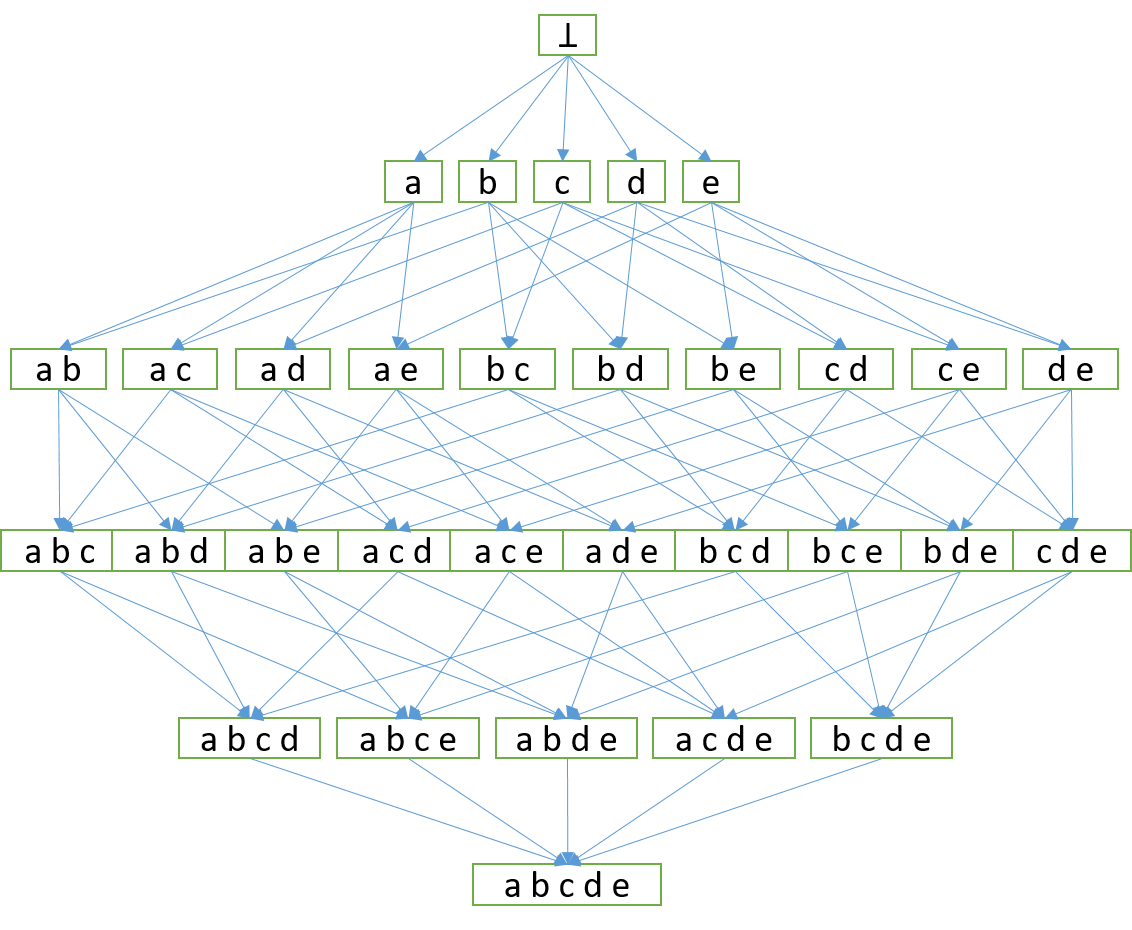
\includegraphics[width=5in]{chapters/lattices.png}
\caption{Lattice representing the search space of $\mathcal{D}$}
\label{lattice}
\end{figure}

\section{Big Data and Distributed Frameworks}
Today's shift towards horizontal scaling in hardware has highlighted the
need of distributed algorithms. Being able to analyze big data is a huge value from both an economic and social point of view. Unfortunately, traditional tools have demonstrated to be not reliable for dealing with such large amount of data.
%Starting from data storage, new solutions have to be developed to replace traditional relational database managements systems. 
% Thus, we
%are witnessing the explosion of distributed and parallel approaches, often
%accompanied with cloud-based services (e.g. Platform-as-a-Service
%tools)~\cite{ISPA13}.

Starting from data storage, new solutions had to be developed to replace traditional relational database managements systems. We have firstly witnessed the development of distributed file systems such as Google File System \cite{ghemawat2003google} and its derivative Hadoop Distributed File System~\cite{HDFS}. For the computational issues, already well-known parallel frameworks have shown their limitations due to fault tolerance and resiliency lacks. In the meanwhile, new processing models spread out. 
MapReduce~\cite{ArticoloMapReduceGoogle} is the most popular example of a generic batch-oriented distributed paradigm. With its reliable and fault-tolerant architecture, it allows to exploit the resources of more commodity machines (nodes). The ratio behind the spread of the paradigm is that 'shifts the computation to the data'.
In fact, taking advantage of the data locality, allowing the nodes to process just the shard of the data they store.

A MapReduce application consists of two main phases. In the first phase, called "map", each shard of the dataset is processed locally by each node of the commodity clusters, which output one or more key-values couples. Map results are exchanged among the cluster nodes and aggregate the tuples per key: this is the "shuffle" phase. This operation, which is very optimized, is one of the killer feature which a MapReduce-like algorithm should strongly exploit (it is also the unique communication among the nodes of the commodity cluster). Finally, the reduce phase is run for each unique keys and iterates through all the associated values.

Designed to cope with very large datasets, the Java-based framework Hadoop~\cite{HDFS} is the most widely adopted MapReduce implementation. It allows programmers not to concern to low level details and to focus just on the algorithm design.

However, Hadoop and MapReduce paradigm does not fit at all iterative processes. In this case, each iteration would require a complete read and transmission (shuffle phase) of the input dataset, which is critical when dealing with huge datasets. This issue motivated the development of a new in-memory distributed platform called Apache Spark~\cite{Zaharia_spark}. This framework, when possible, allows machines to cache data and intermediate results in memory, instead of reloading it from the disk at each iteration. Spark has also introduced a new type of data collection called RDD (Resilient Distributed Dataset). Every RDD modification is done just by the generation of another RDD, keeping trace of all the transformations in order to be able to regenerate data in case of failures. Furthermore, RDDs avoid on-disk materialization until not strictly mandatory, i.e. when an action requires a result to be returned to the driver program, saving resources in terms of communication and I/O costs. Spark supports both Graph-based and Streaming processes, demonstrating to be more flexible than Hadoop, still keeping full compatibility with the latter. 

Because of the winning features of Hadoop and Spark, testified by their spread in the academic environment, in this dissertation we will focus into these distributed frameworks, analyzing the best-in-class Hadoop and Spark-based works and utilizing their paradigm for further advancements of the state of the art.

However, Hadoop and Spark are
not the only frameworks supporting the parallelization of Data mining
algorithms. GraphLab~\cite{graphlab}, Google Pregel~\cite{pregel} and its
open-source counterpart Giraph~\cite{giraph} are fault-tolerant, graph-based
framework while SimSQL~\cite{simsql}, for instance, exploits an SQL-based
approach. Distributed systems are popular also because they became very easy to
use: as already stated, Message Passing Interface (MPI)~\cite{mpi}, one of the most adopted
framework in academic environment, works efficiently only on very low level
programming such as C.

\subsection{Hadoop and Spark Machine Learning Libraries}
In recent years the
success of these distributed platforms was supported by the introduction of open
source libraries of machine learning algorithms.
%These are very precious for the academic world
%since they allow researchers to save time for implementation or to use the
%algorithms as reference baseline for further optimizations.
% We strongly consider
%the presence of these libraries as a real advantage of a framework.
Mahout~\cite{Mahout} for Hadoop has represented one of the most popular
collection of Machine Learning algorithms, containing implementations in the
areas such as clustering, classification, recommendation systems, etc. All the
current implementations are based on Hadoop MapReduce.
MADlib~\cite{madlib},
instead, provides a SQL toolkit of algorithms that run over Hadoop. Finally,
MLLib~\cite{MLLib} is the Machine Learning library developed on Spark, and it is
rapidly growing up. MLLib allows researchers to exploit Spark special features
to implement all those applications that can benefit from them, e.g. fast
iterative procedures.

\section{Big Data and FIM (maybe should put this before 2.2)}
In this Section we will motivate the need of scalable frequent itemeset mining algorithms and their relations with input dataset size and
minimum support threshold. After that, the issues related to the problem statement will be discussed.

\textbf{Input size and minimum support value.} As already largely discussed, we are witnessing an explosive increasing of data availability. Process and support this extremely large amount of data is very challenging. Data mining algorithms, for their nature, as better detailed in the last part of this Section, are among the hardest processes to parallelize. Specifically, the parameters which most affect the mining are 2. The first, as predictable, is the input data size, while the second is the minimum support threshold. 

The first issue is already intuitive since a bigger data collection is harder to analyze. The problem is caused by the inner data structure (e.g., FP-tree \cite{Han00}, Enumeration Tree \cite{Zaki_Carpenter}, Prefix Tree \cite{Zaki97newalgorithms}, ...) leveraged by the algorithm itself to explore the search space. Larger datasets lead to larger data structures built by the algorithm itself. Larger data structures require large amount of memory and computational resources to be maintained and explored.

The second issue is related to minimum support threshold, which, in our problem, is directly mirrored to the targeted depth of the analysis. 
Even for datasets not belonging to big data environment, a very low support 
extraction could require huge amount of resources. 
The lower it is, the more challenging in terms of resource the mining will be. 
Therefore, it is likely to occur that frequent itemset miner is easily able to complete the itemsets extraction with a certain minimum support threshold, and running out of memory with the same input and a lower support. 
Even in this case, the motivations are related to the inner structure used by the algorithms to explore the search space~\cite{goethals2003survey}. A low minimum support threshold leads to a deeper exploration of the search space. For some algorithms like Apriori~\cite{Agr94}, it could lead to the generation and testing of all the possible combinations of the dataset items. The mining considers any possible items co-occurrency and it can happen that the output of the process exceeds the input data size (as clearly shown in Tables \ref{back_horizontalexampledataset} and \ref{back_frequent}). In addition, please note that the size and the complexity of these structure do not scale linear with the minimum support threshold \cite{KumarBook},~\cite{goethals2003survey}. For these reasons, this parameter is very important analyzing the performance of a frequent itemset mining algorithm. 







%
%
%
%
%
%
%
%\begin{table}[]
%
%\centering
%
%\caption{Example of frequent itemset mining with minsup of 50\% \label{toy_mining}}
%
%\begin{tabular}[t]{|c|c|}
%\hline
%\multicolumn{2}{|c|}{$\mathcal{D}$}\\
%\hline
%\hline
%tid & items \\
%\hline
%1 &	A B C D \\
%\hline
%2 &	A C D E\\
%\hline
%	3 &B C D E\\
%\hline
%4 &	A D E \\
%\hline
%
%\end{tabular}\qquad
%
%\begin{tabular}[t]{|c|l|}
%\hline
%\multicolumn{2}{|c|}{$TT$}\\
%\hline
%\hline
%	item & tidlist \\ \hline
%	A & 1,2,3,4,5 \\ \hline
%	B & 1,5 \\ \hline
%	C & 1,3 \\ \hline
%	D & 2,5 \\ \hline
%	E & 2,3 \\ \hline
%\end{tabular}\qquad
%\begin{tabular}[t]{|c|c|}
%\hline
%\multicolumn{2}{|c|}{Frequent Itemsets}\\
%\hline
%\hline
%itemsets & Support \\
%\hline
%A & 3\\
%\hline
%B & 2 \\
%\hline
%C & 3\\
%\hline
%D & 4\\
%\hline
%E& 3 \\ 
%\hline
%	A C & 2\\
%\hline
%	A D & 3\\
%\hline
%	A E & 2\\
%\hline
%	B C & 2\\
%\hline
%B D & 2\\
%\hline
%	C D & 3\\
%\hline
%	C E & 2\\
%\hline
%	D E & 3\\
%\hline
%A C D & 2\\
%\hline
%A D E& 2\\
%\hline
%B C D & 2\\
%\hline
%C D E & 2\\
%\hline
%\end{tabular}\qquad
%
%\end{table}
%




These two aspects are the most critical issues for itemset extraction. As we will see in Chapters \ref{survey} and \ref{pampa}, also input data distribution has an impact. For the sake of clarity, for the moment, we ignore this feature, which is very dependent on the algorithms nature. 
 

\textbf{Motivations.} Now, let us focus on the reasons behind the needs to mine huge datasets and/or extract itemsets with low minimum support thresholds. Focusing on the first aspect, the need of scalability in terms of input dataset size is an obvious consequence of the requirement to analyze huge data collections. Indeed, in big data analysis domain, frequent itemset mining is very useful tool. For instance, thinking about the summarization properties of frequent itemsets, we can assume that the larger is the dataset, the more essential would be its summarization.

%Now, let us focus on the need of lowering the minimum support threshold. 
As already mentioned, even low supports could represent very challenging mining processes. 
The reader could wonder about the need of such amount of frequent itemsets, given that, one of the most intuitive usage examples are related to data summarization.
However, in many applications, frequent pattern mining can be considered as a preprocessing than a final step. One of the most intuitive contexts is the "infrequent" itemset extraction and outlier detection algorithms \cite{cagliero2014infrequent},\cite{brauckhoff2012anomaly}. 
The need of a deep extraction is also motivated by the hitches to include any interestingness measures (apart from the support) into the extraction process. Hence, a very common behavior is to extract as many itemsets as possible and then apply any sort of interestingness filter. 
For instance, already in this dissertation, will be introduced a work, in which a special type of itemsets is mined from a set of frequent itemsets (see Chapter \ref{nemico} for further details).


\textbf{Challenges.} The parallelization of the mentioned data structures represents the main contribution behind the development of distributed and parallel frequent itemset mining algorithms. Like almost all the data mining tools, this technique, as already discussed, does not fit parallel and/or distributed implementations. 
%The first issue is related to the nature of the problem which assume a full knowledge of the data. 
In distributed an parallel domains, an ideal approach assumes to divide the problem into independent non-overlapping sub-problems, which can be assigned to commodity cluster nodes. In this way, (i) the resource are completely exploited and (ii) the communication costs, a concrete bottleneck in distributed environment, are reduced as much as possible.

In FIM environment, the task that should be parallelized is the search space exploration, which is done through ad-hoc data structures. As detailed in Chapters \ref{survey} and \ref{pampa}, all the distributed FIM algorithms smartly split and distribute the processing of these data structures, most of the them in "divide and conquer" fashion. This technique overcomes the main memory issues.
However, this split is often sub-optimal:
\begin{itemize}
\item First, in order to be independent for the mining task related to the respective algorithm, the set of resulting partitions could overlap each other (please note that the overlapping degree is dependent from the data distribution). Overlapping partitions entails that the global memory of the cluster should be larger than the already huge input data, storing redundant data \cite{Mahout},\cite{pampa_v1} which can lead to redundant and useless output \cite{bigfim},\cite{pampa_v1}. Furthermore, it increases the communication costs because more data have to be transmitted across the network.

\item In addition, in centralized algorithms, some pruning techniques are often used to limit the search space exploration, saving time and resources. Some of the challenges related to the parallelization of exploration task parallelization are the difficulties related to these pruning techniques, which assumes a state centralized memory. In \cite{pampa_v1}, we have addressed this issue, introducing a trade-off among the benefits related to a centralized memory ("state") and the ones related to the degree of parallelization (i.e. number of independent parallel tasks) (further details in Chapter \ref{pampa}).
\end{itemize}

These are the main challenges and the possible drawbacks related 
to a parallel implementation of frequent itemset mining algorithms. 
In the next Chapter we will evaluate how the best-in-class state of the art algorithms have addressed these questions. In Chapter \ref{pampa}, instead, we will introduce our solution concerning parallel \textit{high-dimensional} frequent pattern mining. 



\chapter{Frequent Itemset Mining for Big Data: an experimental review}\label{survey}

\section{Introduction}
\label{Introduction}
%In recent years, the increasing capabilities of recent applications to produce
%and store huge amounts of information has changed dramatically the importance of
%the intelligent analysis of big data. The interest towards data mining, an
%important set of techniques useful to extract effective and usable knowledge
%from data, has risen.
%This trend is noticeable in both the academic and the industrial
%domains.
%For researchers, the big data analytics scenario is very challenging. Often,
%indeed, the application of traditional data mining techniques to such large
%volumes of data is not straightforward. It is not only a matter of computational
%power or memory; some of the most popular techniques had to be redesigned from
%scratches to fit the new environment.
%On the other side, companies are
%interested in the strategic benefits that big data could deliver, even directly.
%In~\cite{junque2013predictive}, the authors present a study to illustrate that
%larger data indeed can be more valuable assets for predictive analytics. The
%deduction is that institutions with larger collections of data and, of course,
%the skill to take advantage of them, can obtain a competitive advantage over
%institutions without. Data mining, together with machine learning~\cite{DBLP:journals/bdr/Al-JarrahYMKT15}, is the main tool on which big data analytics
%rely on and it includes different types of techniques: (i) clustering
%algorithms to discover hidden structures in unlabelled
%data~\cite{Xu_2005SurveyClustering}, (ii) frequent itemsets mining and association
%rules analysis to discover interesting correlations and
%dependencies~\cite{Han_2007SurveyFIM}, and finally, (iii) supervised learning
%techniques to extract a function or a model that best approximates the
%distribution of the input dataset to map or label new data
%examples~\cite{AggarwalBookClassification}.
Existing data mining algorithm revealed to be very efficient on typical datasets but
very resource intensive when the size of the input dataset grows up. In general,
applying data mining techniques to big data collections has often entailed to
cope with computational costs that represent a critical bottleneck. Furthermore,
the shift towards horizontal scaling in hardware has highlighted the need of
distribution/parallelization of data analytics techniques. 

Effective and efficient analytics algorithms have been proposed during the last
years to better utilize the available hardware resources and distributed
computing frameworks. Here we focus on itemset mining algorithms because thery
represent exploratory approaches widely used to discover frequently co-occurring
items from the data. These algorithms have been widely exploited in different
application domains (e.g., network traffic data~\cite{ApilettiBCCG13},
healthcare~\cite{META-TIST-2015}, biological data~\cite{DBLP:conf/sigmod/CongXPTY04}, energy
data~\cite{NostroENDM2016_senzacrossref}, images~\cite{zaianeimage},  open
linked data~\cite{BCOpenLinkedData}, document and data summarization~\cite{BaralisCFG15},~\cite{DBLP:journals/cg/LopesPPM07},~\cite{Mampaey:2011:TMI:2020408.2020499},
to support different targeted analyses.

Although different algorithms have been proposed to perform the computationally
intensive frequent itemset mining task, also in the distributed frameworks, no
algorithm is universally superior. Several aspects influence which algorithm
performs best, including input data cardinality and data distribution, adopted
strategies to process the data into independent tasks, strategies to reduce the
communication costs. The algorithm selection for a given analytics case study is
usually manually performed based on analyst expertise and it is very time
consuming. To help the analyst in the algorithm selection process, the work introduced in this chapter presents 
an experimental comparison of different scalable itemset mining
algorithms. Specifically, as summarized in Table \ref{survey_recap}, the
contribution of this review includes:
\begin{itemize}
\item The discussion of the state-of-the-art itemset mining algorithms dealing
with huge data collections to analyze how technological development efficiently
support the continuous design of more scalable and more efficient algorithms. We
selected the most two widespread and recent distributed frameworks as
Hadoop~\cite{HDFS}, Apache Spark~\cite{Zaharia_spark} to set the experimental
scenario. We selected the five algorithms, to
perform the itemset mining discovery on distributed environment. 	These
algorithms (i.e., Mahout PFP~\cite{Mahout}, Mllib PFP~\cite{MLLib},
BigFIM~\cite{bigfim}, DistEclat~\cite{bigfim}, YAFIM~\cite{YAFIM}) cover the
different search space strategies adopted in the centralized architecure to
efficiently address the mining activity by effectively dealing with different
data distribution.
\item
The definition of four evaluation criteria to characterize both  the algorithmic
strategies and the distributed implementation as well.
\item
A detailed comparative analysis of the selected, running on either Spark or
Hadoop framework, with a thoroughly discussion on interesting results got by
performing a large set of experiments on real and synthetic datasets.
Specifically, we run more than 250 experiments on 14 synthetic datasets and 2 real datasets to
evaluate the algorithm performance, load balancing and communication cost as
well.
\item
The discussion of the lessons learned to share general advices gained from the
experience of performing the in-depth comparative analysis.
\item
The discussion of some open issues that should be addressed to support a more
effective and efficient data mining process on very large datasets.
\end{itemize}

The results described in this Chapter have been published as \textbf{aggiungere citazioni minisurvey big dap e, una volta pubblicato, speriamo, survey altro.} and are organized as follow. Section~\ref{criteria} presents the
evaluation criteria considered in this study. Section~\ref{algorithms} discusses
the selected algorithms, while in
Section~\ref{experimental} we benchmark the algorithms with a large set of
experiments on both real and synthetic datasets.
Section~\ref{lesson} summarizes the lessons learned from our evaluation
analysis, while Section~\ref{openissues} discusses some research directions to
be addressed to support a more effective and efficient data mining process on
big data collections. Section~\ref{conclusion} provides a brief summary of this
review.


%
%\section{Apache Hadoop and Spark}
%\label{bigdata}
%

Today's shift towards horizontal scaling in hardware has highlighted the
need of distributed algorithms. Thus, we
are witnessing the explosion of distributed and parallel approaches, often
accompanied with cloud-based services (e.g. Platform-as-a-Service
tools)~\cite{ApilettiBCCG13}.
MapReduce~\cite{ArticoloMapReduceGoogle} can be considered the most popular
approach of the past decade. Designed to cope with very large datasets,
Hadoop~\cite{HDFS} is the most widely adopted MapReduce implementation.
In the last couple of years, instead, Apache Spark~\cite{Zaharia_spark}
has become the favourite platform for large scale data analytics,
outperforming Hadoop
performance thanks to its distributed memory abstraction. Hadoop and Spark are
not the only frameworks supporting the parallelization of Data mining
algorithms. GraphLab~\cite{graphlab}, Google Pregel~\cite{pregel} and its
open-source counterpart Giraph~\cite{giraph} are fault-tolerant, graph-based
framework while SimSQL~\cite{simsql}, for instance, exploits an SQL-based
approach. Distributed systems are popular also because they became very easy to
use: Message Passing Interface (MPI)~\cite{mpi}, one of the most adopted
framework in academic environment, works efficiently only on very low level
programming such as C.


In this review we analyse and evaluate the most effective approaches developed
on top of the Apache Hadoop~\cite{HDFS} and Spark~\cite{Zaharia_spark}
frameworks.
Thanks to their architecture which allows programmers to focus only on the
algorithmic issues,
leveraging the high level programming environment, these frameworks represent
the current de-facto standard in the Big Data environment.
Both of them support the MapReduce paradigm,
a distributed programming model introduced by
Google~\cite{ArticoloMapReduceGoogle}
to support its data intensive processing.
A MapReduce application consists of two main phases,
whose names are map and reduce. The map
function is fed with a shard of the input dataset on each node;
after the processing it outputs one or more key-value couples.
Map results are exchanged among the cluster nodes:
this is the optional shuffle phase.
Finally, the reduce phase is run for each unique key and iterates
through the values that are associated with that key.

%The main benefit of the paradigm is the optimized shuffle operation
% that should be exploited to achieve the best performance.
% Not all algorithms can be straightforward adapted to the MapReduce paradigm.
% In~\cite{chu2007map}, the authors designed Statistical Query model
% as a judging condition for an efficient and balanced implementation.

Hadoop has become very popular in the last decades; it allows programmers not to
concern about inter-process communication and low-level details but to focus on
the problem to be solved. The success of Hadoop and MapReduce is due to the
paradigm
that shifts the computation to the data: thanks to the Hadoop Distributed File
System (HDFS), it takes advantages of data locality allowing the nodes to
process the data they store.
The MapReduce paradigm is designed for batch processing:
iterative processes do not fit efficiently since, often,
each iteration requires a new reading phase from the disk.
This feature is critical when dealing with huge datasets.
This issue motivated the improvements introduced by Spark.
Apache Spark is a general purpose in-memory
distributed platform. It enables machines to cache data and intermediate results
in memory, instead of reloading them from the disk at each iteration, through
the introduction of Resilient Distributed Datasets (RDD). A RDD is a read-only,
partitioned collection of records obtained from another RDD or from HDFS.
RDDs can avoid on-disk materialization since their creation process,
as a series of transformations (the lineage), is preserved,
so that they can be recreated when needed, even if this is an expensive process.
%Recreating from scratch RDDs can be resource intensive, so algorithms
%characterised by asynchronous fine-grained processes can be slowed down.
%However, Spark offers more use applications,
Spark supports both graph and streaming processes, overcoming the
limitations of the MapReduce batch-oriented paradigm, although maintaining a
full
compatibility with the latter.
Adding flexibility beyond the two-stage model of
MapReduce, Spark can provide complex Direct Acyclic Graph (DAG) data
flows. Spark also supports different development languages, such as
Java, Python and Scala, while Hadoop supports only Java.

\subsection{Hadoop and Spark Machine Learning Libraries}
In recent years the
success of these distributed platforms was supported by the introduction of open
source libraries of machine learning algorithms.
%These are very precious for the academic world
%since they allow researchers to save time for implementation or to use the
%algorithms as reference baseline for further optimizations.
% We strongly consider
%the presence of these libraries as a real advantage of a framework.
Mahout~\cite{Mahout} for Hadoop has represented one of the most popular
collection of Machine Learning algorithms, containing implementations in the
areas such as clustering, classification, recommendation systems, etc. All the
current implementations are based on Hadoop MapReduce.
MADlib~\cite{madlib},
instead, provides a SQL toolkit of algorithms that run over Hadoop. Finally,
MLLib~\cite{MLLib} is the Machine Learning library developed on Spark, and it is
rapidly growing up. MLLib allows researchers to exploit Spark special features
to implement all those applications that can benefit from them, e.g. fast
iterative procedures.


%\section{Frequent itemset mining}
%\label{Preliminaries}
%
\begin{figure}[!t]
%\renewcommand{\arraystretch}{1.3}
%\centerline

{\subfloat[Horizontal representation of $\mathcal{D}$]{
\label{horizontalexampledataset}
\begin{tabular}{|c|l|}

\hline
\multicolumn{2}{|c|}{$\mathcal{D}$}\\
\hline
\hline
	tid & items \\
\hline
	1 & a,b,c,l,o,s,v \\
\hline
	2 & a,d,e,h,l,p,r,v \\
\hline
	3 & a,c,e,h,o,q,t,v \\
\hline
	4 & a,e,f,h,p,r,v \\
\hline
	5 & a,b,d,f,g,l,q,s,t \\
\hline
\end{tabular}}}%
\hfil
{\subfloat[Vertical representation of $\mathcal{D}$]{
\label{TTexampledataset}
\begin{tabular}{|l|l|}
\hline
\multicolumn{2}{|c|}{Vertical Representation}\\
\hline
\hline
	item & tidlist \\ \hline
	a & 1,2,3,4,5 \\ \hline
	b & 1,5 \\ \hline
	c & 1,3 \\ \hline
	d & 2,5 \\ \hline
	e & 2,3,4 \\ \hline
	f & 4,5 \\ \hline
	g & 5 \\ \hline
	h & 2,3,4 \\ \hline
	l & 1,2,5 \\ \hline
	o & 1,3 \\ \hline
	p & 2,4 \\ \hline
	q & 3,5 \\ \hline
	r & 2,4 \\ \hline
	s & 1,5 \\ \hline
	t & 3.5 \\ \hline
	v & 1,2,3,4 \\ \hline
\end{tabular}}}%

\caption{Running example dataset $\mathcal{D}$}
\label{exampledataset}
\end{figure}
In this section, a basic introduction to frequent itemset mining will
be given to the readers.
Let $\mathcal{I}$ be a set of items. A transactional dataset $\mathcal{D}$
consists of a set of transactions $\{t_1, \dots, t_n\}$.
Each transaction $t_i\in \mathcal{D}$ is a collection of items
(i.e., $t_i\subseteq \mathcal{I}$)
and it is identified by a transaction identifier ($tid_i$).
Figure~\ref{horizontalexampledataset} reports an example of a transactional
dataset with 5 transactions.

% %The dataset reported in Figure~\ref{horizontalexampledataset} is used as a
% running example through the paper.
% %
% %An itemset $I$ is defined as a set of items (i.e., $I\subseteq\mathcal{I}$) and
% it is characterized by a tidlist and a support value.
% %The tidlist of an itemset $I$, denoted by $tidlist(I)$, is defined as the set
% of tids of the transactions in $\mathcal{D}$ containing $I$,
% %while the support of $I$ in $\mathcal{D}$, denoted by $sup(I)$, is defined as
% the ratio between the number of transactions in $\mathcal{D}$ containing $I$
% %and the total number of transactions in $\mathcal{D}$ (i.e.,
% $|tidlist(I)|/|\mathcal{D}|$).
% %For instance, the support of the itemset \textit{\{aco\}} in
% %the running example dataset $\mathcal{D}$ is 2/5 and its tidlist is $\{1,3\}$.
% %An itemset $I$ is considered frequent if its support is greater than a
% user-provided minimum support threshold $minsup$.

An itemset $I$ is defined as a set of items (i.e., $I\subseteq\mathcal{I}$)
and it is characterized by a support value, which is denoted by $sup(I)$ and
defined as the ratio between the number of transactions in $\mathcal{D}$
containing $I$ and the total number of transactions in $\mathcal{D}$.
%(i.e., $|tidlist(I)|/|\mathcal{D}|$).
In the example dataset in Figure~\ref{horizontalexampledataset}, for instance,
the support of the itemset \textit{\{aco\}} is 2/5. . This value represents the frequency of occurrence of the itemset in the dataset.

Given a transactional dataset $\mathcal{D}$ and a minimum support
threshold $minsup$, the Frequent Itemset Mining \cite{KumarBook} problem
consists in extracting the complete set of frequent itemsets
from $\mathcal{D}$.



Many subsets of frequent itemsets exist.
In this paper, we focus on closed itemsets.
Closed itemsets~\cite{ClosedPasquier1999} are a
particular and valuable subset of frequent itemsets, being
a concise but complete representation of frequent itemsets. 
Precisely, an itemset $I$ is closed if none of its supersets (i.e. the set of itemsets which include $I$) has the same support count as $I$.

%If an itemset is frequent, all of its subsets are frequent for the \textit{monotonic property}.
%For the same rule, if an items or an itemset is not frequent, none of its supersets are frequent. In addition, an items
% or itemset $I$ is closed in  $\mathcal{D}$ if there exists no superset that has the same support count as  $I$.\\

A transactional dataset can also be represented in a vertical format, which is
usually a more effective representation for datasets characterised by an average
number of items per transaction orders of magnitudes larger than the number of
transactions.
In this representation, each
row consists of an item $i$ and the list of transactions in which it appears,
also called $tidlist(\{i\})$.
For instance, the tidlist of the itemset \textit{\{aco\}} in
the example dataset $\mathcal{D}$ is $\{1,3\}$.
Figure~\ref{TTexampledataset} reports the transposed representation of the
running example reported in Figure~\ref{horizontalexampledataset}. The main
advantage of the vertical format is the possibility to obtain the tidlist of
an itemset just intersecting the tidlists of the included items, without the
need of a full scan of the dataset.




%\section{Evaluation criteria}
%\label{criteria}
%The main target of this review is to build a structured comparison among the
most popular frequent itemset miners in distributed environments.
For this reason, we define a set of criteria
which can be divided into two groups, summarized in Table~\ref{tab:evalcriteria}.

The first group, named \textit{algorithmic strategy}, is strictly related to the centralized frequent itemset algorithms from which the distributed implementations are derived. 
Itemset discovery algorithms, proposed for the distributed frameworks, are not designed from scratches to be distributed or parallelized. Often, the main contribution introduced in the domain is the implementation of well-known techniques to distributed environment. Thus, the main research efforts are moved from the algorithm design to the following points:

\begin{itemize}

\item The distribution
of tools or algorithms that were not designed to be distributed (i.e. splitting
the computation load into more than one node). In addition, data mining
algorithms are often characterized by the need of a full knowledge of the
problem or data. In other words, data mining problems are often not
"embarassingly parallelizable". This issue makes the distribution very
challenging.

\item A well-engineered transposition to distributed frameworks,
exploiting the advantages and features of the platforms. For instance,
exploiting data locality in MapReduce-based implementations provides a
fundamental performance boost. Another example is the optimized ``shuffle \&
sort'' phase, which represents the unique phase in which data can be sent to other
nodes. Transposing an algorithm into MapReduce can be very challenging because
of its limitations, whereas one of the advantages of Apache Spark over Hadoop
is a  greater flexibility.

\end{itemize}

Hence, the underlying centralized algorithms
are very important to describe and evaluate the scalable approaches. Some of
their features are directly inherited by the distributed algorithms.

Specifically, we have selected two criteria, as reported in Table~\ref{tab:evalcriteria}, directly inherited from the underlying centralized approaches, named the candidate itemset generation phase~\cite{goethals2003survey}. 

\begin{enumerate}

\item \textit{The search space exploration strategy} allows decomposing the mining task into a set of smaller tasks to dramatically reduce the computation cost. Different strategies have been exploited in performing the itemset mining as divide-and-conquer, depth-first methods or level-wise, breadth-first generation methods.  Each strategy can yield good performance when dealing with a given data distribution. 

\item \textit{The data distribution}. Each collection of data is characterized by a given distribution varying based on the number of transactions, average transaction length (average number of objects in a given transaction, and the cardinality of different objects. Datasets are
usually characterized by an inherent sparseness when a large number of transactions appear with a limited/shorter average transaction length, and a large variety of different objects/items. The sparseness in data distribution
increases with data volume and cardinality of different objects.
Although a formal and universal definition of data distribution is not yet available in the domain of itemset mining, it is well-known that a given algorithm is typically suited for a given data distribution, thus its performance are the best for some datasets or under some input parameter values and the worst in other cases. In general, the execution cost of a given algorithm tends to increase when dealing with dense datasets or large data volume with an inherent sparseness but with low support thresholds. In these both conditions, a large number of itemsets have to be generated. \end{enumerate}

The performance of the algorithms that adopt a level-wise or breadth-first exploration  (i.e. algorithms that generate candidate itemsets of length $k$ from itemsets of length $k-1$) is negatively affected by a large average transaction width, because more candidate itemsets must be examined~\cite{KumarBook}. Since average transaction width is strongly related to the input data distribution, there exists a relationship between the exploration strategy and the input dataset distribution. For example, Apriori-based algorithms~\cite{Agr94}, detailed in Subsection~\ref{bigfim}, with their breadth-first exploration approach, better fit datasets characterized by
sparse distributions, i.e. low correlation among patterns and high item cardinality.



The second set of evaluation criteria is related to the distributed nature of
the processing. They are often undervalued in the data mining context but
represent critical
issues~\cite{afrati2012designing},~\cite{leskovec2014mining}.

\begin{enumerate}

\item Communication costs: this issue is often underestimated in distributed
algorithms, but they represent the most likely bottleneck of a distributed
system~\cite{sarma2013upper}. In the design phase, most of the researchers focus
only on the computational costs and the need to split them among the nodes. The
result is that a great amount of data is sent through the network, making
communication costs much higher than computational costs.
% In addition, as already
% mentioned, many data minings algorithms were designed for centralized systems,
% ignoring these kinds of factors. However, the data locality paradigm is one of
% the reason of the effectiveness of distributed platforms such as Hadoop or
% Spark. Thus, the implementations in this review will be evaluated also through
% the care or attention devoted to this aspect.

\item Load balancing: since one of the main goals of a distributed
approach is to decrease the overall execution time, load balancing is required
to efficiently reach such objective. An unbalanced load
undermines the advantages of a parallel environment: the overall execution time
is that of the slowest, most loaded node. In a fully unbalanced environment, the
worst case scenario leads to no benefits from parallelization while still
incurring all the overheads of coordinating a rather complex distributed system.

\end{enumerate}

A review of the evaluation criteria is presented in
Table~\ref{tab:example1}. After a qualitative review of the algorithms in
Section~\ref{algorithms}, in Section~\ref{experimental} an experimental
performance evaluation is provided.

%
%\begin{table*}[]
%\scriptsize
%\centering
%\caption{Overview of valution criteria. \label{tab:evalcriteria}}
%\begin{tabular}{| c|c|c|c|}
%\hline {\bf Class Name} & {\bf Property of} & {\bf Criterion name} & {\bf Domain} \\ \hline
%\hline Algorithmic & Centralized  & The search space & $\{$Depth First,  \\
%strategy & approaches & exploration strategy & Breadth First $\}$  \\
%\hline 
%& & Data distribution & $\{$dense, sparse$\}$ \\  \hline
%
%\hline 
%Distributed & Distributed  & Communication & $\{$Yes, No$\}$ \\
%processing & approaches & cost handling & \\
%\hline 
%& & Load balancing & $\{$Yes, No$\}$ \\
%& & handling &  \\
%\hline 
%\end{tabular}
%\end{table*}


\begin{table*}[]
\scriptsize
\centering
\caption{Overview of evaluation criteria. \label{tab:evalcriteria}}
\begin{tabular}{| c|c|c|c|}
\hline \textbf{Class Name}                                                               & \textbf{Property of}                                                              & \textbf{Criterion name}                                                                           & \textbf{Domain}                                                                             \\ \hline \hline
\multirow{3}{*}{\begin{tabular}[c]{@{}c@{}}Algorithmic \\ strategy\end{tabular}}  & \multirow{3}{*}{\begin{tabular}[c]{@{}c@{}}Centralized\\ approaches\end{tabular}} & \multirow{2}{*}{\begin{tabular}[c]{@{}c@{}}The search space \\ exploration strategy\end{tabular}} & \multirow{2}{*}{\begin{tabular}[c]{@{}c@{}}\{ Depth First,\\  Breadth First\}\end{tabular}} \\
                                                                                  &                                                                                   &                                                                                                   &                                                                                             \\ \cline{3-4} 
                                                                                  &                                                                                   & Data distribution                                                                                 & \{ dense, sparse \}                                                                         \\ \hline
\multirow{4}{*}{\begin{tabular}[c]{@{}c@{}}Distributed\\ processing\end{tabular}} & \multirow{4}{*}{\begin{tabular}[c]{@{}c@{}}Distributed\\ approaches\end{tabular}} & \multirow{2}{*}{\begin{tabular}[c]{@{}c@{}}Communication\\ cost handling\end{tabular}}            & \multirow{2}{*}{\{ Yes, No \}}                                                               \\
                                                                                  &                                                                                   &                                                                                                   &                                                                                             \\ \cline{3-4} 
                                                                                  &                                                                                   & \multirow{2}{*}{\begin{tabular}[c]{@{}c@{}}Load balancing\\ handling\end{tabular}}                & \multirow{2}{*}{\{ Yes, No \}}                                                               \\
                                                                                  &                                                                                   &                                                                                                   &                                                                                             \\ \hline
\end{tabular}
\end{table*}

\label{Preliminaries}
\begin{figure}[!t]
{\subfloat[Horizontal representation of $\mathcal{D}$]{
\label{back_horizontalexampledataset}
\begin{tabular}{|c|l|}
\hline
\multicolumn{2}{|c|}{$\mathcal{D}$}\\
\hline
\hline
	tid & items \\
\hline
	1 &	a b c d \\
\hline
2 &	a c d e\\
\hline
	3 &b c d e\\
\hline
4 &	a d e \\
\hline
\end{tabular}}}
\hfil
{\subfloat[Transposed representation of $\mathcal{D}$]{
\label{back_TTexampledataset}
\begin{tabular}{|c|l|}

\hline
\multicolumn{2}{|c|}{$TT$}\\
\hline
\hline
	item & tidlist \\ \hline
	a & 1,2,4 \\ \hline
	b & 1,3 \\ \hline
	c & 1,2,3 \\ \hline
	d & 1,2,3,4 \\ \hline
	e & 2,3,4 \\ \hline
\end{tabular}}}%
\hfil
{\subfloat[Frequent itemset extracted from $\mathcal{D}$ with a minsup=2 ]{
\label{back_frequent}
\begin{tabular}{|c|l|}
\hline
\multicolumn{2}{|c|}{Frequent itemsets}\\
\hline
\hline
itemset & support \\
\hline
a & 3\\
\hline
b & 2 \\
\hline
c & 3\\
\hline
d & 4\\
\hline
e& 3 \\ 
\hline
	a c & 2\\
\hline
	a d & 3\\
\hline
	a e & 2\\
\hline
	b c & 2\\
\hline
b d & 2\\
\hline
	c d & 3\\
\hline
	c e & 2\\
\hline
	d e & 3\\
\hline
a c d & 2\\
\hline
a d e& 2\\
\hline
b c d & 2\\
\hline
c d e & 2\\
\hline
\end{tabular}}}%
\caption{Running example dataset $\mathcal{D}$}
\label{back_exampledataset}
\end{figure}

A frequent itemset represents frequently  co-occurring items in a transactional dataset. 
More formally, let $\mathcal{I}$ be a set of items. A transactional dataset $\mathcal{D}$
consists of a set of transactions $\{t_1, \dots, t_n\}$.
Each transaction $t_i\in \mathcal{D}$ is a collection of items
(i.e., $t_i\subseteq \mathcal{I}$)
and is identified by a transaction identifier ($tid_i$).
Figure~\ref{back_horizontalexampledataset} reports an example of a transactional
dataset with 4 transactions.


An itemset $I$ is defined as a set of items (i.e., $I\subseteq\mathcal{I}$)
and is characterized by a support value, which is denoted by $sup(I)$ and
defined as the ratio between the number of transactions in $\mathcal{D}$
containing $I$ and the total number of transactions in $\mathcal{D}$.
In the example dataset in Figure~\ref{back_horizontalexampledataset}, for example,
the support of the itemset \textit{\{a,c,d\}} is 50\% (2/4). This value represents the frequency of occurrence of the itemset in the dataset. An itemset $I$ is considered frequent if its support is greater than a
user-provided minimum support threshold $minsup$. Figure~\ref{back_frequent}
reports the frequent itemset extracted from $\mathcal{D}$ with a minsup value equal to 50\% (i.e., an absolute support equal to 2).

Given a transactional dataset $\mathcal{D}$ and a minimum support
threshold $minsup$, the Frequent Itemset Mining \cite{SurveyHan2007} problem
consists in extracting the complete set of frequent itemsets
from $\mathcal{D}$.

The dimension of the search space can be represented as a lattice, whose top is an empty set. Its size increases exponentially with the number of items~\cite{goethals2003survey}.
In Figure~\ref{lattice}, the lattice related to our running example is shown.

\begin{figure}[!t]
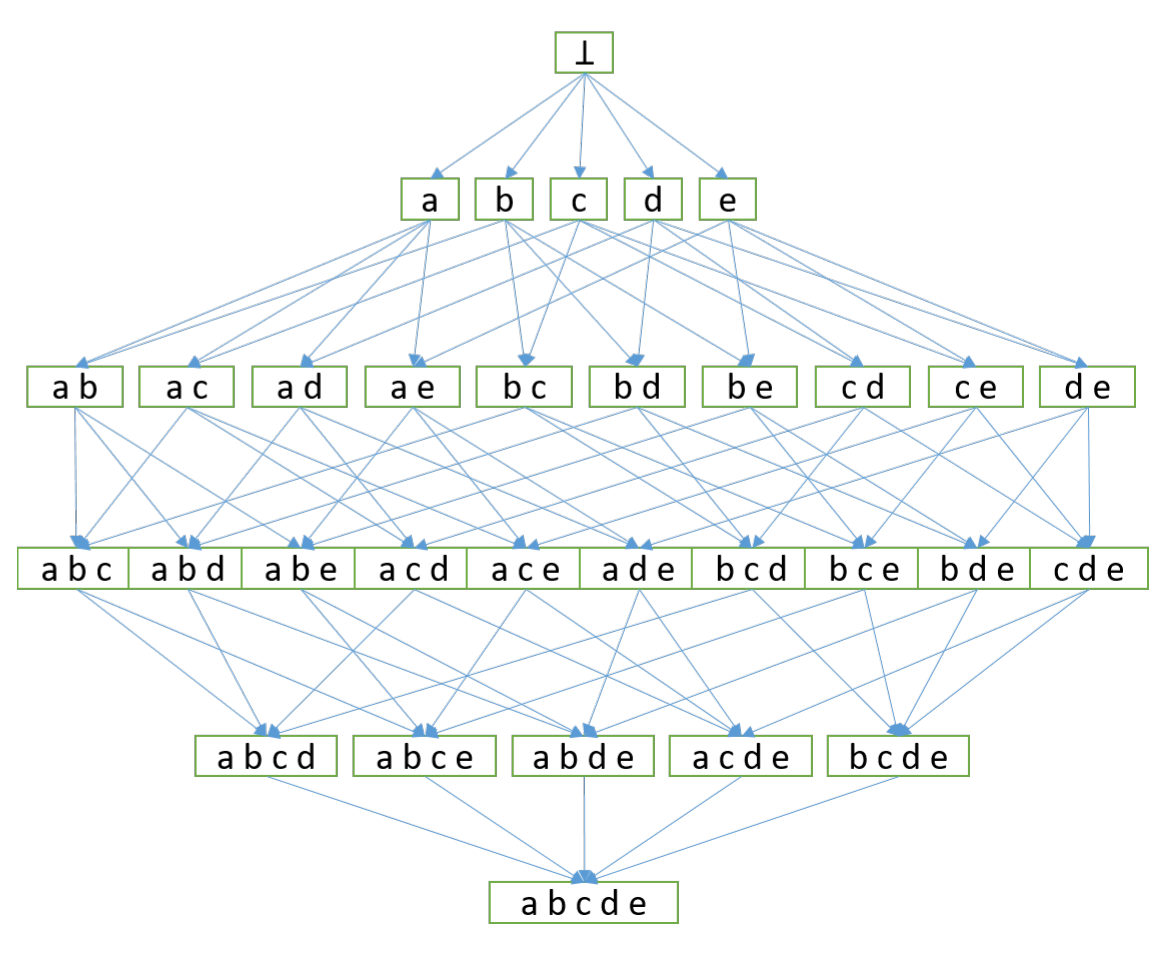
\includegraphics[width=5in]{immagini/lattices.eps}
\caption{Lattice representing the search space based on the items appearing in the example dataset $\mathcal{D}$}
\label{lattice}
\end{figure}


In this paper, we focus on closed itemsets.
Closed itemsets~\cite{ClosedPasquier1999} are a
particular and valuable subset of frequent itemsets, being
a concise but complete representation of the set of frequent itemsets. 
Precisely, an itemset $I$ is closed if none of its supersets (i.e. the set of itemsets which include $I$) has the same support count as $I$. For instance, in our running example, given a $minsup=2$, the itemset \textit{\{a,d\}} is a closed frequent itemset (support=3). The itemset \textit{\{a,c\}}, instead, is a frequent itemset (support=2), but it is not closed because of the presence of the itemset \textit{\{a,c,d\}} (support=2). 

A transactional dataset can also be represented in a vertical format, in which each
row represents an item $i$ and the list of tids of the transactions in which it appears,
also called $tidlist(\{i\})$.
For instance, the tidlist of the item \textit{a} in
the example dataset $\mathcal{D}$ is $\{1,2,4\}$.
Figure~\ref{back_TTexampledataset} reports the transposed representation of the
running example reported in Figure~\ref{back_horizontalexampledataset}. The main
advantage of the vertical format is the possibility to obtain the tidlist of
an itemset by intersecting the tidlists of the included items, without the
need of a full scan of the dataset.







\subsection{Centralized algorithms}
\label{centralized}
The search space exploration strategies of the distributed approaches are often inspired by the solutions adopted by the centralized approaches.
Hence, this section shortly introduces the main strategies of the centralized itemset mining algorithms. This introduction is useful to better understand the algorithmic choices behind the distributed algorithms.

The frequent itemset mining task is challenging in terms of execution time and memory consumption because the size of the search space is exponential with the number of items of the input dataset~\cite{goethals2003survey}.
Two main search space exploration strategies have been proposed: 
(i) level-wise or breadth-first exploration of the candidate itemsets in the lattice and 
(ii) depth-first exploration of the lattice.

The most popular representative of the breadth-first strategy is Apriori~\cite{apriori}. Starting from single items, it iteratively generates and counts the support of the candidate itemsets of size $k+1$ from the frequent itemsets of size $k$. At each iteration $k$, the supports of the candidate itemsets of length $k$ are counted by performing a new scan of the input dataset.
The search space is pruned by exploiting the downward-closure property, which guarantees that all the supersets of an infrequent itemset are infrequent
too. Specifically, the downward-closure property allows pruning the set of candidate itemsets of length $k+1$ by considering the 
frequent itemsets of length $k$.
The Apriori algorithm is significantly affected by the density of the dataset.
The higher the density of the dataset, the higher the number of frequent itemsets and hence the amount of candidate 
itemset stored in main memory. The problem becomes unfeasible when the number of candidate itemsets exceeds the size of the main memory.


More efficient and scalable solutions exploit the depth-first visit of the search space. 
FP-Growth~\cite{Han00}, which uses a prefix-tree-based main memory compressed representation of the input dataset, is the most popular depth-first based approach. 
The algorithm is based on a recursive visit of the tree-based representation of the dataset with a
``divide and conquer'' approach. In the first phase the support of each single item is
counted and only the frequent items are stored in the ``header table''. This information allows pruning the search space by avoiding the analysis of the itemsets extending infrequent items. Then, the FP-tree, that is a compact representation of the dataset, is built exploiting 
the header table and the input dataset. Specifically, each transaction is included in the FP-tree by adding or
extending a path on the tree, exploiting common prefixes. 
Once the FP-tree associated with the input dataset is built, FP-growth recursively splits the itemset mining problem 
by generating conditional FP-trees and visiting them.  Given an arbitrary prefix $p$, where $p$ is a set of items, the conditional FP-tree with respect to 
$p$, also called projected dataset with respect to $p$, is substantially the compact representation of the transactions containing  $p$. Each conditional FP-tree contains all the knowledge needed to extract all the frequent itemsets extending its prefix $p$. FP-growth decomposes the initial problem by generating one conditional FP-tree for each itemt $i$ and invoking
the itemset mining procedure on each of them, in a recursive depth-first fashion. 


FP-growth suits well dense datasets, because they can be effectively and compactly represented by means of the FP-tree data structure. Differently, with sparse datasets, the compressions benefits of the FP-tree are reduced because there will be a higher number of branches \cite{SurveyHan2007} (i.e., a large number of subproblems to generate and results to merge).

Another very popular depth-first approach is the Eclat algorithm~\cite{Zaki97newalgorithms}.
It performs the mining from a vertical
transposition of the dataset. In the vertical format, each transaction includes an item
and the transaction identifiers ($tid$) in which it appears ($tidlist$).
After the initial dataset
transposition, the search space is explored in a depth-first manner similar to
FP-growth. The algorithm is based on equivalence classes (groups of candidate itemsets
sharing a common prefix),  which allows smartly merging tidlists to select frequent itemsets. 
Prefix-based equivalence classes are mined independently, in a ``divide and conquer'' strategy, still
taking advantage of the downward closure property.
Eclat is relatively robust to dense datasets. It is less effective with sparse distributions, because the depth-first search strategy may require
generating and testing more (infrequent) candidate itemsets with respect to Apriori-like algorithms~\cite{vu2012mining}.



\section{Itemset mining parallelization strategies}
\label{parallelization}
Two main algorithmic approaches are proposed to address the parallel execution of the itemset mining algorithms by means of the MapReduce paradigm. 
They are significantly different because (i) they use different solutions to split the original problem in subproblems and (ii) make different assumptions about the data that can be stored in the main memory of each independent task. 

\begin{description}

\item[Data split approach.]  It splits the problem in ``similar'' subproblems, executing the same function on different data chunks. Specifically, each subproblem computes the local supports of all candidate itemsets on one chunk on the input dataset (i.e., each subproblem works on the complete search space but on a subset of the input data). Finally, the local results (i.e., the local supports of the candidate itemsets) emitted by each subproblem/task are merged to compute the global final result (global support of each itemset). The main assumptions of this approach are that (i) the problem can be split in ``similar' subproblems working on different chunks of the input data and (ii) the set of candidate itemsets is small enough that it can be stored in the main memory of each task.

\item[Search space split approach.]  It splits the problem by assigning to each subproblem the visit of a subset of the search space (i.e., each subproblem visits a part of the lattice). Specifically, this approach generates, from the input distributed dataset, a set of projected datasets, each one small enough to be stored in the main memory of a single task. Each projected dataset contains all the information that is needed to extract a subset of itemsets (i.e., each dataset contains all the information that is needed to explore a part of the lattice) without needing the contribution of the results of the other tasks. The final result is the union of the itemset subsets mined from each projected dataset.

\end{description}


\begin{figure}[!t]
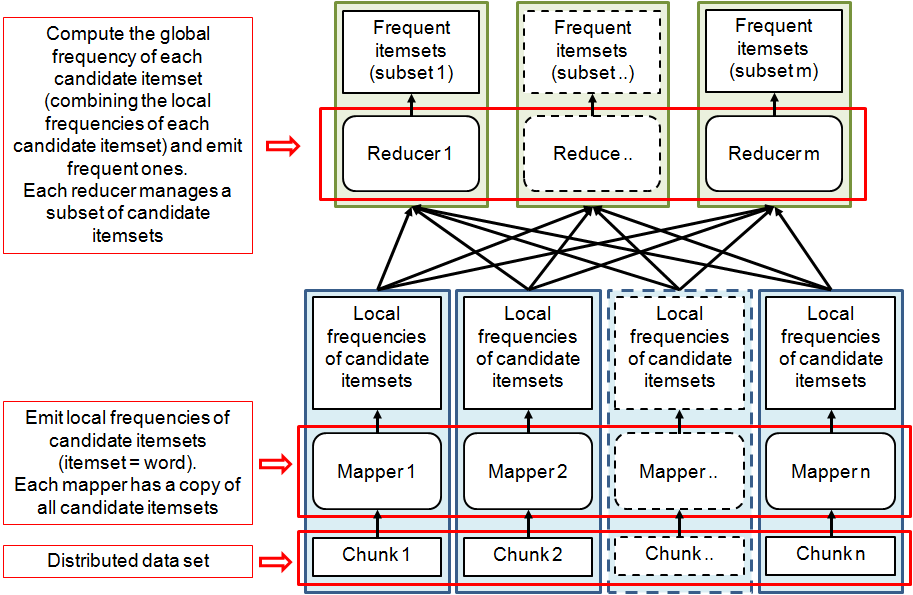
\includegraphics[width=5in]{immagini/Approach1noniterativo.eps}
\caption{Itemset mining parallelization: Data split approach}
\label{approach1noniterativo}
\end{figure}

\begin{figure}[!t]
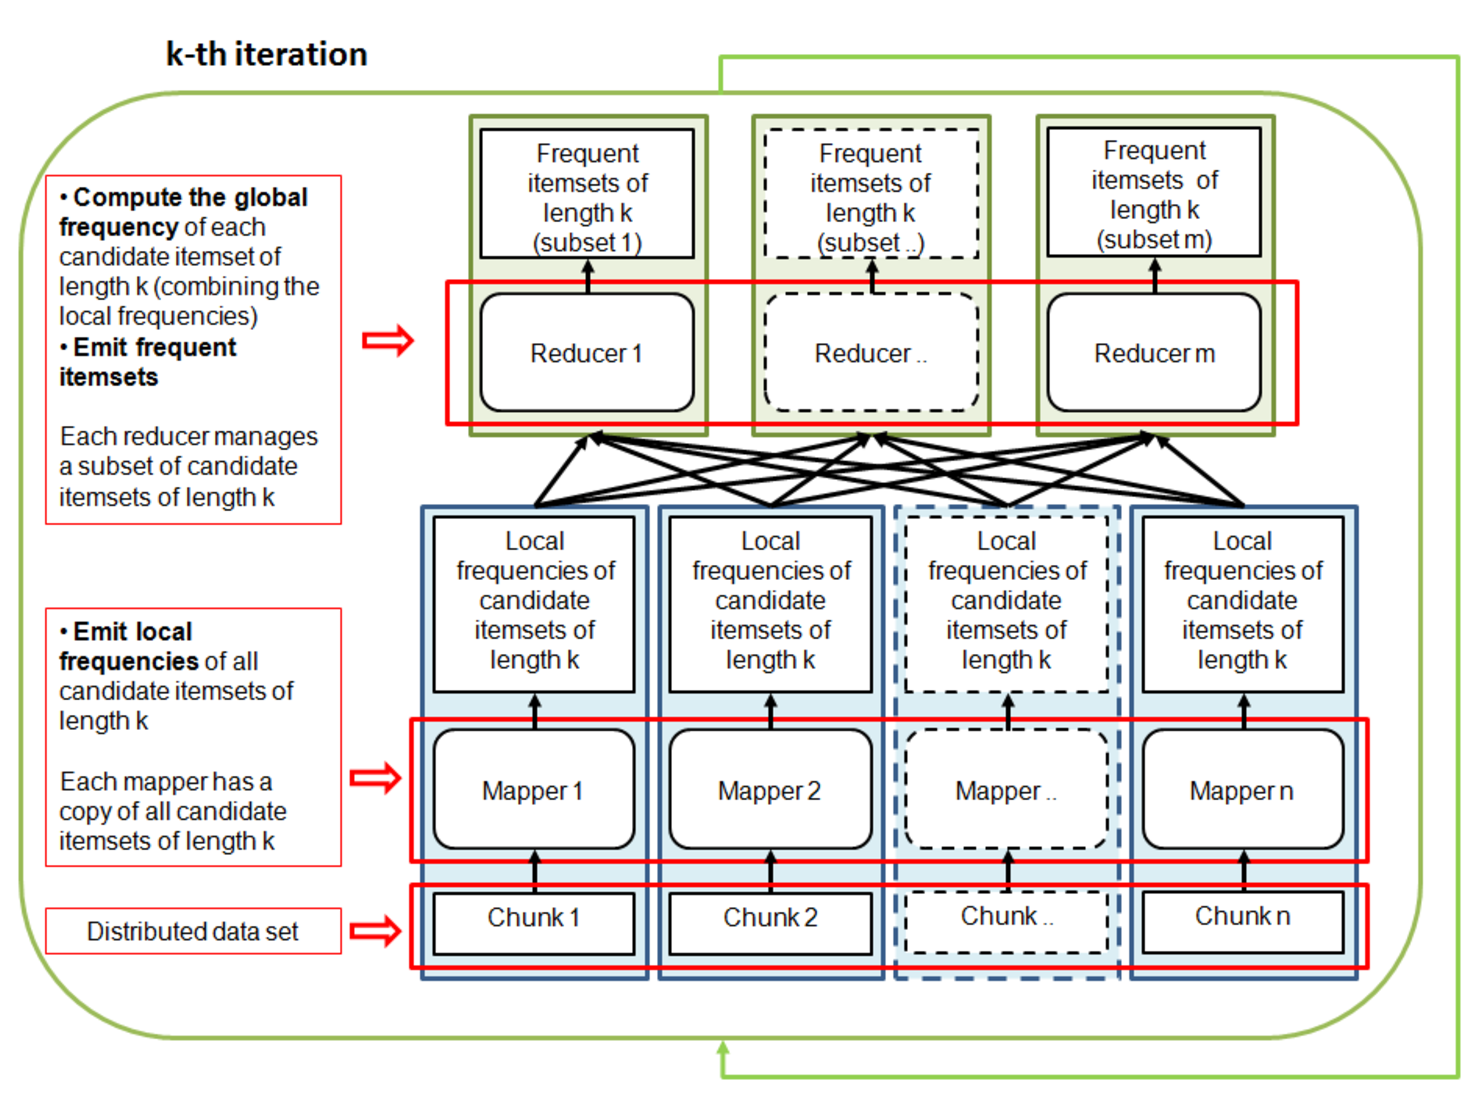
\includegraphics[width=5in]{immagini/Approach1.eps}
\caption{Itemset mining parallelization: Iterative Data split approach}
\label{approach1}
\end{figure}



\begin{figure}[!t]
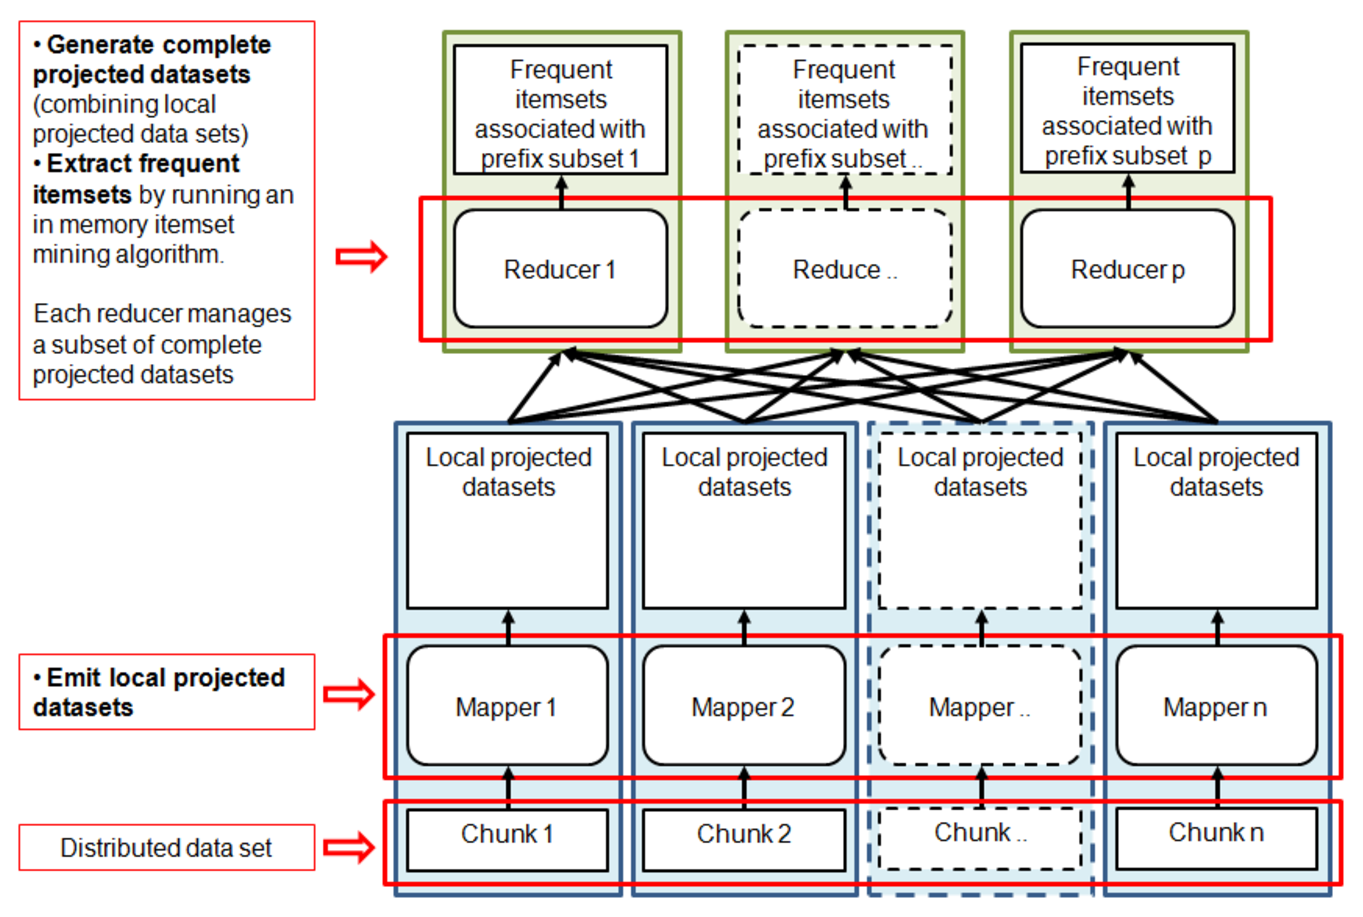
\includegraphics[width=5in]{immagini/Approach2.eps}
\caption{Itemset mining parallelization: Search space split approach}
\label{approach2}
\end{figure}


Figures~\ref{approach1noniterativo} and \ref{approach2} depict the first and the second parallelization strategies, respectively.  
In the data split approach (Figure~\ref{approach1noniterativo}), the map phase computes the local supports of the candidate itemsets in its data chunk  (i.e., each mapper runs a ``local itemset mining extraction'' on its data chunk). Then, the reduce phase merges the local supports of each candidate itemset to compute its global support. This solution requires each mapper to store a copy of the complete set of candidate itemsets (i.e., a copy of the lattice). 
This set must fit in the main memory of each mapper. Since the complete set of candidate itemsets is usually too large to be stored in the main memory of a single mapper, an iterative solution, inspired by the level-wise centralized itemset mining algorithms, is used. Figure~\ref{approach1} reports the iterative solution. 
At each iteration $k$ only the subset of candidates of length $k$ are considered and hence stored in the main memory of each mapper. This approach, thanks also to the exploitation of the apriori-principle to reduce the size of the candidate sets, allows obtaining subsets of candidate itemsets that can be loaded in the main memory of every mapper.

In the search space split approach (Figure~\ref{approach2}), the map phase generates a set of local projected datasets. Specifically each mapper generates a set of local projected datasets based on its data chunk. Each local projected dataset is the projection of the input chunk with respect to a prefix $p$.\footnote{Note that the projected datasets can overlap because the transactions associated with two distinct prefixes $p_1$ and $p_2$ can be overlapped.} Then, the reduce phase merges the local projected datasets to generate the complete projected datasets. Each complete projected dataset is provided as input to a standard centralized itemset mining algorithm running in the main memory of the reducer and the set of frequent itemsets associated to it are mined.
Each reducer is in charge of analyzing a subset of complete projected datasets by running the itemset mining phase on one complete projected dataset at a time.   
Hence, the main assumption, in this approach, is that each complete projected dataset must fit in the main memory of a single reducer. 

Table~\ref{tab:assumptions} summarizes the main characteristics of the two parallelization approaches with respect to the following criteria: 
type of split of the problem, 
usage of main memory, 
communication costs, 
load balancing, 
and maximum parallelization (i.e. maximum number of mappers and reducers).
%These are important issues to be addressed by distributed algorithms to increase their efficiency. 

%The communication cost is the amount of data sent on the network across the nodes of the cluster. The network can quickly  become the bottleneck 
%if large amount of data are sent on it. Hence, appropriate solutions must be adopted to limit it. 
%Load balancing is another important issue. It aims at assigning similar subproblems, characterized by similar execution times, to the nodes of the cluster to maximize the use of the available resources. A well-balanced application allows exploiting, simultaneously, all the available resources, whereas a non-well balanced applications is characterized by busy nodes (the ones associated with the longest tasks) and idle ones (the ones associated with the shortest tasks).

%For completeness, Table~\ref{tab:assumptions} reports both versions of Approach~1. However, the actual implementations are not based on the non-iterative version of Approach~1 because the complete set of itemsets (i.e., the complete lattice) is too large to be stored in main memory.


%\begin{table}[]
%\scriptsize
%\centering
%\caption{Comparison of the parallelization approaches.}\label{tab:assumptions}
%\begin{tabular}{|p{1.5cm}|p{3cm}|p{3cm}|p{3cm}|p{2cm}|}
%\hline {\bf Name} & {\bf Assumption} & {\bf Communication costs} & {\bf Load balancing} & {\bf Number of reads of the distributed dataset} \\
%\hline
%\hline Approach~1 (Figure~\ref{approach1noniterativo})& The complete set of candidate itemsets (i.e., the complete lattice) can be stored in the main memory of a single task. & Number of candidate itemsets $\times$ number of mappers. & Load balancing is achieved by associating the same number of itemsets to each reducer. & 1 \\
%
%\hline Approach~1 - Iterative version (Figure~\ref{approach1}) & Each candidate set of itemsets of length $k$ can be stored in the main memory of a single task. & Number of candidate itemsets $\times$ number of mappers $\times$ number of iterations. & Load balancing is achieved by associating the same number of itemsets to each reducer. & number of iterations (= size of the longest frequent itemset)\\
%\hline Approach~2 (Figure~\ref{approach2})& Each global projected dataset can be stored in the main memory of a single task. & Sum of the sizes of the local projected datasets. & Load balancing is not addressed. The tasks could be significantly unbalanced depending on the difference among the projected datasets and the related mining processes. & 1 \\
%\hline
%\end{tabular}
%\end{table}



\begin{table}[]
\scriptsize
\centering
\caption{Comparison of the parallelization approaches.}\label{tab:assumptions}
\begin{tabular}{|p{2.5cm}|p{5cm}|p{5cm}|}

\hline {\bf Criterion} & {\bf Iterative data split approach (Figure~\ref{approach1})} & {\bf Search space split approach (Figure~\ref{approach2})} \\
\hline
%\hline Type of split/Split of the search space &  All subproblems/mapper tasks analyze all the candidate itemsets of length $k$, but each one works on a different chunk of data. The final result is given by the merge of the local results.  &  Each subproblem analyzes a different subset of itemsets/a different part of the search space. The final result is the union of the local results. \\
\hline Type of split/Split of the search space &  Each subproblem analyzes a different subset of the input data and computes the local supports of 
all the candidate itemsets of length $k$ on its chunks of data. The final result is given by the merge of the local results.  &  Each subproblem analyzes a different subset of itemsets/a different part of the search space. The final result is the union of the local results. \\
\hline Usage of main memory &  The candidate set of length $k$ is stored in the main memory of a single task. & The complete projected dataset is stored in the main memory of a single task. \\
\hline Communication cost &  Number of candidate itemsets $\times$ number of mappers $\times$ number of iterations. & Sum of the sizes of the local projected datasets. \\
\hline Load balancing &  Load balancing is achieved by associating the same number of itemsets to each reducer. & The tasks could be significantly unbalanced depending on the characteristics of the projected datasets assigned to each node.\\
\hline Maximum number of mappers & Number of chunks  & Number of chunks  \\
\hline Maximum number of reducers & Number of candidate itemsets  & Number of items \\
\hline
\end{tabular}
\end{table}

%\begin{table}[]
%\scriptsize
%\centering
%\caption{Comparison of the parallelization approaches.}\label{tab:assumptions}
%\begin{tabular}{|p{2cm}|p{3.4cm}|p{3.4cm}|p{3.4cm}|}
%
%\hline {\bf Criterion} & {\bf Approach~1 (Figure~\ref{approach1noniterativo})} & {\bf Approach~1 - Iterative version (Figure~\ref{approach1})} & {\bf Approach~2 (Figure~\ref{approach2})} \\
%\hline
%\hline Type of split/Split of the search space & All subproblems/mapper tasks analyze all the candidate itemsets (i.e., work on the whole search space), but each one work on a different chunk of data. The final result is given by the merge of the local results.  & All subproblems/mapper tasks analyze all the candidate itemsets of length $k$, but each one work on a different chunk of data. The final result is given by the merge of the local results.  &  Each subproblem analyzes a different subset of itemsets/a different part of the search space. The final result if the union of the local results. \\
%\hline Use of the main memory & The complete set of candidate itemsets (i.e., the complete lattice) can be stored in the main memory of a single task.  &  Each candidate set of itemsets of length $k$ can be stored in the main memory of a single task. & Each global projected dataset can be stored in the main memory of a single task. \\
%\hline Communication costs & Number of candidate itemsets $\times$ number of mappers. &  Number of candidate itemsets $\times$ number of mappers $\times$ number of iterations. & Sum of the sizes of the local projected datasets. \\
%\hline Load balancing & Load balancing is achieved by associating the same number of itemsets to each reducer. &  Load balancing is achieved by associating the same number of itemsets to each reducer. & The tasks could be significantly unbalanced depending on the characteristics of the projected datasets assigned to each node and the related mining processes. Load balancing can not be easily achieved.\\
%%\hline Number of reads of the distributed dataset & 1 & Number of iterations (= size of the longest frequent itemset)  & 1 \\
%\hline Maximum number of mappers & Number of chunks & Number of chunks  & Number of chunks  \\
%\hline Maximum number of reducers & Number of candidate itemsets & Number of candidate itemsets  & Number of items \\
%\hline
%\end{tabular}
%\end{table}


\noindent{\bfseries Type of split/Split of the search space}. 
The main difference between the two parallelization approaches is the strategy adopted to split the problem in subproblems. This choice has a significant impact on the other criteria.

\noindent{\bfseries Usage of main memory}. 
The different usage of the main memory of the tasks impact on the reliability of the two approaches. The data split approach supposes that the candidate itemsets of length k can be stored in the main memory of each mapper. Hence, it is not able to scale on dense datasets
characterized by large candidate sets. Differently, the search space split approach supposes that each complete projected dataset can be stored in the main memory of a single task. Hence, this approach is not adequate, and runs out of memory, when large complete projected datasets are generated.  

\noindent{\bfseries Communication costs}. In a parallel MapReduce algorithm, communication costs are important since the network can easily become the bottleneck if large amounts of data are sent on the network.
The communication costs are mainly related to the outputs of the mappers which are sent to the reducers on the network. 
For the data split approach the data that is sent on the network is linear with respect 
to the number of candidate itemsets, the number of mappers, and the number of iterations.
Differently, for the search space approach, the amount of data emitted by the mappers is equal to the size of the projected datasets. 
%Since the projected datasets are overlapped the result is that the data sent across the network is potentially larger than the initial dataset\footnote{Usually, the size of the data sent on the network is not large as the initial dataset because compact trees are used to represent the projected datasets.}. 


\noindent{\bfseries Load balancing}. 
The different split of the problem in subproblems significantly impacts on load balancing. For the data split approach, the execution time of each mapper 
is linear with respect to the number of input transactions and the execution time of each reducer is linear with respect to the number of assigned itemsets.
Hence, the data split approach can easily achieve a good load balancing by assigning the same number of data chunks to each mapper and the same number of candidate itemsets to each reducer. 
Differently, the search space split approach is potentially unbalanced. In fact, each subproblem is associated with a different subset of the lattice, related to a specific projected dataset and prefix, and, depending on the data distribution, the complexity of the subproblems can significantly vary. 
A smart assignment of a set of subproblems to each node would mitigate the unbalance. However, the complexity of the subproblems is hardly inferable during the initial assignment phase.

\noindent{\bfseries Maximum number of mappers and reducers}. 
The two approaches are significantly different in terms of ``maximum parallelization degree'', at least in terms of number of maximum exploitable reducers. 
The maximum parallelization of the map phase is equal to the number of data chunks for both approaches.
% (i.e., maximum number of mappers = number of data chunks). 
Differently, the maximum parallelization of the reduce phase is equal to the number of candidate itemsets for the data split approach, because potentially each reducer could compute the global frequency of a single itemset, whereas it is equal to the number of global projected datasets for the second approach, which can be at most equal to the number of items. 
Since the number of candidate itemsets is greater than the number of items, the data split approach can potentially reach a higher degree of parallelization with respect to the search space split approach. 


%The communication costs are related to the outputs of the mappers. Since each mapper of the first approach emits one local support for each candidate itemset, the data that is sent on the network is linear with respect to the number of candidate itemsets and the number of mappers.
%Differently, for the second approach, the amount of data emitted by the mappers is equal to the size of the projected datasets. Since the projected datasets are overlapped the result is that the data sent across the network is potentially larger than the initial dataset\footnote{Usually, the size of the data sent on the network is not large as the initial dataset because compact trees are used to represent the projected datasets.}. 
%
%The different split of the problem in subproblems impacts also on load balancing. The first approach can easily achieve load balancing because all mappers perform the same operation and also all reducers perform the same operation. The only difference is given by the input data chunks and input candidate itemsets. By assigning the same number of data chunks to each mapper and the same number of candidate itemsets to each reducer, the result is that all mapper tasks are characterized by a similar execution time and also all reducers are characterized by a similar execution time. This means that the overall application is well-balanced. 
%Differently, the second approach is potentially unbalanced. In fact, each subproblem is associated with a different subspace of the search space, related to a specific projected dataset and prefix, and, depending on the data distribution, the complexity of the subproblems can significantly vary. A smart assignment of a set of subproblems to each node would mitigate the unbalance. However, the complexity of the subproblems is hardly inferable during the initial assignment phase.
%
%
%The two approaches are also different in terms of ``maximum parallelization degree'', at least in terms of number of maximum exploitable reducers. 
%The maximum parallelization of the map phase is equal to the number of data chunks for both approaches (i.e., maximum number of mappers = number of data chunks). Differently, the maximum parallelization of the reduce phase is equal to the number of candidate itemsets for the first approach, because potentially each reducer could compute the final frequency of a single itemset, whereas it is equal to the number of global projected datasets for the second approach, which can be at most 
%equal to the number of items. 
%Since the number of candidate itemsets is greater than the number of items, the first approach can reach a higher degree of parallelization with respect to the second approach. However, pay attention that a higher number of reducers corresponds also to a higher overhead related to the instantiation of the reducers. 

The two parallelization approaches are used to design efficient parallel implementations of well-known centralized itemset mining algorithms.  Specifically, the data split approach is used to implement the parallel versions of level-wise algorithms (like Apriori~\cite{apriori}), whereas the search space split approach is used to implement parallel versions of depth-first recursive approaches (like FP-growth~\cite{Han00} and Eclat~\cite{Zaki97newalgorithms}). 
%The map phase of the second approach can be seen as the first step of the recursion, that is used to generate the datasets projected with respect to prefixes composed of single items. Then, the reduce phase runs, in main memory, one instance of the mining algorithm for each projected dataset.




%{\bfseries Paolo: Capire cosa tenere della parte dopo che era la vecchia versione di questa sezione.}
%
%\textbf{Fabio: la metterei dopo l'intro degli algoritmi} In this section, we describe the main algorithmic solutions that have been exploited to address the
%parallelization of the itemset mining problem in the big data distributed environments (e.g., Hadoop and Spark).
%Many considerations are general and independent of the big data nature of the input data, whereas some other considerations and 
%algorithmic/design choices are driven by the big data characteristics of the input data (e.g., design of algorithms that exploit data locality).
%
%The parallelization and distributed execution of a generic algorithm, in the big data environment, is usually based on the split of the main task 
%in subtasks, each one working in isolation (shared-nothing) on one chunk of the data. However, this approach is not always possible and hence some algorithms 
%share small portions of data among the parallel tasks.
%
%The Hadoop-based algorithms usually parallelize the addressed problems by splitting the input datasets in independent data chucks. 
%Each chuck of the input data is assigned to a subtask that analyses the chunk of data in isolation (i.e., without needing the information 
%available in the other chunks). This is the map phase of the MapReduce programming paradigm. The outputs generated by the subtasks
%are then merged to obtain the final output (i.e., the output of the algorithm applied on the whole data). This second step is the reduce phase.
%The main assumptions of this solution are that (i) the input dataset is big (hence it cannot be sent on the network), whereas the outputs of 
%the subtasks are small and can be sent on the network and shared across the nodes of the cluster and (ii) the initial problem 
%can be split in subproblems each one working on one portion of the data and the portions are not overlapped.
%
%
%The algorithms that address the frequent itemset mining (FIM) \textbf{Fabio: FIM secondo me è piu' usato di FIMI} problem in the distributed environment can be grouped in two classes, based on how they split the problem: 
%\begin{enumerate}
%\item Data split approaches. These approaches parallelize the FIM problem by using the standard Hadoop-based approach, i.e., by splitting the data and assigning to each subtask one chunk.
%
%\item Search space split approaches. These approaches parallelize the FIM problem by splitting the search space, i.e., by assigning to each
% subtask the visit of a part of the  search space, even if this implies partial overlapping between the portions of data used by each subtask and 
% sending potentially large portions of the data on the network. 
%\end{enumerate}
%
%The algorithms of the first class exploit data locality, which is usually the most important point for the efficiency and scalability of 
%the MapReduce-based algorithms. However, when dealing with the itemset mining problem, 
%these solutions need to share common knowledge among the main memory 
%of the subtasks and the problem explodes when the amount of shared knowledge is larger than the main memory of each single task. Moreover, in this environment, they
%are iterative solutions that need to read multiple times the input dataset and this can be a problem when dealing with big data (the optimal solution
%should read only once the input dataset).
%
%%The algorithms belonging to the second class adopt a strategy that is not the ``standard'' one when the MapReduce programming paradigm is used,
%%because they are focused on the split of the search space and not on the split, without overlapping, of the input dataset.
%The algorithms belonging to the second class adopt a different strategy. While the MapReduce ``standard'' behavior assumes to split the input data in chunks and use them for the computation, in this case the search space is split in subproblems. Unfortunately, the result of this type of partitioning is that the input and the data structures of the obtained subproblems overlap. \textbf{Fabio: Dobbiamo introdurre meglio questo search space visto che ne parliamo cosi tanto}
%However,
%often these approaches are more efficient then the ones of the first class, especially when long patterns are mined (the longer the mined 
%patterns, the greater the number of times the input dataset is read when using the algorithms of the first class). 
%
%%Another important difference between the second class of algorithms and the first one is that the second class of algorithms 
%%aims at splitting the initial problem in subproblems that can be executed in ``main memory'', i.e., subproblems such that
%%the data of each subproblem can be stored in the main memory of one single task and a ``centralized' version of the mining problem can be 
%%executed in each task.
%
%Another important difference between the second class of algorithms and the first one is that such subproblems can be executed in  ``main memory''. In these cases, each subproblem is independent and is computed with a routine often inherited from a non-distributed frequent itemset mining algorithm.
%
%
%Among the 
%%available parallel big data itemset mining algorithms,
%considered algorithms
% YAFIM belongs to the first class while the two FP-Growth-based algorithms (i.e. Mahout and MLlib PFP) and DistEclat belong to the second class.
%BigFIM adopts a mixed approach (the first phase is related to the first class of algorithms and the second phase to the second class).  
%
%
%Another classification of the available algorithms is based on how they visit the search space. By using this criterion the algorithms can be classified in 
%two classes:
%\begin{enumerate}
%\item Breadth first approaches, also called level-wise approaches. These are iterative approaches that, at each iteration, visit a level of the 
%lattice of candidate itemsets/of the search space (i.e., at iteration $k$ mines the frequent itemset of length $k$).
%
%\item Depth first approaches. These approaches visit the search space by using a is a depth first strategy. 
%\end{enumerate}
%
%YAFIM belongs to the breadth first class, PFP and DistEclat belong to the Depth first approaches, while BigFIM uses a mixed approach (bread first for
%the mining of the itemset of length less than $k$ and depth first for the mining of the longer itemsets).
%\textbf{Fabio: non so se lo presenterei come due classificazione e poi associarle o direttamente come una sola perchè secondo me questi aspetti sono legatissimi}
%The groups of algorithms identified by the two classification criteria are the same because the breadth first approaches, for the itemset mining problem,
%fit well a parallelization based on the split of the input data, whereas the depth first approaches fix better a parallelization solution based on the 
%the split of the search space.
%
%



\section{Distributed itemset mining algorithms}
\label{algorithms}
%\begin{table}[]
%\scriptsize
%\centering
%\caption{Classification.}\label{tab:example1}
%\begin{tabular}{|c|c|c|c|c|c|}
%\hline 					& \multicolumn{5}{|c|}{\bf Distributed Algorithm/Implementation} \\
%\cline{2-6} {\bf Criterion} & {\bf Mahout PFP} & {\bf MLlib PFP} & {\bf Dist-Eclat} & {\bf BigFIM} & {\bf YAFIM} \\
%\hline
%\hline
%Search space & Depth First & Depth First & Depth First & Breadth First & Breadth First \\
%exploration  & & & & and  & \\
%strategy     & & & & Depth First & \\
%\hline
%Data  			  & Dense & Dense & Dense & Sparse & Sparse \\
%distribution	  & & & & and  &  \\
%				  & & & & dense  &  \\
%\hline
%Parallelization  & Search space & Search space & Search space & Data split & Data \\
%strategy         &  		& & & and  & split \\
%          &  		& & & Search space &  \\
%          &  		& & & split &  \\
%\hline
%Communication  & Yes & Yes & Yes & Yes  &  Yes  \\
%cost           & & & (trade-off & (trade-off &  \\
%handling       & & & with load & with load &  \\
%		       & & & balancing) & balancing) &  \\
%\hline
%Load balancing & No & No & Yes & Yes & No \\
%handling  & & & & &  \\
%\hline
%Framework  & Hadoop & Spark & Hadoop & Hadoop &  Spark  \\
%\hline
%Underlying centralized  & FP-Growth & FP-Growth & Eclat & Apiori &  Apriori \\
%algorithm  & & &  & and Eclat &  \\
%\hline
%\end{tabular}
%\end{table}



This section describes the algorithms, and available implementations, representing the state-of-the-art
solutions in the parallel frequent itemset mining context. We considered the following algorithms:
PFP~\cite{pfpgrowth},
BigFIM~\cite{bigfim}, DistEclat~\cite{bigfim},
and YAFIM~\cite{YAFIM}.
The only algorithm which is missing a publicly available implementation is YAFIM.
Among the considered algorithms, YAFIM belongs to the ones based on the data split approach discussed in Section~\ref{parallelization}, 
while the PFP and DistEclat are based on the search space split approach. Finally, BigFIM mixes the two strategies, aiming at exploiting the pros of them.
%The classification of the selected algorithms/implementations, based on the identified evaluation criteria, are summarized in Table~\ref{tab:example1}. 
For PFP we selected two popular implementations: Mahout PFP and MLlib PFP, which are based on Hadoop and Spark, respectively.  
The description of the four selected algorithms and their implementations are reported in the following subsections.

%\begin{table*}[]
%\scriptsize
%\centering
%\caption{Comparison summary. \textbf{Fabio: Aggiungere Parallelization!}\label{tab:example1}}
%\begin{tabular}{| c|c|c|c|c|c|c|}
%\hline {\bf Name} & {\bf Framework} & {\bf Underlying} & {\bf Data} & {\bf Search} & {\bf Comm.} & {\bf Load  }\\
%& & {\bf centralized} & {\bf distrib.} & {\bf strategy} & {\bf cost handling} & {\bf balance}\\
%& & {\bf algorithm} &&& & {\bf handling}\\
%\hline
%\hline Mahout PFP & Hadoop & FP-Growth & Dense & Depth First & Yes & No\\
%\hline MLlib PFP & Spark & FP-Growth & Dense & Depth First & Yes & No\\
%\hline Dist-Eclat & Hadoop & Eclat & Dense & Depth First & Yes & Yes \\
% &  &  &  &  & (trade-off with &  \\
% &  &  &  &  & load balancing) &  \\
%\hline BigFIM & Hadoop & Apriori and & Dense and  & Breadth First & Yes & Yes\\
%  &  & Eclat & sparse &  and &  (trade-off  with & \\
%   &  &  &  &Depth First  & load balancing) &  \\
%\hline YAFIM & Spark & Apriori & Sparse & Breadth First & Yes & No\\
%\hline
%\end{tabular}
%\end{table*}


%\begin{table}[]
%\scriptsize
%\centering
%\caption{Comparison summary.}\label{tab:example1}
%\begin{tabular}{|c|c|c|c|c|c|c|}
%\hline {\bf Name} & {\bf Framework} & {\bf Underlying} & {\bf Data} & {\bf Search} & {\bf Comm.} & {\bf Load  }\\
%& & {\bf centralized} & {\bf distrib.} & {\bf strategy} & {\bf cost} & {\bf balance}\\
%& & {\bf algorithm} &&& {\bf handling}& {\bf handling}\\
%\hline
%\hline Mahout PFP & Hadoop & FP-Growth & Dense & Depth First & Yes & No\\
%\hline MLlib PFP & Spark & FP-Growth & Dense & Depth First & Yes & No\\
%\hline Dist-Eclat & Hadoop & Eclat & Dense & Depth First & Yes & Yes \\
% &  &  &  &  & (trade-off with &  \\
% &  &  &  &  & load balancing) &  \\
%\hline BigFIM & Hadoop & Apriori and & Dense and  & Breadth First & Yes & Yes\\
%  &  & Eclat & sparse &  and &  (trade-off  with & \\
%   &  &  &  &Depth First  & load balancing) &  \\
%\hline YAFIM & Spark & Apriori & Sparse & Breadth First & Yes & No\\
%\hline
%\end{tabular}
%\end{table}


\subsection{YAFIM}
{\bf YAFIM}~\cite{YAFIM} is an Apriori distributed implementation developed in Spark.
%Apriori works well with sparse datasets and it is characterized by a different behavior with respect to Eclat and FP-growth: 
The iterative nature of the algorithm has always represented a challenge for its application in MapReduce-based Big Data
frameworks. The reasons are the overhead caused by the launch of new MapReduce
jobs and the requirement to read the input dataset from disk at each
iteration. YAFIM exploits Spark RDDs to cope with these issues. Precisely, it
assumes that all the dataset can be loaded into an RDD to speed up the
counting operations. Hence, after the first phase in which all the transactions
are loaded in an RDD, the algorithm starts the iterative Apriori algorithm organizing
the candidates in a hash tree to speed up the search.
Being strongly Apriori-based, it inherits the breadth-first strategy to explore and partition
the search space and the preference towards sparse data distributions.
YAFIM exploits the Spark ``broadcast variables abstraction'' feature, which allows
programmers to send subsets of shared data to each slave only once,
rather than with every job that uses those subset of data. This
implementation mitigates communication costs (reducing the inter job
communication), while load balancing is not addressed.

\subsection{Parallel FP-growth (PFP)}
\label{FP-Growth}
%FP-growth~\cite{Han00}, as mentioned, is among the most popular approaches for frequent pattern mining.
%It is based on a transposition of the
%whole dataset into a main memory compressed representation of the database
%called FP-tree. The algorithm is based on a recursive visit of the tree with a
%“divide and conquer”, partitioning-based approach. In the first phase the support of the items is
%counted to build the ``header table''. Then, the FP-tree is built exploiting the
%header table and the input dataset: each transaction is included adding or
%extending a path on the tree, exploiting common prefixes. Finally, for each
%item, it extracts the frequent itemsets from the item’s conditional FP-tree, in
%a recursive, depth first fashion. For the nature of the FP-tree, it is very robust to dense datasets. With a sparse dataset, the
%benefits of the FP-tree transposition would be reduced because there would be a
%higher number of branches and paths \cite{KumarBook} (i.e. a large number of
%subproblems to generate and results to merge).
%It is based on an FP-tree transposition of the transaction dataset and a
%recursive ``divide and conquer'' visit of the FP-tree. FP-Growth algorithm,
%instead, exploits a a main memory compressed representation of the database
%called FP-tree. The algorithm is based on a recursive visit of the tree with a
%``divide and conquer'' approach. FP-growth first phase consists of counting item
%support to build the header table. Then, the FP-tree is built exploiting the
%header table and the input dataset: each transaction is included adding or
%extending a path on the tree, exploiting common prefixes. Finally, for each
%item, it extracts the frequent itemsets from the item’s conditional FP-tree, in
%a recursive, depth first fashion.
{\bf Parallel FP-growth}~\cite{pfpgrowth}, called PFP, is a distributed implementation of FP-growth
that exploits the MapReduce paradigm to extract the $k$ most frequent closed
itemsets. It is included in the Mahout machine learning Library (version 0.9)
and it is developed on Apache Hadoop. 
PFP is based on the search space split parallelization strategy reported in Section~\ref{parallelization}. 
Specifically, the distributed algorithm is based on building independent FP-trees (i.e., projected datasets) that can be processed separately
over different nodes.

The algorithm consists of 3 MapReduce jobs.\\ 
\noindent{\it First job}. It builds the Header Table, that is used to select frequent items, in a MapReduce ``Word Count'' manner. \\
\noindent{\it Second job}. In the second job, the mappers project with respect to group of items (prefixes) all the transactions of the input dataset to generate the local projected contributions to the projected datasets. Then, the reducers aggregate the projections associated with the items of the same group and build independent complete FP-trees from them. Each complete FP-tree is managed by one reducer, which runs a local in main memory FP-growth algorithm on it and extracts the frequent itemsets associated with it.  \\
\noindent{\it Third job}. Finally, the last MapReduce job selects the top $k$ frequent closed itemsets.

The independent complete FP-trees can have different characteristics and this factor has
a significant impact on the execution time of the mining tasks. As discussed in Section~\ref{parallelization},
this factor significantly impacts on load balancing. Specifically,   
when the independent complete FP-trees have different sizes and characteristics, the tasks are unbalanced because they addresses
subproblems with different complexities. This problem could be potentially solved by
splitting complex trees in sub-trees, each one associated with an independent subproblem of the initial one.
However, defining a metric to split a tree
in such a way to obtain sub-mining problems that are equivalent in terms of execution time is not easy. In fact, the execution 
time of the itemset mining process on an FP-Tree is not only related to its size (number of nodes) but also to other characteristics (e.g., number of branches
and frequency of each node). 
Depending on the dataset characteristics, the communication costs can be very high, especially when the projected the datasets overlap significantly
because in that case the overlapping part of the data is sent multiple times on the network.

Spark PFP~\cite{MLLib} represents a pure transposition of PFP to Spark. It
is included in MLlib, the Spark machine learning library. The algorithm
implementation in Spark is very close to the Hadoop sibling. The main difference, in terms of addressed problem, is that 
MLlib PFP mines all the frequent itemsets, whereas Mahout PFP mines only the top $k$ closed itemsets. 
%It is characterized by dynamic and smooth
%handling of the different stages of the algorithm, without a strict division in
%phases. Its main advantage over the Hadoop sibling is the low I/O cost,
%potentially leading to a single read of the dataset from disk, by loading the
%transactions in an RDD and processing the data in main memory, whereas the
%Hadoop-based implementation of PFP performs many more I/O operations.

Both implementations, being strongly inspired by FP-growth, keep from the
underlying centralized algorithm the features related to the search space exploration
(depth-first) and the ability to efficiently mine itemsets from dense datasets.


\subsection{DistEclat and BigFIM}
\label{bigfim}
DistEclat~\cite{bigfim} is a Hadoop-based frequent itemset mining algorithms inspired 
by the Eclat algorithm, whereas BigFIM~\cite{bigfim} is a mixed two-phase algorithm that combines an Apriori-based approach with 
an Eclat-based one.

%Apriori~\cite{Agr94} is a very popular technique. It uses a bottom up approach
%in which frequent itemset are extended on item at a time (candidate generation)
%in a level-wise, breadth-first fashion, and groups of candidates are tested against the
%dataset. The search space is reduced through the downward-closure property,
%which guarantees that all the supersets of an infrequent itemset are infrequent
%too. Hence, each iteration consists of two steps: candidate generation and
%support count. The algorithm ends when no further frequent extension are found.
%
%%The data distribution which better fits Apriori is sparse. 
%For its algorithmic design, the Apriori algorithm is much affected by dataset density.
%In fact,
%with dense distribution the average transaction width can be very large, affecting
%the algorithms complexity. In this case, the candidates length starts to
%increase, increasing the number of candidates that should be generated, stored
%in main memory and tested. In general, Apriori is very efficient at
%the first steps, when the candidates are not long, but starts to be
%computationally intensive as soon as long candidates have to be kept in memory.

%The Eclat~\cite{Zaki97newalgorithms} algorithm performs the mining from a vertical
%transposition of the dataset: in this format, each transaction includes an item
%and the transaction identifiers ($tid$) in which it appears ($tidlist$).
%After the initial dataset
%transposition, the search space is explored in a depth-first manner similar to
%FP-growth. The algorithm is based on equivalence classes (groups of itemsets
%sharing a common prefix),  which are smartly merged to obtain all the
%candidates. Prefix-based equivalence classes are mined independently, in a ``divide and conquer' strategy', still
%taking advantage of downward closure property, even if the depth-first fashion
%of tree expansion reduces the pruning benefits. The support of a ($k+1$)-candidate
%is obtained intersecting the $tidlists$ of the $k$-itemsets from which it has been
%obtained, with no need of rescanning the whole dataset.
%
%Eclat architecture makes it robust to dense datasets: the depth-first search strategy may require
%more infrequent itemsets generated and tested than, for instance, Apriori does.
%As a result, Eclat efficiency reduces for sparse data with short patterns where
%most itemsets are infrequent~\cite{vu2012mining}.

{\bf DistEclat} is a frequent itemset miner developed on Apache Hadoop. It exploits
a parallel version of the Eclat algorithm to extract a superset of closed itemsets

The algorithm mainly consists of two steps. The first step extracts $k$-sized prefixes (i.e., frequent itemsets of length $k$) with respect to which, in
the second step, the algorithm builds independent projected subtrees, each one associated with an independent subproblem. Even in this case,
the main idea is to mine these independent trees in different nodes, exploiting the search split parallelization approach discussed in 
Section~\ref{parallelization}. 

The algorithm is organized in 3 MapReduce jobs. \\ 
\noindent{\it First job}. In the initial job, a MapReduce job transposes
the dataset into a vertical representation. \\
\noindent{\it Second job}. In this MapReduce job, each mapper extracts a subset of the $k$-sized prefixes ($k$-sized itemsets)
by running Eclat on the frequent items, and the related tidlists, assigned to it. The $k$-sized prefixes and the associated tidlists are then split in groups and assigned to the mappers of the last job.  \\
\noindent{\it Third job}. Each mapper of the last mapReduce job runs the in main memory version of Eclat 
on its set of independent prefixes. The final set of frequent itemsets is obtained by merging the outputs of the last job. 

The mining of the frequent itemsets in two different steps (i.e., mining of the itemsets of length $k$ in the second job and mining of the other frequent itemsets in the last job) aims at improving the load balancing of the algorithm. 
Specifically, the split in two steps allows obtaining simpler sub-problems, which are potentially characterized by similar execution times. Hence, the application is overall well-balanced.
%Specifically, the assignment of the $k$-sized prefixes before the last phase allows redistributing simplest sub-mining problems among the nodes of the cluster. Without this phase, more complex and unbalanced problems would be assigned to each node.

DistEclat is designed to be very fast but it assumes that all the tidlists of the frequent items should be stored in main memory.
In the worst case, each mapper needs the complete dataset, in vertical format, to build all the 2-prefixes~\cite{bigfim}. This impacts 
negatively on the scalability of DistEclat with respect to the dataset size.
The algorithm inherits from the centralized version the depth-first strategy to
explore the search space and the preference for dense datasets.

{\bf BigFIM} is an Hadoop-based solution very similar to DistEclat. 
Analogously to DistEclat, BigFIM is organized in two steps: (i) extraction of the frequent itemsets 
of length less than or equal to the input parameter $k$ and (ii) execution of Eclat on the sub-problems obtained splitting the search space with respect 
to the $k$-itemsets. The difference lies in the first step, where BigFIM exploits an Apriori-based algorithm to extract frequent $k$-itemsets, i.e., it adopts the data split parallelization approach (Section~\ref{parallelization}). 
Even if BigFIM is slower than DistEclat, BigFIM is designed to run on larger datasets.
%In fact, the parallel Apriori-based algorithm used by BigFIM, based on the first parallelization strategy introduced in Section~\ref{parallelization}, 
%scales with respect to the number of transactions of the dataset. 
%However, it supposes that the candidate $k$-sized itemsets can be store in main memory. 
%Hence, it scales with respect to the number of transactions but not with respect to the number of candidate itemsets and can incur in out of memory problems with dense datasets. 
The reason is related to the first step in which, exploiting an Apriori-based approach,
the $k$-prefixes are extracted in a breadth-first fashion.  Consequently, the nodes do not have to keep large tidlists in main memory but only the set of candidate itemsets to be counted. However, this is also the most critical issue of the application of the data split parallelization approach, because, depending on the dataset density, the set of candidate itemsets may not be stored in main memory. 

Because of the two different techniques used by BigFIM in its two main steps (data split and then search space split), 
in the first step BigFIM achieves the best performance with sparse datasets, while in the second phase it better fits dense data distributions.
%: overall it does not show a data-distribution preference.

DistEclat and BigFIM are the only algorithms specifically designed for addressing 
load balancing and communication cost by means of the prefix length parameter $k$. 
In particular, the choice of the length of the prefixes
generated during the first step affects both load
balancing and communication cost. The former would
improve with a deeper level of the mining phase before the redistribution of the
prefixes while the latter would benefit from shorter prefixes. 
Hence, depending on the data distribution and the characteristics of the
Hadoop cluster, DistEclat and BigFIM can be tuned to optimize load balancing and communication
cost.
% BigFIM and DistEclat require additional inputs besides the minsup (Minimum Support),
% since they work with a customizable length of first-phase prefixes,
% and this feature could require some iterations to find
% the best value, depending on the kind of datasets and the cluster configuration.
% Tuning the prefix length allows BigFIM and DistEclat to handle both
% communication costs and load balancing.




%\begin{table*}[]
%\scriptsize
%\centering
%\caption{Algorithm analysis \label{tab:example1}}
%\begin{tabular}{| c|c|c|c|c|c|c|}
%\hline {\bf Name} & {\bf Framework} & {\bf Underlying algorithm} & {\bf Data distribution} & {\bf Search Strategy} & {\bf Communication cost handling} & {\bf Load balance handling }\\
%
%%\hline {\bf Name} & {\bf Framework} & {\bf Underlying} & {\bf Data} & {\bf Search} & {\bf Communication} & {\bf Load  }\\
%%& & {\bf algorithm} & {\bf distribution} & {\bf Strategy} & {\bf cost handling} & {\bf balance}\\
%%& & &&& & {\bf handling}\\
%\hline
%\hline PFP & Hadoop & FP-Growth & dense & Depth First & Yes & No\\
%\hline Spark PFP & Spark & FP-Growth & dense & Depth First & Yes & No\\
%\hline DistEclat & Hadoop & Eclat & dense & Depth First &  Yes (best effort withload balancing) & Yes \\
%
%\hline BigFIM & Hadoop & Apriori and  Eclat& Dense and Sparse & Breadth First and& Yes (best effort withload balancing)& Yes\\
% &&  &  &  Depth First & & \\
%\hline YAFIM & Spark & Apriori & sparse & Breadth First & Yes & No\\
%\hline
%\end{tabular}
%\end{table*}




\section{Selected algorithms}
\label{algorithms}
%\begin{table}[]
%\scriptsize
%\centering
%\caption{Classification.}\label{tab:example1}
%\begin{tabular}{|c|c|c|c|c|c|}
%\hline 					& \multicolumn{5}{|c|}{\bf Distributed Algorithm/Implementation} \\
%\cline{2-6} {\bf Criterion} & {\bf Mahout PFP} & {\bf MLlib PFP} & {\bf Dist-Eclat} & {\bf BigFIM} & {\bf YAFIM} \\
%\hline
%\hline
%Search space & Depth First & Depth First & Depth First & Breadth First & Breadth First \\
%exploration  & & & & and  & \\
%strategy     & & & & Depth First & \\
%\hline
%Data  			  & Dense & Dense & Dense & Sparse & Sparse \\
%distribution	  & & & & and  &  \\
%				  & & & & dense  &  \\
%\hline
%Parallelization  & Search space & Search space & Search space & Data split & Data \\
%strategy         &  		& & & and  & split \\
%          &  		& & & Search space &  \\
%          &  		& & & split &  \\
%\hline
%Communication  & Yes & Yes & Yes & Yes  &  Yes  \\
%cost           & & & (trade-off & (trade-off &  \\
%handling       & & & with load & with load &  \\
%		       & & & balancing) & balancing) &  \\
%\hline
%Load balancing & No & No & Yes & Yes & No \\
%handling  & & & & &  \\
%\hline
%Framework  & Hadoop & Spark & Hadoop & Hadoop &  Spark  \\
%\hline
%Underlying centralized  & FP-Growth & FP-Growth & Eclat & Apiori &  Apriori \\
%algorithm  & & &  & and Eclat &  \\
%\hline
%\end{tabular}
%\end{table}



This section describes the algorithms, and available implementations, representing the state-of-the-art
solutions in the parallel frequent itemset mining context. We considered the following algorithms:
PFP~\cite{pfpgrowth},
BigFIM~\cite{bigfim}, DistEclat~\cite{bigfim},
and YAFIM~\cite{YAFIM}.
The only algorithm which is missing a publicly available implementation is YAFIM.
Among the considered algorithms, YAFIM belongs to the ones based on the data split approach discussed in Section~\ref{parallelization}, 
while the PFP and DistEclat are based on the search space split approach. Finally, BigFIM mixes the two strategies, aiming at exploiting the pros of them.
%The classification of the selected algorithms/implementations, based on the identified evaluation criteria, are summarized in Table~\ref{tab:example1}. 
For PFP we selected two popular implementations: Mahout PFP and MLlib PFP, which are based on Hadoop and Spark, respectively.  
The description of the four selected algorithms and their implementations are reported in the following subsections.

%\begin{table*}[]
%\scriptsize
%\centering
%\caption{Comparison summary. \textbf{Fabio: Aggiungere Parallelization!}\label{tab:example1}}
%\begin{tabular}{| c|c|c|c|c|c|c|}
%\hline {\bf Name} & {\bf Framework} & {\bf Underlying} & {\bf Data} & {\bf Search} & {\bf Comm.} & {\bf Load  }\\
%& & {\bf centralized} & {\bf distrib.} & {\bf strategy} & {\bf cost handling} & {\bf balance}\\
%& & {\bf algorithm} &&& & {\bf handling}\\
%\hline
%\hline Mahout PFP & Hadoop & FP-Growth & Dense & Depth First & Yes & No\\
%\hline MLlib PFP & Spark & FP-Growth & Dense & Depth First & Yes & No\\
%\hline Dist-Eclat & Hadoop & Eclat & Dense & Depth First & Yes & Yes \\
% &  &  &  &  & (trade-off with &  \\
% &  &  &  &  & load balancing) &  \\
%\hline BigFIM & Hadoop & Apriori and & Dense and  & Breadth First & Yes & Yes\\
%  &  & Eclat & sparse &  and &  (trade-off  with & \\
%   &  &  &  &Depth First  & load balancing) &  \\
%\hline YAFIM & Spark & Apriori & Sparse & Breadth First & Yes & No\\
%\hline
%\end{tabular}
%\end{table*}


%\begin{table}[]
%\scriptsize
%\centering
%\caption{Comparison summary.}\label{tab:example1}
%\begin{tabular}{|c|c|c|c|c|c|c|}
%\hline {\bf Name} & {\bf Framework} & {\bf Underlying} & {\bf Data} & {\bf Search} & {\bf Comm.} & {\bf Load  }\\
%& & {\bf centralized} & {\bf distrib.} & {\bf strategy} & {\bf cost} & {\bf balance}\\
%& & {\bf algorithm} &&& {\bf handling}& {\bf handling}\\
%\hline
%\hline Mahout PFP & Hadoop & FP-Growth & Dense & Depth First & Yes & No\\
%\hline MLlib PFP & Spark & FP-Growth & Dense & Depth First & Yes & No\\
%\hline Dist-Eclat & Hadoop & Eclat & Dense & Depth First & Yes & Yes \\
% &  &  &  &  & (trade-off with &  \\
% &  &  &  &  & load balancing) &  \\
%\hline BigFIM & Hadoop & Apriori and & Dense and  & Breadth First & Yes & Yes\\
%  &  & Eclat & sparse &  and &  (trade-off  with & \\
%   &  &  &  &Depth First  & load balancing) &  \\
%\hline YAFIM & Spark & Apriori & Sparse & Breadth First & Yes & No\\
%\hline
%\end{tabular}
%\end{table}


\subsection{YAFIM}
{\bf YAFIM}~\cite{YAFIM} is an Apriori distributed implementation developed in Spark.
%Apriori works well with sparse datasets and it is characterized by a different behavior with respect to Eclat and FP-growth: 
The iterative nature of the algorithm has always represented a challenge for its application in MapReduce-based Big Data
frameworks. The reasons are the overhead caused by the launch of new MapReduce
jobs and the requirement to read the input dataset from disk at each
iteration. YAFIM exploits Spark RDDs to cope with these issues. Precisely, it
assumes that all the dataset can be loaded into an RDD to speed up the
counting operations. Hence, after the first phase in which all the transactions
are loaded in an RDD, the algorithm starts the iterative Apriori algorithm organizing
the candidates in a hash tree to speed up the search.
Being strongly Apriori-based, it inherits the breadth-first strategy to explore and partition
the search space and the preference towards sparse data distributions.
YAFIM exploits the Spark ``broadcast variables abstraction'' feature, which allows
programmers to send subsets of shared data to each slave only once,
rather than with every job that uses those subset of data. This
implementation mitigates communication costs (reducing the inter job
communication), while load balancing is not addressed.

\subsection{Parallel FP-growth (PFP)}
\label{FP-Growth}
%FP-growth~\cite{Han00}, as mentioned, is among the most popular approaches for frequent pattern mining.
%It is based on a transposition of the
%whole dataset into a main memory compressed representation of the database
%called FP-tree. The algorithm is based on a recursive visit of the tree with a
%“divide and conquer”, partitioning-based approach. In the first phase the support of the items is
%counted to build the ``header table''. Then, the FP-tree is built exploiting the
%header table and the input dataset: each transaction is included adding or
%extending a path on the tree, exploiting common prefixes. Finally, for each
%item, it extracts the frequent itemsets from the item’s conditional FP-tree, in
%a recursive, depth first fashion. For the nature of the FP-tree, it is very robust to dense datasets. With a sparse dataset, the
%benefits of the FP-tree transposition would be reduced because there would be a
%higher number of branches and paths \cite{KumarBook} (i.e. a large number of
%subproblems to generate and results to merge).
%It is based on an FP-tree transposition of the transaction dataset and a
%recursive ``divide and conquer'' visit of the FP-tree. FP-Growth algorithm,
%instead, exploits a a main memory compressed representation of the database
%called FP-tree. The algorithm is based on a recursive visit of the tree with a
%``divide and conquer'' approach. FP-growth first phase consists of counting item
%support to build the header table. Then, the FP-tree is built exploiting the
%header table and the input dataset: each transaction is included adding or
%extending a path on the tree, exploiting common prefixes. Finally, for each
%item, it extracts the frequent itemsets from the item’s conditional FP-tree, in
%a recursive, depth first fashion.
{\bf Parallel FP-growth}~\cite{pfpgrowth}, called PFP, is a distributed implementation of FP-growth
that exploits the MapReduce paradigm to extract the $k$ most frequent closed
itemsets. It is included in the Mahout machine learning Library (version 0.9)
and it is developed on Apache Hadoop. 
PFP is based on the search space split parallelization strategy reported in Section~\ref{parallelization}. 
Specifically, the distributed algorithm is based on building independent FP-trees (i.e., projected datasets) that can be processed separately
over different nodes.

The algorithm consists of 3 MapReduce jobs.\\ 
\noindent{\it First job}. It builds the Header Table, that is used to select frequent items, in a MapReduce ``Word Count'' manner. \\
\noindent{\it Second job}. In the second job, the mappers project with respect to group of items (prefixes) all the transactions of the input dataset to generate the local projected contributions to the projected datasets. Then, the reducers aggregate the projections associated with the items of the same group and build independent complete FP-trees from them. Each complete FP-tree is managed by one reducer, which runs a local in main memory FP-growth algorithm on it and extracts the frequent itemsets associated with it.  \\
\noindent{\it Third job}. Finally, the last MapReduce job selects the top $k$ frequent closed itemsets.

The independent complete FP-trees can have different characteristics and this factor has
a significant impact on the execution time of the mining tasks. As discussed in Section~\ref{parallelization},
this factor significantly impacts on load balancing. Specifically,   
when the independent complete FP-trees have different sizes and characteristics, the tasks are unbalanced because they addresses
subproblems with different complexities. This problem could be potentially solved by
splitting complex trees in sub-trees, each one associated with an independent subproblem of the initial one.
However, defining a metric to split a tree
in such a way to obtain sub-mining problems that are equivalent in terms of execution time is not easy. In fact, the execution 
time of the itemset mining process on an FP-Tree is not only related to its size (number of nodes) but also to other characteristics (e.g., number of branches
and frequency of each node). 
Depending on the dataset characteristics, the communication costs can be very high, especially when the projected the datasets overlap significantly
because in that case the overlapping part of the data is sent multiple times on the network.

Spark PFP~\cite{MLLib} represents a pure transposition of PFP to Spark. It
is included in MLlib, the Spark machine learning library. The algorithm
implementation in Spark is very close to the Hadoop sibling. The main difference, in terms of addressed problem, is that 
MLlib PFP mines all the frequent itemsets, whereas Mahout PFP mines only the top $k$ closed itemsets. 
%It is characterized by dynamic and smooth
%handling of the different stages of the algorithm, without a strict division in
%phases. Its main advantage over the Hadoop sibling is the low I/O cost,
%potentially leading to a single read of the dataset from disk, by loading the
%transactions in an RDD and processing the data in main memory, whereas the
%Hadoop-based implementation of PFP performs many more I/O operations.

Both implementations, being strongly inspired by FP-growth, keep from the
underlying centralized algorithm the features related to the search space exploration
(depth-first) and the ability to efficiently mine itemsets from dense datasets.


\subsection{DistEclat and BigFIM}
\label{bigfim}
DistEclat~\cite{bigfim} is a Hadoop-based frequent itemset mining algorithms inspired 
by the Eclat algorithm, whereas BigFIM~\cite{bigfim} is a mixed two-phase algorithm that combines an Apriori-based approach with 
an Eclat-based one.

%Apriori~\cite{Agr94} is a very popular technique. It uses a bottom up approach
%in which frequent itemset are extended on item at a time (candidate generation)
%in a level-wise, breadth-first fashion, and groups of candidates are tested against the
%dataset. The search space is reduced through the downward-closure property,
%which guarantees that all the supersets of an infrequent itemset are infrequent
%too. Hence, each iteration consists of two steps: candidate generation and
%support count. The algorithm ends when no further frequent extension are found.
%
%%The data distribution which better fits Apriori is sparse. 
%For its algorithmic design, the Apriori algorithm is much affected by dataset density.
%In fact,
%with dense distribution the average transaction width can be very large, affecting
%the algorithms complexity. In this case, the candidates length starts to
%increase, increasing the number of candidates that should be generated, stored
%in main memory and tested. In general, Apriori is very efficient at
%the first steps, when the candidates are not long, but starts to be
%computationally intensive as soon as long candidates have to be kept in memory.

%The Eclat~\cite{Zaki97newalgorithms} algorithm performs the mining from a vertical
%transposition of the dataset: in this format, each transaction includes an item
%and the transaction identifiers ($tid$) in which it appears ($tidlist$).
%After the initial dataset
%transposition, the search space is explored in a depth-first manner similar to
%FP-growth. The algorithm is based on equivalence classes (groups of itemsets
%sharing a common prefix),  which are smartly merged to obtain all the
%candidates. Prefix-based equivalence classes are mined independently, in a ``divide and conquer' strategy', still
%taking advantage of downward closure property, even if the depth-first fashion
%of tree expansion reduces the pruning benefits. The support of a ($k+1$)-candidate
%is obtained intersecting the $tidlists$ of the $k$-itemsets from which it has been
%obtained, with no need of rescanning the whole dataset.
%
%Eclat architecture makes it robust to dense datasets: the depth-first search strategy may require
%more infrequent itemsets generated and tested than, for instance, Apriori does.
%As a result, Eclat efficiency reduces for sparse data with short patterns where
%most itemsets are infrequent~\cite{vu2012mining}.

{\bf DistEclat} is a frequent itemset miner developed on Apache Hadoop. It exploits
a parallel version of the Eclat algorithm to extract a superset of closed itemsets

The algorithm mainly consists of two steps. The first step extracts $k$-sized prefixes (i.e., frequent itemsets of length $k$) with respect to which, in
the second step, the algorithm builds independent projected subtrees, each one associated with an independent subproblem. Even in this case,
the main idea is to mine these independent trees in different nodes, exploiting the search split parallelization approach discussed in 
Section~\ref{parallelization}. 

The algorithm is organized in 3 MapReduce jobs. \\ 
\noindent{\it First job}. In the initial job, a MapReduce job transposes
the dataset into a vertical representation. \\
\noindent{\it Second job}. In this MapReduce job, each mapper extracts a subset of the $k$-sized prefixes ($k$-sized itemsets)
by running Eclat on the frequent items, and the related tidlists, assigned to it. The $k$-sized prefixes and the associated tidlists are then split in groups and assigned to the mappers of the last job.  \\
\noindent{\it Third job}. Each mapper of the last mapReduce job runs the in main memory version of Eclat 
on its set of independent prefixes. The final set of frequent itemsets is obtained by merging the outputs of the last job. 

The mining of the frequent itemsets in two different steps (i.e., mining of the itemsets of length $k$ in the second job and mining of the other frequent itemsets in the last job) aims at improving the load balancing of the algorithm. 
Specifically, the split in two steps allows obtaining simpler sub-problems, which are potentially characterized by similar execution times. Hence, the application is overall well-balanced.
%Specifically, the assignment of the $k$-sized prefixes before the last phase allows redistributing simplest sub-mining problems among the nodes of the cluster. Without this phase, more complex and unbalanced problems would be assigned to each node.

DistEclat is designed to be very fast but it assumes that all the tidlists of the frequent items should be stored in main memory.
In the worst case, each mapper needs the complete dataset, in vertical format, to build all the 2-prefixes~\cite{bigfim}. This impacts 
negatively on the scalability of DistEclat with respect to the dataset size.
The algorithm inherits from the centralized version the depth-first strategy to
explore the search space and the preference for dense datasets.

{\bf BigFIM} is an Hadoop-based solution very similar to DistEclat. 
Analogously to DistEclat, BigFIM is organized in two steps: (i) extraction of the frequent itemsets 
of length less than or equal to the input parameter $k$ and (ii) execution of Eclat on the sub-problems obtained splitting the search space with respect 
to the $k$-itemsets. The difference lies in the first step, where BigFIM exploits an Apriori-based algorithm to extract frequent $k$-itemsets, i.e., it adopts the data split parallelization approach (Section~\ref{parallelization}). 
Even if BigFIM is slower than DistEclat, BigFIM is designed to run on larger datasets.
%In fact, the parallel Apriori-based algorithm used by BigFIM, based on the first parallelization strategy introduced in Section~\ref{parallelization}, 
%scales with respect to the number of transactions of the dataset. 
%However, it supposes that the candidate $k$-sized itemsets can be store in main memory. 
%Hence, it scales with respect to the number of transactions but not with respect to the number of candidate itemsets and can incur in out of memory problems with dense datasets. 
The reason is related to the first step in which, exploiting an Apriori-based approach,
the $k$-prefixes are extracted in a breadth-first fashion.  Consequently, the nodes do not have to keep large tidlists in main memory but only the set of candidate itemsets to be counted. However, this is also the most critical issue of the application of the data split parallelization approach, because, depending on the dataset density, the set of candidate itemsets may not be stored in main memory. 

Because of the two different techniques used by BigFIM in its two main steps (data split and then search space split), 
in the first step BigFIM achieves the best performance with sparse datasets, while in the second phase it better fits dense data distributions.
%: overall it does not show a data-distribution preference.

DistEclat and BigFIM are the only algorithms specifically designed for addressing 
load balancing and communication cost by means of the prefix length parameter $k$. 
In particular, the choice of the length of the prefixes
generated during the first step affects both load
balancing and communication cost. The former would
improve with a deeper level of the mining phase before the redistribution of the
prefixes while the latter would benefit from shorter prefixes. 
Hence, depending on the data distribution and the characteristics of the
Hadoop cluster, DistEclat and BigFIM can be tuned to optimize load balancing and communication
cost.
% BigFIM and DistEclat require additional inputs besides the minsup (Minimum Support),
% since they work with a customizable length of first-phase prefixes,
% and this feature could require some iterations to find
% the best value, depending on the kind of datasets and the cluster configuration.
% Tuning the prefix length allows BigFIM and DistEclat to handle both
% communication costs and load balancing.




%\begin{table*}[]
%\scriptsize
%\centering
%\caption{Algorithm analysis \label{tab:example1}}
%\begin{tabular}{| c|c|c|c|c|c|c|}
%\hline {\bf Name} & {\bf Framework} & {\bf Underlying algorithm} & {\bf Data distribution} & {\bf Search Strategy} & {\bf Communication cost handling} & {\bf Load balance handling }\\
%
%%\hline {\bf Name} & {\bf Framework} & {\bf Underlying} & {\bf Data} & {\bf Search} & {\bf Communication} & {\bf Load  }\\
%%& & {\bf algorithm} & {\bf distribution} & {\bf Strategy} & {\bf cost handling} & {\bf balance}\\
%%& & &&& & {\bf handling}\\
%\hline
%\hline PFP & Hadoop & FP-Growth & dense & Depth First & Yes & No\\
%\hline Spark PFP & Spark & FP-Growth & dense & Depth First & Yes & No\\
%\hline DistEclat & Hadoop & Eclat & dense & Depth First &  Yes (best effort withload balancing) & Yes \\
%
%\hline BigFIM & Hadoop & Apriori and  Eclat& Dense and Sparse & Breadth First and& Yes (best effort withload balancing)& Yes\\
% &&  &  &  Depth First & & \\
%\hline YAFIM & Spark & Apriori & sparse & Breadth First & Yes & No\\
%\hline
%\end{tabular}
%\end{table*}






\section{Experimental evaluation}
\label{experimental}

In this section, the results of the experimental comparison are presented.
The purpose of the experiments is to compare the behaviours of the algorithms
and their distributed implementations,
by considering  different data distributions and use cases, and to highlight
pros and cons of each algorithm.
Specifically, experiments analyze the algorithms in terms of
(i)~efficiency (i.e., execution time) under different conditions
(Sections~\ref{minsup_exp}-\ref{usecases}),
(ii)~load balancing (Section~\ref{load_exp}), and
(iii)~communication costs (Section~\ref{communication_costs}).
Finally, Section~\ref{lesson} presents a summary of the ``lessons learned''.
%by providing some hints about the most suitable algorithm(s) depending
%on the use case/data distribution.

% %The frequent itemset mining domain is very complex and there are many factors
% which impact the efficiency of the mining process.
% %The data distribution of the input data set (i.e., the number of transactions
% and the average transaction length) is only one of the features affecting the
% mining, especially in real life use cases.
% %For this reason, we have tested the approaches on a set of both synthetic and
% real datasets. The first type of experiments consists on measuring the execution
% time of the mining process with different minimum support thresholds values. The
% second set evaluates the performance of the algorithms dealing with datasets of
% different average transaction length. The third set of experiments are obtained
% processing datasets with different length of expected frequent patterns while
% the forth is related to a different number of transactions.
% % %After these experiments, we evaluated the approaches in a real life use case,
% % dealing with a real web tags dataset and extracting the most frequent patterns
% % on an incremental time period. Finally, all the approaches are evaluated
% % analysing the load balance and the communication cost on the different tasks.

We evaluated the implementations of four of the algorithms described
in Section~\ref{algorithms}.
Specifically, we considered
the Parallel FP-Growth implementations
of Mahout 0.9 (called Mahout PFP)~\cite{Mahout}
and MLlib for Spark 1.3.0 (called MLlib PFP)~\cite{MLLib},
the June 2015 implementation of BigFIM~\cite{Bigfim_github},
and the version of DistEclat downloaded from \cite{Bigfim_github}
on September 2015.
Unfortunately, the implementation of the YAFIM algorithm is not available.
Therefore, YAFIM is not included in this experimental comparison.

% %The Parallel FP-Growth implementations are the ones delivered along with Mahout
% 0.9 and Apache MLlib of Spark 1.3.0, respectively based on Apache Hadoop and
% Apache Spark. Specifically, while the Mahout algorithm is ready to be used
% off-the-shelf, the Parallel FP-growth Spark implementation is not a stand alone
% class. The BigFIM benchmarks are obtained with the implementation of June 2015
% while the DistEclat experiments are executed with the implementation of
% September 2015. Unfortunately, the Apriori based algorithm YAFIM is not
% available. Therefore, YAFIM is not included in this experimental comparison.

We recall that Mahout PFP extracts the top $k$ frequent closed itemsets, BigFIM
and DistEclat extract a superset of the frequent closed itemsets,
while MLlib PFP extracts all the frequent itemsets.
To perform a fair comparison, Mahout PFP is forced to output all the closed
itemsets.
Since the extraction of the complete set of frequent itemsets is usually
more resource intensive than dealing with only the set of frequent closed
itemsets\footnote{We recall that the complete set of frequent itemsets can be
obtained expanding and combining the closed itemsets by means of a
post-processing step.},
the execution times of Mahout PFP, BigFIM and DistEclat may increase with respect
to MLlib PFP.
In our experiments, we took care to verify that
the numbers of frequent itemsets and closed itemsets are the same.
Therefore, the disadvantages related to the more intensive task performed
by MLlib are mitigated.
%However, for all the performed experiments, the number of frequent itemsets and
%closed itemsets is so similar that the
%difference is negligible and it does not affect our results.
% Hence, the disadvantages related to the more
%intensive task performed by MLlib PFP are irrelevant.



%The extraction of all the frequent itemsets usually is more resource intensive
%than dealing with only the frequent closed ones. The formers can be obtained
%expanding and combining the latters. For these reason, the reader should take
%into account that, in order to obtain the same output (i.e. the complete set of
%frequent closed itemsets), the current execution times of Mahout PFP, BigFIM and
%DistEclat can only increase. However, this issue, as highlighted in the next
%subsection, is strongly mitigated by the utilization of a more modern framework
%such as Spark.

We defined a common set of default parameter values for all experiments,
different settings are explicitly indicated.
The default setting of each algorithm was chosen by taking into consideration
the physical characteristics of the Hadoop cluster,
to allow each approach to exploit the hardware and software configuration at its best.
The following default configuration settings for the four algorithms
have been considered.
For Mahout PFP, the default value of $k$ is set to the lowest value forcing
Mahout PFP to mine all frequent closed itemsets for each dataset and $minsup$,
while for MLlib PFP the number of partitions is set to 6,000.
This value has shown to be the best tradeoff among performance
and the capacity to complete the task without memory issues.
In particular, with lower values the increase in performance is limited whereas
some algorithms cannot scale to very long transactions or very low $minsup$.
Higher values, instead, do not lead to better scalability, while affecting performance.
Finally, the default value
of the prefix parameter of both BigFIM and DistEclat is set to 2,
as the result of the following strategy:
with a value of 1,
BigFIM and DistEclat become too similar, since their only difference is in the
first phase of the mining process.
On the contrary, with prefix lengths higher than 2,
many experiments complete the extraction in the first phase,
without execution of the second phase.

We did not define a default value of $minsup$,
which is a common parameter of
all algorithms, because it is highly related to the data distribution and the
use case, so this value is discussed in each set of experiments.

% Since our aim is to describe the behaviour of the different
% approaches in different use cases to compare them, for each experiment we tried
% to select a common $minsup$ value to allow almost all the implementations
% to complete the mining task.

% % (a chart without any entry because all the approaches run out of memory is not
% significant). At the same time, we could not raise the minimum support value
% because of the risk of having meaningless output. Short itemsets like 1-itemset
% or 2-itemset, as already discussed, do not exploit the architecture of approaches such as DistEclat or
% BigFIM, which are divided in more than one phase for different length of
% itemsets. Furthermore, 1-itemets (i.e. itemsets composed of only one items) are
% not significant because they can be obtained with simpler and faster methods
% such as WordCount.


We considered both synthetic and real datasets.
The synthetic ones have been
generated by means of the IBM dataset generator~\cite{Quest}, a very well
known generator that is commonly used for performance benchmarking in the
itemset mining context.
We tuned the following parameters of the IBM dataset generator to analyze
the impact of different data distributions on the performance of the
mining algorithms:
T~=~average size of transactions,
P~=~average length of maximal patterns,
I~=~number of different items,
C~=~correlation grade among patterns, and
D~=~number of transactions).
The full list of synthetic datasets is reported in Table~\ref{datasets_transactions},
where the name of each dataset consists of pairs $<$parameter,value$>$.
Finally, the two real datasets have been used to simulate real life use cases,
they are described in Section~\ref{usecases}.
% %The datasets used for the benchmarks are both synthetic and real. The synthetic
% ones have been obtained with the IBM dataset generator~\cite{Quest}, a very well
% spread generator, very common for performance benchmarking. Specifically, the
% datasets in Table~\ref{datasets_transactions} were used to study the performance
% with different minsup values and with dataset of different number of
% transactions. The datasets in Table~\ref{datasets_attributes} are used to
% evaluate the execution time of the approaches dealing with datasets with
% different average transaction length. Finally, the datasets in
% Table~\ref{datasets_real} are real dataset used to simulate real life use cases.

All the experiments were performed on a cluster of 5 nodes running the Cloudera
Distribution of Apache Hadoop (CDH5.3.1)~\cite{cloudera}.
Each cluster node is a 2.67 GHz six-core Intel(R) Xeon(R) X5650 machine
with 32~Gigabytes of main memory, SATA 7200-rpm hard disks, and
running Ubuntu 12.04 server with the 3.5.0-23-generic kernel.
The dimension of Yarn containers is set to 6~GB. This value leads to a
full exploitation of the resources of our hardware, representing a good
tradeoff between the amount of memory assigned to each task and the
level of parallelism.
Lower values would have increased the level of parallelism at the expense
of the task completion, whereas higher values would have affected
the parallelism, with very few distributed tasks.



\subsection{Impact of the minsup support threshold}
\label{minsup_exp}
The minimum support threshold ($minsup$) has a high impact on the complexity of
the itemset mining task. Specifically, the lower the value of $minsup$, the
higher the execution time of the algorithm. In this section, we analyze how this
parameter impacts on the execution time of the each algorithm and implementation.


%\begin{table*}[h!]
%\begin{center}
%\caption{Synthetic datasets used for different number of transactions}
%\label{datasets_transactions}
%\begin{tabular}{|c|c|c|c|c|}
%\hline
%{\bf ID }& {\bf IBM Generator} &  {\bf \# different } & {\bf  \# items  } & {\bf size} \\
%{\bf  }& {\bf  parameters } &  {\bf items  } & {\bf per } & {\bf (GB) } \\
%{\bf  } & {\bf } & {\bf } & {\bf  transaction } & {\bf } \\ \hline
% \hline
%1 & T10P5I100kC0.25D10000k &  18001 & 10.16827 &  0527 \\ \hline
%2 & T10P5I100kC0.25D50000k &  18015 & 10.16853 & 3043 \\ \hline
%3 & T10P5I100kC0.25D100000k &  18016 & 10.16862 & 6087 \\ \hline
%4 & T10P5I100kC0.25D500000k &  18017 & 10.16858 &  30433 \\ \hline
%5 & T10P5I100kC0.25D1000000k &  18017 & 10.16859 &  60866 \\ \hline
%\end{tabular}
%\end{center}
%\end{table*}


\begin{table*}[h!]
\scriptsize
\begin{center}
\caption{Synthetic datasets}
\label{datasets_transactions}
\begin{tabular}{|c|c|c|c|c|}
\hline
{\bf ID }& {\bf Name/IBM Generator} &  {\bf Num. of} & {\bf  Avg.} & {\bf Size} \\
{\bf  }& {\bf  parameter setting} &  {\bf different} & {\bf \# items per } & {\bf (GB) } \\
{\bf  } & {\bf } & {\bf items} & {\bf  transaction } & {\bf } \\ \hline
 \hline
1 & \textbf{T10}-P5-I100k-C0.25-\textbf{D10M} &  18001 & 10.2 &  0.5 \\ \hline
2  & \textbf{T20}-P5-I100k-C0.25-D10M  & 18011 & 19.9 & 1.2 \\ \hline
3  & \textbf{T30}-P5-I100k-C0.25-D10M  & 18011 & 29.9 & 1.8 \\ \hline
4 & \textbf{T40}-P5-I100k-C0.25-D10M  & 18010 & 39.9 & 2.4 \\ \hline
5 & \textbf{T50}-P5-I100k-C0.25-D10M  & 18014 & 49.9 & 3.0 \\ \hline
6 & \textbf{T60}-P5-I100k-C0.25-D10M  & 18010 & 59.9 & 3.5 \\ \hline
7 & \textbf{T70}-P5-I100k-C0.25-D10M  & 18016 & 69.9 & 4.1 \\ \hline
8 & \textbf{T80}-P5-I100k-C0.25-D10M  & 18012 & 79.9 & 4.7 \\ \hline
9 & \textbf{T90}-P5-I100k-C0.25-D10M  & 18014 & 89.9 & 5.3 \\ \hline
10 & \textbf{T100}-P5-I100k-C0.25-D10M & 18015 & 99.9 & 5.9 \\ \hline
11 & T10-P5-I100k-C0.25-\textbf{D50M} &  18015 & 10.2 & 3.0 \\ \hline
12 & T10-P5-I100k-C0.25-\textbf{D100M} &  18016 & 10.2 & 6.0 \\ \hline
13 & T10-P5-I100k-C0.25-\textbf{D500M} &  18017 & 10.2 &  30.4 \\ \hline
14 & T10-P5-I100k-C0.25-\textbf{D1000M} &  18017 & 10.2 &  60.9 \\ \hline
\end{tabular}
\end{center}
\end{table*}


\begin{figure}[!t]
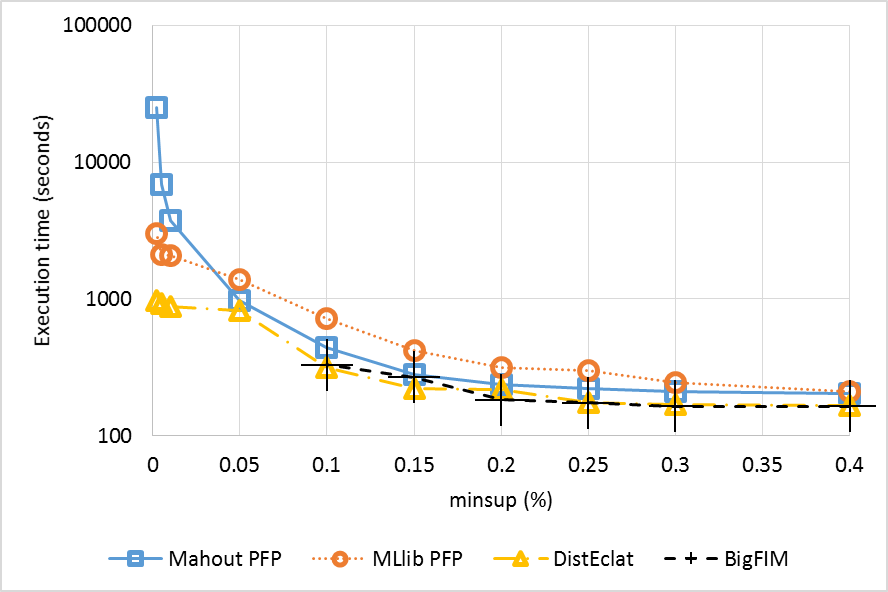
\includegraphics[width=5in]{chapters/survey/immagini/minsup_1_log.png}
\caption{Execution time for different $minsup$ values
(Dataset~\#1), average transaction length~10.}
\label{minsup_1}
\end{figure}


%\begin{figure}[!t]
%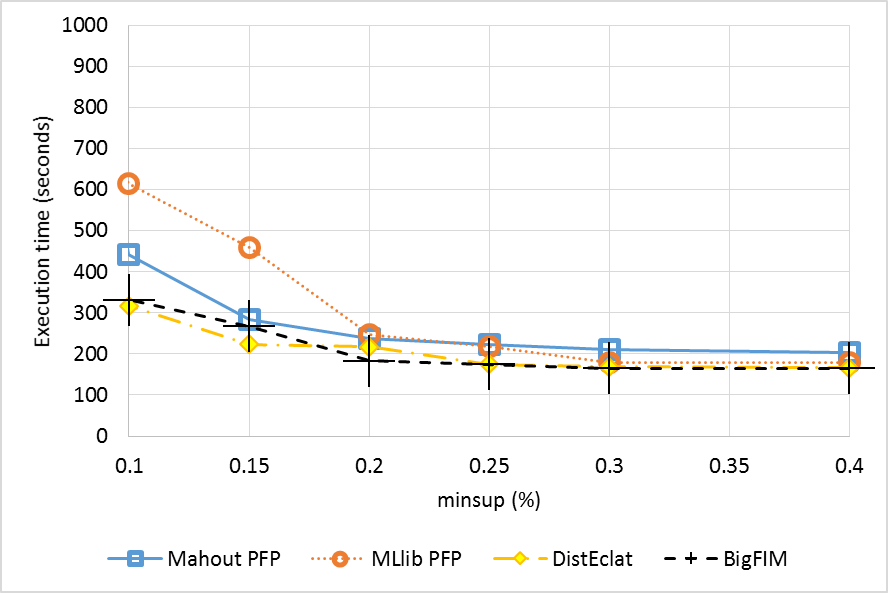
\includegraphics[width=5in]{chapters/survey/immagini/minsup_2.png}
%\caption{Detail of the chart in Figure~\ref{minsup_1} for high $minsup$ values (Dataset~\#1).
%[@FABIO3: da rimuovere, figura precedente ha scala logaritmica.]}
%\label{minsup_2}
%\end{figure}


\begin{figure}[!t]
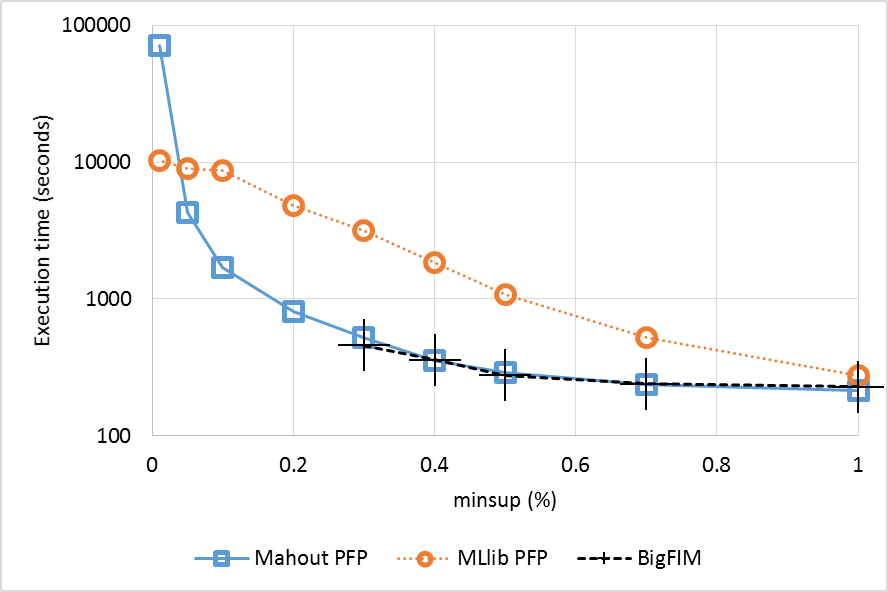
\includegraphics[width=5in]{chapters/survey/immagini/minsup_3_log.png}
\caption{Execution time for different $minsup$ values
(Dataset~\#3), average transaction length~30.}
\label{minsup_3}
\end{figure}



To avoid the bias due to a specific data distribution,
experiments have been executed on two different datasets:
Dataset~\#1 and Dataset~\#3.
They both share the same average length of maximal patterns (5),
the number of different items (100 thousands),
the correlation grade among patterns (0.25), and
the number of transactions (10 millions).
The difference is in the average transaction length:
10 items for Dataset~\#1 and 30 items for Dataset~\#3
(see Table~\ref{datasets_transactions}).
Being constant the rest of the characteristics,
longer transactions lead to a higher dataset density,
which results into a larger number of frequent itemsets.
Furthermore, we can test the performance degradation
when dealing with datasets with a highest number of dimensions.



Figure~\ref{minsup_1} reports the execution time of the itemset mining
algorithms when varying the $minsup$ threshold from 0.002\% to 0.4\% and
considering Dataset~\#1. DistEclat is the fastest algorithm for all the
considered $minsup$ values. However, the improvement with respect to the
other algorithms depends on the value of $minsup$.
When $minsup$ is greater than or equal to 0.2\%, all the implementations show
similar performance, with BigFIM and DistEclat being slightly faster than
Mahout PFP and MLlib PFP.
The performance gap largely increases
with $minsup$ values lower than 0.05\%:
Mahout PFP becomes orders of magnitude slower than both
DistEclat and MLlib PFP.
BigFIM is as fast as DistEclat when $minsup$ is higher than 0.1\%, but below
this threshold BigFIM runs out of memory during the
$k$-Frequent Itemset generation phase, specifically when generating 2-FIs.
MLlib PFP is generally slower than Mahout PFP,
becoming faster only for $minsup$ values below 0.05\%.
Based on this first set of experiments, DistEclat seems to be the
most appropriate choice, with excellent results when very low values of $minsup$ are considered,
followed by MLlib PFP, which can reach very low $minsup$ values with
good performance, at the expense of slightly slower performance for higher $minsup$ values.

% %In this set of experiments, different values of minimum support threshold are
% used to extract the frequent itemsets. The input datasets used are two, with two
% different transaction length: dataset \#1 with 10 items and 10 million
% transactions and dataset \#7, with 30 items and 10 million transactions
% (~\ref{datasets_transactions}).
% %With dataset \#1 and a support above 0,1 \%, all the implementations show
% similar perfomances, as shown in Figure~\ref{minsup_2}, which is an enlargement
% of the the graph in Figure~\ref{minsup_1}. Precisely, BigFIM and DistEclat prove
% to be the fastest implementations. Below this treshold, BigFIM runs out of
% memory, while Mahout PFP completes all the tasks with an execution time much
% higher than the MLlib implementation (almost 6 times).
% % %DistEclat, finally, has the best performance, completing the task with the
% % minimum wallclock time, closely followed by MLlib PFP.
% % %The experiment demostrates that DistEclat and MLlib PFP are the most reliable
% % algorithms when the minsup values start to be very low.

In the second set of experiments, we analyze the execution time of
the algorithms for different minimum support values on Dataset~\#3,
which is characterised by a higher average transaction length
(3 times longer than Dataset~\#1),
and a larger data size on disk (4 times bigger),
with the same number of transactions (10 millions).
Since the mining task is more computationally intensive,
$minsup$ values lower than 0.01\% were
not considered in this set of experiments,
as this has proven to be a limit for most algorithms
due to memory exhaustion or too long experimental duration (days).
Results are reported in Figure~\ref{minsup_3}:
DistEclat runs immediately out of memory
because of the size of the input dataset,
which is transposed in a vertical format during the first phase:
the longer transactions prevent it from completing such step.
MLlib PFP is much slower than Mahout PFP for most $minsup$ values (0.7\% and below),
and BigFIM, as in the previous experiment,
achieves top-level performance, but cannot scale to low $minsup$ values
(the lowest is 0.3\%),
due to memory constraints during the $k$-FI generation phase.
Mahout PFP and MLlib PFP are the only algorithms
to complete the mining tasks for all $minsup$ values.
Precisely,
Mahout PFP is the most suitable technique
when dealing with minsup values over 0.05\%,
with a perfomance 6 to 8 times faster than the MLlib sibling.
However, with lower $minsup$ values,
Spark MLlib becomes the fastest approach with an order of magnitude gap.
We identified the cause of the different performance
between the two PFP implementations
in the different pruning strategies.
The algorithms which extract closed itemsets, such as Mahout PFP,
can apply more effective pruning techniques
that are not applicable when all frequent itemsets must be extracted,
which is the case for MLlib PFP.
%their different mining phases: even if both of them extracts the same set of itemset in this specific use cases, the extraction process is different because MLlib PFP extracts all the frequent itemsets. Mahout PFP, instead, extracts only the closed ones\footnote{The differences are not reported in the paper.}.
%the Spark implementation extracts all the frequent itemsets and then selects the closed ones,
%while the Hadoop implementation directly extracts only the closed frequent itemsets.


Overall,
DistEclat is the fastest approach when it does not run out of memory.
Mahout PFP is the most reliable implementation across almost all $minsup$ values,
even if it is not always the fastest,
sometimes with large gaps behind the top performers.
MLlib is a reasonable tradeoff choice,
as it is constantly able to complete all the tasks in a reasonable time.
%the 2nd fastest approach
%and it is able to reach the 1st or 2nd lowest $minsup$ values.
Finally, BigFIM does not present advantages over the other approaches,
being unable to reach low $minsup$ values and to provide fast executions.

% %Indeed, we can say that DistEclat and MLLib are the best approaches for
% different $minsup$ values analyses but are strongly affected, respectively, by
% dataset size and transaction length. When one of these features increases,
% Mahout PFP is the only algorithm able to complete the tasks.

%\begin{table*}[h!]
%\begin{center}
%\caption{Synthetic datasets used for different transaction length experiments}
%\label{datasets_attributes}
%\begin{tabular}{|c|c|c|c|c|}
%\hline
%{\bf ID }& {\bf IBM Generator} &  {\bf \# different } & {\bf  \# items  } & {\bf size} \\
%{\bf  }& {\bf  parameters } &  {\bf items  } & {\bf per } & {\bf (GB) } \\
%{\bf  } & {\bf } & {\bf } & {\bf  transaction } & {\bf } \\ \hline
% \hline
%6  & T20P5I100kC0.25D10000k  & 18011 & 29.99 & 1187 \\ \hline
%7  & T30P5I100kC0.25D10000k  & 18011 & 29.99 & 1776 \\ \hline
%8 & T40P5I100kC0.25D10000k  & 18010 & 39.98 & 2364 \\ \hline
%9 & T50P5I100kC0.25D10000k  & 18014 & 49.98 & 2953 \\ \hline
%10 & T60P5I100kC0.25D10000k  & 18010 & 59.98 & 3541 \\ \hline
%11 & T70P5I100kC0.25D10000k  & 18016 & 69.98 & 4130 \\ \hline
%12 & T80P5I100kC0.25D10000k  & 18012 & 79.98 & 4719 \\ \hline
%13 & T90P5I100kC0.25D10000k  & 18014 & 89.97 & 5307 \\ \hline
%14 & T100P5I100kC0.25D10000k & 18015 & 99.97 & 5896 \\ \hline
%\end{tabular}
%\end{center}
%\end{table*}



%\begin{table*}[h!]
%\begin{center}
%\caption{Synthetic datasets used for different pattern lengths}
%\label{datasets_patterns1}
%\begin{tabular}{|c|c|c|c|c|c|}
%\hline


%{\bf ID }& {\bf IBM Generator parameters } & {\bf Number of } & {\bf Average number of } & {\bf size} \\
%{\bf  } & {\bf } & {\bf different items } & {\bf items per transaction } & {\bf } \\ \hline
% \hline
%15 & T20P2I100kC0.25D10000k  & 8212 & 19,99 & 1.188 \\ \hline
%16 & T20P4I100kC0.25D10000k & 14976 & 19,99 & 1.187 \\ \hline
%17 & T20P6I100kC0.25D10000k  & 20727 & 19,99 &1.187 \\ \hline
%18 & T20P8I100kC0.25D10000k & 25864 & 20,03 &1.188 \\ \hline
%19 & T20P10I100kC0.25D10000k & 30215 & 20,09 &1.192 \\ \hline
%20 & T20P12I100kC0.25D10000k &  34233 & 20,26 &1.202 \\ \hline
%21 & T20P14I100kC0.25D10000k &  37672 & 20,56 & 1.221 \\ \hline
%22 & T20P16I100kC0.25D10000k &  40955 & 21,04 & 1.249 \\ \hline
%
%\end{tabular}
%\end{center}
%\end{table*}






%\begin{table*}[]
%\begin{center}
%\caption{Synthetic datasets used for different pattern lengths}
%\label{datasets_patterns2}
%\begin{tabular}{|c|c|c|c|c|c|}
%\hline
%{\bf ID }& {\bf IBM Generator parameters } & {\bf Number of transactions } & {\bf Number of } & {\bf Average number of } & {\bf size} \\
%{\bf  }& {\bf } & {\bf } & {\bf different items } & {\bf items per transaction } & {\bf } \\ \hline
% \hline
%22 & T40P2I100kC0.25D10000k & 10.000.000 & 8215 & 39,99 & 2,4 GB \\ \hline
%23 & T40P4I100kC0.25D10000k & 10.000.000 & 14,979 & 39,99 & 2,4 GB \\ \hline
%24 & T40P6I100kC0.25D10000k & 10.000.000 & 20733 & 39,98 & 2,4 GB \\ \hline
%25 & T40P8I100kC0.25D10000k & 10.000.000 & 25864 & 39,98 & 2,4 GB \\ \hline
%26 & T40P10I100kC0.25D10000k & 10.000.000 & 30220 & 39,99 & 2,4 GB \\ \hline
%27 & T40P12I100kC0.25D10000k & 10.000.000 & 34262 & 39,98 & 2,4 GB \\ \hline
%28 & T40P14I100kC0.25D10000k & 10.000.000 & 37673 & 39,98 & 2,4 GB \\ \hline
%29 & T40P16I100kC0.25D10000k & 10.000.000 & 40971 & 39,98 & 2,4 GB \\ \hline
%\end{tabular}
%\end{center}
%\end{table*}


%%
%%\begin{table*}[h!]
%%\begin{center}
%%\caption{Experimental result summary for $minsup$ impact, Section~\ref{minsup_exp}}
%%\label{minsup_resume}
%%\begin{tabular}{|c|c|c|c|c|}
%%\hline
%%\textbf{}          & \multicolumn{2}{l|}{\textbf{Transaction length: 10}} & \multicolumn{2}{l|}{\textbf{Transaction length: 30}} \\ \hline
%%\textbf{algorithm} & \textbf{lowest $minsup$}        & \textbf{speed}        & \textbf{lowest $minsup$}        & \textbf{speed}        \\ \hline
%%Mahout PFP         & 0.002 \%                       & 3rd                  & 0.01 \%                         & 2nd                 \\ \hline
%%MLlib PFP          & 0.002 \%                       & 2nd                  & 0.01 \%                         & 1st                  \\ \hline
%%BigFIM             & 0.1 \%                         & 4th        	   & 0.3 \%                         & 3rd                  \\ \hline
%%DistEclat          & 0.002 \%                       & 1st                  & -                              & -                    \\ \hline
%%\end{tabular}
%%\end{center}
%%\end{table*}
%%




\subsection{Impact of the average transaction length}
\label{attributes_exp}

This section compares the execution times of the selected approaches
on datasets with different average transaction lengths,
from 10 to 100 items per transaction,
and fixed values of 10 million transactions, and 1\% $minsup$.
To this aim, Datasets \#1--10 were used (see Table~\ref{datasets_transactions}).
Longer transactions often lead to more dense datasets and a larger number of longer frequent itemsets.
This generally corresponds to more computationally intensive tasks.
The execution times obtained are reported in Figure~\ref{attributes}.
BigFIM and DistEclat execution times for transaction length of 10 and 20 are not reported because, for these configurations, not enough 3-itemsets are extracted.
For higher transaction lengths, DistEclat is not included since it runs out of memory
for values beyond 20 items per transaction.
The other algorithms have similar execution times for short transactions,
up to 30 items.
For longer transactions, a clear trend is shown:
(i) MLlib PFP is much slower than the others
and it is not able to scale for longer transactions,
as its execution times abruptly increase until it runs out of memory
beyond 60 items per transaction;
(ii) Mahout PFP and BigFIM have a similar trend until 70 items per transactions,
when Mahout PFP becomes slower than BigFIM.
Despite the Apriori-based initial phase,
BigFIM proved to be the best scaling approach for very long transactions.
The FP-growth based approaches, instead,
are affected by the increasing length of the transactions.
%Despite the Apriori-based initial phase, BigFIM shows to be the mo
%PFP is not optmized to address long transactions due to its FP-tree structure,
%whereas BigFIM is able to address denser data distributions and a large
%number of attributes.


%\begin{table*}[h!]
%\begin{center}
%\caption{Experimental result summary for transaction length impact, Section~\ref{attributes_exp}}
%\label{transaction_length_resume}
%\begin{tabular}{|c|c|c|}
%\hline
%
%\textbf{algorithm} & \textbf{reached transaction length}        & \textbf{speed}        \\ \hline
%BigFIM             & 100                        & 1st        	                  \\ \hline
%Mahout PFP         & 100                       & 2nd                          \\ \hline
%MLlib PFP          & 60                       & 3rd                                 \\ \hline
%DistEclat          & -                       & -                            \\ \hline
%\end{tabular}
%\end{center}
%\end{table*}
%


% % COMMENTO A FIGURA 5 RIMOSSA
% In order to assess this type of experiments with the ones of the Section
% \ref{minsup_exp}, we have performed a set of experiments dealing with datasets
% of both a varying transaction length (focusing on datasets with an average
% number of items from 10 to 30) and different minsup values (0.01\% and 0.05\%).
% % %We also performed a set of experiments with the same datasets lowering the
% % minimum support threshold (we considered $minsup$=0.01\% and $minsup$=0.05\%) .
% The results are reported in Figure \ref{attributes_2}.  The execution time of
% BigFIM is not reported because, as already evidenced in Section
% \ref{minsup_exp},  it is unable to complete the mining task when
% low values of minsup are considered. On the other hand, different performances
% of Mahout PFP and MLlib PFP are noticeable. When the $minsup$ is 0.05\% Mahout
% PFP is
% still faster than MLlib PFP. Indeed, when the $minsup$ value is 0.01\% MLlib
% becomes faster
% than Mahout PFP. Hence, this results confirm that MLlib is the best approach
% when dealing with very low $minsup$ values.




% %The difference between the performance of Mahout PFP and MLlib PFP, as before,
% may be caused by the difference mining processes. Since Mahout PFP
% %mines only the frequent closed itemsets, it can exploit more effective pruning
% techniques and reduce the depth of the recursive mining phase. Differently,
% %MLlib PFP, which mines all the frequent itemsets, has a deeper recursive mining
% phase, in particular when long transactions are considered.
% %The difference between the performance of Mahout PFP and MLlib PFP, as before,
% may be caused by the difference mining processes which lead to different type
% %of outputs, even if, in this specific case, the number of frequent itemsets
% matches the number of closed ones.

\begin{figure}[!t]
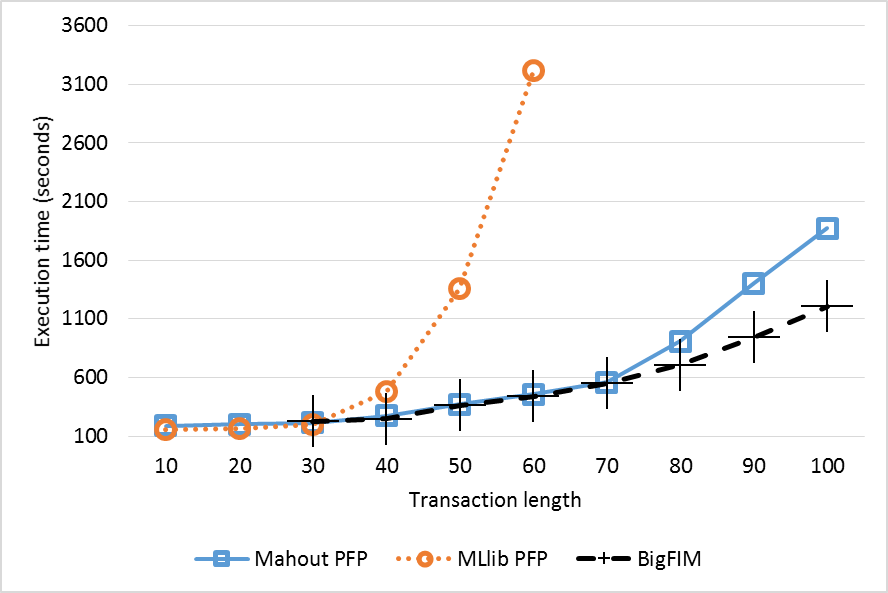
\includegraphics[width=5in]{chapters/survey/immagini/attributes.png}
\caption{Execution time with different average transaction lengths
(Datasets \#1--10, $minsup$ 1\%).}
\label{attributes}
\end{figure}

% \begin{figure}[!t]
% 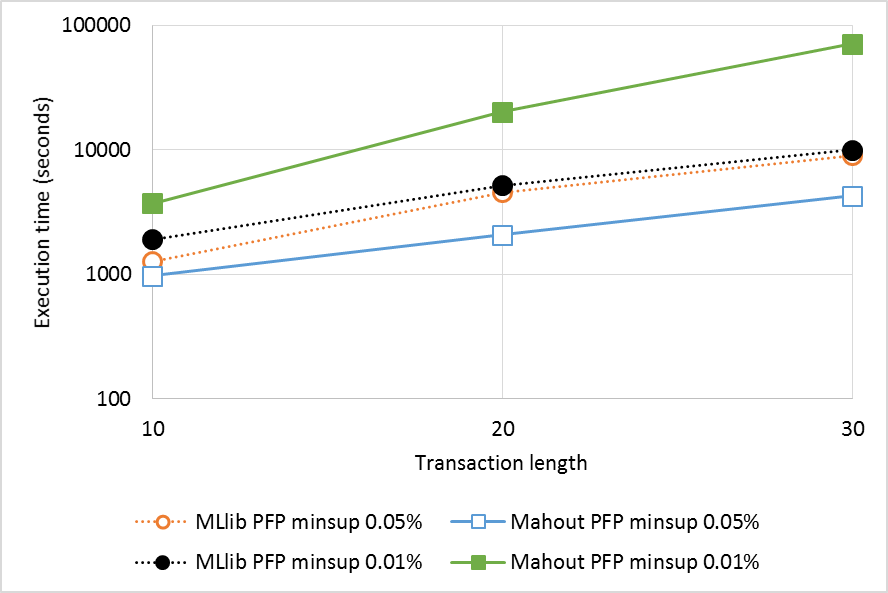
\includegraphics[width=5in]{chapters/survey/immagini/attributes_2.png}
% \caption{Execution time with different average transaction lengths,
% and $minsup$ values 0.01\% and 0.05\%.}
% \label{attributes_2}
% \end{figure}



% %ELIMINARE DA QUI
% %The second set of experiments studies the performance of the approaches dealing
% with datasets obtained setting different expected frequent patterns length. We
% utilised a configuration with 20 attributes and another with 40 (respectively
% detailed in tables ~\ref{datasets_patterns1} and ~\ref{datasets_patterns2}) with
% different expected patterns length. Therefore, the datasets of these evaluation
% differ for their density. A higher expected pattern length is typical of dense
% dataset distributions, while sparse datasets are characterised by many short
% itemsets.
% %The minsup value is set to 0,25\% for the first set of experiments and to
% 0,40\% for the second one. We changed the minsup values in order to have
% significative output and a good number of approaches that not run out of memory.
% %
% %In the first case, DistEclat was able to run even if it showed memory issues
% for the longest expected patterns, as illustrated in the graph in
% Figure~\ref{pattern_small}. Even in this experiment, BigFIM performances
% revealed to be the most stable of the set of algorithms for all the pattern
% length configurations, even if Mahout PFP is not far. MLlib implementation is
% able to execute all the tasks, but it shows a serious gap when the expected
% patterns are short. This is very interesting, because one can expect a behaviour
% more similar to the one of the previous experiment, where the execution time
% strongly increases together with the average transaction length of the input
% dataset. Clearly, the perforamance related to the average length of transactions
% and the average length of the expected patterns are not correlated.
% %We counted the frequent itemsets produced to understand if the performance
% degradation was reasoned by an explosion of the number of itemsets. As repored
% in Table~\ref{extracted_itemsets}, this was not the case.
% %
% %In the second case, with an average transaction length of 40 items and a minsup
% of 0,4\%, the behaviour of the algorithms is very similar, except for DistEclat
% that is not able to mine the input. BigFIM shows the best performance followed
% by Mahout PFP, which has apeak corresponding to an expected pattern length of
% 14. The behaviour is similar to the previous experiment, in which it was less
% explicit. In these cases, the number of extracted itemset is much higher than
% the previous case, as shown in Table~\ref{extracted_itemsets}. Above all, the
% high execution time is caused by a not proper load balancing. In fact, almost
% all the tasks of the mining MapReduce job of the process finish the computation
% below a minute of wall clock time, one of them reaches 3 minutes while the last
% 2 last respectively take over 8 minutes and over 32 minutes. This validates the
% assumption about Mahout PFP load balancing in subSection ~\ref{FP-Growth}.
%




%\begin{table*}[h!]
%\begin{center}
%\caption{Synthetic datasets used for different pattern lengths}
%\label{datasets}
%\begin{tabular}{|c|c|c|c|c|c|}
%\hline
%
%ID & IBM Generator  & Number of  & Number of  & Average number & size\\
% & parameters & transactions & different & of items per & \\
% & &  &  items & transaction &\\ \hline
%14 & T20P2I100kC0.25D10000k & 10.000.000 & 8212 & 19,99 & 1,2 GB \\ \hline
%15 & T20P4I100kC0.25D10000k & 10.000.000 & 14976 & 19,99 & 1,2 GB \\ \hline
%16 & T20P6I100kC0.25D10000k & 10.000.000 & 20727 & 19,99 & 1,2 GB \\ \hline
%17 & T20P8I100kC0.25D10000k & 10.000.000 & 25864 & 20,03 & 1,2 GB \\ \hline
%18 & T20P10I100kC0.25D10000k & 10.000.000 & 30215 & 20,09 & 1,2 GB \\ \hline
%19 & T20P12I100kC0.25D10000k & 10.000.000 & 34233 & 20,26 & 1,2 GB \\ \hline
%20 & T20P14I100kC0.25D10000k & 10.000.000 & 37672 & 20,56 & 1,2 GB \\ \hline
%21 & T20P16I100kC0.25D10000k & 10.000.000 & 40955 & 21,04 & 1,2 GB \\ \hline
%
%\end{tabular}
%\end{center}
%\end{table*}
%
%\begin{table*}[h!]
%\begin{center}
%\caption{Synthetic datasets used for different pattern lengths}
%\label{datasets}
%\begin{tabular}{|c|c|c|c|c|c|}
%\hline
%
%ID & IBM Generator  & Number of  & Number of  & Average number & size\\
% & parameters & transactions & different & of items per & \\
% & &  &  items & transaction &\\ \hline
%22 & T40P2I100kC0.25D10000k & 10.000.000 & 8215 & 39,99 & 2,4 GB \\ \hline
%23 & T40P4I100kC0.25D10000k & 10.000.000 & 14,979 & 39,99 & 2,4 GB \\ \hline
%24 & T40P6I100kC0.25D10000k & 10.000.000 & 20733 & 39,98 & 2,4 GB \\ \hline
%25 & T40P8I100kC0.25D10000k & 10.000.000 & 25864 & 39,98 & 2,4 GB \\ \hline
%26 & T40P10I100kC0.25D10000k & 10.000.000 & 30220 & 39,99 & 2,4 GB \\ \hline
%27 & T40P12I100kC0.25D10000k & 10.000.000 & 34262 & 39,98 & 2,4 GB \\ \hline
%28 & T40P14I100kC0.25D10000k & 10.000.000 & 37673 & 39,98 & 2,4 GB \\ \hline
%29 & T40P16I100kC0.25D10000k & 10.000.000 & 40971 & 39,98 & 2,4 GB \\ \hline
%\end{tabular}
%\end{center}
%\end{table*}




\subsection{Impact of the number of transactions}
\label{transaction_exp}

\begin{figure}[!t]
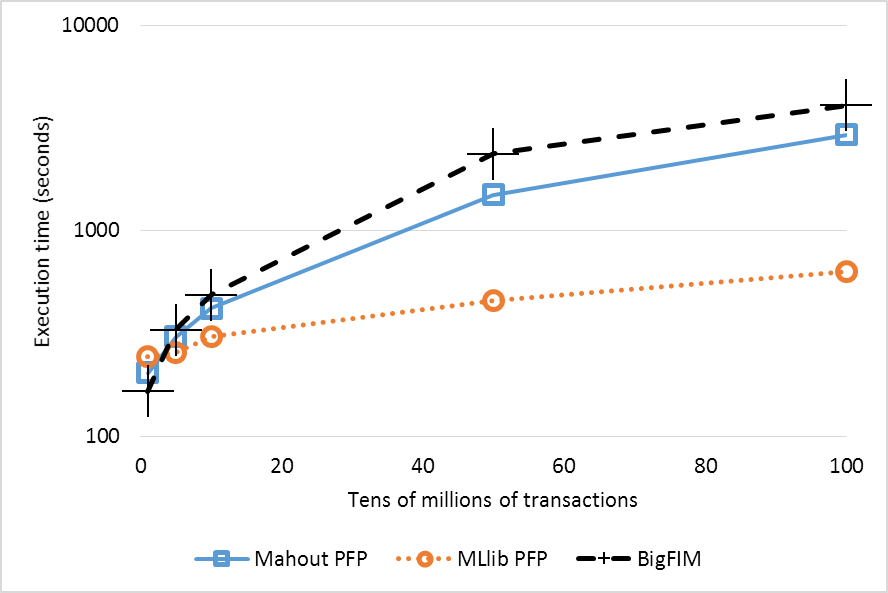
\includegraphics[width=5in]{chapters/survey/immagini/transactions_log.png}
\caption{Execution time with different numbers of transactions
 (Datasets \#1, \#11--14,
 $minsup$~0.4\%,
 average transaction length~10).}
\label{transactions}
\end{figure}

This section evaluates the effect of varying the number of transactions,
i.e., increasing the dataset size without changing intrinsic data characteristics,
such as the transaction length or the data distribution.
To this aim, Datasets \#1, \#11--14 have been used
(see Table~\ref{datasets_transactions}),
which have a number of transactions
ranging from 10 millions to 1 billion.
The average transaction length is fixed to 10, and the $minsup$ is 0.4\%,
which is the highest value for which the mining leverages both the two phases of
BigFIM and DistEclat, and it corresponds to the highest value used
in the experiments of Section~\ref{minsup_exp}.

As shown in Figure~\ref{transactions}, all the considered algorithms scale
linearly with respect to the dataset cardinality, with BigFIM being the slowest,
closely followed by Mahout PFP,
and with MLlib PFP being by far the fastest approach,
with execution times reduced by almost an order of magnitude.
BigFIM is paying the iterative disk reading activities
during its initial Apriori phase.
PFP implementations, instead, read from the disk only twice.
Finally, DistEclat fails under its assumption that the entire dataset should
be stored in each node, and it is not able to complete the extraction beyond
10 million transactions.

%\begin{table*}[h!]
%\begin{center}
%\caption{Experimental result summary for number of transactions impact, Section~\ref{transaction_exp}}
%\label{transaction_resume}
%\begin{tabular}{|c|c|c|}
%\hline
%
%\textbf{algorithm} & \textbf{reached dataset size}        & \textbf{speed}      \\
%\textbf{algorithm} & \textbf{tens of millions of transactions}        &      \\ \hline
%MLlib PFP          & 100                       & 1st                               \\ \hline
%Mahout PFP         & 100                       & 2nd                          \\ \hline
%BigFIM             & 100                        & 3rd       	                  \\ \hline
%DistEclat          & 1                       &  -                            \\ \hline
%\end{tabular}
%\end{center}
%\end{table*}







\subsection{Real use cases}
\label{usecases}

In the following, we analyze the performance of the mining algorithms in two
real-life scenarios:
(i) URL tagging of the Delicious dataset and
(ii) network traffic flow analysis.
The characteristics of the two datasets
are reported in Table~\ref{datasets_real}.

\begin{table*}[h!]
\scriptsize
\begin{center}
\caption{Real-life use-cases dataset characteristics}
\label{datasets_real}
\begin{tabular}{|c|c|c|c|c|c|}
\hline
{\bf ID }& {\bf Name} 	&  {\bf Num. of} 	& {\bf  Avg. \# items} 			& {\bf Size} \\
{\bf  }& {\bf  } 		&  {\bf different items} 	& {\bf  per transaction} 	& {\bf (GB) } \\
\hline
\hline
15& Delicious & 57,372,977 & 4 & 44.5 \\ \hline
16 & Netlogs & 160,941,600 & 15 & 0.61  \\ \hline
\end{tabular}
\end{center}
\end{table*}





\subsubsection{URL tagging}
\label{delicious_exp}

In this experiment, we evaluate the selected algorithms in a real-life use case
by using the Delicious dataset~\cite{wetzker2008analyzing}, which is a
collection of web tags.
Each record represents the tag assigned by a user to a URL and it consists of
4 attributes:
date,
user id (anonymized),
tagged URL,
and tag value.
The transactional representation of the Delicious dataset includes
one transaction for each record, where each transaction is a set of four pairs
(attribute, value), i.e., one pair for each attribute.
The dataset stores more than 3 years of web tags.
The dataset is very sparse because it has a huge number of different URLs
and tags.
Additional characteristics of the dataset are reported
in Table~\ref{delicious_itemsets}.

This experiment simulates the environment of a service provider that
periodically analyses the web tag data to extract frequent patterns: they
represent the most frequent correlations among tags, URLs, users, and dates.
Many different use cases can fit this description:
tag prediction, topic classification, trend evolution, etc.
Their evolution over time is also interesting.
To this aim, the frequent itemset extraction has been executed
cumulatively on temporally adjacent subsets of data,
whose length is a quarter of year (i.e., first quarter,
then first and second quarter, then first, second, and third quarter, and so on,
as if the data were being colleted quarterly and analyzed as a whole at the
end of each quarter).
The setting of $minsup$ in a realistic use-case proved to be a critical choice.
Too low values lead to millions of itemsets,
which become useless as they exceed the human capacity to understand the results.
However, too high $minsup$ values would discard longer itemsets,
which are more meaningful
as they better highlight more complex correlations
among the different attributes and values.
Furthermore, we wanted to obtain at least 3-itemsets to assess
the BigFIM two phases, without reducing it to a pure DistEclat.
As a result of these constraints and of the high sparsity of the dataset,
we identified the setting $minsup$=0.01\% as the best tradeoff.

\begin{table}[h]
\scriptsize
\begin{center}
\caption{Delicious dataset: cumulative number of transactions and frequent itemsets
with $minsup$~0.01\%.}
\label{delicious_itemsets}
\begin{tabular}{|c|c|c|c|}
\hline
{\bf Up to year,}	& {\bf Number of} 	& {\bf	Number of} \\
{\bf month, quarter}	& {\bf transactions} 	& {\bf	frequent itemsets} \\
\hline \hline
2003 Dec, Q4 	& 153,375	 	& 7197 \\ \hline
2004 Mar, Q1  	& 489,556		& 6013 \\ \hline
2004 Jun, Q2	& 977,515		& 5268 \\ \hline
2004 Sep, Q3 	& 2,021,261		& 5084 \\ \hline
2004 Dec, Q4 	& 4,349,209		& 4714 \\ \hline
2005 Mar, Q1	& 9,110,195		& 4099 \\ \hline
2005 Jun, Q2	& 15,388,516		& 3766 \\ \hline
2005 Sep, Q3	& 24,974,689		& 3402 \\ \hline
2005 Dec, Q4	& 41,949,956		& 3090 \\ \hline
\end{tabular}
\end{center}
\end{table}

\begin{figure}[!t]
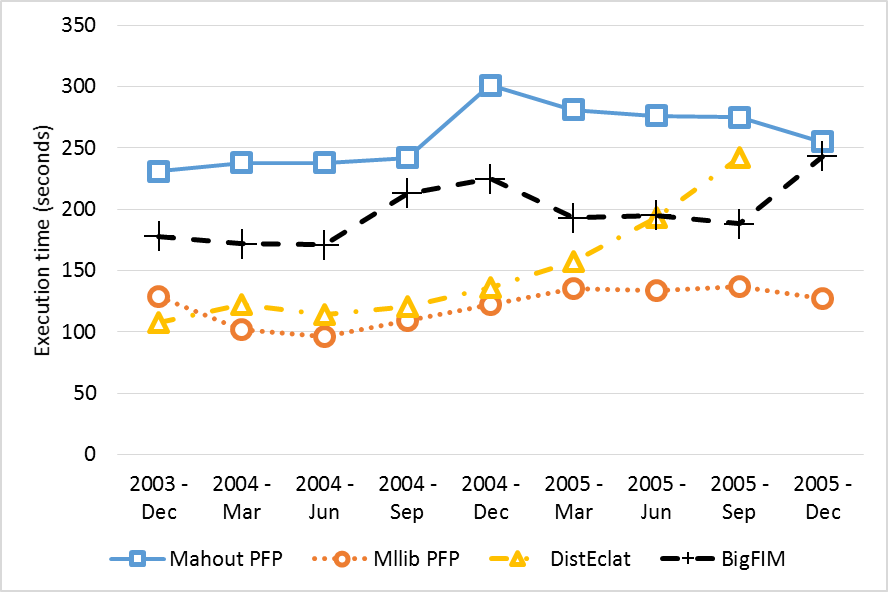
\includegraphics[width=5in]{chapters/survey/immagini/delicious.png}
\caption{Execution time for different periods of time on the Delicious dataset
($minsup$=0.01\%)}
\label{delicious}
\end{figure}


Table~\ref{delicious_itemsets} reports the cumulative number of
transactions for the different periods of time
(i.e., the cardinality of the input dataset) and the
number of frequent itemsets extracted with a fixed $minsup$ of 0.01\%,
while the execution times of the
different algorithms are shown in Figure~\ref{delicious}.


MLlib consistently proves to be the fastest approach, with DistEclat following.
However, while DistEclat is slightly faster than MLlib only with the first, smallest dataset
(up to Dec 2003, with 150 thousands transactions), when the dataset size increases,
DistEclat execution times do not scale, and it eventually fails for the final
40-million-transaction dataset of Dec 2005, due to memory exhaustion.
BigFIM and Mahout PFP consistently provide 2 to 3 times longer execution times.
Apart from DistEclat, all algorithms complete the task with similar performance
despite increasing the dataset cardinality from 150 thousand transactions to 41 millions,
thanks to the constant relative $minsup$ threshold
which reduces the number of frequent itemsets
for decreasing density of the dataset.
To sum up, MLlib is the best choice for short transactions
(this dataset length is 4),
independently of the dataset cardinality and density.


% %Therefore, we extracted the frequent itemset related to an incremental period
% of time covering 4 years of tags.
% %For this scope, we were forced to change the minsup values in some experiments.
% The choice of the minsup value strongly impacts the results. On one hand we did
% not want to want to extract a billion of itemsets, because they would not be
% realistically processable. On the other hand, we did not want just a list of
% items (header table) which can be obtained with the most trivial Word Count
% MapReduce implementation. Furthermore, we wanted to obtain at least some
% 3-itemsets in order to exploit the BigFIM two phases, without reducing it to a
% pure DistEclat.
% %
% %The choice was made harder by the dataset sparsity. Adding a new period of time
% to the computation corresponds to new transactions in the input datasets.
% However, adding new transactions means adding new items of such a sparse
% dataset. In few words, the sparsity of the input dataset grows up faster than
% the number of transactions. Consequently, the same minimum support thresholds
% for each scrape of dataset would not always carry to the desired ouput. It would
% lead to a very intensive task and a very high number of frequent itemsets when
% the transactions are few; it would not result low or deep enough to extract a
% significative number of itemset when the number of transactions is high, because
% of the sparsity of the dataset. For this reason, we deepened the minsup value
% for the computation related to the transaction related to the last year of tags,
% as shown in Table~\ref{delicious_itemsets}.
% %The execution time of the different algorithms are shown in the graph in
% Figure~\ref{delicious}. DistEclat revealed to be the most performant approach
% before running out of memory. This is something unexpected because the
% depth-first search strategy hardly fits sparse dataset distributions. BigFIM
% outperforms Mahout PFP while MLlib implementation revealed to be the most
% reliable solution, with an almost flat curve.



%\begin{table}[h]
%\begin{center}
%\caption{Number of tags for year and minsup used for Delicious}
%\label{delicious_itemsets}
%\begin{tabular}{|c|c|c|c|}
%\hline
%{\bf Year }	& {\bf Tags} & {\bf minsup (\%) } & {\bf	frequent itemsets } \\ \hline \hline
%2003	& 153375	 & 0.01 &	7197 \\ \hline
%2004 &	4195834	& 0.01	& 4714 \\ \hline
%2005	& 37600747	& 0.01	& 3090 \\ \hline
%2006	& 130799274	& 0.005 &	5321 \\ \hline
%\end{tabular}
%\end{center}
%\end{table}





\subsubsection{Network traffic flows}
\label{net_exp}


\begin{figure}[!t]
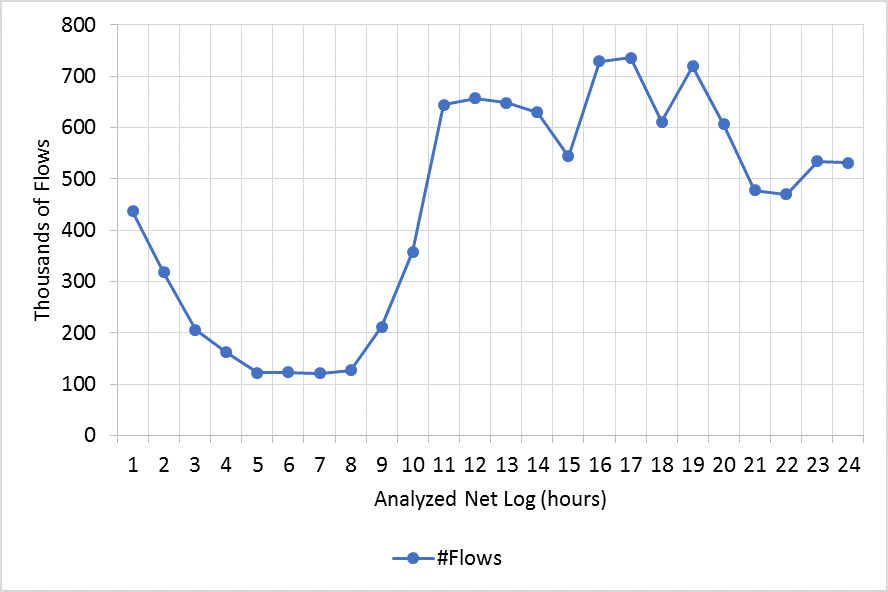
\includegraphics[width=5in]{chapters/survey/immagini/number_flows.png}
\caption{Number of flows for each hour of the day.}
\label{number_flows}
\end{figure}

\begin{figure}[!t]
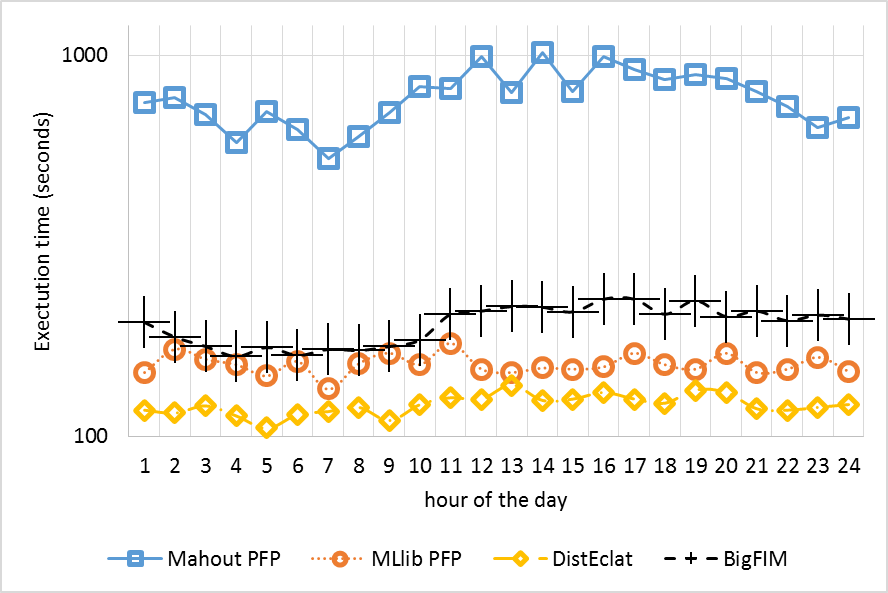
\includegraphics[width=5in]{chapters/survey/immagini/net_logs_log.png}
\caption{Execution time of different hours of the day.
(dataset 31, $minsup$=1\%)}
\label{net}
\end{figure}


\begin{table}[h!]
\scriptsize
\begin{center}
\caption{Network traffic flows: number of transactions and frequent itemsets
with $minsup$~0.1\%.}
\label{netlog_itemsets}
\begin{tabular}{|c|c|c|}
\hline
{\bf Hour of}	& {\bf Number of} 	& {\bf	Number of} \\
{\bf the day}	& {\bf transactions} 	& {\bf	frequent itemsets} \\
\hline \hline
0.00  & 437,417 & 166,217 \\ \hline
1.00  & 318,289 & 173,960 \\ \hline
2.00  & 205,930 & 163,266 \\ \hline
3.00  & 162,593 & 166,344 \\ \hline
4.00  & 122,102 & 157,069 \\ \hline
5.00  & 123,683 & 164,493 \\ \hline
6.00  & 121,346 & 170,129 \\ \hline
7.00  & 127,056 & 159,921 \\ \hline
8.00  & 211,641 & 169,751 \\ \hline
9.00  & 357,838 & 187,912 \\ \hline
10.00 & 644,408 & 191,867 \\ \hline
11.00 & 656,965 & 183,021 \\ \hline
12.00 & 648,206 & 184,279 \\ \hline
13.00 & 630,434 & 180,384 \\ \hline
14.00 & 544,572 & 175,252 \\ \hline
15.00 & 729,518 & 192,992 \\ \hline
16.00 & 735,850 & 189,160 \\ \hline
17.00 & 611,582 & 177,808 \\ \hline
18.00 & 719,537 & 179,228 \\ \hline
19.00 & 607,043 & 174,783 \\ \hline
20.00 & 477,760 & 161,153 \\ \hline
21.00 & 470,291 & 159,065 \\ \hline
22.00 & 534,103 & 144,212 \\ \hline
23.00 & 531,276 & 164,516 \\ \hline
\end{tabular}
\end{center}
\end{table}

This use case evaluates the approaches in a network environment by
using a network traffic log dataset, where each transaction represents a TCP flow.
A network flow is a bidirectional communication between a client and a server.
The dataset has been gathered through Tstat~\cite{Tstat,Tstat2}, a popular
internet traffic sniffer broadly used in
literature~\cite{giordano2015youlighter,ApilettiBCCG13},
by performing a one day capture in three different vantage points
of a nation-wide Internet Service Provider in Italy.
Each transaction of the dataset is associated with
a flow and consists of pairs $(flow~feature, value)$. These features can be
categorical (e.g., TCP Port, Window Scale) or numerical (e.g., RTT,
Number of packets, Number of bytes). We applied a proper preprocessing step in
which numerical attributes have been discretized by using the same
approach adopted in~\cite{ApilettiBCCG13}.
Finally, we have divided the set of flows (i.e., the set of transactions)
in 1-hour slots, generating 24 sub-datasets.
The number of flows in each sub-dataset
is reported in Figure~\ref{number_flows}.

In this use case, the network administrator is interested in performing hourly
analysis to shape the hourly network traffic.
Hence, we evaluated the performance of the four algorithms,
comparing their execution time, on the 24 hourly sub-datasets.
For all the 24 experiments $minsup$ was set to 1\%, which was
the tradeoff value allowing all the algorithms to complete the extraction,
leveraging both the mining phases of BigFIM and DistEclat,
and extracting a reasonable number of frequent itemsets
(details in Table~\ref{netlog_itemsets}).

Results are reported in Figure~\ref{net}, where the performance of the
different approaches show a clear trend: DistEclat always achieves the
lowest execution time, followed by MLlib PFP and BigFIM.
Mahout PFP is the slowest.
The execution time is almost independent of the dataset cardinality,
as it slightly changes throughout the day.
The low dataset size (less than 1~Gigabyte overall)
and cardinality (less than 1~million transactions) make this the ideal
use case for DistEclat, which strongly exploits in-memory computation.



\subsection{Load balancing}
\label{load_exp}


\begin{figure*}[!t]
\begin{center}
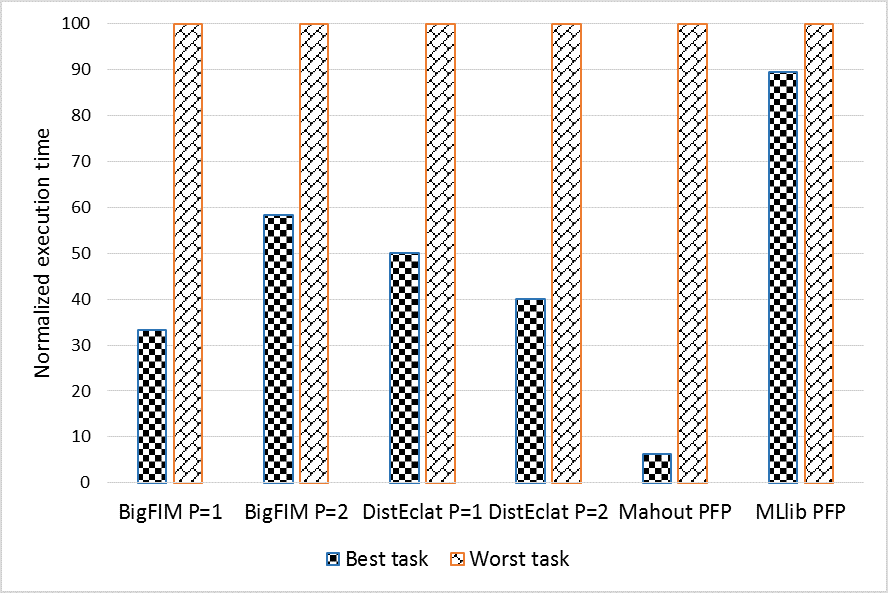
\includegraphics[width=5in]{chapters/survey/immagini/load_balance_big.png}
\caption{Normalized execution time of the most unbalanced tasks.}
\label{load_balance_big}
\end{center}
\end{figure*}

\begin{figure*}[!t]
\begin{center}
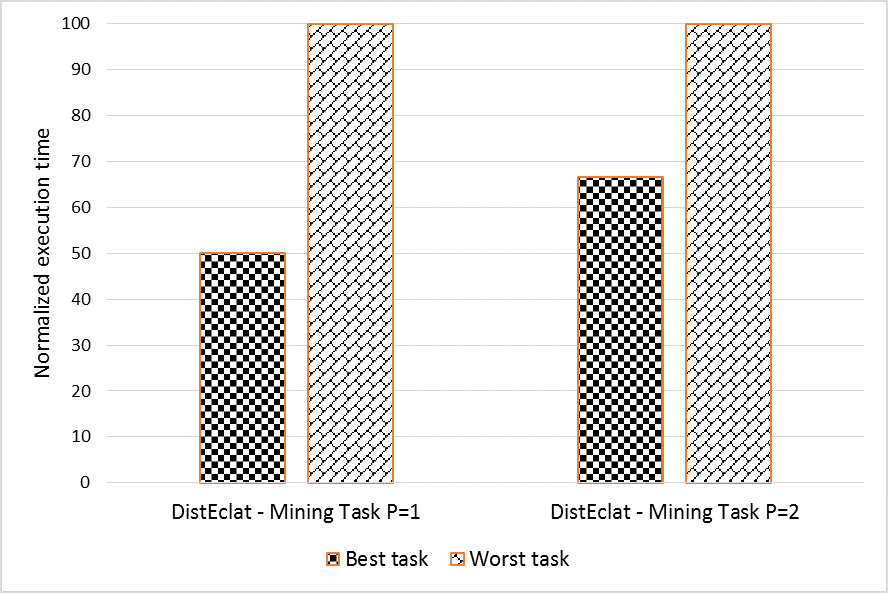
\includegraphics[width=5in]{chapters/survey/immagini/load_balance_disteclat.png}
\caption{Normalized execution time of the most unbalanced tasks of DistEclat.}
\label{load_balance_disteclat}
\end{center}
\end{figure*}

In this section, experiments address the evaluation of the load balancing
strategies of the different approaches, an often underestimated issue
in the distributed data mining bibliography (see Section~\ref{criteria}).
% %The reason is related to the trend to implement in distributed environment
% families of algorithms which were not designed to be distributed.
% %%An example of a bad load balance is what shown in subSection
% ~\ref{attributes_exp} with Mahout PFP: a single task, with an execution period
% more than 30 times higher to the average wallclock time, slows down the whole
% process. On the other hand, approaches such as BigFIM or DistEclat were
% developed taking into account load balance.

Experiments measure the load balancing on a 1-hour-long subset of the
network log dataset (Table~\ref{datasets_real}) with a fixed $minsup$ of 1\%.
We consider the most unbalanced jobs of each algorithm
and compare the execution times of the fastest and the slowest tasks.
To this aim, we are not interested in the absolute execution time,
but rather in the normalized execution times, where the slowest task is
assigned a value of 100, and the fastest task is compared to such value,
as reported in Figure~\ref{load_balance_big}.

MLlib PFP achieves the best load balancing, with comparable
execution times for all tasks throughout all nodes,
whose difference is in the order of 10\%.
Mahout PFP, instead, shows the worst load balancing issues,
with differences as high as 90\%.

We included BigFIM and DistEclat with 2 different
first-phase prefix sizes.
For BigFIM, the experiment confirms that a configuration with longer prefixes
leads to a more balanced mining tasks than a configuration with short-sized prefixes,
as mentioned in Subsection~\ref{bigfim}.
Regarding DistEclat, instead, the behavior is the opposite,
but the values are misleading: considering only the second phase of DistEclat,
where the trees are mined, as shown in Figure~\ref{load_balance_disteclat},
the longer the prefixes, the more balanced the mining tasks.
Hence, DistEclat shows a medium-balanced overall behavior with 1-sized prefixes
(50\% difference between fastest and slowest tasks),
a good load balancing for the second phase with 2-sized prefixes (30\% difference),
and a bad load balancing for the first phase, which affects the overall behavior,
leading to a final 60\% difference, due to the distribution of the prefixes to
the different nodes, their expansion and pruning.
% %
% %(NUOVA PER PAOLO) We have also taken into account an experimental evaluation of
% communication cost, fundamental in such a distributed environment. However, it
% is a very hard evaluation: data about the actual quantity of data is not
% accurate in the resource manager. Even if measuring the ``shuffle read''
% statistics, they don't actually distinguish what was already in the local node
% and what was obtained through the network. Finally, even the data among the
% Spark and the Hadoop distribution are not consistent so they are very hard to
% compare.






\subsection{Communication costs}
\label{communication_costs}

\begin{figure*}[!t]
\begin{center}
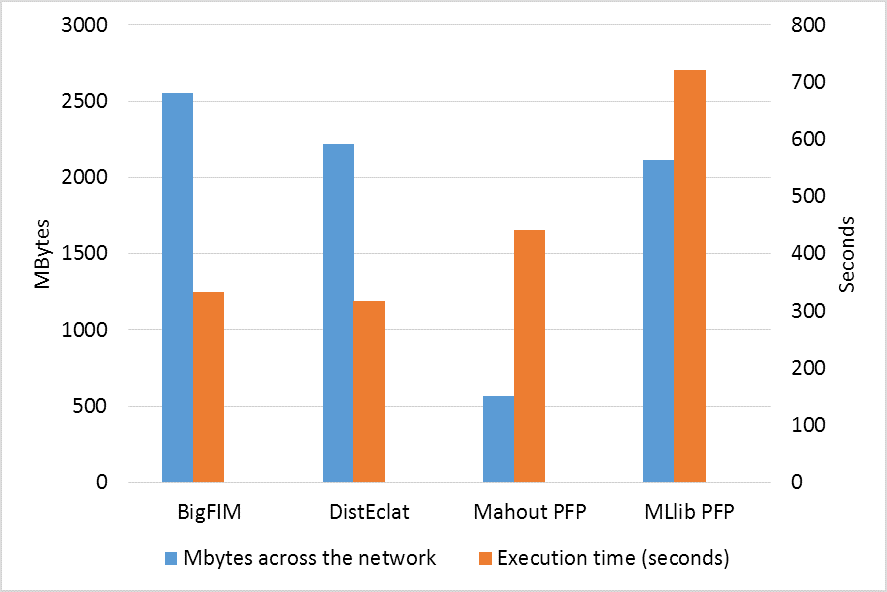
\includegraphics[width=5in]{chapters/survey/immagini/comm_costs.png}
\caption{Communication costs and performance for each algorithm,
Datasets~\#1, $minsup$~0.1\%.
The graph reports an average between transmitted and reveiced data.}
\label{comm_costs}
\end{center}
\end{figure*}

%\begin{table*}[h!]
%\begin{center}
%\caption{Execution times for the experiments in Figure~\ref{comm_costs},
%Datasets~\#1, $minsup$~0.1\%.}
%\label{time_comm_costs}
%\begin{tabular}{|c|c|}
%\hline
%{\bf Algorithm }& {\bf Execution time (seconds)}  \\ \hline
% \hline
%BigFIM & 332\\  \hline
%DistEclat &  317 \\ \hline
%Mahout PFP  &442\\ \hline
%MLlib PFP &  614 \\ \hline
%
%\end{tabular}
%\end{center}
%\end{table*}

\begin{figure*}[!t]
\begin{center}
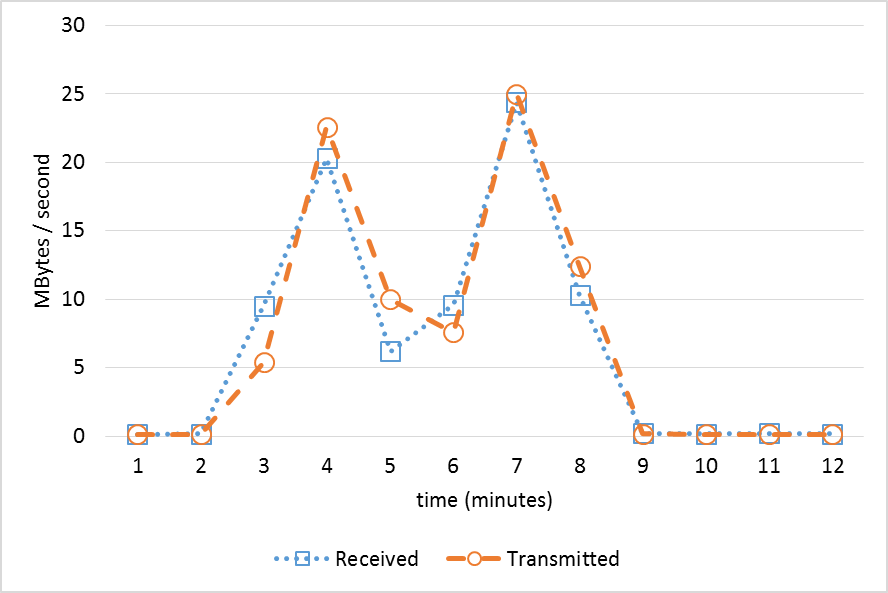
\includegraphics[width=5in]{chapters/survey/immagini/comm_costs_bigfim.png}
\caption{Communication costs of BigFIM, Datasets~\#1, $minsup$~0.1\%.
The graph reports both transmitted and reveiced data.}
\label{comm_costs_bigfim}
\end{center}
\end{figure*}

\begin{figure*}[!t]
\begin{center}
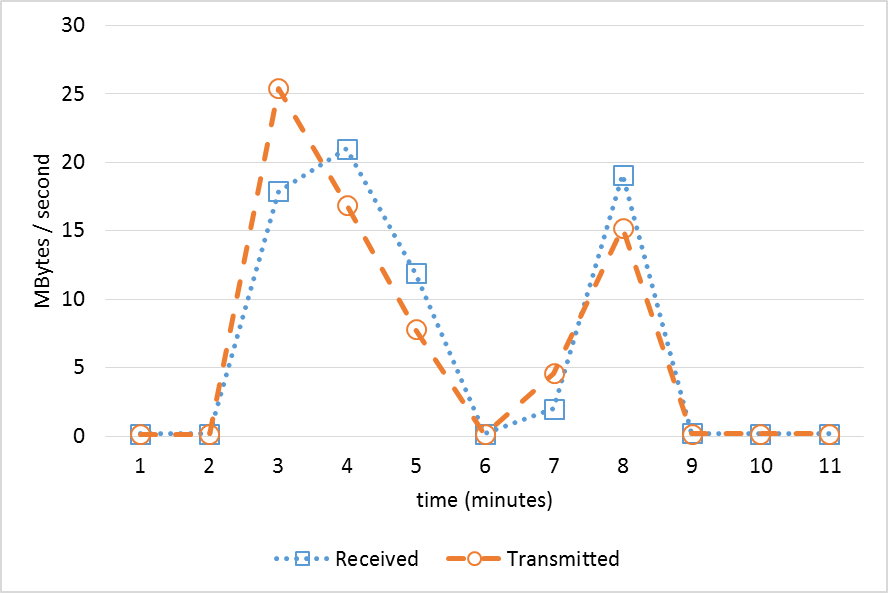
\includegraphics[width=5in]{chapters/survey/immagini/comm_costs_disteclat.png}
\caption{Communication costs of DistEclat, Datasets~\#1, $minsup$~0.1\%.
The graph reports both transmitted and reveiced data.}
\label{comm_costs_disteclat}
\end{center}
\end{figure*}

\begin{figure*}[!t]
\begin{center}
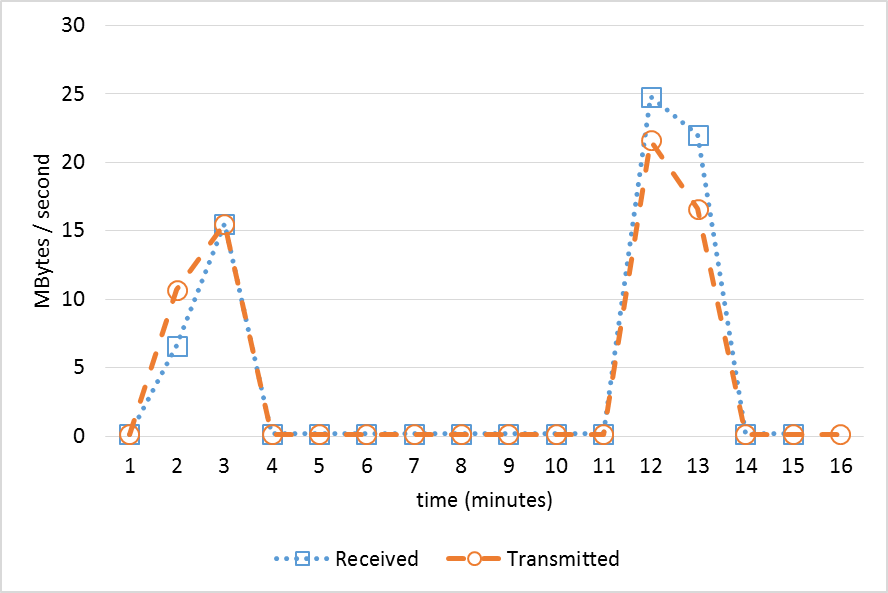
\includegraphics[width=5in]{chapters/survey/immagini/comm_costs_mllib.png}
\caption{Communication costs of MLlib PFP, Datasets~\#1, $minsup$~0.1\%.
The graph reports both transmitted and reveiced data.}
\label{comm_costs_mllib}
\end{center}
\end{figure*}

\begin{figure*}[!t]
\begin{center}
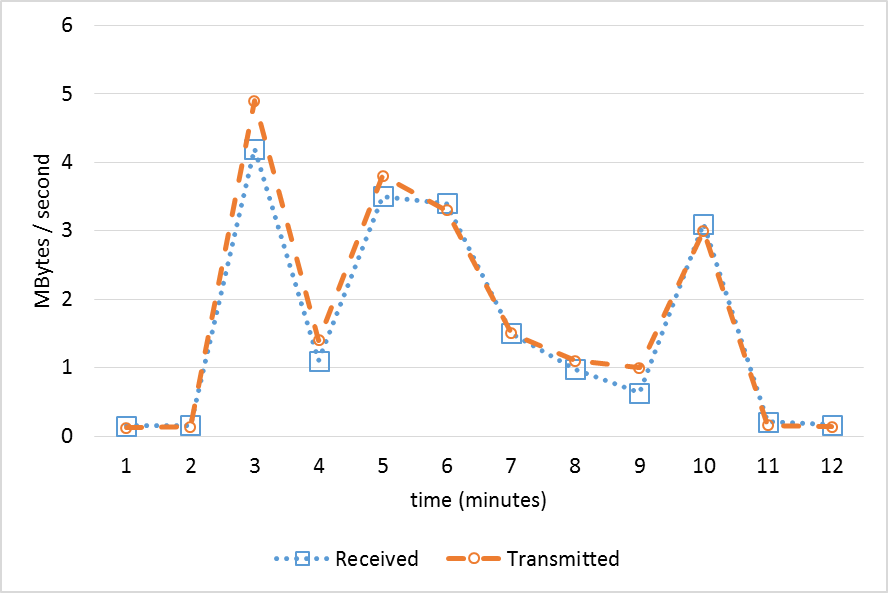
\includegraphics[width=5in]{chapters/survey/immagini/comm_costs_pfp.png}
\caption{Communication costs of Mahout PFP, Datasets~\#1, $minsup$~0.1\%.
The graph reports both transmitted and reveiced data.
}
\label{comm_costs_pfp}
\end{center}
\end{figure*}




Finally, this section presents the experiments addressing the evaluation of
the communication costs.
Specifically, we measure the amount of data transmitted and received
through the nodes network interfaces. This information has been retrieved
by means of the utilities provided by the Cloudera Manager tool.

Experiments have been performed on Dataset~\#1 with a fixed $minsup$ value of 0.1\%,
which was the lowest value for which all algorithms completed the extraction.

Figure~\ref{comm_costs} reports, for each algorithm, the average value
among transmitted and received traffic, compared to the total execution time.
Firstly, the two measures are not correlated:
higher communication costs are associated with low execution times
for BigFIM and DistEclat, whereas MLlib reports both measures with high values.
Mahout PFP has a communication cost 4 to 5 times lower than all the others,
which exchange an average of 2~Gigabytes of data.
Mahout PFP average communication cost is around 0.5~Gigabytes,
which is approximately the dataset size.
Even though Mahout PFP is the most communication-cost optimized implementation,
the very low amount of data sent through the network is related
to the adoption of compression techniques, which lead to higher execution times.
To address this issue,
we measured the communication costs of the first phase of BigFIM and Mahout PFP
in word-count toy application. BigFIM generates into the network an
amount of data more than 5 times larger than Mahout PFP.
However, at the same time, the execution time of BigFIM initial phase is
almost 3 times faster than those of Mahout PFP.

Investigating deeper into the specific algorithm communication-cost analisys,   
Figures~\ref{comm_costs_bigfim},~\ref{comm_costs_disteclat},~\ref{comm_costs_pfp},~\ref{comm_costs_mllib}
show the data exchanged throughout the whole execution time
of each algorithm.

BigFIM and DistEclat, in
Figure~\ref{comm_costs_bigfim},~\ref{comm_costs_disteclat}, have a similar
behaviour, with the communication costs grouped into two main phases.
The first phase is related to the prefix extraction,
while the second one matches the prefix preparation and prefix tree mining.
BigFIM saturates the network link capacity (25~Megabytes/s, corresponding to
a 100~Mbit/s full duplex Ethernet interface) during the second phase peak
at minute 7 for both sent and received data,
whereas DistEclat reaches such point during the first phase at minute 3,
in trasmitted data only.
BigFIM is also continuously exchanging data through the network during the
mining process, whereas DistEclat pauses the network data exchange at minute 6.
% %The choice of doing the main tasks of each job (prefix mining and prefix
% expansion) in the map phase, without a full exploitation of data locality,
% strongly affects communication costs. On the other hand, for instance, Mahout
% PFP first phase, in which the header table is obtained through a basic
% WordCount, each mapper exploits data locality working on its shard of the
% dataset.
Also the MLlib PFP implementation (Figure~\ref{comm_costs_mllib})
presents two phases: differently from BigFIM and DistEclat, the middle ``pause'',
dividing the first shuffling phase and the second materialization phase,
is very long and lasts from minute 4 to minute 11,
it is immediately followed by a peak reaching the network capacity
at minute 12.
Mahout PFP communication costs, instead, (Figure~\ref{comm_costs_pfp})
consists of three phases:
the first is related to the counting part,
the second one corresponds to the mining phase,
while the last one is related to the aggregation of the results.
The peak in network data exchange is as low as 5~Mbytes/s.



%
% %However, interestingly, the behaviour does not affect the execution time of
% this mining experiment, in which the considered implementation is outperformed
% by BigFIM and DistEclat as shown in Table~\ref{time_comm_costs}. The reason is
% partially related to an unfair load balancing, sinche the longest mining task
% lasts more than three times the execution time of the fastest ones.




\section{Lessons learned}
\label{lesson}



The reported experiments provide a wide view of the different behaviours of the
algorithms, dealing with diverse types of problems.
With this section, we aim at supporting the reader
in a conscious choice of the most suitable approach,
depending on the use case at hand.
Pursuing this target, we measured the real-life performance
of the openly-available frequent-pattern mining implementations
for the most popular distributed platforms (i.e., Hadoop and Spark).
They have been tested on many different datasets
characterised by different values of
minimum support ($minsup$),
transaction length (dimensionality),
number of transactions (cardinality),
and dataset density,
besides two real-life use cases.
Perfomance in terms of execution time, load balancing, and communication cost
have been evaluated:
a one-table summary of the results is reported in Table~\ref{all_resume}.
As a result of the described experience,
the following general suggestions emerge:

\begin{itemize}
 \item
 Without prior knowledge of dataset density, dimensionality
 (average transaction length), and cardinality (number of transactions),
 \textbf{Mahout PFP} is the algorithm that best guarantees
 the mining task completion,
 at the expense of longer execution times.
 Mahout PFP is the only algorithm able to always reach the experimental limits.
 Furthermore, it exchanges very few data across the network of the cluster.
 \item
 When the dataset size is small with respect to the available memory,
 \textbf{DistEclat} has proven to be among the fastest approaches,
 and also to be able to reach the lowest experimental $minsup$ values.
 DistEclat experiments showed that it cannot scale for large or
 high-dimensional datasets, but when it can complete the itemset extraction,
 it is very fast.
 \item
 On most real-world use cases, with limited dimensionality
 (up to 60 items per transaction on average), \textbf{MLlib PFP}
 has proven to be the most reasonable tradeoff choice,
 with fast execution times and optimal scalability to very large datasets.
 \item
 Finally, for datasets with a high number of dimensions, \textbf{BigFIM} resulted
 the fastest approach,
 but it cannot cope with $minsup$ values as low as the others.
\end{itemize}

\begin{table*}[h!]
\scriptsize
\begin{center}
\caption{
Summary of the limits identified by the experimental evaluation of the
algorithms (lowest $minsup$, maximum transaction length,
largest dataset cardinality).
The faster algorithm for each experiment is marked in bold.
}
\label{all_resume}
\begin{tabular}{|c|c|c|c|c|}
\hline
& Section \ref{minsup_exp} & Section \ref{minsup_exp} & Section \ref{attributes_exp}& Section  \ref{transaction_exp} \\ \hline
% & Transaction & Transaction& Minsup value: 1\% & Minsup value 0.4 \% \\
% &  length: 10 & length: 30 &  &  \\ \hline
% & 10M transactions & 10M transactions &  10M transactions &  Transaction length 10 \\ \hline
% & Dataset \#1 & Dataset &  Dataset &  Dataset \\ \hline
           & $minsup$ & $minsup$ & transaction  & millions of   \\
           &          &          & length       & transactions  \\ \hline
Mahout PFP & 0.002\% & 0.01\%    & 100          & 100 		\\ \hline
MLlib PFP  & 0.002\% & \textbf{0.01\%}   & 60		& \textbf{100} 	\\ \hline
BigFIM     & 0.1\%   & 0.3\%     & \textbf{100} 	& 100 		\\ \hline
DistEclat  & \textbf{0.002\%}& - 	 & - 		& 1 		\\ \hline
\end{tabular}
\end{center}
\end{table*}

%\begin{table*}[h!]
%\begin{center}
%\caption{Experimental result summary.
%\textbf{@FABIO8: qui secondo me devi fare una colonna per ogni subsection sperimentale,
%es. colonna ``valore minimo di $minsup$, Section X.Y'' e riporti i valori limite,
%ecc. con le altre subsection... cos\`i invece non mi piace, non \`e immediato
%da capire... e poi magari metterei un asterisco sul metodo pi\`u veloce
%(o i due pi\`u veloci se sono molto simili) in ogni colonna.
%Se non \`e chiaro ci sentiamo.}
%}
%\label{all_resume}
%\begin{tabular}{|c|c|c|c|c|}
%\hline
%           & Transaction & Transaction& Minsup value: 1\% & Minsup value 0.4 \% \\
%  &  length: 10 & length: 30 &  &  \\ \hline
%            & 10M transactions & 10M transactions &  10M transactions &  Transaction length 10 \\ \hline
%Algorithm  & Lowest minsup:                           & Lowest minsup:                             & Max. transaction           & Max. number of   \\
%  &                       &                             &  length:           & transactions (millions):   \\ \hline
%Mahout PFP & 0.002 \%                                  & 0.01 \%                                   & 100                                  & 100                                         \\ \hline
%MLlib PFP  & 0.002 \%                                  & 0.01 \%                                   & 60                                   & 100                                         \\ \hline
%BigFIM     & 0.1 \%                                    & 0.3 \%                                    & 100                                  & 100                                         \\ \hline
%DistEclat  & 0.002 \%                                  & -                                         & -                                    & 1                                           \\ \hline
%\end{tabular}
%\end{center}
%\end{table*}






\section{Lessons Learned}
\label{lesson}


The reported experiments provide a wide view of the different behaviours of the
algorithms in various experimental settings.
With this section, we aim at supporting the reader
in a conscious choice of the most suitable approach,
depending on the use case at hand.
Pursuing this target, we measured the real-life performance
of the openly-available frequent-pattern mining implementations
for the most popular distributed platforms (i.e., Hadoop and Spark).
They have been tested on many different datasets
characterized by different values of
minimum support ($minsup$),
transaction length (dimensionality),
number of transactions (cardinality),
and dataset density,
besides two real-life use cases.
Performance in terms of execution time, load balancing, and communication cost
have been evaluated:
a one-table summary of the results is reported in Table~\ref{all_resume}.
As a result of the described experience,
the following general suggestions emerge:

\begin{itemize}
 \item {\bf High reliability.}
 Without prior knowledge of dataset density, dimensionality
 (average transaction length), and cardinality (number of transactions),
 \textbf{Mahout PFP} is the algorithm that best guarantees
 the mining task completion,
 at the expense of longer execution times.
 Mahout PFP is the only algorithm able to always reach the experimental limits.


 \item {\bf High cardinality and low-dimensional data.}
 On most real-world use cases, with limited dimensionality
 (up to 60 items per transaction on average), \textbf{MLlib PFP}
 has proven to be the most reasonable tradeoff choice,
 with fast execution times and optimal scalability to very large datasets.

 \item {\bf High-dimensional data.}
 For high-dimensional datasets, \textbf{BigFIM} resulted
 the fastest approach, but it cannot cope with $minsup$ values as low as the others. In those cases, \textbf{Mahout PFP} represents the only option.

 \item {\bf Limited dataset size.}
 When the dataset size is small with respect to the available memory,
 \textbf{DistEclat} has proven to be among the fastest approaches,
 and also to be able to reach the lowest experimental $minsup$ values.
 DistEclat experiments showed that it cannot scale for large or
 high-dimensional datasets, but when it can complete the itemset extraction,
 it is very fast.

\end{itemize}

%From an even more practical point of view, all the implementations revealed to be quite easy to deploy and use. 
%Actually, the only requirement for all the implementations to be run was the Hadoop/Spark installation 
%(from a single machine scenario to a large cluster). 
%Only the MLlib PFP implementation requires few additional steps, since it is delivered as a library requiring some coding skills: 
%the users should develop their own class and compile it.

\begin{table*}[h!]
\scriptsize
\begin{center}
\caption{
Summary of the limits identified by the experimental evaluation of the
algorithms (lowest $minsup$, maximum transaction length,
largest dataset cardinality).
The faster algorithm for each experiment is marked in bold.
}
\label{all_resume}
\begin{tabular}{|c|c|c|c|c|}
\hline
& Section \ref{minsup_exp} & Section \ref{minsup_exp} & Section \ref{attributes_exp}& Section  \ref{transaction_exp} \\ \hline
% & Transaction & Transaction& Minsup value: 1\% & Minsup value 0.4 \% \\
% &  length: 10 & length: 30 &  &  \\ \hline
% & 10M transactions & 10M transactions &  10M transactions &  Transaction length 10 \\ \hline
% & Dataset \#1 & Dataset &  Dataset &  Dataset \\ \hline
           & $minsup$ & $minsup$ & transaction  & millions of   \\
           &          &          & length       & transactions  \\ \hline
Mahout PFP & 0.002\% & 0.01\%    & \textbf{100 (0.1\%)}          & 100 		\\ \hline
MLlib PFP  & 0.002\% & \textbf{0.01\%}   & 60		& \textbf{100} 	\\ \hline
BigFIM     & 0.1\%   & 0.3\%     & 100 (1\%) 	& 100 		\\ \hline
DistEclat  & \textbf{0.002\%}& - 	 & - 		& 1 		\\ \hline
\end{tabular}
\end{center}
\end{table*}

%\begin{table*}[h!]
%\begin{center}
%\caption{Experimental result summary.
%\textbf{@FABIO8: qui secondo me devi fare una colonna per ogni subsection sperimentale,
%es. colonna ``valore minimo di $minsup$, Section X.Y'' e riporti i valori limite,
%ecc. con le altre subsection... cos\`i invece non mi piace, non \`e immediato
%da capire... e poi magari metterei un asterisco sul metodo pi\`u veloce
%(o i due pi\`u veloci se sono molto simili) in ogni colonna.
%Se non \`e chiaro ci sentiamo.}
%}
%\label{all_resume}
%\begin{tabular}{|c|c|c|c|c|}
%\hline
%           & Transaction & Transaction& Minsup value: 1\% & Minsup value 0.4 \% \\
%  &  length: 10 & length: 30 &  &  \\ \hline
%            & 10M transactions & 10M transactions &  10M transactions &  Transaction length 10 \\ \hline
%Algorithm  & Lowest minsup:                           & Lowest minsup:                             & Max. transaction           & Max. number of   \\
%  &                       &                             &  length:           & transactions (millions):   \\ \hline
%Mahout PFP & 0.002 \%                                  & 0.01 \%                                   & 100                                  & 100                                         \\ \hline
%MLlib PFP  & 0.002 \%                                  & 0.01 \%                                   & 60                                   & 100                                         \\ \hline
%BigFIM     & 0.1 \%                                    & 0.3 \%                                    & 100                                  & 100                                         \\ \hline
%DistEclat  & 0.002 \%                                  & -                                         & -                                    & 1                                           \\ \hline
%\end{tabular}
%\end{center}
%\end{table*}







\section{Open research issues}
\label{openissues}
%
Following the analysis of the state-of-the-art in frequent itemset mining
algorithms for distributed computing frameworks, and the in-depth experimental
evaluation discussed in Section~\ref{experimental},
we can deduce that different efficient and scalable
algorithms have been designed and developed during the last years.
However, despite the technological advancements, there is still room for
improvements. Specifically,
some open problems, summarized below, should be addressed to support
a more effective and efficient data mining process on Big Data collections.

\textbf{Algorithm selection.}
Many algorithms have been proposed in literature
to efficiently extract correlations among data in the form of frequent itemsets,
as discussed in this review.
However, to apply one of the above algorithms for the analysis of a given
dataset, the analyst needs to identify
the best algorithm suitable for her use case,
able to efficiently deal with the
underlying data characteristics.
The selection process is mainly based on the analyst expertise and must be
handpicked for a given dataset.
Thus, innovative and effective techniques that can intelligently and
automatically support the analyst in the identification of the best algorithm
for the current use case analysis are needed.

\textbf{Parameter setting.}
The performance of the available algorithms to extract frequent
itemsets depends on the choice of the input parameters, like the support
threshold, which dramatically impacts the execution time based on the data
distribution characteristics. The optimal trade-off between execution time and
result accuracy must be manually selected for any given application, based on
the
analysts expertise.
To extract meaningful and interesting itemsets while maintaining the
number of extracted results within manageable limits, a large number of
experiments should be performed and the results
manually evaluated by domain experts.
The whole process is time consuming and requires a considerable
amount of effort and skills. Thus, new scalable approaches
capable of self-configuring to automatically extract actionable
knowledge from massive data repositories
are needed.

\textbf{Missing support for really high-dimensional datasets}
The performance analysis have included a mining experiments on datasets with 
up to 100 dimensions. Even if BigFIM has outperformed the competitors, its performances
are still very weak for low minimum support values. On the other hand, 100-features dataset certainly
do not represent a state-of-the-art high dimensional problem, which can be instead characterized by thousands of million of dimensions.
Thus, arises from the review is a concrete lack of a real scalable implementation which focus on the number of
items per transaction. 

\textbf{Full exploitation of computational capabilities of distributed
frameworks.}
Up to now, data mining algorithms have been mainly designed to be
optimized when running on centralized architectures.
Furthermore, recursive primitives cannot be easily translated into
distributed approaches,
thus the efficiency of the current distributed
implementations are limited.
There is room for novel approaches natively
designed to be distributed, able to efficiently address the itemset
mining discovery and to fully exploit computational capabilities of
distributed frameworks.




%Following the analysis of the state-of-the-art in frequent itemset mining
%algorithms for distributed computing frameworks, and the in-depth experimental
%evaluation discussed in Section~\ref{experimental},
%we can deduce that different efficient and scalable
%algorithms have been designed and developed during the last years.
%The review followed a structured analysis. After a theoretical description of the algorithmic design choices
%in terms of exploration and distribution of the search space, we introduced two aspects more related to distributed environment, such as Load Balancing and Communication costs. After this initial theoretical phase, we have largely put to the test all the algorithms in several possible use cases, leveraging both synthetic and real datasets. Indeed, the experiments results, in some cases, did not achieve the expectations related to theoretical analysis. These events allowed us to better understand  the impact of the aforementioned aspects on the final performances and, in general, on distributed frequent itemset mining domain.

%This type of analysis, which is, to our knowledge, unique in the state of the art, allowed us to extract very interesting take-aways and open questions. 

The comparative study presented in this review highlighted interesting research directions to enhance distributed itemset mining algorithms for Big Data.


\textbf{Smarter load balancing techniques.} 
The experimental evaluation allowed us to show that load balancing issues significantly affect distributed itemset mining performance, more than communication and I/O costs (e.g., reading the dataset many times). 
Specifically, the different complexity among the task-level sub-problems leads to load unbalance in the cluster 
(i.e., some sub-problems are more computationally expensive and time consuming than others causing inefficient resource usage).
%the largest sub-problems could be still too complex to be analyzed in a single task causing worse performance or the bottleneck in memory allocation).
Load balancing improvements should be addressed in the design of new distributed frequent itemset mining algorithms. 
In that context, we believe that a new research direction to investigate is the definition of variable-length prefixes, 
with respect to which the mining sub-problems are defined, 
hence leading to a more balanced exploration of the search space. 

%\textbf{Innovative scheduling schema.} 
%{\bf Paolo. Ci\`o che \`e descritto dopo non mi sembra sia un problema di scheduling. Non mi torna. Da discutere.}
%{\bf Paolo. Questa parte va rivista in base a come Elena sta modificando le lettere. Sar\`a molto piu smorzato nelle lettere e quindi bisogna capire come cambiare questo punto.}
%The experiments highlighted the unreliability of approaches optimizing reading phases and communications cost in the sake of performance. In the frequent itemset mining domain, the input datasets are often much smaller than the data structures the algorithms should keep in memory. Given this peculiarity, reading costs hardly dominate the overall performance. 
%The reduction of the communication costs should be addressed in the design of innovative scheduling schema to give a higher priority to appropriate tasks 
%\textbf{PER FABIO: NON HO CAPITO cosa volevate dire. RIESCI A FINIRE LA FRASE?}
%\textbf{Fabio: Non sono d'accordo sull'evoluzione di questo paragrafo. Non so se l'hai trovato già così ma secondo me lo scheduling centra poco. La versione che avevo scritto io forse è troppo prolissa. Forse la versione di Elena nella lettera è equilibrata.. te la cito: the experiments highlighted the unreliability of approaches optimizing reading phases and communications cost in the sake of performance. In the frequent itemset mining domain, the input datasets are often much smaller than the data structures the algorithms should keep in memory. Given this peculiarity, reading costs hardly dominate the overall performance. Hence, a higher priority should be given to an appropriate and balanced handling of the inner structures exploited for the itemsets extraction. }



%However, despite the technological advancements, there is still room for
%improvements. Specifically,
%some open problems, summarized below, should be addressed to support
%a more effective and efficient data mining process on Big Data collections.



\textbf{Self-tuning itemset mining frameworks.} 
As discussed in the paper, different algorithms have been proposed in literature
to discover frequent itemsets. 
However, the efficient exploitation of each algorithm strongly depends on specific skills and expertise. 
The analyst is required to select the best method to efficiently deal with the
underlying data characteristics, 
and manually configure it 
(e.g., from input parameters settings, such as the $minsup$ threshold, the $k$ parameter of BigFIM, etc., to distributed frameworks tuning).
%The optimal trade-off between execution time and
%result accuracy {\bf Paolo. Cos'è l'accuracy per gli itemset?} must be manually selected for any given application, based on
%the analysts expertise.
Thus, state-of-the-art algorithms may become ineffective because of the inefficient hand-picked choices 
of the inappropriate specific implementations, and cumbersome parameter-configuration sessions.
The improvements in algorithm usability should be addressed by designing innovative self-tuning itemset mining 
frameworks, capable of intelligently selecting the most appropriate itemset extraction algorithm 
and automatically configuring it.



% \textbf{Full exploitation of computational capabilities of distributed frameworks.}
% Up to now, data mining algorithms have been mainly designed to be optimized when running on centralized architectures.
% Furthermore, recursive primitives cannot be easily translated into distributed approaches,
% thus the efficiency of the current distributed implementations are limited.
% There is room for novel approaches natively designed to be distributed, able to efficiently address the itemset
% mining discovery and to fully exploit computational capabilities of distributed frameworks.



\section{Relevant Pubblications}


D.~Apiletti, P.~Garza, and F.~Pulvirenti, ``A review of scalable approaches for
  frequent itemset mining,'' in \emph{East European Conference on Advances in
  Databases and Information Systems}.\hskip 1em plus 0.5em minus 0.4em\relax
  Springer International Publishing, 2015, pp. 243--247.

D.~Apiletti, T.~Baralis, Elena~Cerquitelli, P.~Garza, and F.~Pulvirenti,
  ``Frequent itemsets mining for big data: an experimental analysis,''
  \emph{Submitted to Big Data Research - Under Review}.


\chapter {Frequent Itemset Mining for High-Dimensional data}\label{pampa}

\section{Introduction}
\label{Introduction}
In the last years, the increasing capabilities of recent applications
to produce and store huge amounts of information,
the so called "Big Data"~\cite{Jin201559}, have changed dramatically
the importance of the intelligent analysis of data.
Data mining, together with machine learning~\cite{DBLP:journals/bdr/Al-JarrahYMKT15}, 
is considered
one of the fondamental tools on which Big Data analytics
are based.
In both academic and industrial domains, the interest towards data mining,
which focuses on extracting effective and usable knowledge from large
collections of data, has risen.
The need for efficient and highly scalable data mining tools increases with the
size of the datasets,
as well as their value for businesses and researchers aiming at extracting
meaningful insights increases.\\
Frequent (closed) itemset mining is among the most complex exploratory
techniques in data mining.
It is used to discover frequently co-occurring items
according to a user-provided frequency threshold, called minimum support.
Existing mining algorithms revealed to be very efficient on simple datasets
but very resource intensive in Big Data contexts.
In general, the application of data mining techniques to Big Data collections
is characterized by the need of huge amount of resources.
For this reason, we are witnessing the explosion of parallel and distributed
approaches,
typically based on distributed frameworks, such as Apache Hadoop~\cite{HDFS}
and Spark~\cite{Zaharia_spark}.
As clearly shown in Chapter \ref{survey}, unfortunately, most of the scalable distributed techniques
for frequent itemset mining have been designed to cope with datasets
characterized by few items per transaction (low dimensionality, short
transactions). Their design, on the contrary, focuses on very large datasets in terms of number of
transactions.
Currently, only single-machine implementations exist to address very long
transactions,
such as Carpenter~\cite{Zaki_Carpenter}, and no distributed implementations at
all.\\
%Nevertheless, many researchers in scientific domains such as bioinformatics or
%networking,
%often require to deal with this type of data.
Nevertheless, many scientific applications, such as bioinformatics or networking, 
generate a large number of events characterized by a variety of features.
Thus, high-dimensional datasets have been continuosly generated.
For instance, most gene expression datasets are characterized by
a huge number of items (related to tens of thousands of genes)
and a few records (one transaction per patient or tissue).
Many applications in computer vision deal with high-dimensional data, such as
face recognition.
An increasing portion of big data is actually related to geospatial data~\cite{Lee201574} and
smart-cities. Some studies have built this type of large datasets
measuring the occupancy of different car lanes:
each transaction describes the occupancy rate in a captor location and in a
given timestamp~\cite{PEMSDataset}.
In the networking domain, instead,
the heterogeneous environment provides many different datasets
characterized by high-dimensional data,
such as URL reputation, advertising, and social network
datasets~\cite{snapnets}.
To effectively deal with those high-dimensional datasets,
novel and distributed approaches are needed.

This work introduces PaMPa-HD \cite{pampa_v1}, \cite{pampa_pulvi},
a parallel MapReduce-based frequent closed itemset mining algorithm
for high-dimensional datasets.
PaMPa-HD relies on the Carpenter algorithm~\cite{Zaki_Carpenter}. 
The PaMPa-HD design\footnote{The source code of PaMPa-HD can be downloaded from https://github.com/fabiopulvi/PaMPa-HD},through an ad-hoc synchronization technique, takes into account crucial design aspects,
such as load balancing and robustness to memory-issues. Furthermore, different strategies have been proposed to easily tune up the parameter configuration.
The algorithm has been thoroughly evaluated on real high dimensional datasets. 
PaMPa-HD outperforms the state-of-the-art distributed approaches
in execution time and by supporting lower minimum support threshold. 


The paper is organized as follows:
Section~\ref{Preliminaries} briefly reintroducess the frequent (closed) itemset mining
problem,
Section~\ref{Carpenter algorithm} briefly describes the centralized version
of Carpenter,
and Section~\ref{Distributed implementation outline} presents the proposed
PaMPa-HD algorithm.
Section~\ref{Experiments} describes the experimental evaluations
proving the effectiveness of the proposed technique,
Section~\ref{Applications} discusses possible applications of PaMPa-HD and, finally, Section~\ref{Conclusion} introduces future works and conclusions.
%Section~\ref{Related work} presents a brief review of the state of the art,
%and Section~\ref{Applications} discusses possible applications of PaMPa-HD.
%Finally, Section~\ref{Conclusion} introduces future works and conclusions.





\section{Frequent itemset mining background}
\label{Preliminaries}

\begin{figure}[!t]
%\renewcommand{\arraystretch}{1.3}
%\centerline
{\subfloat[Horizontal representation of $\mathcal{D}$]{
\label{horizontalexampledataset}
\begin{tabular}{|c|l|}
\hline
\multicolumn{2}{|c|}{$\mathcal{D}$}\\
\hline
\hline
	tid & items \\
\hline
	1 & a,b,c,l,o,s,v \\
\hline
	2 & a,d,e,h,l,p,r,v \\
\hline
	3 & a,c,e,h,o,q,t,v \\
\hline
	4 & a,f,v \\
\hline
	5 & a,b,d,f,g,l,q,s,t \\
\hline
\end{tabular}}}%
\hfil
{\subfloat[Transposed representation of $\mathcal{D}$]{
\label{TTexampledataset}
\begin{tabular}{|l|l|}
\hline
\multicolumn{2}{|c|}{$TT$}\\
\hline
\hline
	item & tidlist \\ \hline
	a & 1,2,3,4,5 \\ \hline
	b & 1,5 \\ \hline
	c & 1,3 \\ \hline
	d & 2,5 \\ \hline
	e & 2,3 \\ \hline
	f & 4,5 \\ \hline
	g & 5 \\ \hline
	h & 2,3 \\ \hline
	l & 1,2,5 \\ \hline
	o & 1,3 \\ \hline
	p & 2 \\ \hline
	q & 3,5 \\ \hline
	r & 2 \\ \hline
	s & 1,5 \\ \hline
	t & 3,5 \\ \hline
	v & 1,2,3,4 \\ \hline
\end{tabular}}}%
\hfil
{\subfloat[$TT|_{\{2,3\}}$: example of con\-di\-tio\-nal
tran\-spo\-sed table]{
\label{conditionalexampledataset}
\begin{tabular}{|l|l|}
\hline
\multicolumn{2}{|c|}{$TT|_{\{2,3\}}$}\\
\hline
\hline
item & tidlist \\ \hline
a &4,5 \\ \hline
e & - \\ \hline
h & -\\ \hline
v &4 \\ \hline
\end{tabular}}}%
\caption{Running example dataset $\mathcal{D}$}
\label{exampledataset}
\end{figure}
%
%Let $\mathcal{I}$ be a set of items. A transactional dataset $\mathcal{D}$
%consists of a set of transactions $\{t_1, \dots, t_n\}$,
%where each transaction $t_i\in \mathcal{D}$ is a set of items (i.e.,
%$t_i\subseteq \mathcal{I}$)
%and it is identified by a transaction identifier ($tid_i$).
%Figure~\ref{horizontalexampledataset} reports an example of a transactional
%dataset with 5 transactions.
%It is used as a
%running example through the paper.
%
%An itemset $I$ is defined as a set of items (i.e., $I\subseteq\mathcal{I}$) and
%it is characterized by a tidlist and a support value.
%The tidlist of an itemset $I$, denoted by $tidlist(I)$, is defined as the set of
%tids of the transactions in $\mathcal{D}$ containing $I$,
%while the support of $I$ in $\mathcal{D}$, denoted by $sup(I)$, is defined as
%the ratio between the number of transactions in $\mathcal{D}$ containing $I$
%and the total number of transactions in $\mathcal{D}$ (i.e.,
%$|tidlist(I)|/|\mathcal{D}|$).
%For instance, the support of the itemset \textit{\{aco\}} in
%the running example dataset $\mathcal{D}$ is 2/5 and its tidlist is $\{1,3\}$.
%An itemset $I$ is considered frequent if its support is greater than a
%user-provided minimum support threshold $minsup$.
%
%Given a transactional dataset $\mathcal{D}$ and a minimum support threshold
%$minsup$, the Frequent Itemset Mining \cite{KumarBook} problem consists in
%extracting the complete set of frequent itemsets from $\mathcal{D}$.
%In this paper, we focus on a valuable subset of frequent itemsets called
%frequent closed itemsets~\cite{Zaki_Carpenter}. Closed itemsets
%allow representing the same information of traditional frequent itemsets in a
%more compact form.
%In addition, an item or itemset $I$ is closed in  $\mathcal{D}$ if there exists no superset that
%has the same support count as  $I$.\\
%For instance, in our running example, given a $minsup=2$, the itemset \textit{\{ab\}} is a frequent itemset (support=2), but it is not closed for the presence of the itemset \textit{\{abls\}} (support=2). 
%% %If an itemset is frequent, all of its subsets are frequent for the
%% \textit{monotonic property}.
%% %For the same rule, if an items or an itemset is not frequent, none of its
%% supersets are frequent. In addition, an items
%% % or itemset $I$ is closed in  $\mathcal{D}$ if there exists no superset that
%% has the same support count as  $I$.\\
Since Frequent Itemset Mining preliminaries were introduced far before in the dissertation,
let us just recall and deepen the key concepts fundamental to better understand PaMPa-HD and its
enumeration tree-based exploration strategy.

As already mentioned, a transactional dataset can also be represented in a vertical format, which is
usually a more effective representation of the dataset when the average number
of items per transactions is orders of magnitudes larger than the number of
transactions.
This representation, called \textit{transposed table} $TT$, assumes that each
row consists of an item $i$ and its list of transactions, i.e.,
$tidlist(\{i\})$. Let $r$ be an arbitrary row of $TT$, $r.tidlist$ denotes the
tidlist of row $r$.
Figure~\ref{TTexampledataset} reports the transposed representation of the
running example reported in Figure~\ref{horizontalexampledataset}.

Given a transposed table $TT$ and a tidlist $X$, the conditional transposed
table of $TT$ on the tidlist $X$, denoted
by $TT|_{X}$, is defined as a transposed table such that:
(1) for each row $r_i\in TT$ such that $X\subseteq r_i.tidlist$ there exists one
tuple $r_i^{\prime}\in TT|_{X}$ and
(2) $r_i^{\prime}$ contains all tids in $r_i.tidlist$ whose tid is higher than
any tid in $X$.
For instance, consider the transposed table $TT$ reported in
Figure~\ref{TTexampledataset}. The
projection of $TT$ on the tidlist \textit{\{2,3\}} is the transposed table
reported in Figure~\ref{conditionalexampledataset}.
Each transposed table $TT|_{X}$ is associated with an itemset composed by the
items in $TT|_{X}$.
For instance, the itemset associated with $TT|_{\{2,3\}}$ is \textit{\{aehv\}}
(see Figure~\ref{conditionalexampledataset}).


% %Given a row or a set of rows (in the sequel, \textit{row set}) $x$, $TT|_{x}$,
% is the projection of the whole vertical datasets on the row set x. Each
% transposed table is associated with an itemset composed of the items in the
% table. For each item, the associated tidlist is composed of the tids greater
% than any tid in the row set x. For instance, $TT|_{2,3}$ in tab 3 is the
% transposed table of the row set \textit{2,3} and it represents the itemset
% \textit{aehv}.




\section{The Carpenter algorithm}
\label{Carpenter algorithm}
%As discussed in section \ref{Related work}, t
The most popular techniques to perform itemset mining (e.g.,
Apriori~\cite{Agr94} and FP-growth~\cite{Han00}) adopt the itemset enumeration
approach (see Section \ref{survey_centralized} for further discussion).
% to mine the frequent itemsets.
However, itemset enumeration revealed to be ineffective with datasets with a
high average number of items per transactions \cite{Zaki_Carpenter}.
%Apriori algorithm, in fact, has a very high number of candidates to generate
%and to count, while the trees generated by FP-Growth-based approaches hardly
%fit in main memory.
%In conclusion, these algorithms were not developed for the use cases related
% to high number of features, focusing on high number of transactions.\\
To tackle this problem, the Carpenter algorithm~\cite{Zaki_Carpenter} was
proposed.
Specifically, Carpenter is a frequent itemset extraction algorithm devised to
handle datasets characterized by a relatively small number of
transactions but a huge number of items per transaction.
To efficiently solve the itemset mining problem, Carpenter adopts an effective
depth-first transaction enumeration approach based on the transposed
representation of the input dataset.
To illustrate the centralized version of Carpenter, we will use the running
example dataset $\mathcal{D}$ reported in Figure~\ref{horizontalexampledataset},
and
more specifically, its transposed version (see Figure~\ref{TTexampledataset}).
%Before going deeper into the algorithm explanation, some preliminary
% information will be provided to facilitate the reader comprehension.
%Let us start saying that the algorithm assumes to process a vertical
%transposition of the input dataset.
%Carpenter assumes to process a transposed representation of the input dataset.
Recall that in the transposed
representation each row of the table consists of an item $i$ with its tidlist.
For instance,
the last row of Figure~\ref{TTexampledataset} shows that item \textit{v}
appears in
transactions 1, 2, 3, 4.
%The rows are sorted in a numerical order (oppure The tids in each tidlist are
%sorted in a numerical orders?).
%From the initial transposed table TT, given x as a row or a row set,
%  $x$, $TT|_{x}$, is the projection of the whole vertical datasets on the
%row or the row set $x$, as defined in section \ref{Preliminaries}.\\


\begin{figure}[!t]
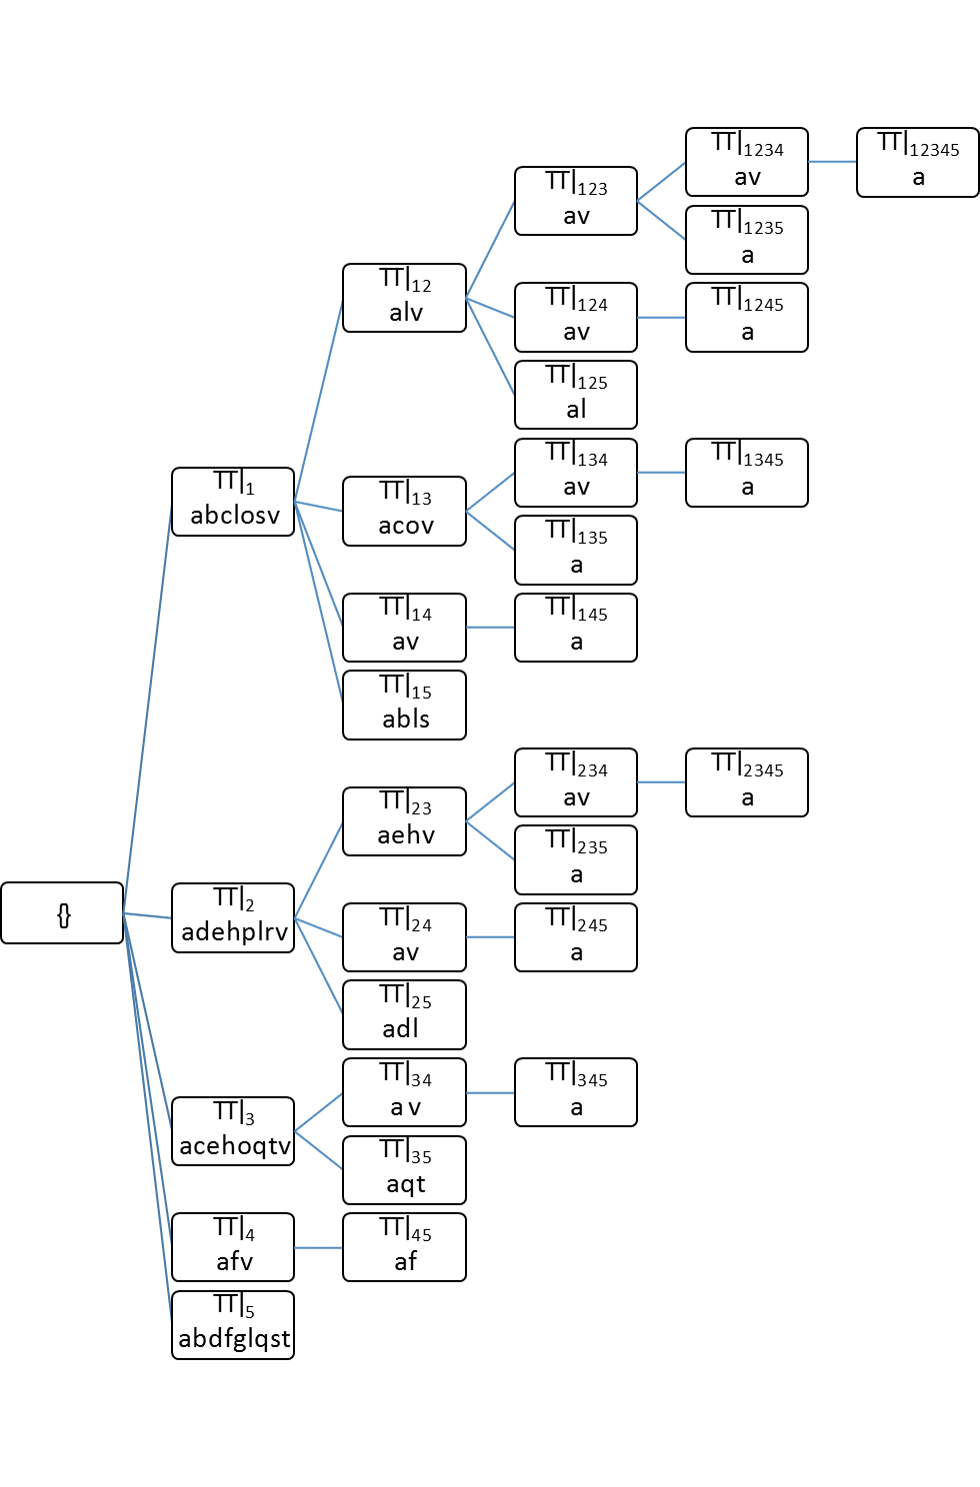
\includegraphics[width=4in]{chapters/pampa/running_example1.png}
\caption{The transaction enumeration tree of the running example dataset in
Figure~\ref{horizontalexampledataset}. For the sake of clarity, no pruning rules
are applied to the tree.}
\label{running_1}
\end{figure}

%Conditional transposed tables and the depth first enumeration of the
%transactions are the core of Carpenter. Specifically,
Basically, Carpenter builds a transaction enumeration tree by exploiting a set of pruning rules
which avoid the expansion of useless branch of the tree. 
In the tree, each node corresponds to a
conditional transposed table $TT|_X$ and its related information (i.e., the
tidlist $X$ with respect to which the conditional transposed table is built and
its associated itemset).
The transaction enumeration tree, when pruning techniques are not applied,
contains all the tid combinations (i.e., all the possible
tidlists $X$).
Figure~\ref{running_1} reports the
transaction enumeration tree obtained by processing the running example dataset.
To avoid the generation of duplicate
tidlists, the transaction enumeration tree is built by exploring the tids in
lexicographical order (e.g., $TT|_{\{1,2\}}$ is generated instead of
$TT|_{\{2,1\}}$).
Each node of the tree is associated with a conditional transposed table on a
tidlist.
For instance, the conditional transposed table
$TT|_{\{2,3\}}$ in Figure~\ref{conditionalexampledataset}, matches the node
$\{2,3\}$ in Figure~\ref{running_1}.


%The enumeration tree is built from initial transposed table: in figure
%\ref{running_1}, a full exploration of the tree based on initial transposed
%table is shown. Each node of the tree, as already said, matches a transposed
%table over a row set. In our example, the transposed table$TT|_{2,3}$ in
%figure 3, matches the node 2,3 in figure \ref{running_1}.
Carpenter performs a depth first search (DFS) of the enumeration tree to mine the set
of frequent closed itemsets.
%Visiting the tree in this way, adopting a pruning branch policy that will
%be detailed in the following, leads to the extraction of the complete
%frequent closed itemset set without duplicates (details and proofs can be
%found in \cite{Zaki_Carpenter}).
%We will describe the Carpenter algorithm by means of the running example.
Referring to the tree in Figure~\ref{running_1}, the depth first search would
lead to the visit of the nodes in the following order:
\{1\}, \{1,2\}, \{1,2,3\}, \{1,2,3,4\}, \{1,2,3,4,5\}, \{1,2,3,5\}, \{...\}.
For each node, Carpenter applies a procedure that decides if the itemset
associated with that node is a frequent closed itemset or not.
%Specifically, for each node, Carpenter decides if the itemset associated with
%the current node is a frequent closed  itemset
%by considering: 1) the tidlist $X$ associated with the node, 2) the conditional
%transposed table
%$TT|_{X}$, 3) the set of frequent closed itemsets found up to the current step
%of the tree search, and 4) the enforced minimum support threshold ($minsup$).
%The first information is useful to enforce the DFS exploration and to check the 
%actual support of the itemset; the conditional transposed table is used to obtain
% the itemset associated to the node, while the remaing tids are useful to determine
% how and if the node should be expanded. The frequent closed itemsets found (3)
% are used to avoid to process the same itemset twice; due to the enumeration tree 
%architecture, the real support of the itemset is the one obtained the first time the 
%itemset is processed in a DFS exploration manner. Finally, the enforced minsup 
%support threshold is used to decide if the itemset is a frequent closed itemset.
Specifically, for each node, Carpenter decides if the itemset associated with
the current node is a frequent closed  itemset
by considering: \begin{enumerate}
\item The tidlist $X$ associated with the node, useful to enforce the depth-first exploration and to check the actual support of the itemset
\item The conditional transposed table $TT|_{X}$, used to obtain the itemset associated to the node and, through the remaing tids, determine how and if the node should be expanded
\item The set of itemsets found up to the current step of the tree search, used to avoid to process the same itemset twice (due to the enumeration tree architecture, the real support of the itemset is the one obtained the first time the itemset is processed in a depth-first exploration manner)
\item The enforced minimum support threshold ($minsup$), used to decide if the itemset is a frequent closed itemset
\end{enumerate}
Based on the theorems reported in~\cite{Zaki_Carpenter}, if the itemset $I$
associated with the current node is a frequent closed itemset then $I$
is included in the frequent closed itemset set. Moreover, by exploiting the
analysis performed on the current node, part of the remaining search space
(i.e.,
part of the enumeration tree) can be pruned, to avoid the analysis of nodes that
will never generate new closed itemsets.
To this purpose, three pruning rules are applied on the enumeration tree, based
on the evaluation performed on the current node and the associated
transposed table $TT|_{X}$:
\begin{itemize}
\item \textbf{Pruning rule 1.} If the size of $X$, plus the number of distinct
tids in the rows of $TT|_{X}$ does not reach the minimum support threshold,
the subtree rooted in the current node is pruned.
\item \textbf{Pruning rule 2.} If there is any tid $tid_i$ that is present in
all the tidlists of the rows of $TT|_{X}$, $tid_i$ is deleted from $TT|_{X}$.
The number of discarded tids is updated to compute the correct support of the
itemset associated with the pruned version of $TT|_{X}$.
\item \textbf{Pruning rule 3.} If the itemset associated with the current node
has been already encountered during the depth first search,
the subtree rooted in the current node is pruned because it can never generate
new closed itemsets.
\end{itemize}

%Rule 3 is the most effective pruning rule, especially considering the
%distributed implementation detailed in \ref{Distributed implementation
%outline}. It allows to prune the branches related to already found itemsets,
%that represents a waste of computation time and memory.
%After the pruning phase, the support of the itemset is compared with the
%minsup. The support is identified by the number of row ids composing $X$,
%plus the number of rows discarded by the second pruning rule. If the support
%is greater or equal than the minsup, as shown in figure 5, the itemset
%is added to the set of frequent closed ones.

The tree search continues in a depth first fashion moving on the next node of
the enumeration tree. More specifically,
let $tid_l$ be the lowest tid in the tidlists of the current $TT|_{X}$, the next
node to explore is the one associated with
$X^\prime=X\cup \{tid_l\}$.


Among the three rules mentioned above, pruning rule 3 assumes a global knowledge
of the enumeration tree explored in a depth first manner.
This, as detailed in section~\ref{Distributed implementation outline}, is very
challenging in a distributed environment that adopts a shared-nothing
architecture, like the one we address in this work.



% %versione 2
% %\\
% %Carpenter algorithm is based on the depth first exploration of a row
% enumeration tree. A running example of the enumeration tree built on the dataset
% in table 1 is represented in figure \ref{running_1}. A transposed table
% $TT|_{x}$ is the projection of the whole vertical datasets on the row set x, as
% defined in \ref{Preliminaries}. Each transposed table is associated with an
% itemset composed of the items in the table. For each item, the associated
% tidlist is composed of the tids greater than any tid in the row set x. Each
% table represents a node in the row enumeration tree. For instance, $TT|_{2,3}$
% in tab 3 corresponds to the node 2 3 in the enumeration tree.
% %\\The tree exploration corresponds to a recursive processing of the transposed
% tables, generating adding a tid to the row set in depth first manner. Exploring
% the tree in this way, applying a set of pruning rules detailed in a few lines,
% leads to the extraction of all the closed itemsets (details and proofs can be
% found in \cite{Zaki_Carpenter}). The first iteration processes the whole
% vertical dataset. Each iteration, given a transposed table $TT|_{x}$ as input,
% can be resumed in:
% %\begin{enumerate}
% %\item apply pruning rules
% %\item if the support is over the minsup, add the related itemset to the set of
% frequent closed itemsets
% %\item expand the table adding a tid in the row set, following a depth first
% manner
% %\item start a new recursion with the new table
% %\end{enumerate}
% %The pruning rules allow to prune some branches without exploring all the
% possible tid combinations. The most effective is the rule used to prune some
% branches of the tree if the related itemsets have already been found in the tree
% exploration. The rules are:
% %\begin{itemize}
% %\item \textbf{Pruning rule 1:} If the row of the projection, plus the potential
% rows in the tid lists do not reach the minimum support threshold, the table is
% discarded and the branch is pruned.
% %\item \textbf{Pruning rule 2:} If there is any row id which is present in all
% the tid lists, it is deleted from the table. The number of discarded rows is
% updated.
% %\item \textbf{Pruning rule 3:} If the itemset characterizing the table has been
% already seen in the tree, the branch is pruned.
% %\end{itemize}
% %The process continues recursively until there is no table to expand and all the
% closed itemsets have been found. A most detailed explanation and theoretical
% proofs are in \cite{Zaki_Carpenter}.

\begin{figure}[!t]
%\centering
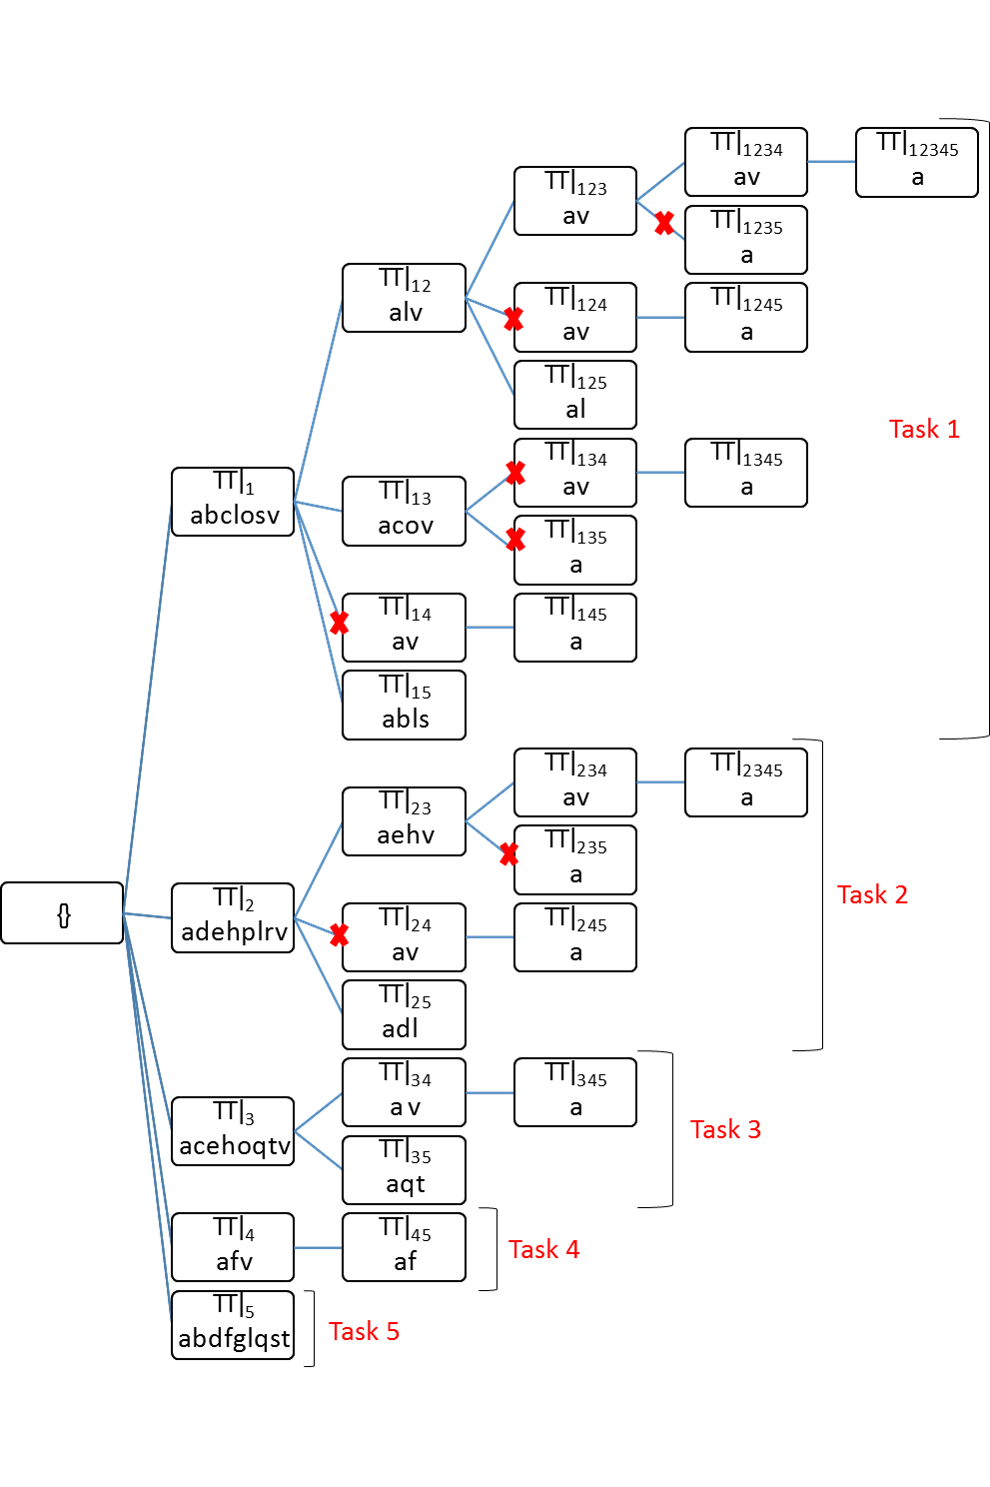
\includegraphics[width=4in]{chapters/pampa/running_example2_d.png}
% where an .eps filename suffix will be assumed under latex,
% and a .pdf suffix will be assumed for pdflatex; or what has been declared
% via \DeclareGraphicsExtensions.
\caption{Running toy example: each node expands a branch of the tree
independently. For the sake of clarity, pruning rule 1 and 2 are not applied. The pruning rule 3 is
applied only within the same task: the small crosses on the edges represent pruned
nodes due to local pruning rule 3, e.g.
the one on node \{2 4\} represents the pruning of node \{2 4\}.}
\label{running_2}
\end{figure}




\section{The PaMPa-HD algorithm}
\label{Distributed implementation outline}
In this section we describe the new algorithm, called PaMPa-HD, proposed in this paper. Specifically, 
we describe how PaMPa-HD parallelizes the itemset mining
process and applies the pruning rules discussed in Section~\ref{Carpenter algorithm} in a parallel 
environment.
Furthermore, we discuss how, through an ad-hoc
synchronization phase, PaMPa-HD achieves a good load balancing
and robustness to memory issues.

As discussed in the previous section, given the complete enumeration tree (see Figure~\ref{running_1}), the
centralized Carpenter algorithm
extracts the whole set of closed itemsets by performing a depth first search
(DFS) of the tree.
%By tracing the set of closed itemsets encountered by traversing the tree,
%Carpenter also prunes part of the search space by applying the three pruning
%rules illustrated above. 
%described in Section~\ref{Carpenter algorithm}.
Differently, in order to parallelize the mining process, the PaMPa-HD algorithm splits the depth
first search process in a set of (partially) independent
sub-processes, that autonomously evaluate sub-trees of the search space.
%PaMPa-HD exploits the pruning rules 1 and 2 and a slight variation of the 
%pruning rule 3 discussed in Section~\ref{Carpenter algorithm}.
Specifically, the whole problem can be split by assigning
each subtree rooted in $TT|_{X}$, where $X$ is a single transaction id in the
initial dataset, to an independent sub-process.
Each sub-process applies the centralized version of Carpenter on its conditional
transposed table $TT|_{X}$ and extracts a subset of the final closed itemsets.
The subsets of closed itemsets mined by each sub-process
are merged to compute the whole closed itemset result.
Since the sub-processes are independent, they can be executed in parallel by
means of a distributed computing platform, e.g., Hadoop.
Figure~\ref{running_2} shows the application of the proposed approach on the
running example.
Specifically, five independent sub-processes are executed in the case of the
running example, one for each row (transaction) of the original dataset.
The crosses on the nodes represent the local pruning within each parallel task.
Partitioning the enumeration tree in sub-trees allows processing bigger
enumeration trees with respect to the centralized version. However, this
approach does not allow fully exploiting pruning rule 3
because each sub-process works independently and is not aware of the partial
results (i.e., closed itemsets) already extracted by the other sub-processes.
Hence, each sub-process can only prune part of its own search space by
exploiting its ``local'' closed itemset list, while
it cannot exploit the closed itemsets already mined by the other sub-processes.
For instance, Task T2 in Figure~\ref{running_2} extracts the closed itemset $av$
associated with node $TT|_{2, 3, 4}$.
However, the same closed itemset is also mined by T1 while evaluating node
$TT|_{1, 2, 3}$.
In the centralized version of Carpenter, the duplicate version of $av$
associated with node $TT|_{1, 2, 4}$ is not generated because $TT|_{1, 2, 4}$
follows
$TT|_{1, 2, 3}$ in the depth first search, i.e., the tasks are serialized and
not parallel.

Since pruning rule 3 has a high impact on the reduction of the search space, its
inapplicability leads to a negative
impact on the execution time of the distributed algorithm (see Section~\ref{Experiments} for further details).
To address this issue, we share partial results among the sub-processes.
Each independent sub-process analyzes only a part of the search subspace.
Then, when a maximum number of visited nodes is reached, the partial results are
synchronized through a synchronization phase. Of course, the exploration of the
tree finishes also when the subspace has been completely explored.
%Each sub-process analyzes only a part the search subspace, then, when memory is
%full or when a maximum number of visited nodes is reached, it stores on disk
%(e.g., in HDFS, the Hadoop distributed file system) the partial set of closed
%itemset mined so far and the remaining sub-tree left to analyze.

Specifically, the sync phase filters the partial results (i.e., nodes of the tree
still to be analyzed and found closed itemsets) globally applying pruning rule
3. The pruning strategy consists of two phases.
In the first one, all the transposed tables and the already found closed
itemsets are analyzed. The transposed tables and the closed itemsets related to
the same itemset are grouped together in a bucket. For instance, in our running
example, each element of the bucket $B_{av}$ can be:
\begin{itemize}
\item a frequent closed itemset $av$ extracted during the subtree exploration of
the node $TT_{3, 4}$,
\item a transposed table associated to the itemset $av$ among the ones that
still have to be expanded (nodes  $TT_{1, 2, 3}$ and  $TT_{2, 3, 4}$).
\end{itemize}
We remind the readers that, because of the independent nature of the Carpenter
subprocesses, the elements related to the same itemset can be numerous, because
obtained in different subprocesses. Please note that all the extracted closed
itemsets come together with the tidlist of the node in which they have been
extracted.

In the second phase, in order to respect the depth-first pruning strategy of the
rule 3, for each bucket it is kept only the oldest element (transposed table or
closed itemset) based on a depth-first order. The depth-first sorting of the
elements can be easily obtained comparing the tidlists of the elements of the
bucket.
Therefore, in our running example from the
bucket $B_{av}$, it is kept the node $TT_{1, 2, 3}$ (See Figure~\ref{running_3b}) .
The transposed tables which are not pruned in this phase are then expanded to continue the enumeration tree exploration.


Afterwards, a new set of sub-processes is defined from the filtered results,
starting a new iteration of the algorithm. In the new iteration, the Carpenter
tasks process also the frequent closed itemsets obtained in the previous iteration,
which are used to enrich the local memory of the task and enhance the effectiveness of the local pruning. 
The Carpenter tasks
process the remaining transposed tables, that are expanded, as before, until the
maximum number of processed tables is reached. In order to enhance the
effectiveness of the pruning rules related to the local Carpenter task, the
tables are processed in a depth-first order. After that, as before, in the
synchronization phase, pruning rule 3 is applied.
%A synchronization and pruning task works on the partial results
%of the sub-processes to globally apply pruning rule 3
%on the remaining search subspaces, i.e.,
%on the remaining nodes of the enumeration tree.
%After the application of the synchronization and pruning step,
%a new set of sub-processes is defined,
%for each remaining node of the enumeration tree.
%that is a descendant of one of the nodes analyzed during the first iteration a
%new process is instantiated and executed.
The overall process is applied iteratively by instantiating new sub-processes
and synchronizing their results,
until there are no nodes left.
The application of this approach to our running example is represented in
Figure~\ref{running_3}, in which the small crosses represent the pruning related to the local
state memory; and in Figure~\ref{running_3b}, in which the bigger crosses represent the pruning related to the synchronization phase.
The table related to the itemset \textit{av}
associated with the tidlist/node \{2, 3, 4\} is pruned because the
synchronization
job discovers a previous table with the same itemset,
i.e.  the node associated with the transaction ids combination \{1, 2, 3\}.
The use of this approach allows the parallel execution of the mining process,
providing at the same time a very high reliability dealing with heavy
enumeration trees, which can be split and pruned according to pruning rule 3.
Of course, this architecture cannot deliver the same pruning efficiency characterizing the centralized implementation of Carpenter in which the complete tree depth-first exploration is known.

The introduction of the sync phase leads also to a better load balancing of the tasks. At each synchronization, the tables to process are redistributed among the tasks. Therefore, the task related to the first branches of the tree, which are the ones with more nodes than others, are splitted into several subtasks. In this way, as shown Section~\ref{Experiments}, we achieve a better exploitation of the resources.


\begin{figure}[!t]
%\centering
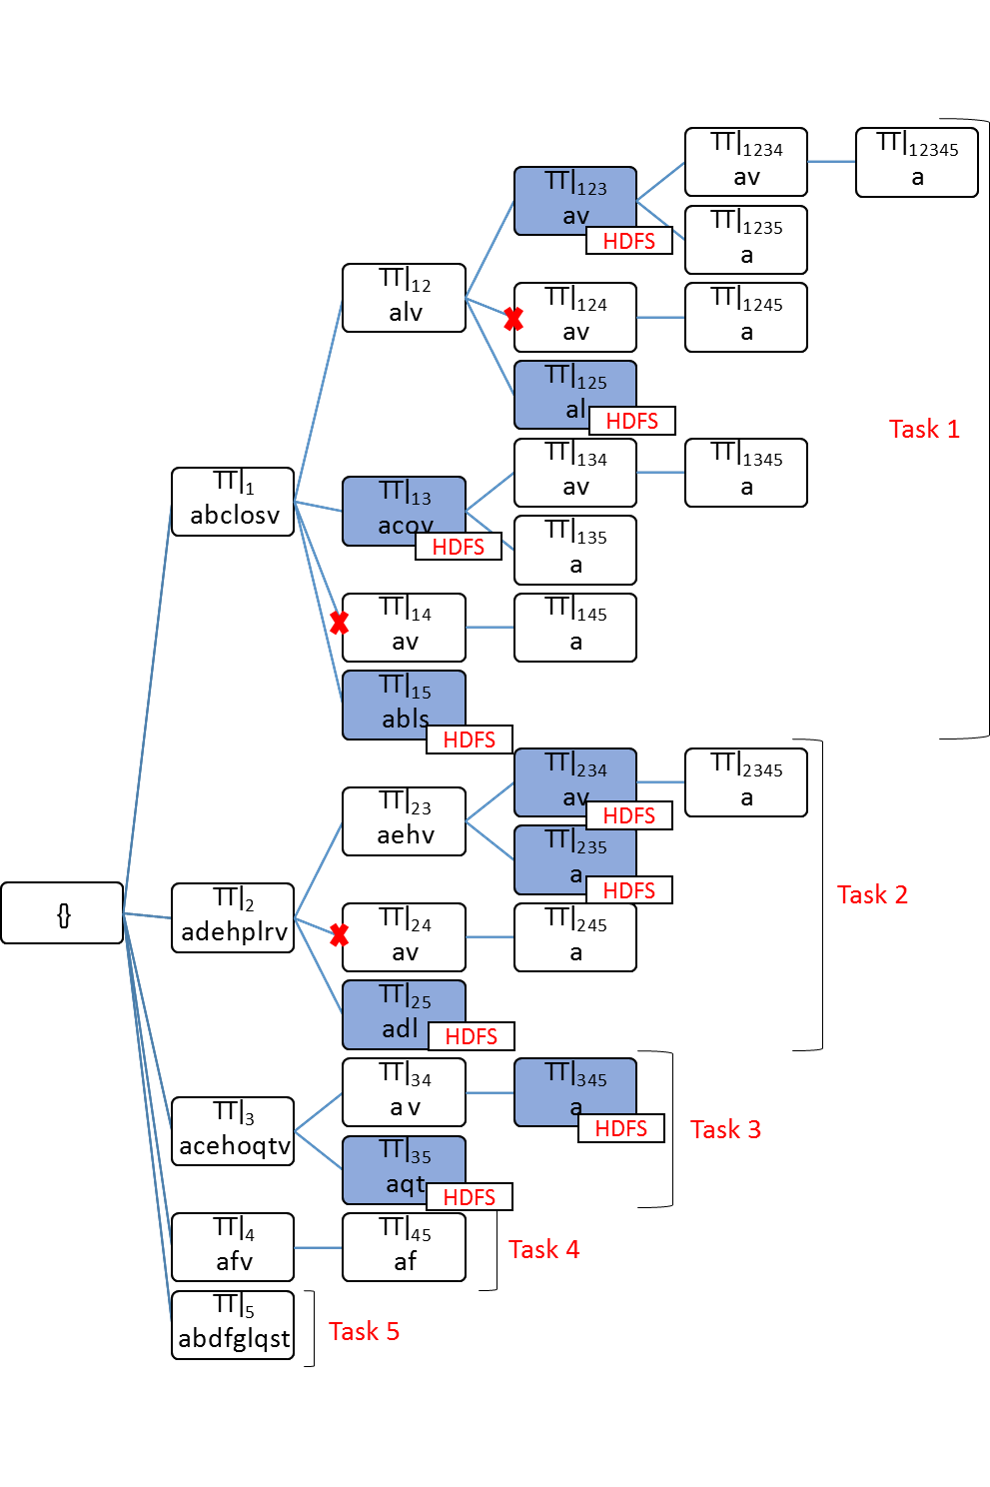
\includegraphics[width=4in]{chapters/pampa/running_example3_d_A.png}
% where an .eps filename suffix will be assumed under latex,
% and a .pdf suffix will be assumed for pdflatex; or what has been declared
% via \DeclareGraphicsExtensions.
\caption{Execution of PaMPa-HD on the running example dataset.
For the sake of clarity, pruning rules 1 and 2 are not
applied. The dark nodes represent the nodes that have been written to HDFS in
order to apply the synchronization job.}

%The red crosses on nodes represent that the nodes have been removed by the
%local pruning, e.g.,
%the one on node \{2 4\} represents the pruning of node \{2 4\}.

\label{running_3}
\end{figure}

\begin{figure}[!t]
%\centering
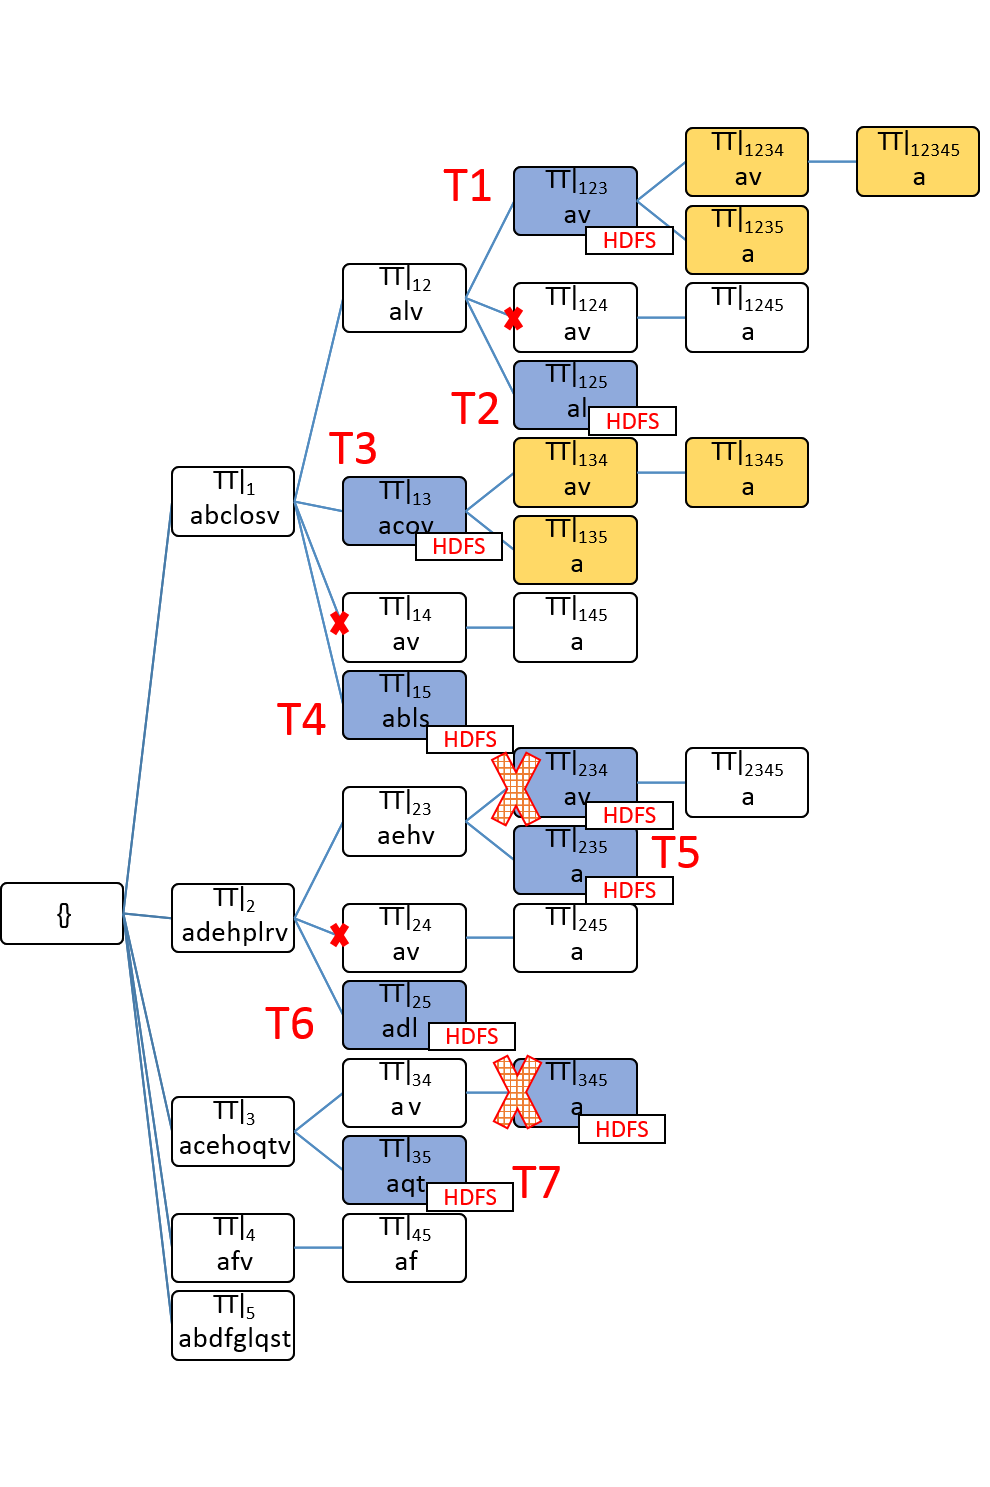
\includegraphics[width=4in]{chapters/pampa/running_example3_d_B_quadretti.png}
% where an .eps filename suffix will be assumed under latex,
% and a .pdf suffix will be assumed for pdflatex; or what has been declared
% via \DeclareGraphicsExtensions.
\caption{Execution of PaMPa-HD on the running example dataset.
For the sake of clarity, pruning rules 1 and 2 are not
applied. The big checked crosses on nodes represent the nodes which have been
removed by the synchronization job, e.g.,
the one on node \{2 3 4\} represents the pruning of node \{2 3 4\}.}
\label{running_3b}
\end{figure}

%Each worker node does not
%run Carpenter to the end but stops and writes intermediate results to the disk.
%After that, the redundancy is deleted with a synchronization job and Carpenter
%starts again from the filtered tables, handled in parallel by different tasks.





\subsection{Implementation details}
\label{MapReduce Carpenter}
PaMPa-HD implementation uses the Hadoop MapReduce framework.
The algorithm consists of three MapReduce jobs as shown in PaMPa-HD pseudocode
(Algorithm~\ref{alg1}).

\begin{algorithm}[t]
\scriptsize
\centering
\caption{PaMPa-HD at a glance}
 \label{alg1}
%\fbox{\parbox{0.9\linewidth}{
 \begin{algorithmic}[1]
 \Procedure{PaMPa-HD}{$minsup;$ $initial$ $TT$}
\State Job 1 Mapper: process each row of TT \par
and send it to reducers, using as key values \par the tids of the tidlists

\State Job 1 Reducer: aggregate $TT|_{x}$ and run \par local Carpenter until
expansion threshold is \par reached  or memory is not enough
\State Job 2 Mapper: process all the closed itemset \par or transposed
 tables from the previous job \par and send them to reducers
\State Job 2 Reducer: for each itemset belonging \par to a table or a frequent
closed, keep \par the eldest in  a Depth First fashion
\State Job 3 Mapper: process each closed itemset \par and $TT|_{x}$ from  the
previous job. \par For the transposed tables run
local Carpenter \par until  expansion  threshold is reached
\State Job 3 Reducer: for each itemset belonging \par to a table or a frequent
closed, keep \par the eldest in  a Depth First fashion
\State Repeat Job 3 until there are no more \par conditional tables

 \EndProcedure
 \end{algorithmic}
%}
%}
\end{algorithm}

% \caption{PaMPa-HD pseudo code}


The Job 1, whose pseudocode is reported in Algorithm~\ref{job1},
 is developed to distribute the input dataset to the independent
tasks,
which will run a local and partial version of the Carpenter algorithm. 
The second job performs the synchronization of the partial results and 
exploits the pruning rules. At the end, the last job interleaves the Carpenter
execution with the synchronization phase.\\


\textbf{Job 1} (Algorithm~\ref{job1}). Each mapper is fed
with a transaction of the input dataset, which is supposed to be in a vertical
representation, together with the minsup parameter. As detailed in
Algorithm~\ref{job1}, each transaction is in the form $item,tidlist$.
For each transaction, the mapper performs
the following steps. For each tid $t_{i}$ of the input tidlist, given
$TL_{greater}$ the set of tids $(t_{i+1},t_{i+2},...,t_{n})$ greater than the
considered tid $t_{i}$ (lines 2-7 in Algorithm~\ref{job1}).
\begin{itemize}
%\item If $|TL_{greater}|+1 <= minsup$, output a key-value pair
%\textless key= $t_{i}$; value= $TL_{greater}$, item\textgreater,
%then analyze $t_{i+1}$ of the tidlist.
\item If $|TL_{greater}| >= minsup$, output a key-value pair \textless key=
$t_{i}$; value= $TL_{greater}$, item\textgreater, then analyze $t_{i+1}$ of the
tidlist.

 \item Else discard the tidlist.
\end {itemize}
 For instance, if the input transaction is the tidlist of item b (b, 1 2 3) and
 minsup is 1, the mapper will output three pairs:  \textless key=1; value=2 3,
 b\textgreater,  \textless  key=2; value=3, b\textgreater,  \textless  key=3;
 value=b\textgreater .\\
 After the map phase, the MapReduce shuffle and sort phase aggregates the
 \textless key,value\textgreater pairs and delivers to reducers the nodes of the
 first level of the tree, which represent the transposed tables projected on a
 single tid (lines 10-13 in Algorithm~\ref{job1}). The tables in Figure~\ref{examplejob1} illustrate the processing of
a row of the initial Transposed  representation of $D$.
Given that each key matches a single transposed table $TT_{X}$, each
reducer builds the transposed tables with the tidlists contained in the
``value'' fields.


From this table, a local Carpenter routine is run (line 14 in Algorithm~\ref{job1}). Carpenter recursively processes a transposed
table expanding it in a depth-first manner (see Section~\ref{Carpenter algorithm} for further details). 
However, the local Carpenter routine stops when the number of processed transposed tables is over the given maximum
expansion threshold. This allows periodically performing the synchronization among the parallel tasks and
hence enforcing pruning rule~3.
All the intermediate results of the local invocation of the Carpenter routine are written to HDFS (lines 15-17 in Algorithm~\ref{job1}).
%\textbf{Fabio: Ho un po' uniformato questo recap ma nn so se eliminarlo}
%The Reducer routine of Job 1, can be resumed in these phases:
% \begin{enumerate}
% \item The transposed table is composed using the tidlists from each key-value
% and a local Carpenter job is run (lines 10-14 in Algorithm~\ref{job1})
% \item For each table a local Carpenter is run. At each recursion of the Carpenter main routine, a counter is incremented: \begin{enumerate}
%\item if the counter is below the threshold, another Carpenter recursion is
%scheduled (lines 14 in Algorithm~\ref{job1})
%\item else, Carpenter main routine is not invoked anymore but all the
% intermediate results are written to HDFS (lines 15-17 in Algorithm~\ref{job1})
%\end{enumerate}
%\end{enumerate}

During the local Carpenter process, the found closed itemsets and the explored
branches are
 stored in memory in order to apply a local pruning. The closed itemsets are
emitted as output at the end of the task, together with the tidlist of the node
of the tree in
which they have been found (lines 18-20 in Algorithm~\ref{job1}). This information is required by the synchronization
phase in order to establish which element is the eldest in a depth first
exploration, i.e., which element is visited  first in a depth first
exploration (e.g. the node associated with tidlist \{1, 2,
3, 5\} is eldest than the node associated with tidlist \{2, 3, 4\} in a depth-first exploration order).\\

\begin{algorithm}[H]
\scriptsize
\centering

\caption{Dataset distribution and local and partial Carpenter execution (Job 1)}
 \label{job1}
 \begin{algorithmic}[1]
  \Procedure{Mapper}{$minsup; item_{i};tidlist$ $TL$}
\For{$j =  0$  to $|(TL)|-1$}
 \par tidlist $TL_{greater}$ : set of tids greater than \par the considered tid
$t_{j}$.
% %\State $Output(  \textless itemset;tidlist$ $+$ $table$ $content$  \Statex
% \pushcode[0] $/support) \textgreater) $
% \If{ $|TL_{greater}|+1 \ge minsup$}
\If{ $|TL_{greater}| \ge minsup$}
 \State output \textless key= $t_{j}$; value= $TL_{greater}$, item\textgreater
 \Else $ $ Break
 \EndIf
\EndFor
\EndProcedure
%\Procedure{Reducer}{$key= tid$ $X, value=list$ $of$ $tidlists$ $TL[$ $]$}
\Procedure{Reducer}{$key= tid$ $X, value=tidlists$ $TL[$ $]$}
\State Create new transposed table $ TT|_{X} $
\For{\textbf{each} tidlist $TL_{i}$ of $TL[$ $]$}
%\State  add $TL_{i}$ to $ TT|_{row_{i}} $ (populate the transposed table)
\State  add $TL_{i}$ to $ TT|_{X} $ (populate the transposed table)
\EndFor

\State Run $Carpenter (minsup;  TT|_{X}; max\_exp)$ 

%\State\hspace{\algorithmicindent}Output (Frequent Closed itemsets)
%\State\hspace{\algorithmicindent} Output (Transposed tables)
%\State\hspace{\algorithmicindent}$Output( \textless frequent$
%$closed$ $itemsets\textgreater )$
%\State\hspace{\algorithmicindent}$Output \textless itemset;$ $tidlist+Transposed
%Table$ $I$ $rows  \textgreater$
\For{\textbf{each} transposed table I found but not processed}
\State $Output \textless itemset;$ $tidlist+Transposed
Table$ $I$ $rows  \textgreater$
\EndFor
\For{\textbf{each} frequent closed itemset found}
\State $Output(  \textless itemset;tidlist+support \textgreater) $
\EndFor
 \EndProcedure
 \end{algorithmic}
\end{algorithm}

\begin{figure}[]
%\renewcommand{\arraystretch}{1.3}
%\centerline
{\subfloat[Transposed representation of $\mathcal{D}$: tidlist of item $a$]{
\label{TTexampledataset_}
\begin{tabular}{|l|l|}
\hline

	item & tidlist \\ \hline
	a & 1,2,3,4,5 \\ \hline
\end{tabular}}}%
\hfil
{\subfloat[Emitted key-value entries from the example row in Table
\ref{TTexampledataset} ]{
\label{key-value}
\begin{tabular}{|l|l|}
\hline

%\multicolumn{2}{|c|}{$TT|_{\{2,3\}}$}\\
%\hline
%\hline
key & value\\ \hline
1 & 2,3,4,5 \textbar  a \\
 \hline
2 & 3,4,5 \textbar  a \\ \hline
3 & 4,5 \textbar  a\\ \hline
4 &5 \textbar  a \\ \hline
5 & - \textbar  a \\ \hline
\end{tabular}}}%
\hfil
{\subfloat[key-value entries for key $3$]{
\label{key-value 3}
\begin{tabular}{|l|l|}
\hline
%\multicolumn{2}{|c|}{$TT|_{\{2,3\}}$}\\
%\hline
%\hline
key & value\\ \hline
3 & 4,5 \textbar a \\ \hline
3 & - \textbar c \\ \hline
3 & - \textbar e \\ \hline
3 & - \textbar h \\ \hline
3 & - \textbar o \\ \hline
3 & 5 \textbar  q \\ \hline
3 & 5 \textbar  t \\ \hline
3 & 4 \textbar  v \\ \hline
\end{tabular}}}%
\hfil
{\subfloat[$TT|_{\{3\}}$: composed with the received values]{
\label{composed_tt}
\begin{tabular}{|l|l|}
\hline
\multicolumn{2}{|c|}{$TT|_{\{3\}}$}\\
\hline
\hline
item & tidlist \\ \hline
a &4,5 \\ \hline
c & - \\ \hline
e & -\\ \hline
h & -\\ \hline
o & -\\ \hline
q & 5\\ \hline
t & 5\\ \hline
%t & 5\\ \hline
v &4 \\ \hline
\end{tabular}}}%
\caption{Job 1 applied to the running example dataset ($minsup=1$): local Carpenter algorithm
is run from the Transposed Table \ref{composed_tt}. }
\label{examplejob1}
\end{figure}



\textbf{Job 2} (Algorithm~\ref{job2}). The synchronization phase is a straightforward
MapReduce job in which mappers input is the output of the previous job: it is
 composed of the closed frequent itemsets found in the previous Carpenter tasks
 and intermediate transposed tables that still have to be expanded. The itemsets
 are associated to their minsup and the tidlist related to the node of the tree
 in which they have been found; the transposed tables are associated to the
table content,
 the corresponding itemset and the table tidlist. 
\begin{itemize}
\item For each table, the mappers output a pair of the form
\textless key=itemset; value=tidlist,table\_rows\textgreater  (lines 2 - 5 of Algorithm~\ref{job2}); 
\item for each itemset, the mappers output a pair in the form \textless
key=itemset; value=tidlist,minsup\textgreater (lines 6 - 11 of Algorithm~\ref{job2}).
\end{itemize}
 The shuffle and sort phase
 delivers to the reducers the pairs aggregated by keys. The reducers, which
match the buckets introduced in Section~\ref{Distributed implementation
outline}, compare the
 entries and emit, for the same key or itemset, only the oldest version in a
 depth first exploration (lines 15 - 21 of Algorithm~\ref{job2}). For instance, referring to our running example in
Figure~\ref{running_3b}, in the reducer related to the itemset $av$ are collected the
entries related to the nodes $T_{1 2 3}$ and $T_{2 3 4}$. Since the tidlist $1 2
3$ is previous than $2 3 4$ in a depth-first exploration order, the reducer
keeps and emits only the entry related to the node $T_{1 2 3}$.
 With this design, the redundant tables that can be obtained due to the independent nature of the Carpenter tasks, which can explore nodes related to the same itemsets, are discarded. This pruning is very
similar to the one
 performed in centralized memory at the cost of a very MapReduce-like job (similar to a \textit{WordCount} application).\\


\textbf{Job 3} (Algorithm~\ref{job3}). This is a mixture of the two previous
jobs. In the Map phase all the remaining tables
are expandend by a local Carpenter routine. The Reduce phase, instead, applies
the same kind of synchronization that is run in the synchronization job. The job
has two types of input: transposed tables and frequent closed itemsets. The
former are processed respecting a depth-first sorting and expanded until it is
reached the maximum expansion threshold (line 5 of Algorithm~\ref{job3}). From that moment, the tables are not
expanded but sent to the reducers (lines 6 - 8 of Algorithm~\ref{job3}). Please note that the tree exploration
processing the initial transposed tables in a depth-first order is the same
to a centralized architecture, enhancing the impact of pruning rule 3 (which strongly relies on this exploration manner).
The latter (i.e. the frequent closed itemsets of the previous PaMPa-HD job) are
processed in the following way. If in memory there is already an oldest
depth-first entry of the same itemset, the closed itemset is discarded. If there
is not, it is saved into memory  and used to improve the local pruning
effectiveness (lines 2 - 3). At the end of the task, all the frequent closed itemsets found are sent to
the reducers, where the redundant elements are pruned.
This job is iterated until all the transposed tables have been processed.





Thanks to the introduction of a global synchronization phase (Job 2 and
Job 3 in Algorithms 3 and 4),
the proposed PaMPa-HD approach is able to apply pruning rule 3
and handle high-dimensional datasets,
otherwise not manageable due to memory issues.



\begin{algorithm}[H]
\centering
\scriptsize
\caption{Synchronization Phase and exploitation of the pruning rule 3 (Job 2)}
  \label{job2}
 \begin{algorithmic}[1]
  \Procedure{Mapper}{$Frequent$ $Closed$ $itemset;$\par $Transposed$ $table$}
\If {Input $I$ is a table}
\State $itemset\gets ExtractItemset(I)$
\State $tidlist\gets ExtractTidlist(I)$
\State $Output(  \textless itemset;$ $tidlist+table$ $I$ $rows  \textgreater) $
\Else $ $  (i.e. input $I$ is a frequent closed Itemset)
\State $itemset\gets ExtractItemset(I)$
\State $tidlist\gets ExtractTidlist(I)$
\State $support\gets ExtractSupport(I)$
\State $Output(  \textless itemset;tidlist+support \textgreater) $
\EndIf

\EndProcedure
\Procedure{Reducer}{$key=itemset;$\par$value=itemsets$ $\&$ $tables$ $T[$ $]$}
\State $oldest\gets null$
\For{\textbf{each} itemset or table $T$ of  $T[$ $]$}
\State $tidlist\gets ExtractTidlist(T)$
%\If { $tidlist$ previous of $oldest$ in a DFS}
\If { $tidlist$ previous of $oldest$ in a Depth-First Search}
 \State $oldest\gets T$
\EndIf
\EndFor
\State $Output(\textless itemset+oldest\textgreater )$
%% \pushcode[0] $/support) \textgreater) $
% %
 \EndProcedure
 \end{algorithmic}
\end{algorithm}

\begin{algorithm}[H]
\scriptsize
\centering
\caption{Interleaving of the Carpenter execution and synchronization phase (Job 3)}
 \label{job3}
 \begin{algorithmic}[1]
  \Procedure{Mapper}{$Frequent$ $Closed$ $itemset; Transposed$ $table$}
\If {Input $I$ is a frequent closed itemset}
\State save $I$ to local memory

\Else $ $ (i.e. input $I$ is a Transposed Table)
%\State $itemset\gets ExtractItemset(I)$

\State Run $Carpenter (minsup;  TT|_{X};max\_exp)$

\For{\textbf{each} transposed table I found but not processed}
\State $Output \textless itemset;$ $tidlist+Transposed
Table$ $I$ $rows  \textgreater$
\EndFor


%\State\hspace{\algorithmicindent} $Output(  \textless itemset;tidlist+support \textgreater) $
\EndIf
\For{\textbf{each} frequent closed itemset found}
\State $Output(  \textless itemset;tidlist+support \textgreater) $
\EndFor
\EndProcedure
\Procedure{Reducer}{$key=itemset;$\par$value=itemsets$ $\&$ $tables$ $T[$ $]$}
\State $oldest\gets null$
\For{\textbf{each} itemset or table $T$ of  $T[$ $]$}
\State $tidlist\gets ExtractTidlist(T)$
%\If { $tidlist$ previous of $oldest$ in a DFS}
\If { $tidlist$ previous of $oldest$ in a Depth-First Search}
 \State $oldest\gets T$
\EndIf
\EndFor
\State $Output(\textless itemset+oldest\textgreater )$
%% \pushcode[0] $/support) \textgreater) $
% %
 \EndProcedure
 \end{algorithmic}
\end{algorithm}


%%%%%%%%%%%%% Fine sezione algoritmo
%
%\section{Expansion Threshold tuning}
%\label{threshold}
%Before the comparison with the state of the art distributed algorithms in Section~\ref{Experiments}, we performed a set of experiments to measure the performance impact of the maximum expansion threshold, evaluating the quality of a set of proposed strategies. This set of experiments, together with the ones in Section~\ref{Experiments}, are performed on two real life datasets.
The first real dataset is the \textbf{Kent Ridge Breast Cancer}~\cite{breast_cancer_dataset}, which contains gene expression data.
It is characterized by 97 rows that represent patient samples, and
24,482 attributes related to genes. The attributes are numeric (integers, floating point).
Data have been discretized with an equal depth partitioning
using 20 buckets (similarly to \cite{Zaki_Carpenter}).
The second real dataset is the \textbf{PEMS-SF} dataset~\cite{breast_cancer_dataset}, 
which describes the occupancy rate of different car lanes of San Francisco bay area freeways.
Each transaction represents the daily traffic rate of 963 lanes, sampled every 10 minutes.
It is characterized of 440 rows (in some experiments we have utilized only the first 100) and 138672 attributes (6 x 24 x 963), and it has been discretized in
equi-width bins of 0.002.
Because of their distribution and their discretizazion process, the Breast Cancer dataset is more sparse (low correlation among the dataset transactions) than the PEMS-SF dataset. 
The other two datasets were synthetically generated and tuned to simulate
use cases characterized by extremely high-dimensional data,
i.e., with massive numbers of features.
Both datasets consists of 30 transactions.
Dataset~\#1 has 1,000,000 different items
and an average transaction length of 500,000 items,
while
Dataset~\#2 is 10 times larger, with 10,000,000 different items
and an average transaction length of 5,000,000 items
(see Table~\ref{datasets}).
The discretized version of the real dataset and the synthetic dataset generator
are publicly available at http://dbdmg.polito.it/PaMPa-HD/. \textbf{TO DO: aggiungere versione finale discretized pemsf}



\begin{table}[h!]
\begin{center}
\caption{Datasets}
\label{datasets}
\begin{tabular}{|c|c|c|c|}
\hline
	Dataset & Number of  & Number of & Average number  \\
	 & transactions &different items & of items  \\ 
	  &  & &  per trasanaction  \\ \hline
	Kent Ridge Breast    & 97 & 489,640    & 24,492 \\
     CancerDataset      &    &            &  \\ \hline
PEMS-SF    & 440& 5,454,414     & 138,672 \\
     Dataset      & (100 rows version)   &   (3,946,646)       &  \\ \hline
	Synthetic Dataset \#1 & 30 & 1,000,000  & 500,000\\ \hline
	Synthetic Dataset \#2 & 30 & 10,000,000 & 5,000,000\\ \hline
\end{tabular}
\end{center}
\end{table}


PaMPa-HD is implemented in Java 1.7.0\_60 using the Hadoop MR API.
Experiments were performed on a cluster of 5 nodes running Cloudera
Distribution of Apache Hadoop (CDH5.3.1).
Each cluster node is a 2.67 GHz six-core Intel(R) Xeon(R) X5650 machine
with 32 Gbyte of main memory
running Ubuntu 12.04 server with the 3.5.0-23-generic kernel.


\subsection{Impact of the maximum expansion threshold}\label{exp_fisso}
As already mentioned in Section~\ref{Distributed implementation outline}, the maximum expansion threshold
($max\_exp$) parameter indicates the maximum number of nodes 
to be explored before a preemptive stop of each distributed sub-process is forced.
This parameter strongly affects the enumeration tree exploration,
forcing each parallel task to stop before completing the visit of its sub-tree 
and write partial results on HDFS. 
This approach allows the synchronization job to globally apply 
pruning rule 3 and reduce the search space.
Low values of $max\_exp$ threshold decrease the risks of memory issue, 
because the global problem is split into simpler and less memory-demanding
sub-problems, and facilitate the application of pruning rule 3, 
hence a smaller subspace is searched.
However, higher values allow a more efficient execution,
by limiting the start and stop of distributed tasks
(similarly to the context switch penalty), and the synchronization overheads.

In order to assess the impact of the expansion threshold parameter, we performed two set of experiments. In the first one we have performed the mining on the PEMS-SF (100 transactions) dataset with a Minsup 50, by varying $max\_exp$ from 10 to 100,000,000.  The minsup value was empirically selected in order to let the mining problem being deep enough to show up different performances. 
In Figure~\ref{pems_fixed} are shown the results in terms of execution time and number of iterations 
(i.e., the number of jobs).

It is clear how the $max\_exp$ parameter can influence the performance, with wall-clock times that can be doubled with different configurations. The best performance in terms of execution time is achieved with a maximum
expansion threshold equal to 10,000 nodes. With lower values, the execution times are slightly longer, while there is an evident performance degradation with higher $max\_exp$ values. 
This result highlights the importance of the synchronization phase.
Increasing the $max\_exp$ parameter makes the number of iterations decreasing,
but more useless tree branches are explored,
because pruning rule 3 is globally applied less frequently.
Lower values of  $max\_exp$, instead, raising the number of iterations
, introduce a slight performance
degradation caused by iterations overheads.
%With very high values of  $max\_exp$, the running time and the number of
%iterations are stable because the bottleneck becomes the free available
%memory, and the synchronization job is
%automatically applied, independently of the value of  $max\_exp$.

\begin{figure}[!t]
\includegraphics[width=5in]{immagini_extension/pems_fixed.png}
\caption{Execution time and number of iterations for different $max\_exp$ values on PEMS-SF dataset with $minsup$=50.
}
\label{breast_fixed}
\end{figure}

\begin{figure}[!t]
\includegraphics[width=5in]{immagini_extension/breast_fixed.png}
\caption{Execution time and number of iterations for different $max\_exp$ values on Breast Cancer dataset with $minsup$=6.
}
\label{pems_fixed}
\end{figure}

The same experiment is repeated with the Breast Cancer dataset and a minsup value of 6. As shown in Figure~\ref{breast_fixed}, this time the best performances are achieved with $max\_exp$ equal to 100,000. In this case, indeed, cannot be noted big differences with the higher values. Instead, the performances strongly decreases with lower values of $max\_exp$ parameter.



\textbf{+ menzione a load balancing}.







The $max\_exp$ choice has a non-negligible impact on the performances of the algorithm. As demonstrated by the curves in Figures~\ref{pems_fixed} and~\ref{breast_fixed}, it is very dependent on the use case and distribution of the data. In order to simplify the parameter configuration for the user and, above all, increase the performance of the algorithm, we have implemented some tuning strategies related to $max\_exp$, prensented in the next subsection.
%
%This set of experiments has been performed on the Breast cancer dataset
%with Minsup 5, by varying $max\_exp$ from 100 to 100,000,000. This minsup value allowed to notice different
%wall-clock time for each expansion threshold value.
%Figure~\ref{exp_1} shows the results in terms of execution time and number of iterations 
%(i.e., the number of jobs).
%The best performance in terms of execution time is achieved with a maximum
%expansion threshold equal to 10,000 nodes.
%With higher values, the number of iterations decreases,
%but more useless tree branches are explored,
%because pruning rule 3 is globally applied less frequently.
%Lower values of  $max\_exp$, instead, introduce a performance
%degradation caused by the higher number of iterations
%and the synchronization phase overheads.
%With very high values of  $max\_exp$, the running time and the number of
%iterations are stable because the bottleneck becomes the free available
%memory, and the synchronization job is
%automatically applied, independently of the value of  $max\_exp$.
%The tuning of $max\_exp$ is strictly related to the data distribution:
%in general, the easier the mining task, the fewer the benefits of having 
%many iterations.
%
%The value of $max\_exp$ impacts also the load balancing 
%of the distributed computation among different nodes.
%With low values of $max\_exp$, each task explores a
%smaller enumeration sub-tree, decreasing the size difference
%among the sub-trees analyzed by different tasks,
%thus improving the load balancing.
%Table~\ref{load balance} reports the minimum and the maximum execution time of
%the mining tasks executed in parallel for two extreme values of $max\_exp$. 
%The load balance is better for the lowest value of $max\_exp$.
%\textbf{tutto vecchio fin qui}
%
%
%\begin{figure}[!t]
%\includegraphics[width=3.5in]{grafo_exp2.png}
%\caption{Execution time and number of iterations for different $max\_exp$ values on Breast Cancer dataset with $minsup$=5.
%}
%\label{exp_1}
%\end{figure}
%
%
%\begin{table}
%\begin{center}
%\caption{Load Balancing}
%\label{load balance}
%\begin{tabular}{ |c| c | c| }
%\hline
%							    &
%\multicolumn{2}{|c|}{Task execution time}          \\ \hline
%	Maximum expansion threshold &   Min          & Max            \\ \hline
%	100,000,000                 &    4s                      & 1h 54m 33s
%  \\ \hline
%100,000                 &    4s                      & 1h 2m 32s
%  \\ \hline
%	10000                         &    4s                      &        23m 50s
%\\ \hline
%100                         &    4s                      &        53s
% \\ \hline
%\end{tabular}
%\end{center}
%\end{table}


\subsection{Proposed strategies}\label{exp_strategies}
This section introduces some heuristic strategies related to the $max\_exp$ parameter. 
The aim of this experiment is to identify an heuristic technique which is able to deliver good performances without the need by the user to tune up the the $max\_exp$ parameter.
Before the introduction of the techniques, let us motivate the reasons behind their design.
Because of the enumeration tree architecture, the first tables of the tree are the most populated. Each node, in fact, is generated from its parent node as a projection of the parent transposed table on a tid. 
In addition, the first nodes are, in the average, the ones generating more sub-branches. By construction, their transposed table tidlists are, by definition, longer than the ones of their children nodes. This increases the probability that the table could be projected on a tid.
For these reasons, the tables of the initial mining phase are the most heavy to be processed.
On the other hand, the number of nodes to process by each local Carpenter iteration tends to increase with the number of iterations. Still, this factor is mitigated by (i) the decreasing size of the tables and (ii) the eventual end of some branches expansion (i.e. when there are not more tids in the node transposed table).
These reasons, motivated us to introduce some strategies that assumes a maximum expansion threshold that is increased with the number of iterations. These strategy start with very low values in very initial iterations  (i.e. when the nodes are more heavy to be processed) and increase $max\_exp$ during the mining phases.

%Finally, in all the experiments \textbf{citare quelli di prima}, we have notices some very short execution times (less than a minute) in the last mining iterations. This surely increases the impact of MapReduce job handling overhead on the global performances.
%All these things, motivated us to introduce some strategies that assumes a maximum expansion threshold that is increased with the number of iterations.
%All these things, together with very short last iterations (with an increasing MapReduce job overhead), motivated us to test some strategies that assumes a maximum expansion threshold that is increased with the iterations.

The strategy \#1 is straightforward: the $max\_exp$ is increased with a factor of $X$ at each iteration. For instance, if the $max\_exp$ is set to 10, and $X$ is set to 100 at the second iteration it is raised to 1000 and so on. 

Alternatively, we wanted to achieve a balanced growth of the $max\_exp$ parameter. We want to balance the load of the iterations, but, on the other hand, we want to avoid an overgrowth of the parameter and, therefore, of the execution times of the last iterations. As already said, in fact, increasing the $max\_exp$ parameter decreases the impact of the synchronization job pruning.
In order to monintor the growth, we introduced a set of techniques based on the execution times and a strategy which monitors the impact of the synchronization jobs.
%In order to monitor this growth, we firstly thought about an index measuring the effectiveness of the pruning in terms of closed or tables pruned in the synchronization job. However, the effectiveness of the pruning cannot be easily interpreted. An increasing pruning effect means that there are a lot of tables that are generated uselessly. However, an increasing pruning effect is also normal since the number of nodes that are processed continues to increase. \textbf{inserire degli esperimenti in cui faccio vedere che usare il pruning effect riduce le performance}.
In strategies \#2 and \#3, we took into exam the execution time of the iterations.
Spefically, strategy \#2 consists in increasing, at each iteration, the $max\_exp$ parameter with a factor of  $X^{T_{old} / T_{new}}$, given $T_{new}$ and  $T_{old}$ the execution time of the previous two jobs. The motivation is to balance the growth of the parameter in order to achieve a stable execution times among the iterations.  
Strategy \#3, instead, is inspired by the congestion control of TCP/IP (a data transmission protocol used by many Internet applications \cite{}). Precisely, the $max\_exp$ is handled like the congestion window size (i.e. the number of packets that are sent without congestion issues).
This strategy, called ``Slow Start'', assumes two types of growing of the window size: an exponential one and a linear one. In the first phase, the window size is increased exponentially until it reaches a threshold (``ssthresh'', which is calculated empirically from RTT and other values). From that moment, the growth of the window becomes linear, until a data loss occurs.
In our case, we are not interested we just inherit the two growth factors. Therefore, our ``slow start'' strategy consists in increasing the $max\_exp$ of a factor of $X$ until the last iteration reaches an execution time greater than a given threshold. After that, the growth is more stable, increasing the parameter of a factor of 10 (for this reason $X$>10).
We have fixed the threshold to the execution time of the first two jobs (Job 1 and Job 2). These jobs, for the architecture of our algorithm, consists of the very first Carpenter iteration. They are quite different than the others since the first Mapper phase has to build the initial projected transposed tables (first level of the tree) from the input file. 
We have selected the execution time of the first iteration since it is consistent with our initial aim,
that is to normalize the execution times of the last iterations which are often shorter than the first ones.

The last strategy, \#4, is based on the effectiveness of the pruning in terms of closed or tables pruned in the synchronization job. Indeed, the measure of the relative number of tables that are pruned cannot be easily interpreted. An increasing pruning percentage means that there are a lot of tables that are generated uselessly. However, an increasing trend is also normal, since the number of nodes that are processed continues to increases. Given that our intuition is to rise the  $max\_exp$ among the iterations, in strategy \#4, we increase the $max\_exp$ parameter with a factor $X^{Pr_{old} / Pr_{new}}$, given $Pr_{new}$ and  $Pr_{old}$ the relative number of pruned tables in the previous two jobs. 
%Even if strategy \#4 can be meant as the dual of strategy \#2, with the usage of the pruning ratios instead of the different execution times, we decided not to do the same for strategy \#3. In this case, we could not identify a proper threshold to be used for changing the growth factor of $max\_exp$. In strategy \#3, we have used the first iteration because the initial motivation of this empirical study is to stabilize the execution times. In this case, we don't consider the initial pruning ratio as a valid threshold: it is computed after only few tables and, in the worst case, can be 0.

In our experiment, we have fixed the initial  $max\_exp$ value to 10. This very low value is motivated by the nature of our strategies, which consist of a balanced increasing of the parameter.
We applied the strategies (resumed in Table~\ref{table_strategies}) to the same experiments of Figures~\ref{breast_fixed} and ~\ref{pems_fixed}, in order to compare execution times the ones obtained with the optimum choice of $max\_exp$. 
In oder to assess the impact of the $X$ parameter, we have used values from 10 to 10,000 (except for strategy3 for which we have used values from 100 to 10,000).

The result of the application of the techniques to the PEMS-SF dataset are shown in Figures~\ref{pems_strategy1},~\ref{pems_strategy2},~\ref{pems_strategy3},~\ref{pems_strategy4}, which represent the relative execution time gain with respect to the best execution time obtained with the fixed $max\_exp$ of 10,000. In Figure~\ref{pems_strategy_best} we have grouped the best configuration for each strategy in order to easily compare them.
It is clear how the almost all the strategies improve the performance of the algorithm. Only Strategy3 showed to be slower. Strategy1(1,000), Strategy2(10,000) and Strategy4(1,000) achieve a very similar speedup. 

We have repeated the experiment with Breast Cancer dataset and a minsup value of 6 (Figures~\ref{breast_strategy1},~\ref{breast_strategy2},~\ref{breast_strategy3},~\ref{breast_strategy4}). We have raised $X$ from 10 to 10,000. Only with Strategy2, as shown in Figure~\ref{breast_strategy2}, we have raised it to 100,000 , because the experiments could suggest a decreasing execution times trend, but it was not the case.
As before, the results are grouped in Figure~\ref{breast_strategy_best}.
In this case, all the strategies achieve a positive speedup with respect to the best execution time obtained with a fixed $max\_exp$ parameter. In addition, the same configurations for each strategy demonstrated to be most performant in both the experiments.
The results obtained with the adoption of these strategies are very similar, and the differences are negligible.



\begin{table}
\begin{center}
\caption{Strategies}
\label{table_strategies}
\begin{tabular}{|c|c|}
\hline
Strategy \#1($X$)  & Increasing at each iteration      \\ 
                   & with a factor of $X$               \\ \hline

Strategy \#2($X$)  & Increasing at each iteration with \\
                   & a factor of $X^{T_{old} / T_{new}}$                   \\ \hline

Strategy \#3       & Slow start, with a fast increase                      \\ 
     & factor of   $X$                     \\ \hline
Strategy \#4($X$) & Increasing at each iteration with \\
                   & a factor of $X^{Pr_{old} / Pr_{new}}$                    \\ \hline
            
\end{tabular}
\end{center}
\end{table}

\begin{figure}[!t]
\includegraphics[width=5in]{immagini_extension/pems_strategy1.png}
\caption{Relative gains on Pems-SF dataset with $minsup$=50, Strategy1 and different $X$ values.
}
\label{pems_strategy1}
\end{figure}

\begin{figure}[!t]
\includegraphics[width=5in]{immagini_extension/pems_strategy2.png}
\caption{Relative gains on Pems-SF dataset with $minsup$=50, Strategy2 and different $X$ values.
}
\label{pems_strategy2}
\end{figure}

\begin{figure}[!t]
\includegraphics[width=5in]{immagini_extension/pems_strategy3.png}
\caption{Relative gains on Pems-SF dataset with $minsup$=50, Strategy3 and different $X$ values.
}
\label{pems_strategy3}
\end{figure}

\begin{figure}[!t]
\includegraphics[width=5in]{immagini_extension/pems_strategy4.png}
\caption{Relative gains on Pems-SF dataset with $minsup$=50, Strategy4 and different $X$ values.
}
\label{pems_strategy4}
\end{figure}

\begin{figure}[!t]
\includegraphics[width=5in]{immagini_extension/pems_strategy_best.png}
\caption{Relative gains of the best configuration for each strategy, on Pems-SF dataset with $minsup$=50.
}
\label{pems_strategy_best}
\end{figure}


\begin{figure}[!t]
\includegraphics[width=5in]{immagini_extension/breast_strategy1.png}
\caption{Relative gains on Breast dataset with $minsup$=6, Strategy1 and different $X$ values.
}
\label{breast_strategy1}
\end{figure}

\begin{figure}[!t]
\includegraphics[width=5in]{immagini_extension/breast_strategy2.png}
\caption{Relative gains on Breast Cancer dataset with $minsup$=6, Strategy2 and different $X$ values.
}
\label{breast_strategy2}
\end{figure}

\begin{figure}[!t]
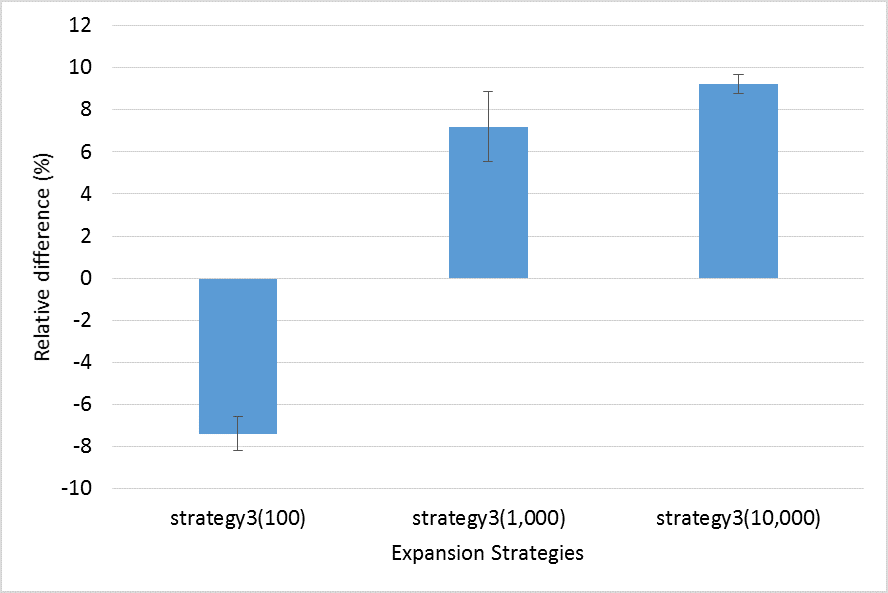
\includegraphics[width=5in]{immagini_extension/breast_strategy3.png}
\caption{Relative gains on Breast Cancer dataset with $minsup$=6, Strategy3 and different $X$ values.
}
\label{breast_strategy3}
\end{figure}

\begin{figure}[!t]
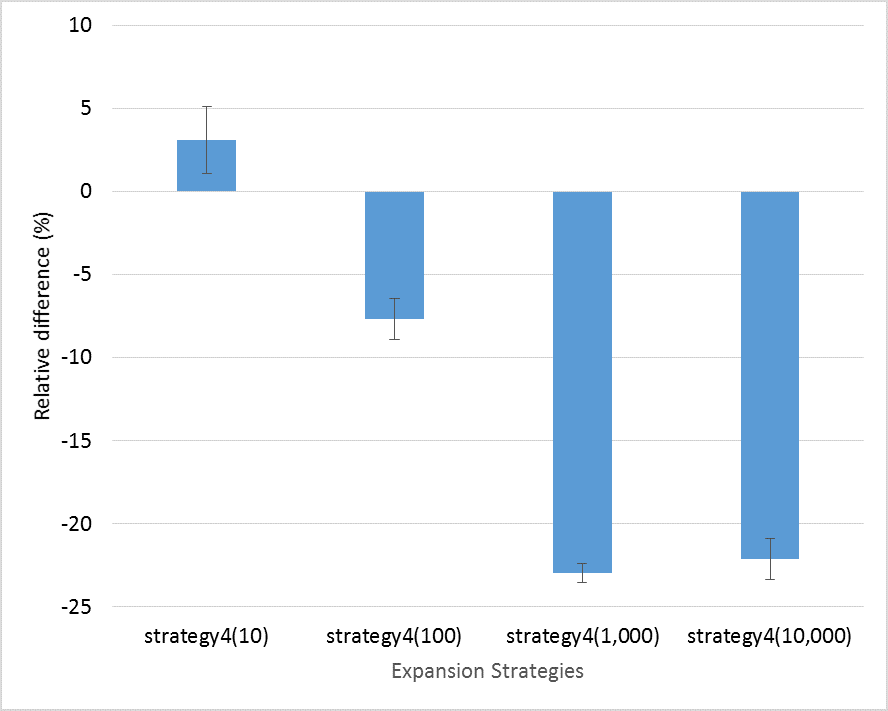
\includegraphics[width=5in]{immagini_extension/breast_strategy4.png}
\caption{Relative gains on Breast Cancer dataset with $minsup$=6, Strategy4 and different $X$ values.
}
\label{breast_strategy4}
\end{figure}

\begin{figure}[!t]
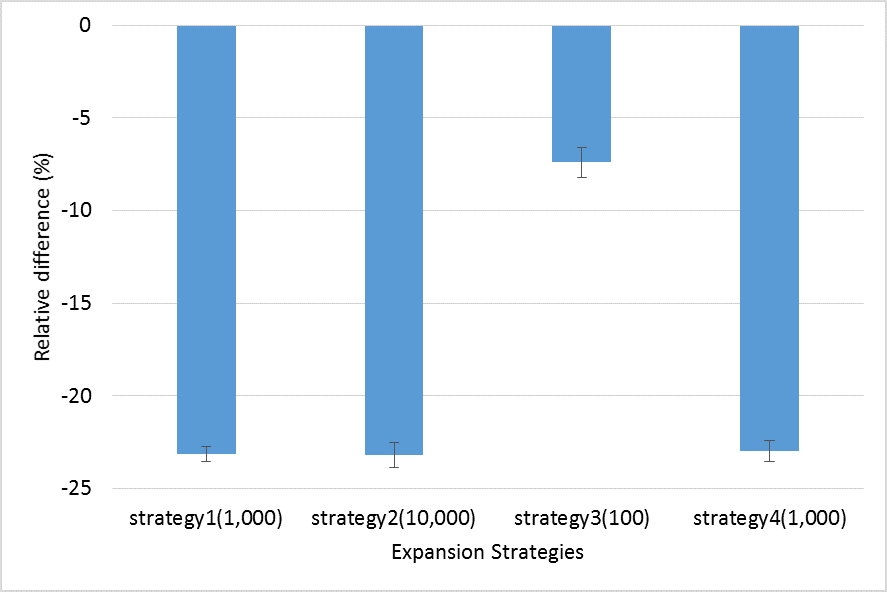
\includegraphics[width=5in]{immagini_extension/breast_strategy_best.png}
\caption{Relative gains of the best configuration for each strategy, on Pems Cancer dataset with $minsup$=6.
}
\label{breast_strategy_best}
\end{figure}




\section{Experiments}
\label{Experiments}
In this section, we present a set of experiments to evaluate the performance of the proposed algorithm. 
Firstly, we asses the impact on performance of the maximum expansion threshold ($max\_exp$ ) parameter (Section~\ref{exp_fisso}). This phase is mandatory in order to tune-up the parameter configuration to compare the proposed approach with the state-of-the-art algorithms. Because the tuning of the parameter is not trivial, 
we discuss and experimentally evaluate some self-tuning
strategies to automatically set the $max\_exp$ parameter and improve the performance (Section~\ref{exp_strategies}). 

Next, we evaluate the speed of the proposed algorithm,
comparing it with the state-of-the-art distributed approaches 
(Section~\ref{running_time}). 
Finally, we experimentally analyze the impact of 
(i) the number of transactions of the input dataset (Section~\ref{number_rows}),
(ii) the number of parallel tasks (Section~\ref{scalability}), and
(iii) the communication costs and load balancing behavior (Section~\ref{communication_cost}).

Experiments have been performed on two real-world datasets.
The first is the PEMS-SF dataset~\cite{uci},
which describes the occupancy rate of different car lanes 
of San Francisco bay area freeways 
(15 months worth of daily data from the California Department of Transportation~\cite{pems}).
Each transaction represents the daily traffic rates of 963 lanes, sampled every 10 minutes.
It is characterized by 440 rows and 138,672 attributes (6 x 24 x 963), 
and it has been discretized in equi-width bins, each representing 0.1\% occupancy rate.

%Since PaMPa-HD is designed to cope with high-dimensional datasets 
%characterized by a small number of transactions, 
%we have used several down-sampled versions (in terms of number of rows) of the datasets 
%to measure the impact of the number of transactions on the performance of the algorithm.
As mentioned, PaMPa-HD design is focused on scaling up in terms of number of attributes, 
being able to cope with high-dimensional datasets. For this reason, we have used a 100-rows version of the PEMS-SF dataset for all the experiments. However, we have used the full dataset and several down-sampled versions (in terms of number of rows) to measure the impact of the number of transactions on the performance of the algorithm (Section~\ref{number_rows}).
%characterized by a small number of transactions, 
%we have used several down-sampled versions (in terms of number of rows) of the datasets 
%to measure the impact of the number of trfactions on the performance of the algorithm.

The second dataset is the Kent Ridge Breast Cancer~\cite{breast_cancer_dataset}, 
which contains gene expression data.
It is characterized by 97 rows that represent patient samples, 
and 24,482 attributes related to genes.
The attributes are numeric (integers and floating point).
Data have been discretized with an equal-depth partitioning
using 20 buckets (similarly to~\cite{Zaki_Carpenter}).
The discretized versions of the real datasets
are publicly available at http://dbdmg.polito.it/PaMPa-HD/.

%Because of their distribution and their discretizazion process, the Breast Cancer dataset is more sparse (low correlation among the dataset transactions) than the PEMS-SF dataset.
%The other two datasets were synthetically generated and tuned to simulate
%use cases characterized by extremely high-dimensional data,
%i.e., with massive numbers of features.
%Both datasets consists of 30 transactions.
%Dataset~\#1 has 1,000,000 different items
%and an average transaction length of 500,000 items,
%while
%Dataset~\#2 is 10 times larger, with 10,000,000 different items
%and an average transaction length of 5,000,000 items
%(see Table~\ref{datasets}).



\begin{table}[h!]
\begin{center}
\caption{Datasets}
\label{datasets}
\begin{tabular}{|c|c|c|c|}
\hline
	Dataset & Number of  & Number of & Number  \\
	 & transactions &different items & of items  \\
	  &  & &  per transaction  \\ \hline \hline

PEMS-SF    & 440& 8,685,087     & 138,672 \\
   %  Dataset      & (100 rows version)   &   (5,748,097)       &  \\ \hline
       Dataset      &  &          &  \\ \hline
     Kent Ridge Breast    & 97 & 489,640    & 24,492 \\
     Cancer Dataset      &    &            &  \\ \hline
%	Synthetic Dataset \#1 & 30 & 1,000,000  & 500,000\\ \hline
%	Synthetic Dataset \#2 & 30 & 10,000,000 & 5,000,000\\ \hline
\end{tabular}
\end{center}
\end{table}


PaMPa-HD is implemented in Java 1.7.0\_60 using the Hadoop MR API.
The experiments were performed on a cluster of 5 nodes running Cloudera
Distribution of Apache Hadoop (CDH5.3.1).
Each cluster node is a 2.67 GHz six-core Intel(R) Xeon(R) X5650 machine
with 32 Gbyte of main memory
running Ubuntu 12.04 server with the 3.5.0-23-generic kernel.


\subsection{Impact of the maximum expansion threshold}\label{exp_fisso}
In this section we analyze the impact of the maximum expansion threshold
($max\_exp$) parameter, which indicates the maximum number of nodes
to be explored before a preemptive stop of each distributed sub-process is forced.
This parameter, as already discussed in Section~\ref{Distributed implementation outline},
strongly affects the enumeration tree exploration,
forcing each parallel task to stop before completing the visit of its sub-tree
and send the partial results to the synchronization phase.
This approach allows the algorithm to globally apply
pruning rule 3 and reduce the search space.
Low values of $max\_exp$ threshold increase the load balancing,
because the global problem is split into simpler and less memory-demanding
sub-problems, and, above all, facilitate the global application of pruning rule 3,
hence a smaller subspace is searched.
However, higher values allow a more efficient execution,
by limiting the start and stop of distributed tasks
(similarly to the context switch penalty) and the synchronization overheads. Above all, higher values enhance the pruning effect of the state centralized memory.
%\textbf{(Considerare per tutti i grafici una possibile inversione di ordine (mettere prima gli esperimenti con dataset Breast Cancer e poi PEMS-SF), causata dalla `'poca'' bellezza degli esperimenti con strategy 1 per pems dataset. }
In order to assess the impact of the expansion threshold parameter, we have performed two sets of experiments. In the first one we perform the mining on the PEMS-SF (100 transactions) dataset with minsup = 10, by varying $max\_exp$ from 100 to 100,000,000.  The minsup value has been empirically selected to highlight the different performance related to different values (trivial mining would be overwhelmed by overhead costs of the MapReduce framework).
In Figure~\ref{pems_fixed} are shown the results in terms of execution time and number of iterations
(i.e., the number of jobs)\footnote{Please note that in all the experiments, for the sake of clarity, the confidence intervals (obtained after a sufficient number of executions and with  complementary level of significance of 95\%) are omitted from the graphs.}.
It is clear how the $max\_exp$ parameter can influence the performance, with wall-clock times that can be doubled with different configurations. The best performance in terms of execution time is achieved with a maximum
expansion threshold equal to 10,000 nodes. With lower values, the execution times are slightly longer, while there is an evident performance degradation with higher $max\_exp$ values.
This result highlights the importance of the synchronization phase.
Increasing the $max\_exp$ parameter makes the number of iterations decreasing,
but more useless tree branches are explored,
because pruning rule 3 is globally applied less frequently.
Lower values of  $max\_exp$, instead, raising the number of iterations, introduce a slight performance
degradation caused by iterations overheads.
%With very high values of  $max\_exp$, the running time and the number of
%iterations are stable because the bottleneck becomes the free available
%memory, and the synchronization job is
%automatically applied, independently of the value of  $max\_exp$.

\begin{figure}[!t]
\includegraphics[width=5in]{chapters/pampa/immagini_extension/pems_fixed.png}
\caption{Execution time and number of iterations for different $max\_exp$ values on PEMS-SF dataset with $minsup$=10.
}
\label{pems_fixed}
\end{figure}

\begin{figure}[!t]
\includegraphics[width=5in]{chapters/pampa/immagini_extension/breast_fixed.png}
\caption{Execution time and number of iterations for different $max\_exp$ values on Breast Cancer dataset with $minsup$=5.
}
\label{breast_fixed}
\end{figure}

The same experiment is repeated with the Breast Cancer dataset and a minsup value of 5. As shown in Figure~\ref{breast_fixed}, even in this case, the best performances are achieved with $max\_exp$ equal to 10,000. In this case, differences are more significant with lower $max\_exp$ values, although with a non-negligible performance degradation with higher values.

The value of $max\_exp$ impacts also the load balancing
of the distributed computation among different nodes.
With low values of $max\_exp$, each task explores a
smaller enumeration sub-tree, decreasing the size difference
among the sub-trees analyzed by different tasks,
thus improving the load balancing.
Table~\ref{load balance breast} reports the minimum and the maximum execution time of
the mining tasks executed in parallel for both the datasets and for two extreme values of $max\_exp$.
The load balance is better for the lowest value of $max\_exp$.



\begin{table}
\begin{center}
\caption{Load Balancing}
\label{load balance breast}
\begin{tabular}{ |c| c | c| c| c| }
\hline
							    &
\multicolumn{2}{|c|}{Task execution time}    & \multicolumn{2}{|c|}{Task execution time}      \\
 & \multicolumn{2}{|c|}{Breast Cancer}    & \multicolumn{2}{|c|}{PEMS-SF}      \\ \hline \hline
	Maximum expansion threshold &   Min          & Max    &   Min          & Max          \\ \hline
	100,000,000                 &    7 m                      & 2h 16m 17s &    44s                      & 2h 20m 28s
  \\ \hline
10                         &    6m 21s                      &        45m 16s  &   6s                      &        2m 24s
 \\ \hline
\end{tabular}
\end{center}
\end{table}





The $max\_exp$ choice has a non-negligible impact on the performances of the algorithm. However, as demonstrated by the curves in Figures~\ref{pems_fixed} and~\ref{breast_fixed}, it is very dependent on the use case and distribution of the data.
In the next subsection we introduce and motivate some tuning strategies related to $max\_exp$.

%
%This set of experiments has been performed on the Breast cancer dataset
%with Minsup 5, by varying $max\_exp$ from 100 to 100,000,000. This minsup value allowed to notice different
%wall-clock time for each expansion threshold value.
%Figure~\ref{exp_1} shows the results in terms of execution time and number of iterations
%(i.e., the number of jobs).
%The best performance in terms of execution time is achieved with a maximum
%expansion threshold equal to 10,000 nodes.
%With higher values, the number of iterations decreases,
%but more useless tree branches are explored,
%because pruning rule 3 is globally applied less frequently.
%Lower values of  $max\_exp$, instead, introduce a performance
%degradation caused by the higher number of iterations
%and the synchronization phase overheads.
%With very high values of  $max\_exp$, the running time and the number of
%iterations are stable because the bottleneck becomes the free available
%memory, and the synchronization job is
%automatically applied, independently of the value of  $max\_exp$.
%The tuning of $max\_exp$ is strictly related to the data distribution:
%in general, the easier the mining task, the fewer the benefits of having
%many iterations.
%
%The value of $max\_exp$ impacts also the load balancing
%of the distributed computation among different nodes.
%With low values of $max\_exp$, each task explores a
%smaller enumeration sub-tree, decreasing the size difference
%among the sub-trees analyzed by different tasks,
%thus improving the load balancing.
%Table~\ref{load balance} reports the minimum and the maximum execution time of
%the mining tasks executed in parallel for two extreme values of $max\_exp$.
%The load balance is better for the lowest value of $max\_exp$.
%\textbf{tutto vecchio fin qui}
%
%
%\begin{figure}[!t]
%\includegraphics[width=5in]{grafo_exp2.png}
%\caption{Execution time and number of iterations for different $max\_exp$ values on Breast Cancer dataset with $minsup$=5.
%}
%\label{exp_1}
%\end{figure}
%
%
%\begin{table}
%\begin{center}
%\caption{Load Balancing}
%\label{load balance}
%\begin{tabular}{ |c| c | c| }
%\hline
%							    &
%\multicolumn{2}{|c|}{Task execution time}          \\ \hline
%	Maximum expansion threshold &   Min          & Max            \\ \hline
%	100,000,000                 &    4s                      & 1h 54m 33s
%  \\ \hline
%100,000                 &    4s                      & 1h 2m 32s
%  \\ \hline
%	10000                         &    4s                      &        23m 50s
%\\ \hline
%100                         &    4s                      &        53s
% \\ \hline
%\end{tabular}
%\end{center}
%\end{table}


\subsection{Self-tuning strategies}\label{exp_strategies}

This section introduces some heuristic strategies related to the $max\_exp$ parameter.
%The aim of this experiment is to identify a heuristic technique 
%which is able to deliver good performances 
%without requiring the user to manually tune the $max\_exp$ parameter.
The aim of this experiment is to identify a heuristic technique 
able to improve the performances of the algorithm and easily configure the algorithm parameter. The heuristic consists in the automatic modification, inside the mining process, of the $max\_exp$ parameter,
without requiring the user to manually tune it.
To introduce the techniques, we provide motivations behind their design in the following.
Because of the enumeration tree structure, the first tables of the tree are the most populated. Each node, in fact, is generated from its parent node as a projection of the parent transposed table on a tid.
In addition, the first nodes are, in the average, the ones generating more sub-branches. By construction, their transposed table tidlists are, by definition, longer than the ones of their children nodes. This increases the probability that the table could be expanded.
For these reasons, the tables of the initial mining phase are the ones requiring more resources and time to be processed.
On the other hand, the number of nodes to be processed by each local Carpenter iteration tends to increase with the number of iterations. Still, this factor is mitigated by (i) the decreasing size of the tables and (ii) the eventual end of some branches expansion (i.e. when there are not more tids in the node transposed table).
These reasons motivated us to introduce four strategies (Table~\ref{table_strategies}) that assume a maximum expansion threshold which is increased with the number of iterations. These strategies start with very low values in the initial iterations  (i.e. when the nodes require a longer processing time) and increase $max\_exp$ during the mining phases.

\textit{Strategy \#1} is the simplest: $max\_exp$ is increased with a factor of $X$ at each iteration. For instance, if $max\_exp$ is set to 10, and $X$ is set to 100 at the second iteration it is raised to 1000 and so on.
In addition to this straightforward approach, we leverage information about (i) the execution time of each iteration and the (ii) pruning effect (i.e. the percentage of transposed tables / nodes that are pruned in the synchronization job).

The aim of the \textit{strategy \#2} is balancing the execution times among the iterations, trying to avoid a set of very short final jobs.
Specifically, \textit{strategy \#2} increases, at each iteration, the $max\_exp$ parameter with a factor of  $X^{T_{old} / T_{new}}$, where $T_{new}$ and $T_{old}$ are, respectively, the execution times of the previous two jobs.

For \textit{strategy \#3}, we analyzed the pruning impact of the synchronization phase (i.e. the percentage of pruned table due to redundancy). An increasing percentage of pruned tables means that there are a lot of useless tables that are generated. Hence, this could suggest to limit the growth of the $max\_exp$ parameter. However, the pruning effect is an information which cannot be easily interpreted. In fact, an increasing trend of the pruning percentage is also normal, since the number of nodes that are processed increases exponentially. Given that our intuition is to rise the  $max\_exp$ among the iterations, in \textit{strategy \#3}, we increase the $max\_exp$ parameter with a factor $X^{Pr_{old} / Pr_{new}}$, given $Pr_{new}$ and $Pr_{old}$ the relative number of pruned tables in the previous two jobs. In this way, when the pruning impact increases ($Pr_{new}\ge Pr_{old}$), the growth of $max\_exp$ is slowed.
%For \textit{strategy \#3}, we take into account the relative number of pruned tables. Indeed, this value cannot be easily interpreted. An increasing pruning percentage means that there are a lot of tables that are generated uselessly. However, an increasing trend is also normal, since the number of nodes that are processed increases exponentially. Given that our intuition is to rise the  $max\_exp$ among the iterations, in \textit{strategy \#3}, we increase the $max\_exp$ parameter with a factor $X^{Pr_{old} / Pr_{new}}$, given $Pr_{new}$ and  $Pr_{old}$ the relative number of pruned tables in the previous two jobs.

Finally, \textit{strategy \#4} is inspired by the congestion control of TCP/IP (a data transmission protocol used by many Internet applications~\cite{Jacobson:1988:CAC:52325.52356}). This strategy, called ``Slow Start'', assumes two ways for growing the window size (i.e. the number of packets that are sent without congestion issues): an exponential one and a linear one. In the first phase, the window size is increased exponentially until it reaches a threshold (``ssthresh'', which is calculated from some empirical parameters such as Round Trip Time value). From that moment, the growth of the window becomes linear, until a data loss occurs. In \textit{strategy \#4}, the $max\_exp$ is handled like the congestion window size.

In our case, we just inherit the two growth factor approach. Therefore, our ``slow start'' strategy consists in increasing the $max\_exp$ of a factor of $X$ ($X\geq10$) until the last iteration reaches an execution time greater than a given threshold. After that, the growth is more stable, increasing the parameter of a factor of 10. Please note that we have fixed the threshold to the execution time of the first two jobs (Job 1 and Job 2). These jobs, for the architecture of our algorithm, consists of the very first Carpenter iteration. They are quite different than the others since the first Mapper phase builds the initial projected transposed tables (first level of the tree) from the input file. This choice is consistent with our initial aim, that is to normalize the execution times of the last iterations which are often shorter than the first ones.
%\textbf{Fabio \& Paolo:Non siamo sicuri che convenga inserire questa parte sul time out. Michiardi: I guess it is ok: mechanisms like speculative execution work similarly, hence to me the approach is not shocking. @TANIA: allora eliminiamo e magari lo mettiamo come idea per i future works}.
%The increasing $max\_exp$ value introduced by the described strategies, however, leads to a degradation of the load balancing between the parallel tasks of the job. To limit this issue, we have introduced a timeout of 1 hour. After that, all the tasks will be forced to run the synchronization job. From the algorithmic point of view, this is not a loss, since the the tables are expanded in a depth-first fashion. The last tables, hence, are the ones with the highest probability to be pruned. Although, in this way, we are limiting to 1 hour the amount of time in which we are not completely exploiting the resources of the commodity cluster (i.e. only few very long tasks running). A value of 1 hour has been empirically proved to be a good trade-of between load balancing and a good leveraging of the centralized memory pruning.

\begin{table}
\begin{center}
\caption{Strategies}
\label{table_strategies}
\begin{tabular}{|c|c|c|}
\hline
Strategy \#1($X$)  & Constant growth& Increasing at each iteration      \\
            &of the parameter       & with a factor of $X$               \\ \hline

Strategy \#2($X$) & Job balancing via & Increasing at each iteration with \\
       & execution time analysis           & a factor of $X^{T_{old} / T_{new}}$                   \\ \hline


Strategy \#3($X$) & Job balancing via & Increasing at each iteration with \\
              &pruning impact analysis     & a factor of $X^{Pr_{old} / Pr_{new}}$                    \\ \hline
                   Strategy \#4  &Slow start      & Fast increase with a    factor of                  \\
 &    & $X$, slow increase with a factor of $10$                     \\ \hline

\end{tabular}
\end{center}
\end{table}


\begin{table}
\begin{center}
\caption{Strategies performance}
\label{strategies_perf}
\begin{tabular}{ |c| c | c| }
\hline
 Strategies & PEMS-SF& Breast Cancer   \\ \hline \hline
  Strategy \#1 &-6.48\%   &    -19.03\% \\
   &
 (X = 10)  &   (X = 100,000 )   \\ \hline
  Strategy \#2 & --3.73\% &  -0.02\%   \\
      & (X = 1,000)&  (X = 10,000 )    \\ \hline
  Strategy \#3 & -4.42\%  & +1.59\%   \\
      &  (X = 100)&  (X = 100)   \\ \hline
   Strategy \#4 & +9.39\%
 &  -16.17\%   \\
      &(X = 100) & (X = 1,000 )    \\ \hline
\end{tabular}
\end{center}
\end{table}

\textit{Strategy \#1} is the one achieving the best performances for both the datasets. Table~\ref{strategies_perf} reports the best performance for each strategy, in terms of relative performance difference with the best results obtained with a fixed $max\_exp$ parameter. For PEMS-SF dataset, even \textit{strategies \#2 and \#3} are able to achieve positive gains. For Breast Cancer dataset \textit{strategy \#1} is the best, followed by \textit{strategy \#4}: these are the only ones achieving significant positive gain over the fixed $max\_exp$ approach. All the strategies are evaluated with $X$ from 10 to 100,000.

As shown in Table~\ref{strategies_perf}, the results among the datasets are quite different. It is clear that Breast Cancer data distribution better fits the fast growth of the parameter, as shown by the better results with respect to the PEMS-SF dataset. The benefits of the growth of the $max\_exp$ parameter with PEMS-SF dataset are, indeed, limited.  The reason behind this behavior is related to the data distribution. With PEMS-SF dataset, the mining process generates more intermediate results. In this scenario, a more frequent synchronization phase delivers more benefits with respect to the Breast Cancer dataset.  
The analysis is confirmed also by the best values of $X$ with the two datasets. Breast Cancer experiments are characterized by a higher increase factor than the ones related to PEMS-SF dataset.


Since the best performance is achieved with values of 10 and 100,000 respectively for PEMS-SF and Breast Cancer datasets (improvement of almost 6\% and 20\%), we will use this configuration for the experiments comparing PaMPa-HD with other distributed approaches. 
%The difference may be caused by the characteristics of the dataset: evidently, PEMS-SF dataset benefits of more synchronization phases.
%
%\textbf{Fabio: queste figure sono indispensabili? Michiardi: in my opinion either: i) we omit them and only report \# in the text ii) we put a table. Fabio: Se approvate, le eliminerei e specifico la percentuale vincente nel testo, visto che la figura 9 è pessima e con quel picco cosi' alto potrebbe suscitare domande scomode. In questo modo si elimina anche il dubbio se invertire gli esperimenti coi due dataset come suggeriva Paolo.
%\#Daniele @Fabio: per me ok eliminare, propongo tabella come Pietro @TANIA: secondo me con la tabella si vede ancora di piu che i risultati a volte sono molto negativi, tanto c'e gia' la tabella generica. con paolo proponiamo di lasciarlo solo nel testo.}



%Finally, in all the experiments \textbf{citare quelli di prima}, we have notices some very short execution times (less than a minute) in the last mining iterations. This surely increases the impact of MapReduce job handling overhead on the global performances.
%All these things, motivated us to introduce some strategies that assumes a maximum expansion threshold that is increased with the number of iterations.
%All these things, together with very short last iterations (with an increasing MapReduce job overhead), motivated us to test some strategies that assumes a maximum expansion threshold that is increased with the iterations.

%The strategy \#1 is straightforward: the $max\_exp$ is increased with a factor of $X$ at each iteration. For instance, if the $max\_exp$ is set to 10, and $X$ is set to 100 at the second iteration it is raised to 1000 and so on.
%
%Alternatively, we wanted to achieve a balanced growth of the $max\_exp$ parameter. We want to balance the load of the iterations, but, on the other hand, we want to avoid an overgrowth of the parameter and, therefore, of the execution times of the last iterations. As already said, in fact, increasing the $max\_exp$ parameter decreases the impact of the synchronization job pruning.
%In order to monintor the growth, we introduced a set of techniques based on the execution times and a strategy which monitors the impact of the synchronization jobs.
%%In order to monitor this growth, we firstly thought about an index measuring the effectiveness of the pruning in terms of closed or tables pruned in the synchronization job. However, the effectiveness of the pruning cannot be easily interpreted. An increasing pruning effect means that there are a lot of tables that are generated uselessly. However, an increasing pruning effect is also normal since the number of nodes that are processed continues to increase. \textbf{inserire degli esperimenti in cui faccio vedere che usare il pruning effect riduce le performance}.
%In strategies \#2 and \#3, we took into exam the execution time of the iterations.
%Spefically, strategy \#2 consists in increasing, at each iteration, the $max\_exp$ parameter with a factor of  $X^{T_{old} / T_{new}}$, given $T_{new}$ and  $T_{old}$ the execution time of the previous two jobs. The motivation is to balance the growth of the parameter in order to achieve a stable execution times among the iterations.
%Strategy \#3, instead, is inspired by the congestion control of TCP/IP (a data transmission protocol used by many Internet applications~\cite{}). Precisely, the $max\_exp$ is handled like the congestion window size (i.e. the number of packets that are sent without congestion issues).
%This strategy, called ``Slow Start'', assumes two types of growing of the window size: an exponential one and a linear one. In the first phase, the window size is increased exponentially until it reaches a threshold (``ssthresh'', which is calculated empirically from RTT and other values). From that moment, the growth of the window becomes linear, until a data loss occurs.
%In our case, we are not interested we just inherit the two growth factors. Therefore, our ``slow start'' strategy consists in increasing the $max\_exp$ of a factor of $X$ until the last iteration reaches an execution time greater than a given threshold. After that, the growth is more stable, increasing the parameter of a factor of 10 (for this reason $X$>10).
%We have fixed the threshold to the execution time of the first two jobs (Job 1 and Job 2). These jobs, for the architecture of our algorithm, consists of the very first Carpenter iteration. They are quite different than the others since the first Mapper phase has to build the initial projected transposed tables (first level of the tree) from the input file.
%We have selected the execution time of the first iteration since it is consistent with our initial aim,
%that is to normalize the execution times of the last iterations which are often shorter than the first ones.
%
%The last strategy, \#4, is based on the effectiveness of the pruning in terms of closed or tables pruned in the synchronization job. Indeed, the measure of the relative number of tables that are pruned cannot be easily interpreted. An increasing pruning percentage means that there are a lot of tables that are generated uselessly. However, an increasing trend is also normal, since the number of nodes that are processed continues to increases. Given that our intuition is to rise the  $max\_exp$ among the iterations, in strategy \#4, we increase the $max\_exp$ parameter with a factor $X^{Pr_{old} / Pr_{new}}$, given $Pr_{new}$ and  $Pr_{old}$ the relative number of pruned tables in the previous two jobs.
%%Even if strategy \#4 can be meant as the dual of strategy \#2, with the usage of the pruning ratios instead of the different execution times, we decided not to do the same for strategy \#3. In this case, we could not identify a proper threshold to be used for changing the growth factor of $max\_exp$. In strategy \#3, we have used the first iteration because the initial motivation of this empirical study is to stabilize the execution times. In this case, we don't consider the initial pruning ratio as a valid threshold: it is computed after only few tables and, in the worst case, can be 0.
%
%In our experiment, we have fixed the initial  $max\_exp$ value to 10. This very low value is motivated by the nature of our strategies, which consist of a balanced increasing of the parameter.
%We applied the strategies (resumed in Table~\ref{table_strategies}) to the same experiments of Figures~\ref{breast_fixed} and ~\ref{pems_fixed}, in order to compare execution times the ones obtained with the optimum choice of $max\_exp$.
%In oder to assess the impact of the $X$ parameter, we have used values from 10 to 10,000 (except for strategy3 for which we have used values from 100 to 10,000).
%
%The result of the application of the techniques to the PEMS-SF dataset are shown in Figures~\ref{pems_strategy1},~\ref{pems_strategy2},~\ref{pems_strategy3},~\ref{pems_strategy4}, which represent the relative execution time gain with respect to the best execution time obtained with the fixed $max\_exp$ of 10,000. In Figure~\ref{pems_strategy_best} we have grouped the best configuration for each strategy in order to easily compare them.
%It is clear how the almost all the strategies improve the performance of the algorithm. Only Strategy3 showed to be slower. Strategy1(1,000), Strategy2(10,000) and Strategy4(1,000) achieve a very similar speedup.
%
%We have repeated the experiment with Breast Cancer dataset and a minsup value of 6 (Figures~\ref{breast_strategy1},~\ref{breast_strategy2},~\ref{breast_strategy3},~\ref{breast_strategy4}). We have raised $X$ from 10 to 10,000. Only with Strategy2, as shown in Figure~\ref{breast_strategy2}, we have raised it to 100,000 , because the experiments could suggest a decreasing execution times trend, but it was not the case.
%As before, the results are grouped in Figure~\ref{breast_strategy_best}.
%In this case, all the strategies achieve a positive speedup with respect to the best execution time obtained with a fixed $max\_exp$ parameter. In addition, the same configurations for each strategy demonstrated to be most performant in both the experiments.
%The results obtained with the adoption of these strategies are very similar, and the differences are negligible.
%
%
%
%
%\begin{figure}[!t]
%\includegraphics[width=5in]{chapters/pampa/immagini_extension/pems_strategy1.png}
%\caption{Relative gains on Pems-SF dataset with $minsup$=10, Strategy1 and different $X$ values.
%}
%\label{pems_strategy1}
%\end{figure}

%\begin{figure}[!t]
%\includegraphics[width=5in]{chapters/pampa/immagini_extension/pems_strategy2.png}
%\caption{Relative gains on Pems-SF dataset with $minsup$=50, Strategy2 and different $X$ values.
%}
%\label{pems_strategy2}
%\end{figure}
%
%\begin{figure}[!t]
%\includegraphics[width=5in]{chapters/pampa/immagini_extension/pems_strategy3.png}
%\caption{Relative gains on Pems-SF dataset with $minsup$=50, Strategy3 and different $X$ values.
%}
%\label{pems_strategy3}
%\end{figure}
%
%\begin{figure}[!t]
%\includegraphics[width=5in]{chapters/pampa/immagini_extension/pems_strategy4.png}
%\caption{Relative gains on Pems-SF dataset with $minsup$=50, Strategy4 and different $X$ values.
%}
%\label{pems_strategy4}
%\end{figure}
%
%\begin{figure}[!t]
%\includegraphics[width=5in]{chapters/pampa/immagini_extension/pems_strategy_best.png}
%\caption{Relative gains of the best configuration for each strategy, on Pems-SF dataset with $minsup$=50.
%}
%\label{pems_strategy_best}
%\end{figure}
%
%
%\begin{figure}[!t]
%\includegraphics[width=5in]{chapters/pampa/immagini_extension/breast_strategy1.png}
%\caption{Relative gains on Breast Cancer dataset with $minsup$=5, Strategy1 and different $X$ values.
%}
%\label{breast_strategy1}
%\end{figure}

%\begin{figure}[!t]
%\includegraphics[width=5in]{chapters/pampa/immagini_extension/breast_strategy2.png}
%\caption{Relative gains on Breast Cancer dataset with $minsup$=6, Strategy2 and different $X$ values.
%}
%\label{breast_strategy2}
%\end{figure}
%
%\begin{figure}[!t]
%\includegraphics[width=5in]{chapters/pampa/immagini_extension/breast_strategy3.png}
%\caption{Relative gains on Breast Cancer dataset with $minsup$=6, Strategy3 and different $X$ values.
%}
%\label{breast_strategy3}
%\end{figure}
%
%\begin{figure}[!t]
%\includegraphics[width=5in]{chapters/pampa/immagini_extension/breast_strategy4.png}
%\caption{Relative gains on Breast Cancer dataset with $minsup$=6, Strategy4 and different $X$ values.
%}
%\label{breast_strategy4}
%\end{figure}
%
%\begin{figure}[!t]
%\includegraphics[width=5in]{chapters/pampa/immagini_extension/breast_strategy_best.png}
%\caption{Relative gains of the best configuration for each strategy, on Pems Cancer dataset with $minsup$=6.
%}
%\label{breast_strategy_best}
%\end{figure}
%


\subsection{Execution time}\label{running_time}
Here we analyze the efficiency of PaMPa-HD by comparing it 
with three distributed state-of-the-art frequent itemset mining algorithms:

\begin{enumerate}

\item Parallel FP-growth~\cite{pfpgrowth} 
available in Mahout 0.9~\cite{mahout2}, 
based on the FP-growth algorithm~\cite{Han00} \footnote{The Spark MLlib~\cite{citeulike:13636750} implementation has not been included into the evaluation because it extracts all the frequent itemsets and not just the closed ones.}

\item DistEclat~\cite{bigfim}, based on the Eclat algorithm~\cite{Zaki97newalgorithms}

\item BigFIM~\cite{bigfim}, inspired from the Apriori~\cite{Agr94} and DistEclat
\end{enumerate}

This set of algorithms represents the most cited implementations 
of frequent itemset mining distributed algorithms. 
All of them are Hadoop-based and are designed to extract 
the frequent closed itemsets 
(DistEclat and BigFIM actually extract a superset of the frequent closed itemsets).
The parallel implementation of these algorithms has been aimed to scale in the number of transactions of the input dataset. Therefore, they are not specifically developed to deal with
high-dimensional datasets as PaMPa-HD.
The algorithms have been already discussed in detail in Section~\ref{algorithms}.

Even in this case, the frameworks are compared over the two real dataset (PEMS-SF and Breast Cancer datasets) The experiments are aimed to analyze the performance of PaMPa-HD with respect to the best-in-class approaches in high-dimensional use-cases. 
%The comparison with Carpenter aims to show the ability of PaMPa-HD
%to address datasets that are not manageable by means of a
%centralized approach.
%The comparison with the Hadoop implementation of PFP is
%a reference benchmark since it represents
%the most scalable state-of-the-art approach for closed itemset
%mining, even if PFP was not specifically developed to deal with
%high-dimensional datasets as PaMPa-HD.
The first set of experiments has been performed with the 100-rows version PEMS-SF dataset~\cite{uci} and minsup values 35 to 5.\footnote{The algorithms parameters, which will be introduced in Section~\ref{experimental}, has been set in the following manner. PFP has been set to obtain all the closed itemsets; the prefix length of the first phase of BigFIM and DistEclat, instead, has been set to 3, as suggested by the original paper~\cite{bigfim}, when possible (i.e. when there were enough 3-itemsets to execute also the second phase of the mining).}

As shown in Figure~\ref{pems_confronto}, in which minsup axis is reversed to improve readability, PaMPa-HD is the only algorithm able to complete all the mining task to a minsup value of 5 rows or 5\%. All the approaches show similar behaviors with high minsup values (from 30 to 35).
With a minsup of 25, PFP shows a strong performance degradation, being not able to complete the mining.
In a similar way, BigFIM shows a performance degradation with a minsup of 20, running out of memory with a minsup of 15.
DistEclat, instead, shows very interesting execution time until running out of memory with a minsup of 10.
PaMPa-HD, even if slower than DistEclat with minsup values from 25 to 15, is able to complete all the tasks.


\begin{figure}[!t]
\includegraphics[width=5in]{chapters/pampa/immagini_extension/pems_confronto.png}
\caption{Execution time for different Minsup values on the PEMS-SF dataset (100-rows).}
\label{pems_confronto}
\end{figure}

\begin{figure}[!t]
\includegraphics[width=5in]{chapters/pampa/immagini_extension/breast_confronto.png}
\caption{Execution time for different Minsup values on the Breast Cancer dataset.}
\label{breast_confronto}
\end{figure}
The second set of experiments are performed with the Breast
Cancer dataset~\cite{breast_cancer_dataset}.
As reported in Figure~\ref{breast_confronto} (Even in this case, minsup axis is reversed to improve readability, the minsup is absolute), PaMPa-HD is the most reliable and fast approach.
This time, BigFIM is not able to cope even with the highest minsup values, while PFP shows very slow execution times and runs out of memory with a minsup value of 6.
DistEclat is able to achieve good performances but is always slower than PaMPA-HD (with a minsup value equal to 4, it is not able to complete the mining within several days of computation).
From these results, we have seen how traditional best-in-class approaches such as BigFIM, DistEclat and PFP are not suitable for high-dimensional datasets. They are slow and/or not reliable when coping with the curse of dimensionality. PaMPa-HD, instead, demonstrated to be most suitable approach with datasets characterized by a high number of items and a small number of rows.
After the comparison with the state of the art distributed frequent itemset mining algorithms, the next subsections will experimentally analyze the behavior of PaMPa-HD with respect to the number of transactions, number of independent tasks, communication costs and load balancing.
%Because of the algorithm design of our approach, we already know that it is very sensitive with respect to the transactions of the input dataset. It will be interesting to evaluate the impact of the number of independent tasks. This issue is not trivial because adding a task to the computation would not only delivers more resources such as memory or CPU. An additional task leads to split the chunk of the enumeration tree that is explored

%\begin{figure}[!t]
%\includegraphics[width=5in]{chapters/pampa/immagini_extension/pems_confronto_200.png}
%\caption{Execution time for different Minsup values on the PEMS-SF dataset (200-rows).}
%\label{pems_confronto_200}
%\end{figure}

\subsection{Impact of the number of transactions}\label{number_rows}
This set of experiments measures the impact of the number of transactions on PaMPa-HD performances. To this aim, the PEMS-SF datasets will be used in three versions (100-rows, 200-rows and full).
The algorithm is very sensitive to this factor: the reasons are related to its inner structure. In fact, the enumeration tree, for construction, is strongly affected by the number of rows. A higher number of rows leads to:
\begin{enumerate}
\item A higher number of branches. As shown in the example in Figure~\ref{running_1}, from the root of the tree, it is generated a new branch for each tid (transaction-id) of the dataset.
\item Longer and wider branches. Since each branch explores its research subspace in a depth-first order, exploring any combination of tids, each branch would result with a greater number of sub-levels (longer) and a greater number of sub-branches (wider)
\end{enumerate}

Therefore, the mining processes related to the 100-rows version and to the 200-rows or the full version of PEMS-SF dataset are strongly different. With a number of rows incremented by, respectively, 200\% and more than 400\%, the mining of the augmented versions of PEMS-SF dataset is very challenging for the enumeration-tree based PaMPa-HD.
%The results in Figure~\ref{pems_confronto_200} and in Figuretoadd confirm these difficulties. With the same range of relative minsup values, BigFIM and PFP show a similar performance with the ones with the reduced version of the dataset (Figure~\ref{pems_confronto}). Their capacity to complete the mining is slightly and gradually reduced by some minsup values points.
%DistEclat, the algorithm which showed the most interesting performances among the ones not designed to fit high-dimensional use cases, shows a very stable behavior for all the mining tasks of the experiments in Figure~\ref{pems_confronto_200}. In the experiments with the full version of the dataset, interestingly, is not able to complete the mine even with a minsup of 50\%.
%PaMPa-HD shows a very strong performance degradation already in the experiments with 200-rows dataset, due to the higher number of transaction. Given $n$ the number of rows of the dataset, the size of the enumeration tree is proportional to $n^2$ \textbf{(che ne pensate?)} (while the approaches used by DistEclat, BigFIM and PFP are sensitive to the number of different items).
The performance degradation is resumed in Figure~\ref{pampa_pems_confronto}, where, for instance, with a minsup of 35\%, the execution times related to the 100-rows and the full version of the PEMS-SF dataset differ of almost two orders of magnitude.

The behavior and the difficulties of PaMPa-HD with datasets with an incremental number of rows, is, unfortunately, predictable. This algorithmic problem represents a challenging and interesting open issues for further developments.
\begin{figure}[!t]
\includegraphics[width=5in]{chapters/pampa/immagini_extension/pampa_pems_confronto.png}
\caption{Execution times for different versions of PEMS-SF for PaMPa-HD.}
\label{pampa_pems_confronto}
\end{figure}





\subsection{Impact of the number of nodes}\label{scalability}
The impact of the number of independent tasks involved in the algorithm execution is a non-trivial issue. 
Adding a task to the computation would not only deliver more resources such as memory or CPU, 
but it also leads to split the chunk of the enumeration tree that is explored by each task. 
On the one hand, this means to reduce the search space to explore, lightening the task load. 
On the other hand, this reduces the state centralized memory and the impact of the related pruning. 
It can be interpreted as a trade-off between the benefits of the parallelism against the state.
In Figure~\ref{scalability_img_pems} and Figure~\ref{scalability_img_breast}, it is reported the behavior of PaMPa-HD with a mining process on the datasets PEMS-SF and Breast Cancer. The minsup values, respectively of 20 and 6, have been chosen in order to highlight the performance differences among the different degree of parallelism and datasets.
Interestingly, the mining on PEMS-SF dataset is less sensitive to the number of reducers, with an execution time that is just halved when the independent tasks included in the computation pass from 1 to 17. The experiment of Breast Cancer instead, Figure~\ref{scalability_img_breast}, shows a stronger performance gain.
As before, the behavior is related to the dataset data distribution which causes the PEMS-SF mining process generating more intermediate tables.
In this case, the advantages related to additional independent nodes into the mining 
is mitigated by the loss of state in the local pruning phase inside the nodes. 
With additional nodes, each node is pushed to a smaller exploration of the search space, 
decreasing the effectiveness of the local pruning.
%PEMS-SF dataset, as discussed in Subsection~\ref{exp_strategies}, mitigates the lack of additional independent nodes with a more aggressive local pruning phase inside the nodes.
These specific results recall a very popular open issue in distributed environments. 
In problems characterized by any kind of ''state'' benefit 
(in this case, the local pruning inside the tasks), 
a higher degree of parallelism does not lead to better performance a priori.
%\textbf{(Riformulare meglio, questo apre questioni interessanti sulla questione di determinare il grado di parallelismo quando si deve lanciare un algoritmo. Finora c'e' stato il forte constraint dei cluster fisici, ora col cloud tutti possono scegliere piu' liberamente. Quindi e' davvero vero che più grande e' il parallelismo migliori saranno le performance? Riprendere il tutto anche nelle conclusioni nelle open issues)}.

\begin{figure}[!t]
\includegraphics[width=5in]{chapters/pampa/immagini_extension/scalability_pems.png}
\caption{Execution times for PEMS-SF dataset with different number of parallel tasks.}
\label{scalability_img_pems}
\end{figure}

\begin{figure}[!t]
\includegraphics[width=5in]{chapters/pampa/immagini_extension/scalability_breast.png}
\caption{Execution times for Breast Cancer dataset with different number of parallel tasks.}
\label{scalability_img_breast}
\end{figure}


\subsection{Load Balancing and communication costs}\label{communication_cost}
The last analyses are related to the load balancing and the communication costs of the algorithm. These issues represent very important factor in such a distributed environment. Communication costs are among the main bottlenecks for the performance of parallel  algorithms~\cite{Sarma:2013:ULB:2535570.2488334}.
A bad-balanced load among the independent tasks leads to few long tasks that block the whole job.

PaMPa-HD, being based on the Carpenter algorithm, mainly consists on the exploration of an enumeration tree. The basic idea behind the parallelization is to explore the main branches of the tree independently within parallel tasks (Figure~\ref{running_2}). For this reason, each task needs the information (i.e. transposed tables) related to its branch expansion.
The ideal behavior of a distributed algorithm would be to distribute the least amount of data, avoiding redundant informations as much as possible. The reason is that network communications are very costly in a Big Data scenario.
Unfortunately, the structure of the enumeration tree of PaMPa-HD assumes that some pieces of data of the initial dataset is sent to more than one task. For instance, some data related to nodes $TT|_{2}$ and $TT|_{3}$ are the same, because from node $TT|_{2}$ will be generated the node $TT|_{2, 3}$. This is an issue related to the inner structure of the algorithm and a full independence of the initial data for each branch cannot be reached.

In addition, the architecture of the algorithm, with its synchronization phase, increases the I/O costs. In order to prune some useless tables and improve the performance, the mining process is divided in more phases writing the partial results into HDFS.
However, as we have already seen when studying the impact of $max\_exp$ (Figure~\ref{pems_fixed} and Figure~\ref{breast_fixed}), in some cases additional synchronization phases lead to better execution times, despite their related overhead.

In Figure~\ref{comm_cost_pems} and~\ref{comm_cost_breast}, the communication cost during a mining process is reported. The spikes are related to the shuffle phases, in which the redundant tables and closed itemsets are removed.
The flat part of the curve between the spikes is longer in the case of the Breast Cancer dataset because of the adopted strategy. Its mining has been executed with a more aggressive increasing of the $max\_exp$ parameter (steps of 10 for PEMS-SF dataset, 10,000 for Breast Cancer dataset), which leads to a very long period without synchronization phases.


\begin{figure}[!t]
\includegraphics[width=5in]{chapters/pampa/immagini_extension/comm_cost_pems.png}
\caption{Received and sent data in the commodity cluster network during PEMS-SF dataset mining, minsup=20.}
\label{comm_cost_pems}
\end{figure}

\begin{figure}[!t]
\includegraphics[width=5in]{chapters/pampa/immagini_extension/comm_cost_breast.png}
\caption{Received and sent data in the commodity cluster network during Breast Cancer dataset mining, minsup=6.}
\label{comm_cost_breast}
\end{figure}

The load balancing is evaluated by comparing the execution time of the fastest and slowest tasks related to the iteration job in which this difference is strongest. The most unbalanced phase of the job is, not surprisingly, the mapper phase of the Job 3. This job is iterated until the mining is complete and it is the one more affected by the increase of the $max\_exp$ parameter (iterations characterized by high $max\_exp$ value are likely characterized by long and unbalanced task).
\begin{table}
\begin{center}
\caption{Load Balancing}
\label{load balance final}
\begin{tabular}{ | c | c| c| }
\hline
	Dataset						    & Slowest Task & Fastest Task  \\
							    &  Execution time &  Execution time \\ \hline \hline
	PEMS-SF & 3mins 58 sec & 3mins 37sec \\ \hline
	Breast Cancer & 20mins 33sec & 8mins 42sec\\ \hline
%\multicolumn{2}{|c|}{Task execution time}    & \multicolumn{2}{|c|}{Task execution time}      \\
% & \multicolumn{2}{|c|}{Breast Cancer}    & \multicolumn{2}{|c|}{PEMS-SF}      \\ \hline
%	Maximum expansion threshold &   Min          & Max    &   Min          & Max          \\ \hline
%	100,000,000                 &    7 m                      & 2h 16m 17s &    44s                      & 2h 20m 28s
%  \\ \hline
%10                         &    6m 21s                      &        45m 16s  &   6s                      &        2m 24s
% \\ \hline
\end{tabular}
\end{center}
\end{table}
The difference among the fastest and the slowest mapper is shown in Table~\ref{load balance final}. It is clear that the mining on PEMS-SF dataset is more balanced among the independent tasks. Even in this case, the reason is the different increment value in the Strategy \#1 (10 for PEMS-SF dataset, 10,000 for Breast Cancer dataset). A slower $max\_exp$ increasing leads to more balanced tasks.


%The difference among the fastest and the slowest mapper, as shown by Table~\ref{load balance final}, is not negligible. However, for both the datasets mining, the most unbalanced job is in a phase of the global mining in which there are a lot of input data, which correspond to a number of HDFS chunk greater than the number of mapper. Therefore, even if a long-tailed job does happen, the commodity cluster resources are not completely wasted because new mappers are scheduled as soon as the first ones are processed. This mitigates the load unbalance and the resource lose.




%This section addresses the scalability of PaMPa-HD with respect to the
%number of reducers, since the most heavy operations (i.e.,
%the execution of the ``local'' Carpenter) are executed by the reducers.
%The number of reducers varies from 1 to 18,
%which is the maximum number of tasks that can be run simultaneously
%in the commodity cluster at our disposal.
%The Breast cancer dataset and a minimum absolute
%support threshold equal to 6 have been used.
%As shown in figure~\ref{scalability},
%the increase of the number of reducers has
%a positive impact on the execution time
%when the number of reducers is less than 10.
%The marginal benefits decrease as more reducers are added to the computation.
%Therefore, with more than 10 reducers, the benefits of the load distribution
%are compensated by the decreased effectiveness of the local pruning (i.e., the
%more the load is distributed, the less effective the local pruning is).
% %As already mentioned, the behavior is strictly connected with the considered
% dataset.

%
%\begin{figure}[!t]
%\includegraphics[width=5in]{grafo_scalability.png}
%\caption{Execution time with different numbers of reducers on Breast Cancer dataset with $minsup$=6.}
%\label{scalability}
%\end{figure}





%\section{Related work}
%\label{Related work}
%
 \textbf{Already pruned redundant stuff}
As already discussed, Frequent itemset mining represents a
very popular data mining technique
used for exploratory analysis.
Its popularity is witnessed by the high number of approaches
and implementations.
The most popular techniques to extract frequent itemsets
from a transactional datasets are Apriori~\cite{Agr94}, Fp-growth~\cite{Han00} and, even if less popular, Eclat~\cite{Zaki97newalgorithms}.
%Apriori~\cite{Agr94} is a bottom up approach:
%itemsets are extended one item at a time and their frequency is tested against
%the dataset.
%FP-growth~\cite{Han00}, instead, is based on an FP-tree transposition of the
%transactional dataset
%and a recursive divide-and-conquer approach.
These techniques explore the search space enumerating the items.
For this reason, they work very well for datasets
with a small number of items per row,
but their running time increases exponentially
with higher row lengths~\cite{Agr94, Zaki97newalgorithms}.
This behavior is directly inherited by their respective distributed implementations:
Parallel FP-growth~\cite{pfpgrowth},~\cite{citeulike:13636750}, BigFIM and DistEclat~\cite{bigfim}.


%These are not the only distributed and parallel implementations of Frequent Itemset miners.
%\cite{qiu2014yafim} introduces another Apriori-based frequent
%itemset miner. The contribution of this work is focused on the candidates
%handling, which are cached in memory between each iteration.
%In~\cite{zhang2015distributed}, a similar breadth-first approach is introduced, but with the exploitation of a matrix-based pruning in order to significantly reduce the amount of candidates. In~\cite{liang2015sequence}, the breadth-first exploration manner is combined
%with the suffix-based candidate generation.\\
%Finally, for the environments requiring very fast response, some sampling-based techniques have been presented~\cite{riondato2015mining},~\cite{gole2015frequent} and~\cite{Wu2015}. These works are characterized by getting a trade-off between execution time and quality of the results. \\
%While the previous works have been designed for use cases characterized by
%datasets with a large amount of transactions,
As largely discussed, Carpenter algorithm~\cite{Zaki_Carpenter}, 
has been specifically designed to extract frequent itemsets
from high-dimensional datasets (in the order of tens of thousands or more attributes). A detailed introduction to the algorithm is presented in section \ref{Carpenter
algorithm}.
The idea of designing a parallel MapReduce algorithm to efficiently support
itemset mining on high dimensional data was first introduced in~\cite{pampa_v1}.
The PaMPa-HD algorithm significantly enhances the algorithm performance proposed in~\cite{pampa_v1}
by providing (i) a more efficent approach to address synchronization phase, reducing the number of MapReduce jobs; (ii) a
more efficient visit of the transposed tables; (iii) and a set of self-tuning strategies to speed up the performances through a dynamic modification of the $max\_exp$ parameter . Furthermore, this work introduces a wider set of experiment to evaluate, on real datasets, the impact of the number of transaction on the performance, but also communication costs and load balancing, very important in a distributed environment.

Specifically, the original algorithm
exploits an additional independent
synchronization job at each iteration. As already described in
Section~\ref{MapReduce Carpenter}, this implementation includes the
synchronization phase in the Mining Job 3. Therefore, the number of MapReduce
jobs (with their related overhead) are strongly reduced.
Additionally, in order to better exploit the pruning rule in the local Carpenter
iteration in each independent task, all the transposed tables are now processed
(not only expanded) in depth-first order. This strategy decreases the
possibility to explore an useless branch of the tree, i.e. a branch whose
results would be completely overwritten by the closed itemsets obtained by
branches older in depth-first fashion. For instance, the performance improvement from the previous version, measured with Breast Cancer Dataset (minsup=6) is from 6\% to 30\% (depending on the number of independent tasks).
%
%In recent years, the availability of Big Data technologies
%allowed the implementation of these techniques in distributed environments
%such as Apache Hadoop~\cite{HDFS},
%based on the MapReduce paradigm~\cite{ArticoloMapReduceGoogle},
%and Apache Spark~\cite{Zaharia_spark}.
%Parallel FP-growth~\cite{pfpgrowth} is the most popular
%distributed closed frequent itemset mining algorithm.
%The main idea is to process more sub-FP-trees in parallel.
%A dataset conversion is required to make all the FP-trees independent.
%A Spark implementation of Parallel FP-growth has been delivered with MLlib
%Library~\cite{citeulike:13636750}. This version extracts all the frequent
%itemsets and not just the closed ones.
%BigFIM and DistEclat~\cite{bigfim} are two recent methods to extract frequent
%itemsets.
%DistEclat represents a distributed implementation of the Eclat
%algorithm~\cite{Zaki97newalgorithms}
%an approach based on equivalence classes (groups of itemsets sharing the same
%prefixes),
%smartly merged to obtain all the candidates.
%BigFIM is a hybrid approach exploiting both the Apriori and Eclat paradigms.
%BigFIM and DistEclat are divided in two phases. In the first one, the approaches
%use respectively an Apriori-like and Eclat-like strategy to mine the itemsets up
%to a fixed k-length. After that, the itemsets are distributed and used as
%prefixes for the longer itemsets. In the last phase, both
%approaches use Eclat to extract all the closed itemsets.
%In addition,~\cite{qiu2014yafim} introduces another Apriori-based frequent
%itemset miner. The contribution of this work is focused on the candidates
%handling, which are cached in memory between each iteration.
%In~\cite{zhang2015distributed}, a similar breadth-first approach is introduced, but with the exploitation of a matrix-based pruning in order to significantly reduce the amount of candidates. In~\cite{liang2015sequence}, the breadth-first exploration manner is combined
%with the suffix-based candidate generation.
%Finally, for the environments requiring very fast response, some sampling-based techniques have been presented~\cite{riondato2015mining},~\cite{gole2015frequent} and~\cite{Wu2015}. These works are characterized by getting a trade-off between execution time and quality of the results. 
%While the previous works have been designed for use cases characterized by
%datasets with a large amount of transactions,
%Carpenter algorithm~\cite{Zaki_Carpenter}, which inspired PaMPa-HD,
%has been specifically designed to extract frequent itemsets
%from high-dimensional datasets, i.e., characterized by a very large number of
%attributes (in the order of tens of thousands or more).
%The basic idea is to investigate the row set space instead of the itemset
%space.
%%A detailed introduction to the algorithm is presented in section \ref{Carpenter
%%algorithm}.
%The idea of designing a parallel MapReduce algorithm to efficiently support
%itemset mining on high dimensional data was first introduced in~\cite{pampa_v1}.
%The PaMPa-HD algorithm significantly enhances the algorithm performance proposed in~\cite{pampa_v1}
%by providing (i) a more efficent approach to address synchronization phase, reducing the number of MapReduce jobs; (ii) a
%more efficient visit of the transposed tables; (iii) and a set of self-tuning strategies to speed up the performances through a dynamic modification of the $max\_exp$ parameter . Furthermore, this work introduces a wider set of experiment to evaluate, on real datasets, the impact of the number of transaction on the performance, but also communication costs and load balancing, very important in a distributed environment.
%
%This work extends our previous work~\cite{pampa_v1}. The original algorithm
%exploits an additional independent
%synchronization job at each iteration. As already described in
%Section\ref{MapReduce Carpenter}, this implementation includes the
%synchronization phase in the Mining Job 3. Therefore, the number of MapReduce
%jobs (with their related overhead) are strongly reduced.
%Additionally, in order to better exploit the pruning rule in the local Carpenter
%iteration in each independent task, all the transposed tables are now processed
%(not only expanded) in depth-first order. This strategy decreases the
%possibility to explore an useless branch of the tree, i.e. a branch whose
%results would be completely overwritten by the closed itemsets obtained by
%branches older in depth-first fashion. For instance, the performance improvement from the previous version, measured with Breast Cancer Dataset (minsup=6) is from 6\% to 30\% (depending on the number of independent tasks).
%% mi sono riferito all'esperimento di scalabilità del precedente paper.






\section{Applications}
\label{Applications}
%\textbf{Questo tutto vecchio, rifrasare? Lo eliminiamo? Michiardi: solo se
%abbiamo problemi di spazio} Since PaMPa-HD is able to process extremely
%high-dimensional datasets we believe it is suitable for
%many application (scientific) domains.
Since PaMPa-HD is able to process extremely
high-dimensional datasets, it enriches the set of algorithm
able to deal with datasets characterized by a very large variety of features (e.g.~\cite{Vimieiro20141},~\cite{Bermejo201235}).
Consequentely, many fields of applications which exploits frequent itemset to discover hidden correlations and association rules~\cite{KamsuFoguem20131034}
 could benefit of it.
The first example is bioinformatics~\cite{Nahar20131086} and health environments:
researchers in this domain often cope with data structures
defined by a large number of attributes,
which matches gene expressions,
and a relatively small number of transactions,
which typically represent medical patients or tissue samples.
Furthermore, smart cities and computer vision applications
are two important domains which can benefit
from our distributed algorithm,
thanks to their heterogeneous nature.
Another field of application is the networking domain.
%This environment is surely the one with the major amount and types of
%collected data.
%The reason is related to the high number of available information sources
%and the easiness to collect information.
Some examples of interesting high-dimensional dataset are
URL reputation, advertisements, social networks and search engines.
One of the most interesting applications,
which we plan to investigate in the future,
is related to internet traffic measurements.
Currently, the market offers an interesting variety of internet packet sniffers
like~\cite{Tstat},~\cite{netflow}. Collected datasets, that include traffic flows in which the item are flow
attributes (\cite{trustcom2013},~\cite{fontas_AR},~\cite{Netmine}), represent an appealing domain where
PaMPa-HD can be efficiently exploited.
are already a very promising application domain
for data mining techniques.
% %These datasets are characterized by a large number of transactions (usually
% millions per hour) and few tens of attributes.
% %However, we plan to merge all the transactions within a time window and apply
% some data mining techniques,
% %such as our Distributed Carpenter implementation.
% %The target would be to extract some deeply hidden knowledge, if there is,
% related to network status,
% %trying to early detect or predict anomalous events or congestions.



\section{Conclusion} \label{Conclusion}
This Chapter introduced PaMPa-HD,
a novel frequent closed itemset mining algorithm
able to efficiently parallelize the itemset extraction from extremely
high-dimensional datasets.
Experimental results show its good scalability
and its efficient performance in dealing with real-world datasets
characterized by up to 8 millions different items
and, above all, an average number of items per transaction
over hundreds of thousands,
on a small commodity cluster of 5 nodes.
PaMPa-HD outperforms state-of-the-art algorithms, by showing a better
scalability than all popular distributed approaches, such as PFP,
DistEclat and BigFIM.
%Further developments of the framework can be related to the introduction of new
%pruning rules in specific use cases. This pruning,
%so far related to the post processing phase, would avoid the processing of
%useless data.
Further developments of the algorithm can be related to the analysis of the trade-off between the benefits of the scalability and the ones related to the local state. 
In addition, future works could analyze the introduction of better load balancing mechanisms. The increasing $max\_exp$ parameter introduced by the self-tuning strategies leads to a degradation of the load balancing between the parallel tasks of the job. As shown in Table~\ref{load balance breast}, higher $max\_exp$ values decrease load balancing (i.e. only few tasks running), wasting the resources assigned to the tasks that are already complete.
Forcing the synchronization phase after a fixed period of time would limit the amount of time in which the resources are not completely exploited. From the algorithmic point of view, this is not a loss, since the tables are expanded in a depth-first fashion. The last tables, hence, are the ones with highest probability to be pruned. This future development, therefore, would analyze the choice of the \textit{time-out} which forces the synchronization phase.

%\textbf{\#Daniele @Fabio: non c'e' nessun altro futur work che ti viene in mente? solo pruning?
%Pietro diceva nei commenti di riprendere le open issue della scalabilita (vedi esperimento), magari possiamo mettere qualcosa su quello, tipo ridurre l'impatto del local state che limita la scalabilita...? Fabio: ci penso, tanto è per dire. Quello del local state secondo me è abbastanza insormontable e caratterizza tutti gli alg distribuiti. ma ci sta. La mia idea sarebbe di cercare  un modo per non fare la distribuzione per ramo ma per profondità. Lo scrivo io.}
%We plan to apply this approach in the network data analysis domain
%and to develop an Apache Spark implementation.
%We also plan to improve the expansion threshold selection:
%an auto-tuning mechanism based on the specific data distribution
%might further unleash the algorithm potential.


\section{Relevant pubblications}



D.~Apiletti, E.~Baralis, T.~Cerquitelli, P.~Garza, P.~Michiardi, and
  F.~Pulvirenti, ``Pampa-hd: A parallel mapreduce-based frequent pattern miner
  for high-dimensional data,'' in \emph{IEEE ICDM Workshop on High Dimensional
  Data Mining (HDM)}, Atlantic City, NJ, USA, 2015. [Online]. Available:
  \url{http://ieeexplore.ieee.org/lpdocs/epic03/wrapper.htm?arnumber=7395755}


D.~Apiletti, T.~Baralis, Elena~Cerquitelli, P.~Garza, P.~Michiardi, and
  F.~Pulvirenti, ``A parallel map-reduce algorithm to efficiently support
  itemset mining on high dimensional data,'' \emph{Submitted to Big Data
  Research - Under Review}.

\chapter{Frequent Itemset Mining in Distributed Scalable Frameworks}\label{nemico}

%****************************************************
%\section{Framework introduction}
%\label{Intro_nemico}
%****************************************************
%This Chapter of the dissertation will introduce a big data mining framework in which distributed frequent itemset mining algorithms are just one of the possible tools or modules. While in this Chapter the framework will be briefly introduced, in Chapter \ref{mgi}, two use cases of the framework will be evaluated, in which FIM algorithms are leveraged  to mine new type of itemsets. 

This Chapter of the dissertation will introduce (i) a big data mining framework and (ii) its utilization to extract a new type of itemsets, called misleading generalized itemsets.
The comprehensive framework was initially designed to analyze network traffic logs (textbf{to do: add citazione nemico}) and provide users with a variety of network analytics services. After that, it has been extended to support a new real life scenario (Smart Cities environment) and to focus on a new type of itemset called misleading generalized itemsets {to do: add citazione mgi e mgi polito madrid}
The first use case taken into account to evaluate the effectiveness of the framework is related to network traffic analysis. In this field, important issues are communication profiling, anomaly or security threat detection, and recurrent pattern discovery.  
Traffic analyses are commonly performed on: (i) packet payloads, (ii) traffic metrics, or (iii) some statistical features computed on traffic flows. 
In the second use case, the proposed framework has been applied to analyze the traffic law infractions committed by 
the citizens of Turin, an important business and cultural center in northern Italy. 
Real infraction data is provided as open data by the Turin administration.
The target of the analysis is to improve the efficiency of public services, 
the transparency of public administrations, and the awareness of the degree of civilization of urban people.

Especially for network traffic analysis, a significant research effort has been devoted to the application of data mining techniques. The proposed approaches address
the discovery of significant correlations among data~\cite{NostroComNet,EGI}, the extraction of knowledge useful for prediction~\cite{KaragiannisPF05}, and 
the clustering of network data with similar properties~\cite{Erman05}.
However, due to the continuous growth in network speed, petabytes of data may be transferred through a network every day. 
These ''big data'' collections stress the limits of existing data mining techniques and thus they set new horizons for the design of innovative data mining approaches.
%
%The goal of the proposed work is the design and the development of a comprehensive system which provides users with a variety of network analytics services. 

The Chapter is organized as follows. Section~\ref{arch} presents \Nemico\ (\NemicoDef), a data mining system focused on efficiently discovering interesting knowledge from Big network datasets by means of distributed approaches.
After that, in Section~\ref{mgi_intro}, we will introduce an instance of the framework, named \SeTAB\ (\SeTA ), developed to mine misleading generalized itemsets.
%, and evaluate its performance in two real life scenarios related to network traffic and law infractions.
Section~\ref{relwork} overviews most relevant previous works while Section~\ref{probstat} states the problem addressed in this
work. Section~\ref{setarch} presents the \SeTAB\ architecture while an experimental evaluation of our approach is reported in Section~\ref{exp}. Finally,
Section~\ref{conclusion} draws conclusions and discusses future research directions.


%****************************************************
\section{The \Nemico\ architecture}
\label{arch}
%****************************************************
\Nemico\ consists of a series of distributed MapReduce jobs related to different step of the knowledge discovery process. It ranges from network data acquisition to knowledge exploitation, as we will detail in the next chapters. 
In Figure~\ref{fig:arch} are shown the building blocks of the \Nemico\ architecture.
%The system has been thought to support the integration of a variety of data mining algorithms, including supervised approaches (e.g., classification and regression algorithms) and unsupervised ones (e.g., association rule mining, clustering).
To effectively support analysts in discovering different and interesting kinds of knowledge, a broad variety of data mining algorithms can be integrated in the system such as exploratory techniques (e.g., association rules, clustering) and prediction ones (e.g., classification and regression algorithms). 

In this job pipeline, each job takes as input the result of one or more preceding jobs, performing a specific step of the data mining process.
(each job is performed by one or more MapReduce tasks running on a Hadoop cluster).


\begin{figure}
\centering
\includegraphics[width=1\textwidth]{chapters/nemico/Framework.eps}
\caption{Architecture of \Nemico}
\label{fig:arch}
\end{figure}



%****************************************************
\subsection{Data acquisition and preprocessing}
\label{Netacq}
%****************************************************

\Nemico\ exploits passive traffic sniffing to acquire massive amounts of network traffic measurements and stores them in HDFS distributed file system.
%A passive probe located on the Internet access link of an edge network is exploited to acquire incoming and outgoing packets flowing on the link. 
More details about the specific use case data preparation will be provided in Section \textbf{to add}.
%Traffic monitoring is performed by Tstat~\cite{Tstat}, a tool that allows users to collect network and transport layer measurements. 
%%Tstat rebuilds TCP connections by matching sequence numbers on data segments with the corresponding acknowledgement (ACK) numbers.
%The acquired datasets consist of a set of records, each one corresponding to a different TCP flow.
%To ensure measurement reliability, only the TCP flows that last more than ten packets (i.e., the long-lived flows) are considered.
%
%\Nemico\ stores the collected network traffic data in an HDFS distributed file
%system.  It can successfully acquire and handle all the network measurements provided by Tstat (i.e., the Round-Trip-Time (RTT) observed on a TCP flow, the class of application layer service (e.g., HTTP,VIDEO) assigned by Tstat). 

%Among others, the supported measurements comprise (i) the Round-Trip-Time (RTT) observed on a TCP flow, which indicates the minimum time lag between the observation of a TCP segment and the observation of the corresponding ACK, (ii) the TCP port of the server, (iii) the number of packets, and (iv) the class of application layer service (e.g., HTTP,VIDEO) assigned by Tstat. Note that Tstat measurements comprise both continuous values (e.g., the RTT) and discrete values (e.g., the class of service).  

%%****************************************************
%\subsection{Data preparation}
%\label{dataprep}
%%****************************************************

To suit the raw data to each of the subsequent data mining step, are applied some data preprocessing steps to the input data.
A brief description of the main data preparation steps is given below.

\textbf{Discretization}. Discretization concerns the transformation of continuous values into discrete ones. Since some data mining algorithms are unable to cope with continuously valued data, 
measurement values are discretized prior to running the algorithms. 
%In some cases (e.g., the association rule mining algorithms) discretization is not mandatory but strongly recommended because considering continuously valued attributes could bias the mining result (e.g., the association rules extracted from continuously valued attributes are unlikely to occur frequently in the source data). 
The discretization step can be performed either automatically by using established techniques~\cite{libroKumar} or semi-automatically by partitioning continuous value ranges into appropriate bins based on the prior knowledge about the measurement domains. 
%Due to the nature of the analyzed network data, manual data discretization is commonly preferable.  

\textbf{Data conversion}. Data conversion entails the transformation of the raw data into the data format expected by the data mining algorithms to apply. It happens that algorithms are designed to handle only a subset of specific format. For example, most association rule mining algorithms are designed to cope with transactional data~\cite{libroKumar}. Hence, applying association rule mining algorithms requires the acquired data to be tailored to the transactional data format. 

\textbf{Taxonomy generation}. The data mining process can be driven by semantics-based models (e.g., taxonomies or ontologies). These models, when available, are used to enrich the source data with multiple-level or multi-faceted information that would result in additional knowledge as output.  
For instance, a taxonomy, as shown in this Chapter for the use-cases taken into account, consists of set of 'is-a' hierarchies built over the data attributes. These structures are exploited to aggregate specific data values (e.g., the TCP ports) into meaningful higher-level categories.
\Nemico\ supports both
the automatic taxonomy inference over a subset of specific network data attributes (e.g., port number, packet number) 
and the semi-automatic taxonomy construction. 
%The mining process for extracting more abstract and interesting correlations among data (e.g., generalized association rules) is driven by taxonomies. 
%A taxonomy is a hierarchy of aggregations over values of one attribute (e.g., TCP port) and it is usually represented as a tree. 
%\Nemico\ allows either to automatically infer interesting taxonomies directly from the data. 
%To this aim different algorithms have been devised and implemented to automatically extract taxonomies for the considered attributes (i.e., port number, packet number) since some attributes (e.g., port number) are actually hierarchical attributes while others are numerical ones.
%In \Nemico\ taxonomies could also be provided directly by the user.

\textbf{Labeling}. Supervised data mining techniques (e.g., classification) require the labeling of one data attribute 
as class label. Hence, if the data mining process comprises supervised analyses domain-experts have to specify the class attribute. 


The current implementation of \Nemico\ includes a first implementation of all the described activities as parallel map jobs.



\comment{The current implementation of \Nemico\ includes the implementation of both data discretization and conversion which are performed by a single map only job. Each record is processed by the map
function and, if the number of packets is above the threshold (e.g., 10 packets), the corresponding discretized version is generated as output of the mapping step.
This task entails an inherently parallel elaboration, considering that can be applied independently to each record.}



%****************************************************
\subsection{Knowledge extraction and exploration}
\label{KnowExt}
%****************************************************
Knowledge extraction entails the application of data mining algorithms to find implicit, previously unknown, and potentially useful information from large volumes of network data. 
\Nemico\ comprises novel data mining algorithms that contribute to a paradigm-shift in distributed data mining. The analytics algorithms entail (i) discovering underlying correlations among traffic data 
(e.g., multiple-level associations among data equipped with taxonomies), (ii) grouping traffic flows with similar properties (e.g., clustering), and (iii) extracting models useful for prediction (e.g., classification, regression).  
%The algorithms are designed to address the following issues.
%
%\textit{Sparse data distribution.} Since Big data collections have large cardinality and/or a high number of dimensions, they are usually characterized by an
%inherent sparseness. Aimed at addressing this issue, we propose incremental algorithms that are able to cope with result refinement over different incremental runs
%and that scale by adapting to new data without the need for re-analyzing the entire dataset.
%
%\textit{Algorithm optimization}. Most data mining algorithms are poorly optimized for cloud computing environments. 
%Conversely, our algorithms have specifically been designed to scale %improve the scalability of the existing techniques and their performance 
%in massively parallel computing environments.
%
%\textit{Horizontal scalability.} To apply the data mining techniques to petabyte-scale network traffic datasets, \Nemico\ integrates advanced analytics algorithms (e.g., association rule mining) with horizontally scalable approaches, 
%such as those based on Map Reduce and shared columnar storage backends.

As already mentioned, the current implementation of \Nemico\ comprises Hadoop-based data mining algorithms focused on the extraction of interesting and multiple-level correlations among network data (~\cite{ISPA14}). The next Section will describe the application of such comprehensive framework to the Network traffic and Smart Cities environments.

%**********************************************************
%\subsection{Knowledge categorization and selection}
%\label{KnowCatSel}
%**********************************************************
%Explorative data mining approaches, such as association rule mining and clustering algorithms, may identify interesting knowledge, which may be both huge in size and complex in structure. To ease exploitation of the mined knowledge, different
%interestingness measures (e.g., chi square, support expectation, collective strength) to reduce and evaluate the amount of extracted knowledge  are  needed. For a detailed review on measures for interesting rules and quality indexes for clustering see \cite{Hilderman2001} and  \cite{KumarBook} respectively. The current implementation of \Nemico\ includes COSA METTIAMO??

%Furthermore, only for the discovery of correlations when coping with relatively
%large or complex transactional network datasets the number of mined rules could be
%so large that a manual inspection becomes unfeasible. To overcome this issue, \Nemico\ propose a classification of the rules into
%groups according to their semantics in the network domain. 
%
%%**********************************************************
%\section{Experiments and conclusions}
%\label{conc}
%%**********************************************************
%
%The current implementation of \Nemico\ was developed in Java using the Hadoop Java APIs. It was validated on real network traffic datasets with size 192.56 GB. The experiments were performed on a cluster of 5 nodes running the Cloudera's
%Distribution of Apache Hadoop (CDH4.5). More details of both cluster node and data can be found in \cite{ISPA14}. 
%For both data mining algorithms in \Nemico , we evaluated the speedup achieved increasing the number of Hadoop cluster nodes and the achieved results show that our approaches scale roughly linearly with the number of nodes and the speedup approximately
%corresponds to the number of cluster nodes. As future work we are planning to introduce visualization tools and new data mining algorithms to support
%a larger variety of traffic data analyses. 


%\chapter{Mining of Misleading Generalized Itemsets with Distributed Scalable frameworks}\label{mgi}

\section{Misleading Generalized Itemsets}\label{mgi_intro}
%
%In the last few years the new Information and Communication Technologies (ICT) have supported cities in becoming smart.
%Hence, the capability of smart cities to generate and collect data of public interest (e.g., information about social events, public service usage, traffic law infractions) has increased at an unprecedented rate, 
%to such an extent that data rapidly scales towards ``Big Data''. 
%
%Big Data analyses are challenging tasks because the computational cost of data mining processes is often very high and, in some cases, prohibitive
%on a non-distributed system.  Hence, relevant research efforts have been devoted to large-scale data mining based on the MapReduce paradigm~\cite{Dean2008}.
%Data mining encompasses a large variety of techniques, such as cluster analysis, frequent pattern extraction, and classification~\cite{KumarBook}. 
%For example, some remarkable attempts to address itemset and association rule mining from Big Data have recently been made (e.g.,~\cite{pfpgrowth,bigfim,ISPA13,PMINE13}). 
In this second part of the Chapter, as already mentioned, we will extend the discussed distributed network data mining framework to focus on an established pattern mining technique called generalized itemset extraction~\cite{Srikant1995}. The obtained architecture framework has been named \SeTAB\ (\SeTA )
This technique has already been applied to data coming from different application domains (e.g., market basket analysis~\cite{Srikant1995}, network traffic data analysis~\cite{IS2010}, genetic data mining~\cite{BaralisCCCG13}). 
Generalized itemset mining entails discovering correlations among data at different abstraction levels. By exploiting a taxonomy (i.e., a set of is-a hierarchies) built over the analyzed data, 
frequent generalized itemsets, which represent recurrent co-occurrences among data items at different granularity levels, are extracted. 
These patterns are worth considering by domain experts to transform huge amounts of raw data into useful and actionable knowledge. 
However, a subset of peculiar high-level patterns should be analyzed separately during manual result inspection.  
More specifically, each generalized itemset has a correlation type which indicates the strength of the correlation between the corresponding items. 
Misleading Generalized Itemsets (MGIs)~\cite{MGI} are generalized itemsets
whose correlations type is in contrast to those of most of their low-level descendant itemsets.
These high-level patterns are worth considering for in-depth analysis because they are likely to represent misleading and thus potentially interesting situations. 
In~\cite{MGI} MGI extraction is performed in main memory on top of frequent level-sharing itemsets. 
Unfortunately, when coping with Big Datasets, a large number of itemsets is often generated at step (i) thus MGI extraction becomes a challenging task. 
However, to the best of our knowledge, no attempt to mine MGIs on a distributed architecture has been made yet. 

The remainder part of this Chapter presents \SeTAB\ (\SeTA ), an instance of the more general framework \Nemico\ designed to efficiently mine MGIs on a distributed computing model. 
%To efficiently cope with Big Data collections, the system implementation is distributed and most operations are mapped to the MapReduce programming paradigm~\cite{Dean2008}. 
%As a reference case study, the proposed approach has been applied to a real application context: the analysis of the traffic law infractions committed by 
%the citizens of Turin, an important business and cultural centre in northern Italy. 
%Real infraction data is provided as open data by the Turin administration.
%The goal of the analysis is to improve the efficiency of public services, 
%the transparency of public administrations, and the awareness of the degree of civilization of urban people.
The experimental results show the effectiveness and efficiency of the \SeTAB\ architecture as well as they demonstrate its applicability to the analyzed use-cases. 



%*********************************************************
\section{Related work}
\label{relwork}
%*********************************************************

In the last years, a relevant research effort has been devoted to large-scale itemset mining based on the MapReduce paradigm~\cite{Dean2008}. 
The goal is to propose itemset extraction algorithms that distribute data and computation across a distributed architecture to scale the mining process towards Big Data~\cite{pfpgrowth,bigfim,ISPA13}.
%A parallel version of an established itemset mining algorithm, i.e., FP-Growth, has first been proposed in~\cite{pfpgrowth}. 
%The algorithm, named PFP, consists of two separate MapReduce jobs 
%and it achieves an almost linear speedup.
%It converts transactions of the original database into some new databases of group-dependent transactions so that local FP-trees built
%from different group-dependent transactions can be separately processed during the recursive conditional FP-tree constructing process. 
%For each group PFP extracts top-k frequent itemsets (i.e., a subset of frequent itemsets).
%More recently, two new methods, namely Dist-Eclat and BigFIM, for mining all frequent itemsets from large datasets 
%have been presented in~\cite{bigfim}. 
%Specifically, Dist-Eclat focuses on improving algorithm speed, while BigFIM is optimized to run on huge datasets.
%In parallel, a cloud-based service for association rule mining from network traffic data has been presented in~\cite{ISPA13}.
Unlike aforementioned papers, this works investigates the applicability of a generalized pattern mining technique on the MapReduce platform. 

\textbf{TO DO: still to be rephrased + add figure about etl workflow + make the figures and graphs consistent with the formers}

The frequent generalized frequent itemset and association rule mining problems~\cite{Srikant1995} have largely been studied by the data mining community.
The firstly proposed approach~\cite{Srikant1995} generates itemsets by considering for each item all its ancestors in the taxonomy. 
To avoid generating all the possible itemsets, the authors in~\cite{Sriphaew2002,BaralisCCG12} proposed to push (analyst-provided) constraints into the mining process.
In parallel, many algorithm optimizations and variations have been proposed~\cite{Han1999,KunkleZC08,ChangeTKDE}. 
For example, the approach presented in~\cite{Han1999} proposes an optimization strategy based on a top-down hierarchy traversal, while 
in~\cite{KunkleZC08} the authors propose to mine closed and maximal generalized itemsets. 
More recently, a new type of generalized pattern, called Misleading Generalized Itemset (MGI), has been proposed~\cite{MGI}. 
MGIs are high-level (generalized) itemsets for which a relevant subset of frequent descendants have a correlation type in contrast to their common ancestor. 
MGIs are worth considering separately from traditional itemsets if their low-level contrasting correlations cover almost the same portion of data as the high-level itemset, 
because the information provided by traditional high-level patterns becomes misleading. 
Unlike~\cite{MGI}, this paper investigates how to perform MGI mining on the MapReduce platform. 
Furthermore, it evaluates the MGIs extracted big data acquired in smart city and networking environments.


%**********************************************************
\section{Preliminary concepts and problem statement}
\label{probstat}
%**********************************************************

A relational dataset $\cal{D}$ consists of a set of records, where each record is a set of items~\cite{KumarBook}. Each item is a pair ($attribute$,~$value$).
A taxonomy $\Gamma$ built over the source dataset $\cal{D}$  aggregates the data items into higher-level concepts (i.e., the generalized items). 
Table~\ref{tab:example2} and Table~\ref{fig:tax} report two representative examples of relational dataset and taxonomy, respectively, which hereafter will be used as running examples. 
%
%\begin{table*}%
%\parbox{0.42\textwidth}{
%\caption{Example dataset $\cal{D}$ after discretization.}
%\begin{scriptsize}
%\begin{center}
%\begin{tabular}{|c||c|c|}
%\hline {\bf Rid} & {\bf Infraction name} & {\bf time stamp} \\
%\hline
%\hline 1 & One-way infraction & [8 a.m.,9 a.m.] \\
%\hline 2 & One-way infraction & [8 a.m.,9 a.m.] \\
%\hline 3 & Speeding & [8 a.m.,9 a.m.] \\
%\hline 4 & Driving without license & [9 a.m.,10 a.m.] \\
%\hline 5 & Driving without license & [9 a.m.,10 a.m.] \\
%\hline 6 & Unfastened seat belt & [4 p.m.,5 p.m.] \\
%\hline 7 & One-way infraction & [8 a.m.,9 a.m.] \\
%\hline
%\end{tabular}
%\end{center}
%\end{scriptsize}
%\label{tab:example2}
%\vspace{1cm}
%}
%\qquad
%\begin{minipage}[c]{0.37\textwidth}%
%\centering
%\caption{Example taxonomy built over items in $\cal{D}$}
%\includegraphics[width=\textwidth]{chapters/mgi/gerarchia/GerarchiaISPATre.eps}
%\label{fig:tax}
%\end{minipage}
%\end{table*}

\begin{figure}
\centering
\includegraphics[width=0.60\textwidth]{chapters/mgi/gerarchia/GerarchiaISPATre.eps}
\caption{Example taxonomy built over items in $\cal{D}$}
\label{fig:tax_net}
\end{figure} 

\begin{table*}[th!]
%\scriptsize
\caption{\MGI{}s mined from $\cal{D}$. min\_sup = 10\%, max\_neg\_cor= 0.70, min\_pos\_cor= 0.80, and max\_NOD = 80\%.} \label{tab:exampleMGI}
\centering
\hspace{-1.5cm}
\begin{tabular}{|c||c|c|}
\hline {\bf Rid} & {\bf Infraction name} & {\bf time stamp} \\
\hline
\hline 1 & One-way infraction & [8 a.m.,9 a.m.] \\
\hline 2 & One-way infraction & [8 a.m.,9 a.m.] \\
\hline 3 & Speeding & [8 a.m.,9 a.m.] \\
\hline 4 & Driving without license & [9 a.m.,10 a.m.] \\
\hline 5 & Driving without license & [9 a.m.,10 a.m.] \\
\hline 6 & Unfastened seat belt & [4 p.m.,5 p.m.] \\
\hline 7 & One-way infraction & [8 a.m.,9 a.m.] \\
\hline
\end{tabular}
\end{table*}

%
%
%\begin{table}%
%%\centering
%\parbox{0.45\textwidth}{
%\begin{scriptsize}
%\begin{tabular}{|c||c|c|}
%\hline {\bf Rid} & {\bf Port Number} & {\bf RTT} \\
%\hline
%\hline 1 &  Port 80 & [0 - 50 ms] \\
%\hline 2 &  Port 80 & [0 - 50 ms] \\
%\hline 3 &  Port 443 &[0 - 50 ms]\\
%\hline 4 & Port 2009 & [50 - 100 ms] \\
%\hline 5 & Port 2009 & [50 - 100 ms] \\
%\hline 6 & Port 53066 &[150 - 200 ms] \\
%\hline 7 & Port 80 & [0 - 50 ms]\\
%\hline
%\end{tabular}
%\end{scriptsize}
%\vspace{1cm}
%\caption{Example dataset $\cal{D}$ after discretization.}
%\label{tab:example2_net}
%}
%\qquad
%\hspace{-0.6cm}
%\begin{minipage}[c]{0.53\textwidth}%
%%\centering
%\includegraphics[width=\textwidth]{chapters/mgi/tass_collage.jpg}
%\caption{Example taxonomy built over items in $\cal{D}$}
%\label{fig:tax_net}
%\end{minipage}
%\end{table}


\begin{table*}[th!]
\scriptsize
\caption{\MGI{}s mined from $\cal{D}$. min\_sup = 10\%, max\_neg\_cor= 0.70, min\_pos\_cor= 0.80, and max\_NOD = 80\%.} \label{tab:exampleMGI}
\centering
\hspace{-1.5cm}
\begin{tabular}{|c|c|c|}
\hline 
 {\bf Frequent}       		& {\bf Frequent}                   & {\bf Not }    \\
 {\bf itemset (level$\geq$2)}    		& {\bf descendants}                 & {\bf overlapping} \\
 {\bf [correlation type (Kulc value)]}   	& {\bf [correlation type (Kulc value)]} &  {\bf degree (\%)}         \\
\hline
$\{$ (Time, a.m.), (Infraction name, Prohibition)$\}$    &   $\{$(Time, [8 a.m.,9 a.m.]), (Infraction name, One-way infraction)$\}$ & 75   \\
     \textit{[positive (5/6=0.83)]}       &    \textit{[positive (7/8=0.88)]}         &  \\
                                 &  $\{$(Time, [8 a.m.,9 a.m.]), (Infraction name, Speeding)$\}$    &  \\
                                 &    \textit{[[negative (5/8=0.63)]}              &  \\
\hline
 $\{$(Time, a.m.), (Infraction name, Duty)$\}$  &  $\{$(Time, [9 a.m., 10 a.m.]), (Infraction name, Driving without license)$\}$  & 0  \\
           \textit{[negative (1/2=0.50)]}                  & \textit{[positive (1)]} &  \\        
\hline
 $\{$(Time, p.m.), (Infraction name, Duty)$\}$  &  $\{$(Time, [4 p.m.,5 p.m.]), (Infraction name, Unfastened seat belt)$\}$  & 0   \\
           \textit{[negative (2/3=0.66)]}                  &  \textit{[positive (1)]} &  \\
\hline
\end{tabular}
\end{table*}



A $k$-itemset is a set of $k$ (generalized) items. 
For example, \{(\textit{Time},\textit{a.m.}), (\textit{Infraction name},\textit{One-way infraction})\} is a $2$-itemset, 
which indicates that the two items co-occur (possibly at different abstraction levels) in the source data.  
Items/itemsets are characterized by many notable properties~\cite{Srikant1995}, such as support, coverage, descent and level of abstraction according to an input taxonomy $\Gamma$. 
For their definitions please refer to~\cite{Srikant1995,Han1999,MGI}. 
Similar to~\cite{Han1999,Flipping}, we target the correlations among items at same abstraction level, i.e. the itemsets that exclusively contain items with the same level. Such patterns are denoted by \textit{level-sharing itemsets}~\cite{Han1999}. 

The itemset correlation measures the strength of the correlation between its items. Similar to~\cite{Flipping}, in this paper
we evaluate the correlation of a $k$-itemset $I$ by means of the Kulczynsky (Kulc) correlation measure~\cite{Wu2010Interestingness}
Kulc values range from 0 to 1. By properly setting maximum negative and minimum positive
Kulc thresholds, hereafter denoted by \textit{max\_neg\_cor} and \textit{min\_pos\_cor}, the itemsets may be classified as negatively correlated, uncorrelated, or positively correlated itemsets according to their correlation value.  

Let $\mathcal{LSI}$ be the set of all frequent level-sharing itemsets in $\mathcal{D}$ according to a minimum support threshold min\_sup. 
Given a frequent level-sharing itemset $X \in \mathcal{LGI}$ of level $l\geq2$, let 
Desc$^*$[$X$,$\Gamma$] be the subset of corresponding level-($l-1$) $X$'s descendants for which the correlation type is in contrast to those of $X$. 
A \MGI\ (MGI) is a pattern in the form $X \triangleright \mathcal{E}$, where $X \in \mathcal{LSGI}$ and $\mathcal{E}$=Desc$^*$[$X$,$\Gamma$]~\cite{MGI}. 

For example, by enforcing min\_sup=10\%, max\_neg\_cor=0.70, 
and min\_pos\_cor=0.80, MGI
\{(Time,a.m.), (Infraction name,Prohibition)\}~$\triangleright$~\{(Time, [8 a.m.,9 a.m.]), (Infraction name,Speeding)\} is 
mined from the dataset in Table~\ref{tab:example2}, 
because \{(Time,a.m.), (Infraction name,Prohibition)\} has a positive correlation (0.83), 
whereas its descendant itemset \{(Time,[8 a.m., 9 a.m.]), (Infraction name,Speeding)\} is negatively correlated (0.63).

To measure the degree of interest of a MGI $X \triangleright \mathcal{E}$ with respect to its corresponding traditional itemset version ($X$), 
the Not Overlapping Degree (NOD) measure has been defined in~\cite{MGI}. 
The NOD of an MGI $X \triangleright \mathcal{E}$ is defined as 
$\frac{\mbox{sup}(X,\cal{D})-\mbox{cov}(\mathcal{E},\cal{D})}{\mbox{sup}(X,\cal{D})}$.
It expresses the relative difference between the support of the ancestor itemset $X$ and the coverage of its low-level contrasting correlations in $\mathcal{E}$.
The NOD values range from 0 to 1. The lower NOD value we achieve, the more significant the degree of overlapping between 
the contrasting low-level correlations in $\mathcal{E}$ and their common ancestor $X$ becomes. 

The mining task addressed by this paper entails discovering from $\cal{D}$ all the MGIs for which
the NOD value is less than or equal to a maximum threshold max\_NOD. The subset of \MGI s mined from Table~\ref{tab:example2} by setting the maximum NOD threshold to 80\% is reported in Table~\ref{tab:exampleMGI}.




%**********************************************************
\section{The \SeTAB\ architecture}
\label{setarch}
%**********************************************************

The \SeTAB\ architecture provides a cloud-based service for discovering hidden and actionable patterns among potentially Big datasets.
We focus our analysis on two specific case studies, i.e., the analysis of the traffic law infractions committed in a urban environment and the Internet traffic generated by an Italian ISP. 
To efficiently cope with Big Data, the system implementation is distributed and most operations are mapped to the MapReduce programming paradigm~\cite{Dean2008}.
The architecture has been designed as a chain of distributed jobs running on an Hadoop cluster, as described below. 


%**********************************************
\subsection{Data retrieval and preparation}
\label{acquisitionprep}
%**********************************************

Data about traffic law infractions was collected by traffic engineers. 
Reports about daily infractions are collected in local data repositories, which are then integrated into open Big Datasets. 
A traffic law infraction dataset $\mathcal{D}$ consists of a set of records $r$, each one representing a different infraction. 
Each record is a set of \textit{items}, where items are pairs (\textit{attribute},\textit{value}). \
\textit{Attribute} can be a specific characteristic of the traffic law infraction (e.g.,  infraction name, law article) 
or a property of the context in which the infraction was committed (location, date, time), 
while \textit{value} is the value assumed by the corresponding attribute. 
Hereafter, for the sake of simplicity, we focus our analysis on the following attribute subset: \textit{Infraction name}, \textit{Vehicle type}, \textit{Location}, \textit{Date}, and \textit{Time}. 
We discretized time stamps (e.g., 8.10 a.m.) into 1-hour time slots (e.g., from 8 a.m. to 9 a.m.) using ad-hoc mapping functions. 
The dataset reported in Table~\ref{tab:example2} is already the output of the discretization step.

About the network traffic datasets, it has been obtained collecting network measuremets.
To this aim, a passive probe is
located on the access link (vantage point) that connects an
edge network to the Internet. The passive probe sniffs all
incoming and outgoing packets flowing on the link, i.e.,
packets directed to a node inside the network and generated
by a node in the Internet, and vice versa. The probe runs
Tstat~\cite{Tstat},~\cite{Tstat2}, a passive monitoring tool allowing network
and transport layer measurement collection. Tstat rebuilds
each TCP connection by matching incoming and outgoing
segments. Thus, a flow-level analysis can be performed~\cite{Tstat2}.
A TCP flow is identified by snooping the signaling flags
(SYN, FIN, RST). The status of the TCP sender is rebuilt
by matching sequence numbers on data segments with the
corresponding acknowledgement (ACK) numbers.
To evaluate the \SeTAB\ tool in real-world application, we focus on a subset of measurements describing the traffic flow among the many provided by Tstat. The most meaningful features, selected with the
support of domain experts, are detailed in the following:
\begin{itemize}
\item the Round-Trip-Time (RTT) observed on a TCP flow,
i.e., the minimum time lag between the observation of a
TCP segment and the observation of the corresponding
ACK. RTT is strongly related to the distance between
the two nodes.
\item the number of hops (Hop) from the remote node to
the vantage point observed on packets belonging to the
TCP flow, as computed by reconstructing the IP Time-
To-Live
\item the flow reordering probability (P{reord}), which can
be useful to distinguish different paths
\item the flow duplicate probability (P{dup}), that can highlight
a destination served by multiple paths
\item the total number of packets (NumPkt), the total number
of data packets (DataPkt), and the total number
of bytes (DataBytes) sent from both the client and
the server, separately (the client is the host starting the
TCP flow)
\item the minimum (WinMin), maximum (WinMax), and
scale (WinScale) values of the TCP congestion window
for both the client and the server, separately
\item the TCP port of the server (Port)
\item the class of service (Class), as defined by Tstat, e.g.,
HTTP, video, VoIP, SMTP, etc.
\end{itemize}
Based on measurements listed above, an input data record is
defined by the following features: RTT, Hop, P{reord},
P{dup}, NumPkt, DataPkt, DataBytes, WinMax,
WinMin, WinScale, Port, Class. To obtain reliable
estimates on reordering and duplicate probabilities, only
TCP flows which last more than P = 10 packets are
considered. This choice allow focusing the analysis on longlived
flows, where the network path has a more relevant
impact, thus providing more valuable information.\\
Since frequent itemset mining requires a transactional dataset of
categorical values, data has to be discretized before the mining.
The discretization step converts continuously
valued measurements into categorical bins. Then, data
are converted from the tabular to the transactional format.
As already mentioned, attribute selection and data discretization are performed as distributed MapReduce jobs (specifcally, as a single map only job). Each
record is processed by the map function and, if the number
of packets is above the threshold (10 packets), the corresponding
discretized transaction is emitted as a result of the
mapping. This task entails an inherently parallel elaboration,
considering that can be applied independently to each record.



%**********************************************
\subsection{Taxonomy generation}
\label{taxmapping}
%**********************************************

To analyze data from a high-level viewpoint, the datasets are equipped with taxonomies.
A taxonomy is a set of is-a hierarchies built over data items in $\mathcal{D}$. 
An example taxonomy built over the dataset in Table~\ref{tab:example2} is depicted in Table~\ref{fig:tax}. 
Items whose value is an high-level aggregation belonging to the taxonomy (e.g., (\textit{Infraction name},\textit{Duty})) are called \textit{generalized items}. 
In Figure~\ref{fig:tax_net}, instead, is reported a sample taxonomy over the attribute RTT of the network traffic dataset.

Analyst-provided taxonomies could be generated either manually or semi-automatically by domain experts. 

To perform our analyzes of the traffic law dataset, we built 3-level hierarchies over the contextual attributes (Location, Time, Date). Specifically, geographical addresses 
are aggregated into the zip code, which in turn are aggregated into the corresponding district; 1-hour time slots are generalized as the corresponding 4- and 12-hour time slots, 
while dates are generalized as the corresponding month and year.
Furthermore, vehicles are generalized as the corresponding category (e.g., \textit{Car}, \textit{Dumper track}, \textit{Pickup track}), and
infraction names are aggregated into the corresponding high-level class given by the public administration of Turin.
A similar process has been applied to network traffic dataset. There were few cases where it was not possible: for instance, Protocols attributes habe been grouped in classes based on use case domains (similar to \cite{grimaudo2012hierarchical}).

In this work we consider as input balanced taxonomies (i.e., taxonomies whose hierarchies have all the same height). 
If experts do not provide balanced taxonomies, a re-balancing procedure similar to those adopted in~\cite{Flipping} is applied prior to level-sharing itemset mining. 


\begin{figure}
\centering
\includegraphics[width=0.60\textwidth]{chapters/mgi/tass_collage.jpg}
\caption{Example of taxonomie over RTT attribute}
\label{fig:tax_net}
\end{figure} 


%**********************************************
\subsection{Level-sharing itemset mining}
\label{levelsharing}
%**********************************************


Given a preprocessed infraction dataset and a minimum support threshold min\_sup, this job accomplishes the first MGI mining step, i.e., the extraction of all frequent level-sharing itemsets~\cite{Han1999}.  
This job performs the following tasks. 

\noindent \textbf{Dataset extension}. This task entails producing a new dataset version which integrates taxonomy information. 
To enable frequent level-sharing itemset mining from data containing items at different abstraction levels, it generates multiple copies of each record, one for each taxonomy level. 
While the original record contains only taxonomy leaves (i.e., the dataset items), each copy contains the corresponding combination of item generalizations at a different abstraction level.To avoid unnecessary I/O operations, the extended dataset version is not materialized on disk, but it is directly 
generated in the map function of the itemset extraction task and then immediately stored into a compact FP-tree structure~\cite{KumarBook}.

\noindent \textbf{Itemset extraction}. To efficiently mine frequent level-sharing itemsets~\cite{Han1999} from the extended dataset version, 
this task exploits a variation of the Hadoop-based itemset mining algorithm proposed in~\cite{ISPA13}. 


%**********************************************************
\subsection{MGI extraction}
\label{rulext}
%**********************************************************

This job performs MGI mining on top of the frequent level-sharing itemsets. 
Specifically, it accomplishes the task stated in Section~\ref{probstat}. 
This step consists of a MapReduce job, as described in the following.
The contribution of this job is new because, to the best of our knowledge, no cloud-based service currently supports MGI mining from Big Data.

To extract MGIs we combine each frequent level-sharing itemset $I$ with  
its corresponding set of descendant itemsets $\mbox{Desc}[I,\Gamma]$. 
More specifically, In the map function for each level-sharing itemset $I$, the following two pairs ($key$, $value$) are emitted:
(i) a pair ($key$, $value$), where $key$ is the direct ancestor of itemset $I$ and $value$ the itemset $I$ with its main properties (i.e., support and Kulc values) and
(ii) a pair ($key$, $value$), where $key$ is the itemset $I$ is the $value$: itemset $I$ with its main properties (i.e., support and Kulc values).
Two pairs are emitted because each itemset can be a descendant of an itemset and 
a parent of another one at the same time. The first pair allows us to associate $I$ with the ancestor key, whereas
the second pair is used to associate $I$ to itself if MGIs in the form $I \triangleright \mathcal{E}$ are extracted. 
The generated pairs allow us to map each itemset and its corresponding descendants to the same key. 
Hence, in the reduce function, each key is associated with a specific itemset $I$ and the corresponding set of values 
contains both the (ancestor) itemset $I$ and its respective descendants. By iterating on the set of values associated with key $I$, 
we generate candidate MGIs $I \triangleright \mathcal{E}$, where $\mathcal{E}$ is the set of $I$'s descendants in contrast to $I$ in terms of correlation type,
and we compute the corresponding NOD values. Finally, only the MGIs satisfying the max\_NOD threshold are stored into the HDFS file system.


%**********************************************************
\section{Experiments}
\label{exp}
%**********************************************************
We performed experiments on two real datasets acquired in different domains:

\noindent \textbf{AperTo dataset.}  This open dataset, available at http://aperto.comune.torino.it, collects information about approximately 2 millions of traffic law infractions committed in the city 
of Turin over the 3-year period 2011-2013. The dataset is characterized by five attributes (\textit{Infraction name}, \textit{Vehicle type}, \textit{Location}, \textit{Date}, and \textit{Time}). Its size is approximately 198 MB. 
Hierarchies over the infraction data items were defined according to the guidelines reported in Section~\ref{taxmapping}.

\noindent  \textbf{BigNetData dataset.} This relational network traffic dataset has been obtained by performing different
capture stages on a backbone link of a nation-wide ISP in Italy that offers us three different vantage points.
The dataset has size 192.56 GB and it consists of 413,012,989 records, i.e., one record for each bi-directional TCP flow).
A more detailed dataset description is given in~\cite{ISPA13}.

The MapReduce jobs of the \SeTAB\ workflow (see Section~\ref{setarch}) were
developed in Java using the new Hadoop Java APIs.
The experiments were performed on a cluster of 5 nodes running Cloudera's
Distribution of Apache Hadoop (CDH4.5). Each cluster node is a 2.67~GHz
six-core Intel(R) Xeon(R) X5650 machine with 32~Gbyte of main memory running
Ubuntu 12.04 server with the 3.5.0-23-generic kernel. All the reported
execution times are real times obtained from the Cloudera Manager web control panel.

In the experiments we addressed the following issues: 
(i) the analysis of the characteristics of the mining results achieved with different parameter settings ((Section~\ref{impactparam})), 
(ii) the validation of the usefulness of the results achieved for performing in-depth analysis (Section~\ref{validation}), 
and (iii)~the scalability of the MGI Miner algorithm with the number of nodes (Section~\ref{scalability}). 
We addressed Tasks (i) and (ii) mainly on AperTo dataset, because data fully complies with the context under analysis (i.e., infraction data analysis), whereas
Task (iii) was addressed on BiGNetData, because it is a larger dataset characterized by a fairly complex data distribution.

%**********************************************************
\subsection{Characteristics of the mining results}
\label{impactparam}
%**********************************************************

\begin{figure}[t]
\centering
\includegraphics[width=0.32\textwidth]{chapters/mgi/grafici/EffectMinsup.eps}
\caption{Effect of the minimum support threshold. max\_NOD=60\%.}
\label{fig:minsup}
\end{figure}

\begin{figure}[t]
\centering
\includegraphics[width=0.32\textwidth]{chapters/mgi/grafici/EffectMaxNOD.eps}
\caption{Effect of the maximum NOD threshold. minsup=0.02\%.}
\label{fig:maxnod}
\end{figure}

We analyzed the impact of the main input parameters of the MGI Miner algorithm on the number of MGIs mined.
Figure~\ref{fig:minsup} summarizes the number of mined MGIs by varying the minimum support threshold (min\_sup) for different combinations of minimum positive and maximum negative correlation thresholds (max\_neg\_cor and  min\_pos\_cor, respectively), 
while Figure~\ref{fig:maxnod} shows the number of mined MGIs by varying the max\_NOD threshold for the same combinations of correlation threshold values.

The number of mined MGIs non-linearly increases by decreasing the minimum support threshold due to the combinatorial increase in the number of generated frequent itemsets~\cite{Agr94}. 
Since most itemsets have correlation between 0.1 and 0.3, the maximum number of MGIs is extracted if max\_neg\_cor and min\_pos\_cor fall in this value range, 
because the generalization process is most likely to flip the itemset correlation types. As expected, the smaller the gap between max\_neg\_cor and min\_pos\_cor, 
the more MGIs are extracted because correlation type changes occur, on average, more frequently. 
For all the tested configurations, the set of mined MGIs remains still manageable by domain experts for manual inspection even while setting relatively low support thresholds (e.g., 35 MGIs mined with max\_neg\_cor=0.2, min\_pos\_cor=0.3 and min\_sup=0.01\%). 

The number of mined MGIs non-linearly increases while increasing the maximum not overlapping degree threshold max\_NOD, because low-level itemsets are more likely to cover a significant portion of data already covered by the corresponding high-level itemsets. 
However, in all the performed experiments the set of MGIs, which represent anomalies/contrasting situations, remains easily manageable by domain experts for manual exploration. 

%**********************************************************
\subsection{Result validation}
\label{validation}
%**********************************************************

We examined the MGIs extracted from the AperTo dataset to validate their interestingness and usefulness in a real-life context, 
i.e., the analysis of the traffic law infractions committed in a urban environment.

As a first example, let us consider the following MGI extracted by enforcing min\_sup=0.02\%, max\_neg\_cor=0.1, min\_pos\_cor=0.4, and max\_NOD=60\%:
\{(Location,Zip code 10125), (Infraction name,Prohibition)\} $\triangleright$ \{(Location, Sommeiller Avenue), (Infraction name, One-way infraction)\}.
The high-level itemset \{(Location,Zip Code 10125), (Infraction name,Prohibition)\} is negatively correlated, whereas its frequent descendant \{(Location, Sommeiller Avenue), (Infraction name, One-way infraction)\} is positively correlated
and it covers a significant portion of data already covered by the high-level itemset ($\sim$59\%). Hence, to a certain extent, analyzing only 
the traditional high-level itemset instead of the complete MGI could be misleading.
This pattern indicates that in a certain area of Turin, identified by zip code 10125, a category of infractions (prohibitions) is not very likely to occur, 
whereas for a specific avenue within the area wrong way driving prohibition is violated more commonly than expected. Hence, road signs in Sommeiller Avenue could be either not well visible or misplaced. 
The public administration of Turin should deem such information to be worthy for signage maintenance and monitoring.

Let us consider now the following MGI: \{(Location,District 1), (Vehicle type,Private car),(Time, p.m.)\} $\triangleright$ \{(Location, Zip code~10122),(Vehicle type, Private car),(Time, (4 p.m.,8 p.m.]), (Location, Zip code~10121),(Vehicle type, Private car),(Time, (8 p.m.,12 p.m.]), \dots \}.
The high-level itemset is positively correlated, whereas 11 of its descendant itemsets are negatively correlated and the NOD value of the mined MGI is 58\%.
District 1 of Turin appears to be an area in which many infractions are committed by private cars during the afternoon, evening, or night. Hence, traffic corps should monitor the area more carefully in these specific daily time periods.
However, in 42\% of the subareas of district 1 (e.g., the ones identified by zip codes 10121 and 10122, respectively), infractions are less likely to occur than in the others. 
Therefore, it would be more advisable to monitor the subareas other than district 1. 

In summary, MGI extraction from infraction data could help traffic corps optimize road monitoring services and identify anomalous situations be due to either inappropriate citizens' behaviors or to temporary service disruptions.

We have also tried to validate the results obtained from network traffic traces dataset. In this case we focused our analysis on the pattern related to either protocols or RTT values, because we deemed such patterns as interesting to understand application/service server geography.

As an example let use consider the following MGI extracted by enforcing max\_neg\_cor=0.2, min\_pos\_cor=0.3, and max\_NOD=70\%:\\ \{(CLASS=CHAT)	(RTT\_MIN=100-200)\} $\triangleright$ \{(CLASS=32) (RTT\_MIN=165-170), (CLASS=513) (RTT\_MIN=145-150)\}.
The high-level itemset \{(CLASS=CHAT) (RTT\_MIN=100-200)\} is negatively correlated whereas its frequent descendants \{(CLASS=32) (RTT\_MIN=165-170), (CLASS=513) (RTT\_MIN=145-150)\} are positively correlated and they cover a significant portion of data already covered by the high-level itemset (especially CLASS=32, with the 32\%). This means that the traffic flows associated with any chat protocol and characterized by RTT between 100 and 200 ms are less likely to occur than expected, whereas the flows associated with two specific chat protocols, i.e., MSN (class 32) and Skype (class 513), are likely to have RTTs in the ranges 165-170 ms and 145-150 ms, respectively. Hence, in this case, analyzing only the high-level itemset instead of the complete MGI could be misleading and the pattern may indicate that only some specific chat protocols (MSN, Skype) often rely on servers physically located relatively faraway with each other. In this specific example, MGI analysis proves its effectiveness in the network environment, i.e. helping network administrator to understand and optimize networks and identify anomalous situations. Nevertheless, there are many other possible use cases because of the generality of our approach and its compatibility with huge datasets due to its distributed architecture. \textbf{TO DO: mettere esempi in una tabella}

%**********************************************************
\subsection{Scalability with the number of cluster nodes}
\label{scalability}
%**********************************************************

We evaluated the scalability of the proposed architecture by measuring the speedup achieved increasing the number of Hadoop cluster nodes.
Specifically, we considered three configurations: 1 node, 3 nodes, and 5 nodes.
Figure~\ref{fig:speedup} reports the speedup achieved setting min\_sup to 1\%, max\_neg\_cor to 0.1, min\_pos\_cor to 0.3, and 
max\_nod to 60\%. 
The first box in Figure~\ref{fig:speedup} (i.e., 1 node) corresponds
to a run of \SeTAB\ on a single node. Speedup with increasing nodes is computed against the single-node performance. 
The achieved results show that our approach scales roughly linearly with the number of nodes and the speedup 
approximately corresponds to the number of cluster nodes. 

\begin{figure}[t]
\centering
\includegraphics[width=0.35\textwidth]{chapters/mgi/grafici/graficoSpeedup.eps}
\caption{Speedup on the BigNetData dataset.}
\label{fig:speedup}
\end{figure}


\section{Conclusions and future perspectives}
\label{conclusion}
This paper presents a cloud-based service for discovering Misleading Generalized Itemsets from Big Data equipped with taxonomies.
To cope with Big Data the architecture has been designed to run on a distributed Hadoop architecture~\cite{Dean2008}.
A preliminary analysis of the applicability and usefulness of the proposed architecture was conducted on real Big Data 
acquired in a smart city environment and related to traffic law infractions.
However, the offered service could find application in many other application contexts, such as (i) social network analysis, 
(ii) network data analysis, and (iii) financial data analysis. 
As future work, we aim at optimizing and extending the current Hadoop architecture as well as testing its applicability in other real-life contexts. 

\section{Relevant Pubblications}


E.~Baralis, L.~Cagliero, T.~Cerquitelli, S.~Chiusano, P.~Garza, L.~Grimaudo,
  and F.~Pulvirenti, ``Nemico: Mining network data through cloud-based data
  mining techniques,'' in \emph{Proceedings of the 2014 IEEE/ACM 7th
  International Conference on Utility and Cloud Computing}.\hskip 1em plus
  0.5em minus 0.4em\relax IEEE Computer Society, 2014, pp. 503--504.

E.~Baralis, L.~Cagliero, T.~Cerquitelli, S.~Chiusano, P.~Garza, L.~Grimaudo,
  and F.~Pulvirenti, ``Misleading generalized itemset mining in the cloud,'' in
  \emph{2014 IEEE International Symposium on Parallel and Distributed
  Processing with Applications}, Aug 2014, pp. 211--216.

D.~Apiletti, E.~Baralis, L.~Cagliero, T.~Cerquitelli, S.~Chiusano, P.~Garza,
  L.~Grimaudo, and F.~Pulvirenti, ``Network traffic analysis by means of
  misleading generalized itemsets,'' \emph{BIGDAP 2014 - Big Data and
  Applications}, p.~39, 2014.

E.~Baralis, L.~Cagliero, T.~Cerquitelli, S.~Chiusano, L.~Grimaudo,
  F.~Pulvirenti, and P.~Garza, ``Mgi-cloud: discovery of misleading generalized
  itemsets,'' in \emph{22nd Italian Symposium on Advanced Database Systems,
  {SEBD} 2014, Sorrento Coast, Italy, June 16-18, 2014.}, 2014, pp. 45--52.


\chapter{Conclusion}\label{thesis_conclusion}



\clearpage

%----------------------------------------------------------------------------------------
%	BIBLIOGRAPHY
%----------------------------------------------------------------------------------------

%\addcontentsline{toc}{chapter}{References}
%%%%%% ESWA %%%%%%%%%
\bibliographystyle{IEEEtran}
\bibliography{biblio,biblio_pampa,biblio_nemico,biblio_ispa}
%%%%%%%%%%%%%%%%%%%
\end{document}  
\grid
\grid
